% ******************************* PhD Thesis  **************************
% Please have a look at the README.md file for info on how to use the template

%\documentclass[a4paper,12pt,times,numbered,print]{PhDThesisPSnPDF}
\documentclass[a4paper,12pt,times,authoryear,print]{PhDThesisPSnPDF}

% ******************************************************************************
% ******************************* Class Options ********************************
% *********************** See README for more details **************************
% ******************************************************************************

% `a4paper'(The University of Cambridge PhD thesis guidelines recommends a page
% size a4 - default option) or `a5paper': A5 Paper size is also allowed as per
% the Cambridge University Engineering Deparment guidelines for PhD thesis
%
% `11pt' or `12pt'(default): Font Size 10pt is NOT recommended by the University
% guidelines
%
% `oneside' or `twoside'(default): Printing double side (twoside) or single
% side.
%
% `print': Use `print' for print version with appropriate margins and page
% layout. Leaving the options field blank will activate Online version.
%
% `index': For index at the end of the thesis
%
% `draftclassic': For draft mode without loading any images (same as draft in book)
%
% `draft': Special draft mode with line numbers, images, and water mark with
% timestamp and custom text. Position of the text can also be modified.
%
% `abstract': To generate only the title page and abstract page with
% dissertation title and name, to submit to the Student Registry
%
% `chapter`: This option enables only the specified chapter and it's references
%  Useful for review and corrections.
%
% ************************* Custom Page Margins ********************************
%
% `custommargin`: Use `custommargin' in options to activate custom page margins,
% which can be defined in the preamble.tex. Custom margin will override
% print/online margin setup.
%
% *********************** Choosing the Fonts in Class Options ******************
%
% `times' : Times font with math support. (The Cambridge University guidelines
% recommend using times)
%
% `fourier': Utopia Font with Fourier Math font (Font has to be installed)
%            It's a free font.
%
% `customfont': Use `customfont' option in the document class and load the
% package in the preamble.tex
%
% default or leave empty: `Latin Modern' font will be loaded.
%
% ********************** Choosing the Bibliography style ***********************
%
% `authoryear': For author-year citation eg., Krishna (2013)
%
% `numbered': (Default Option) For numbered and sorted citation e.g., [1,5,2]
%
% `custombib': Define your own bibliography style in the `preamble.tex' file.
%              `\RequirePackage[square, sort, numbers, authoryear]{natbib}'.
%              This can be also used to load biblatex instead of natbib
%              (See Preamble)
%
% **************************** Choosing the Page Style *************************
%
% `default (leave empty)': For Page Numbers in Header (Left Even, Right Odd) and
% Chapter Name in Header (Right Even) and Section Name (Left Odd). Blank Footer.
%
% `PageStyleI': Chapter Name next & Page Number on Even Side (Left Even).
% Section Name & Page Number in Header on Odd Side (Right Odd). Footer is empty.
%
% `PageStyleII': Chapter Name on Even Side (Left Even) in Header. Section Number
% and Section Name in Header on Odd Side (Right Odd). Page numbering in footer

% Uncomment to change page style
%\pagestyle{PageStyleII}

% ********************************** Preamble **********************************
% Preamble: Contains packages and user-defined commands and settings
% ******************************************************************************
% ****************************** Custom Margin *********************************

% Add `custommargin' in the document class options to use this section
% Set {innerside margin / outerside margin / topmargin / bottom margin}  and
% other page dimensions
\ifsetCustomMargin
  \RequirePackage[left=37mm,right=30mm,top=35mm,bottom=30mm]{geometry}
  \setFancyHdr % To apply fancy header after geometry package is loaded
\fi

% Add spaces between paragraphs
%\setlength{\parskip}{0.5em}
% Ragged bottom avoids extra whitespaces between paragraphs
\raggedbottom
% To remove the excess top spacing for enumeration, list and description
%\usepackage{enumitem}
%\setlist[enumerate,itemize,description]{topsep=0em}

% *****************************************************************************
% ******************* Fonts (like different typewriter fonts etc.)*************

% Add `customfont' in the document class option to use this section

\ifsetCustomFont
  % Set your custom font here and use `customfont' in options. Leave empty to
  % load computer modern font (default LaTeX font).
  %\RequirePackage{helvet}

  % For use with XeLaTeX
  %  \setmainfont[
  %    Path              = ./libertine/opentype/,
  %    Extension         = .otf,
  %    UprightFont = LinLibertine_R,
  %    BoldFont = LinLibertine_RZ, % Linux Libertine O Regular Semibold
  %    ItalicFont = LinLibertine_RI,
  %    BoldItalicFont = LinLibertine_RZI, % Linux Libertine O Regular Semibold Italic
  %  ]
  %  {libertine}
  %  % load font from system font
  %  \newfontfamily\libertinesystemfont{Linux Libertine O}
\fi

% *****************************************************************************
% **************************** Custom Packages ********************************

% ************************* Algorithms and Pseudocode **************************

%\usepackage{algpseudocode}
\usepackage{wasysym}


% ********************Captions and Hyperreferencing / URL **********************

% Captions: This makes captions of figures use a boldfaced small font.
%\RequirePackage[small,bf]{caption}

\RequirePackage[labelsep=space,tableposition=top, labelfont=bf,font=footnotesize]{caption}
\renewcommand{\figurename}{Fig.} %to support older versions of captions.sty


% *************************** Graphics and figures *****************************

%\usepackage{rotating}
%\usepackage{wrapfig}

% Uncomment the following two lines to force Latex to place the figure.
% Use [H] when including graphics. Note 'H' instead of 'h'
%\usepackage{float}
%\restylefloat{figure}

% Subcaption package is also available in the sty folder you can use that by
% uncommenting the following line
% This is for people stuck with older versions of texlive
%\usepackage{sty/caption/subcaption}
\usepackage[labelfont=bf]{subcaption}

% ********************************** Tables ************************************
\usepackage{booktabs} % For professional looking tables
\usepackage{multirow}

%\usepackage{multicol}
%\usepackage{longtable}
%\usepackage{tabularx}


% *********************************** SI Units *********************************
\usepackage{siunitx} % use this package module for SI units


% ******************************* Line Spacing *********************************

% Choose linespacing as appropriate. Default is one-half line spacing as per the
% University guidelines

% \doublespacing
% \onehalfspacing
% \singlespacing


% ************************ Formatting / Footnote *******************************

% Don't break enumeration (etc.) across pages in an ugly manner (default 10000)
%\clubpenalty=500
%\widowpenalty=500

%\usepackage[perpage]{footmisc} %Range of footnote options


% *****************************************************************************
% *************************** Bibliography  and References ********************

%\usepackage{cleveref} %Referencing without need to explicitly state fig /table

% Add `custombib' in the document class option to use this section
\ifuseCustomBib
   \RequirePackage[square, sort, numbers, authoryear]{natbib} % CustomBib

% If you would like to use biblatex for your reference management, as opposed to the default `natbibpackage` pass the option `custombib` in the document class. Comment out the previous line to make sure you don't load the natbib package. Uncomment the following lines and specify the location of references.bib file

%\RequirePackage[backend=biber, style=numeric-comp, citestyle=numeric, sorting=nty, natbib=true]{biblatex}
%\addbibresource{References/references} %Location of references.bib only for biblatex, Do not omit the .bib extension from the filename.

\fi

% changes the default name `Bibliography` -> `References'
\renewcommand{\bibname}{References}


% ******************************************************************************
% ************************* User Defined Commands ******************************
% ******************************************************************************

% *********** To change the name of Table of Contents / LOF and LOT ************

%\renewcommand{\contentsname}{My Table of Contents}
%\renewcommand{\listfigurename}{My List of Figures}
%\renewcommand{\listtablename}{My List of Tables}


% ********************** TOC depth and numbering depth *************************

\setcounter{secnumdepth}{2}
\setcounter{tocdepth}{2}


% ******************************* Nomenclature *********************************

% To change the name of the Nomenclature section, uncomment the following line

%\renewcommand{\nomname}{Symbols}

\usepackage[acronym, nopostdot, nonumberlist, style=super]{glossaries}
\setlength{\glsdescwidth}{5in}

\makeglossaries
%\glsdisablehyper
%\renewcommand{\glsnamefont}[1]{\textbf{#1}}


% ********************************* Appendix ***********************************

% The default value of both \appendixtocname and \appendixpagename is `Appendices'. These names can all be changed via:

%\renewcommand{\appendixtocname}{List of appendices}
%\renewcommand{\appendixname}{Appndx}

% *********************** Configure Draft Mode **********************************

% Uncomment to disable figures in `draft'
%\setkeys{Gin}{draft=true}  % set draft to false to enable figures in `draft'

% These options are active only during the draft mode
% Default text is "Draft"
%\SetDraftText{DRAFT}

% Default Watermark location is top. Location (top/bottom)
%\SetDraftWMPosition{bottom}

% Draft Version - default is v1.0
%\SetDraftVersion{v1.1}

% Draft Text grayscale value (should be between 0-black and 1-white)
% Default value is 0.75
%\SetDraftGrayScale{0.8}


% ******************************** Todo Notes **********************************
%% Uncomment the following lines to have todonotes.

%\ifsetDraft
%	\usepackage[colorinlistoftodos]{todonotes}
%	\newcommand{\mynote}[1]{\todo[author=kks32,size=\small,inline,color=green!40]{#1}}
%\else
%	\newcommand{\mynote}[1]{}
%	\newcommand{\listoftodos}{}
%\fi

% Example todo: \mynote{Hey! I have a note}

% *****************************************************************************
% ******************* Better enumeration my MB*************
\usepackage{enumitem}

%!TEX root = ../main.tex
%******************************
%	 Abbreviations and acronyms
%*****************************

\makeglossary
\newacronym{27K}{27K}{Illumina Infinium HumanMethylation27 array}
\newacronym{450K}{450K}{Illumina Infinium HumanMethylation450 array}
\newacronym{5caC}{5caC}{5-carboxylcytosine}
\newacronym{5fC}{5fC}{5-formylcytosine}
\newacronym{5hmC}{5hmC}{5-hydroxymethylcytosine}
\newacronym{5mC}{5mC}{5-methylcytosine}
\newacronym{aDMPs}{aDMPs}{Differentially methylated positions during ageing}
\newacronym{a.k.a.}{a.k.a.}{Also known as}
\newacronym{AMP}{AMP}{Adenosine monophosphate}
\newacronym{AMPK}{AMPK}{Adenosine monophosphate-activated kinase}
\newacronym{ASD}{ASD}{Autism spectrum disorder}
\newacronym{ATP}{ATP}{Adenosine triphosphate}
\newacronym{ATR-X}{ATR-X}{Alpha thalassemia/mental retardation X-linked syndrome}
\newacronym{aVMPs}{aVMPs}{Variably methylated positions during ageing}
\newacronym{B}{B}{CD19$^+$ B cells}
\newacronym{BER}{BER}{Base excision repair}
\newacronym{BMIQ}{BMIQ}{Beta-mixture quantile normalisation}
\newacronym{bp}{bp}{Base pairs}
\newacronym{CCC}{CCC}{Cell composition correction}
\newacronym{CD4T}{CD4T}{CD4$^+$ T cells}
\newacronym{CD8T}{CD8T}{CD8$^+$ T cells}
\newacronym{CG}{CG}{$5'$-cytosine-phosphate-guanine-$3'$}
\newacronym{CGI}{CGI}{CpG island}
\newacronym{CHG}{CHG}{$5'$-cytosine-phosphate-H-phosphate-guanine-$3'$, where H corresponds to adenine, thymine or cytosine}
\newacronym{CHH}{CHH}{$5'$-cytosine-phosphate-H-phosphate-H-$3'$, where H corresponds to adenine, thymine or cytosine}
\newacronym{ChIP-seq}{ChIP-seq}{Chromatin immunoprecipitation and sequencing}
\newacronym{CpG}{CpG}{$5'$-cytosine-phosphate-guanine-$3'$}
\newacronym{CPU}{CPU}{Central processing unit}
\newacronym{CP/QP}{CP/QP}{Constrained projection/quadratic programming}
\newacronym{CRF}{CRF}{Cost Reduction Factor in cuRRBS}
\newacronym{cSEA}{cSEA}{Shannon entropy acceleration for the Horvath's epigenetic clock sites}
\newacronym{CTCF}{CTCF}{CCCTC-binding factor}
\newacronym{cuRRBS}{cuRRBS}{customised Reduced Representation Bisulfite Sequencing}
\newacronym{DHS}{DHS}{DNase Hypersensitive Sites}
\newacronym{DHS-DMCs}{DHS-DMCs}{In cell-type deconvolution strategies, reference probes identified using information from differential methylation and chromatin accessibility}
\newacronym{DMCs}{DMCs}{Differentially methylated cytosines}
\newacronym{DMCTs}{DMCTs}{Differentially methylated cytosines in individual cell types}
\newacronym{DMPs}{DMPs}{Differentially methylated positions}
\newacronym{DMRs}{DMRs}{Differentially methylated regions}
\newacronym{DMV}{DMV}{DNA methylation valley}
\newacronym{DNA}{DNA}{Deoxyribonucleic acid}
\newacronym{DNAmAge}{DNAmAge}{DNA methylation age i.e. epigenetic age calculated with Horvath's epigenetic clock}
\newacronym{EAA}{EAA}{Epigenetic age acceleration}
\newacronym{EPIC}{EPIC}{Illumina Infinium MethylationEPIC array}
\newacronym{epiTOC}{epiTOC}{epigenetic Timer of Cancer (i.e. the epigenetic mitotic clock)}
\newacronym{ESCs}{ESCs}{Embryonic stem cells}
\newacronym{etc.}{etc.}{\textit{Et cetera}}
\newacronym{EV}{EV}{Enrichment Value in cuRRBS}
\newacronym{EWAS}{EWAS}{Epigenome-wide association studies}
\newacronym{FDR}{FDR}{False discovery rate}
\newacronym{FN}{FN}{False negatives}
\newacronym{FP}{FP}{False positives}
\newacronym{FXS}{FXS}{Fragile X syndrome}
\newacronym{GB}{GB}{Gigabytes}
\newacronym{Gbp}{Gbp}{Giga base pairs}
\newacronym{GC content}{GC content}{Guanine + cytosine content}
\newacronym{GEO}{GEO}{Gene Expression Omnibus repository}
\newacronym{Gran}{Gran}{Granulocytes}
\newacronym{gSEA}{gSEA}{Genome-wide Shannon entropy acceleration}
\newacronym{GWAS}{GWAS}{Genome-wide association studies}
\newacronym{H3K27me3}{H3K27me3}{Histone H3 lysine 27 trimethylation}
\newacronym{H3K36}{H3K36}{Histone H3 lysine 36}
\newacronym{H3K36me3}{H3K36me3}{Histone H3 lysine 36 trimethylation}
\newacronym{H3K4me3}{H3K4me3}{Histone H3 lysine 4 trimethylation}
\newacronym{hg19}{hg19}{Reference human genome assembly 19}
\newacronym{hg38}{hg38}{Reference human genome assembly 38}
\newacronym{hQTLs}{hQTLs}{Histone quantitative trait loci}
\newacronym{HSCs}{HSCs}{Haematopoietic stem cells}
\newacronym{IDOL}{IDOL}{IDentifying Optimal DNA methylation Libraries, a strategy to build cell-type deconvolution references}
\newacronym{i.e.}{i.e.}{\textit{Id est}}
\newacronym{IEAA}{IEAA}{Intrinsic epigenetic age acceleration}
\newacronym{IGF-1}{IGF-1}{Insulin-like growth factor 1}
\newacronym{iPSCs}{iPSCs}{Induced pluripotent stem cells}
\newacronym{kb}{kb}{Kilo base pairs}
\newacronym{KNN}{KNN}{$k$-nearest neighbours}
\newacronym{m$^6$A}{m$^6$A}{N$^6$-methyladenosine}
\newacronym{MAE}{MAE}{Mean absolute error (in the context of cell-type deconvolution benchmarking) or median absolute error (in the context of Horvath's epigenetic clock)}
\newacronym{MBD}{MBD}{Methyl-CpG-binding domain}
\newacronym{MEFs}{MEFs}{Mouse embryonic fibroblasts}
\newacronym{meQTLs}{meQTLs}{Methylation quantitative trait loci}
\newacronym{Mono}{Mono}{CD14$^+$ monocytes}
\newacronym{mRNA}{mRNA}{Messenger RNA}
\newacronym{NAD$^+$}{NAD$^+$}{Nicotinamide adenine dinucleotide}
\newacronym{NF}{NF}{Theoretical number of fragments sequenced in cuRRBS}
\newacronym{NFC}{NFC}{Normalised fold change}
\newacronym{NK}{NK}{CD56$^+$ natural killer cells}
\newacronym{NRC}{NRC}{Normalised read counts}
\newacronym{NRE}{NRE}{Normalised RNA expression}
\newacronym{NRF1}{NRF1}{Nuclear respiratory factor 1}
\newacronym{OOB}{OOB}{Out-of-band fluorescence intensities in the Infinium I probes of Illumina arrays}
\newacronym{OR}{OR}{Odds ratio}
\newacronym{PBMC}{PBMC}{Peripheral blood mononuclear cells}
\newacronym{PC}{PC}{Principal component}
\newacronym{PCA}{PCA}{Principal component analysis}
\newacronym{PCC}{PCC}{Pearson's correlation coefficient}
\newacronym{pcgtAge}{pcgtAge}{Mitotic age according to the epigenetic mitotic clock (epiTOC)}
\newacronym{PCR}{PCR}{Polymerase chain reaction}
\newacronym{PGCs}{PGCs}{Primordial germ cells}
\newacronym{PRC2}{PRC2}{Polycomb Repressing Complex 2}
\newacronym{QC}{QC}{Quality control}
\newacronym{R}{R}{It can have two meanings: robustness variable in cuRRBS or the R programming language}
\newacronym{R$^2$}{R$^2$}{Coefficient of determination}
\newacronym{RAM}{RAM}{Random-access memory}
\newacronym{Repli-seq}{Repli-seq}{genome-wide analysis of replication timing by sequencing}
\newacronym{RMSE}{RMSE}{Root mean squared error}
\newacronym{RNA}{RNA}{Ribonucleic acid}
\newacronym{RNA-seq}{RNA-seq}{RNA sequencing}
\newacronym{ROS}{ROS}{Reactive oxigen species}
\newacronym{RPC}{RPC}{Robust partial correlations}
\newacronym{RRBS}{RRBS}{Reduced Representation Bisulfite Sequencing}
\newacronym{rRNA}{rRNA}{Ribosomal RNA}
\newacronym{SASP}{SASP}{Senescence-associated secretory phenotype}
\newacronym{SCC}{SCC}{Spearman's correlation coefficient}
\newacronym{SD}{SD}{Standard deviation}
\newacronym{Sexp}{Sex$_p$}{Sex predicted for a sample using DNA methylation data}
\newacronym{SNP}{SNP}{Single-nucleotide polymorphism}
\newacronym{SQN}{SQN}{Stratified quantile normalisation}
\newacronym{sur}{sur}{Signal of unique reads}
\newacronym{TDG}{TDG}{Thymine DNA glycosylase}
\newacronym{TKO}{TKO}{Triple knockout}
\newacronym{TN}{TN}{True negatives}
\newacronym{TOR}{TOR}{Target of rapamycin}
\newacronym{TP}{TP}{True positives}
\newacronym{TSS}{TSS}{Transcription start site}
\newacronym{UTR}{UTR}{Untranslated region}
\newacronym{WGBS}{WGBS}{Whole Genome Bisulfite Sequencing}
\newacronym{WTS}{WTS}{Wavelet-transformed signals}



% ************************ Thesis Information & Meta-data **********************
% Thesis title and author information, refernce file for biblatex
% ************************ Thesis Information & Meta-data **********************
%% The title of the thesis
\title{On the epigenetic ageing clock in humans}
%\texorpdfstring is used for PDF metadata. Usage:
%\texorpdfstring{LaTeX_Version}{PDF Version (non-latex)} eg.,
%\texorpdfstring{$sigma$}{sigma}

%% Subtitle (Optional)
%\subtitle{Using the CUED template}

%% The full name of the author
\author{Daniel El\'ias Mart\'in Herranz}

%% Department (eg. Department of Engineering, Maths, Physics)
\dept{European Bioinformatics Institute (EMBL-EBI)}

%% University and Crest
\university{University of Cambridge}
% Crest minimum should be 30mm.
\crest{
\includegraphics[width=0.2\textwidth]{University_Crest}}
%% Use this crest, if you are using the college crest
%% Crest long miminum should be 65mm
%\crest{
\includegraphics[width=0.45\textwidth]{University_Crest_Long}}

%% College shield [optional] 
% Crest minimum should be 30mm.
%\collegeshield{
\includegraphics[width=0.2\textwidth]{CollegeShields/Kings}}


%% Supervisor (optional)
%% for multiple supervisors, append each supervisor with the \newline command
%\supervisor{Prof. A.B. Supervisor\newline
%Prof. C.D. Supervisor}

%% Supervisor Role (optional) - Supervisor (default) or advisor
% \supervisorrole{\textbf{Supervisors: }}
%% if no title is desired:
% \supervisorrole{}

%% Supervisor line width: required to align supervisors
%\supervisorlinewidth{0.35\textwidth}

%% Advisor (optional)
%% for multiple advisors, append each advisor with the \newline command
%\advisor{Dr. A. Advisor\newline
%Dr. B. Advisor}
     
%% Advisor Role (optional) - Advisor (default) or leave empty
% \advisorrole{Advisors: }
%% if no title is required
% \advisorrole{}

%% Advisor line width: required to align supervisors
%\advisorlinewidth{0.25\textwidth}


%% You can redefine the submission text:
% Default as per the University guidelines:
% ``This dissertation is submitted for the degree of''
%\renewcommand{\submissiontext}{change the default text here if needed}

%% Full title of the Degree
\degreetitle{Doctor of Philosophy}

%% College affiliation (optional)
\college{Churchill College}

%% Submission date
% Default is set as {\monthname[\the\month]\space\the\year}
\degreedate{April 2019} 

%% Meta information
%\subject{LaTeX} \keywords{{LaTeX} {PhD Thesis} {Engineering} {University of
%Cambridge}}


% ***************************** Abstract Separate ******************************
% To printout only the titlepage and the abstract with the PhD title and the
% author name for submission to the Student Registry, use the `abstract' option in
% the document class.

\ifdefineAbstract
 \pagestyle{empty}
 \includeonly{Declaration/declaration, Abstract/abstract}
\fi

% ******************************** Front Matter ********************************
\begin{document}

\frontmatter

\maketitle

% ******************************* Thesis Dedidcation ********************************

\begin{dedication} 

I would like to dedicate this thesis to my loving parents \dots

\end{dedication}


% ******************************* Thesis Declaration ***************************

\begin{declaration}

I hereby declare that except where specific reference is made to the work of 
others, the contents of this dissertation are original and have not been 
submitted in whole or in part for consideration for any other degree or 
qualification in this, or any other university. This dissertation is my own 
work and contains nothing which is the outcome of work done in collaboration 
with others, except as specified in the text and Acknowledgements. This 
dissertation contains fewer than 65,000 words including appendices, 
bibliography, footnotes, tables and equations and has fewer than 150 figures.

% Author and date will be inserted automatically from thesis.tex \author \degreedate

\end{declaration}


% ************************** Thesis Acknowledgements **************************

\begin{acknowledgements}      


And I would like to acknowledge ...


\end{acknowledgements}

% ************************** Thesis Abstract *****************************
% Use `abstract' as an option in the document class to print only the titlepage and the abstract.
\begin{abstract}
This is where you write your abstract ...
\end{abstract}


% *********************** Adding TOC and List of Figures ***********************

\tableofcontents

\listoffigures

\listoftables

%\renewcommand{\glossarypreamble}{\vspace{-2cm}}
\printglossary[type=\acronymtype, toctitle=Abbreviations and acronyms, title=Abbreviations and acronyms]
\addcontentsline{toc}{chapter}{Abbreviations and acronyms}

% ******************************** Main Matter *********************************
\mainmatter

%!TEX root = ../thesis.tex
%*******************************************************************************
%*********************************** First Chapter *****************************
%*******************************************************************************

\chapter{Introduction}  \label{c:1} %Title of the First Chapter 

\ifpdf
    \graphicspath{{Chapter1/Figs/Raster/}{Chapter1/Figs/PDF/}{Chapter1/Figs/}}
\else
    \graphicspath{{Chapter1/Figs/Vector/}{Chapter1/Figs/}}
\fi


%********************************** %First Section  **************************************
\section{The biology of ageing} %Section - 1.1 

\subsection{A brief introduction to ageing theory}

Potential quote: '... there are as many theories of ag[e]ing as there are biogerontologists.' Leonard Hayflick. Biological aging is no longer an unsolved problem

"At a fundamental level evolutionary survival is the preservation of a dynamic balance between information, or order, and entropy, or disorder." Thomas Kirkwood, Evolution of ageing, Nature 1977.

The ageing process is one of the most mysterious, complex and fascinating biological problems to be solved in the 21st century. Ageing and immortality have probably fascinated mankind since we have a conception of time and death \cite{Renfrew2016}. 

\bigskip

\textbf{Biological ageing} (aka the ageing process) can be defined as the time-dependent functional decline which increases vulnerability to death in most organisms \cite{Lopez-Otin2013}. The revolution taking place in genetics and molecular biology during the 20th century gave rise to more than 300 theories that attempt to explain the mechanisms behind biological ageing \cite{Medvedev1990}. Any valid modern theory of ageing would need to explain at least two things \cite{Medvedev1990}:

\begin{itemize}
	
	\item The molecular causes behind the increase in \textbf{mortality rate} (aka death rate) over time in a given species population. Mortality rate can be broadly defined as the number of deaths in a population per unit of time and scaled by the size of the population. More formally, by quantifying the deaths of individuals in a population over time (and assuming that there are no increases in the population number due to reproduction, migration, ...), the survival fraction at a given time $t$, $S(t)$, is \cite{Witten1986}:
	
	\begin{align}
	S(t) = \frac{N(t)}{N_0}
	\end{align}
	
	where $N(t)$ is the number of individuals alive at a given time $t$ and $N_0$ is the initial number of individuals in the population. It can be demonstrated that the mortality rate, $\lambda(t)$, can be expressed as \cite{Witten1986}:
	
	\begin{align} \label{eq:1.2}
	\lambda(t) = - \frac{1}{S(t)} \cdot \frac{dS(t)}{dt}
	\end{align}
	
	\item The \textbf{evolutionary variations in average lifespan between different species}; where lifespan is defined as the time passed between birth and death of an organism.
	
\end{itemize}

Nowadays, there are at least \textbf{two main paradigms}, complementary to each other, that try to conceptualise the problem and that are a topic of intense discussion among gerontologists:

\begin{itemize}
	
	\item Ageing as a consequence of \textit{molecular infidelity}. In this case, stochastic chemical modifications of biomolecules, such as DNA or proteins, exceed the capacity of the repair and turnover systems of the organism and accumulate over time, which increases the entropy of the system. This leads to changes in molecular structure and, finally, changes in function, which increase vulnerability to age-related diseases \cite{Hayflick2007,Hayflick2007a}. From an evolutionary point of view, this fits into the \textit{disposable soma theory}, originally proposed by Thomas Kirkwood in 1977. This theory suggests that organisms have evolved to optimise the amount of energy dedicated to repair errors in somatic cells in order to maximise reproductive success (at the expense of indefinite survival) \cite{Kirkwood1977,Kirkwood1991}.
	
	\item Ageing as a consequence of \textit{hyperfunction}. In this case, the primary cause of ageing is an excessive activity of certain growth or development-related genes and pathways in later life \cite{Blagosklonny2006,Blagosklonny2010,DeMagalhaes2012,Gems2015}. In other words, ageing would be a program for development that has not been turned off \cite{Blagosklonny2006}. This idea is rooted on the concept of \textit{antagonistic pleiotropy}, an important pillar of the evolutionary theory of ageing originally proposed by George C. Williams in 1957 \cite{Williams1957}. It implies that certain genes have opposite effects on fitness at different ages, which is a consequence of the decrease in selection forces after reproductive age. A strong candidate is the \acrshort{TOR} (target of rapamycin) pathway, which promotes development in early life but also the advancement of several late-life pathologies \cite{Blagosklonny2010}. Interestingly, many studies have shown that inhibiting the TOR pathway can extend the lifespan of different species, including mice \cite{Harrison2009}.
	
\end{itemize}

It has become clear that no single molecular mechanism will be able to explain ageing across all kingdoms of life. Different species have different life histories that are subjected to evolutionary trade-offs (e.g. regarding reproduction strategies, developmental schedules, ...) and that can affect the rate of ageing \cite{Ricklefs2010,Jones2013}. Nevertheless, it is possible to integrate all the ideas presented so far into a \textbf{theoretical framework} that can help to unify definitions across studies and set the foundations for mechanistic advancements on the biology of ageing (Fig.~\ref{fig:c1_fig1}, inspired by ideas from \cite{Hayflick2007,Gems2015,Peto1997}). Under this theoretical framework: 

\begin{itemize}
	
	\item The ageing process is composed of different molecular mechanisms (subprocesses) that are operative at different stages of life and contribute, in variable proportions, to the appearance of different age-related diseases i.e. the risk of developing an age-related disease is the `integral of its ageing subprocesses operating over time'. Furthermore, the development of different diseases affects the mortality rate and, thus, the probability to die.
	
	\item If the ageing subprocesses can be altered through different genetic, lifestyle of pharmacological interventions, it is possible to reduce the likelihood of several age-related diseases at the same time. This makes ageing research incredibly relevant for the biomedical sciences, since it changes the current paradigm of developing interventions for a specific already-existing disease towards the prevention of several diseases simultaneously.
	
	\item  Differences in the average lifespan between different species should be explained by different combinations of ageing subprocesses and their rates.
		
\end{itemize}	

Consequently, systems biology approaches become fundamental to understand the ageing process. In the next sections, I will provide an overview of the ageing mechanisms that may be operative in different species, with a special focus on mammalian species. 

\begin{figure}[htbp!] 
	\centering    
	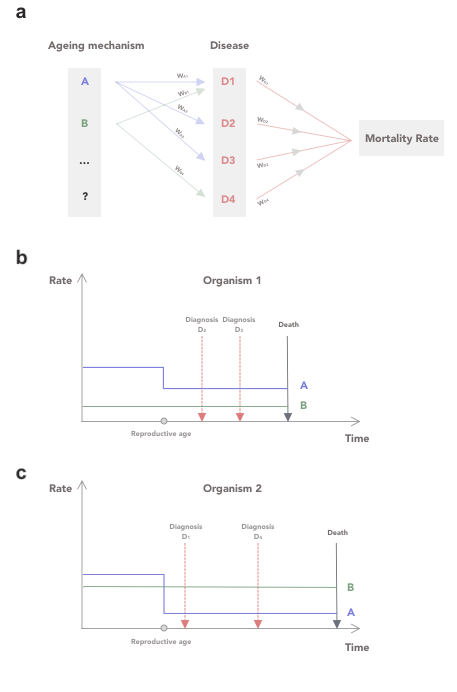
\includegraphics[width=0.8\textwidth]{C1_Fig1}
	\vspace*{1 mm}
	\caption[Theoretical framework to conceptualise the ageing process]{Theoretical framework to conceptualise the ageing process. \textbf{a.} The ageing process is composed of different molecular mechanisms (subprocesses) that are operative at different stages of life and contribute, in variable proportions (specified by the weights), to the appearance of different age-related diseases. Furthermore, the development of different diseases affects the mortality rate and, thus, the probability to die. \textbf{b.} and \textbf{c.} Examples of the life histories of two organisms. In these examples, two ageing mechanisms are operative: A (which changes its rate after reproductive age e.g. activated growth-related pathways) and B (with a constant rate over time e.g. some type of (epi)mutational process). Differences in the mechanisms' profiles lead to differences in the age-related diseases that manifest over the lifespan of the organisms, even though the molecular mechanisms are the same. This, affects the mortality rate and, ultimately, the time-to-death. This figure is inspired by ideas from \cite{Hayflick2007,Gems2015,Peto1997}.}
	\label{fig:c1_fig1}
\end{figure}

\smallskip

\subsection{The genetic basis of ageing}

\smallskip

Given the differences in the lifespan between species and even within species \cite{Jones2013, Gems2000}, it is nowadays clear that the ageing process must have a genetic basis. However, for a long time, the ageing process was thought to be a `haphazard process driven solely by entropy' \cite{Kenyon2005}. Furthermore, in 1935 Clive Maine McCay had shown that caloric restriction (a reduction in calories intake without malnutrition) could extend mean and maximal lifespan in rats \cite{McCay1935,McDonald2010}, which probably shifted the focus towards environmental or external causes as the main driver forces of the ageing process. Since then, dietary restriction (different types of dietary interventions that reduce food intake without malnutrition) has been established as the most successful non-genetic intervention to slow down the ageing process across species \cite{Fontana2015}.

\bigskip

The establishment of the nematode \textit{Caenorhabditis elegans} as a model organism in the 70s triggered its adoption in the ageing field \cite{KLASS1976}, since it allowed well-controlled experiments in a much shorter period of time than rodents \cite{Johnson2013}. This lead to the discovery of the first mutants that dramatically extended lifespan, which mapped to genes in the insulin/IGF-1 signalling pathway \cite{Kenyon1993,Morris1996}. Since then, many genes have been found to significantly affect the lifespan of other model organisms as well, such as budding yeast (\textit{Saccharomyces cerevisiae}), fruit fly (\textit{Drosophila melanogaster}) or mouse (\textit{Mus musculus}) \cite{Kenyon2005,Kenyon2010,Singh2019}. 

\bigskip

Interestingly, the effects of many of these genetic mutations and their pathways are shared by distantly-related species. This suggests that at least part of the molecular mechanisms that drive the ageing process could be evolutionarily conserved. Among these ageing-related signalling pathways it is worth highlighting (Fig.~) \cite{Kenyon2005,Kenyon2010,Singh2019}:

\begin{itemize} 

	\item \textbf{Insulin/IGF-1 pathway}. This underscores the central role of the endocrine system on the biology of ageing. Mutations in \textit{daf-2}, encoding an insulin/IGF-1 receptor, were originally found to double the lifespan of \textit{C. elegans} \cite{Kenyon1993}. Activation of the insulin / IGF-1 pathway, a PI3K pathway, leads to the phosphorylation of a transcription factor of the FOXO family, \textit{daf-16} in \textit{C. elegans}, which prevents it to reach the nucleus \cite{Lin2001}. FOXO transcription factors, of which there are several members in mammals, activate the expression of longevity-promoting genes involved in processes such as autophagy, resistance to oxidative stress or stem cell maintenance \cite{Martins2016}. This partially explains why inhibiting the insulin / IGF-1 pathway can increase organismal lifespan, although other downstream targets, such as \textit{hsf-1} in \textit{C. elegans} (a transcription factor that regulates heat-shock response), also seem to be required \cite{Hsu2003}. 
	
	\item \textbf{\acrshort{TOR} pathway}. Nutrient-sensing. TOR is a protein kinase that phosphorylates ribosomal S6 kinase and translation initiation factor 4E binding protein 1, an inhibitor of the eukaryotic initiation factor 4E, in response to nutrients, which in turn promotes growth (Inoki et al., 2005).
	
	\item \textbf{Sirtuins}. Sir2 --> SirT1 in mammals. NAD dependent. 
	
	\item \textbf{AMPK pathway}.

\end{itemize}

\bigskip

These pathways (especially the insulin/IGF-1 and the TOR pathways) seem to have a dual role depending on the environmental context that the organism is facing. Under abundant nutrient availability and low stress, they tend to promote growth and reproduction. On the contrary, under harsh conditions (such as those posed by dietary restriction), they favour cell protection and maintenance \cite{Kenyon2005,Kenyon2010}. This also relates to the \textbf{disposable soma theory}, where more resources are allocated to reproduction or somatic maintenance depending on the context \cite{Kirkwood1977,Kirkwood1991}. Even though this model is a clear oversimplification, it becomes useful when thinking about the way that the ageing process might have evolved and how the same biological pathways can be repurposed to activate complex genetic programs with completely different goals.

\bigskip

Many more complexities which will require an entire thesis to discuss. Furthermore, the effects of the insulin/IGF-1 pathway seem to be mediated in a cell non-autonomous manner [EXPLAIN], tissue-specific [Tissue-specific activities of the C. elegans DAF-16 protein in the regulation of lifespan, https://www.cell.com/molecular-cell/fulltext/S1097-2765(05)00015-8] and change depending on the "life stage" [Timing requirements for insulin/IGF-1 signaling in C. elegans]. Therefore, the inner workings of the signalling pathways that seem to affect of the ageing process are still a topic of intense research.   



endocrine signaling, stress responses, metabolism, and telomeres
extend life span in response to sensory cues, caloric restriction, or stress
Link between playing with the activation of those pathways and age-related disease, which connects it to the main paradigm we are discussing.
Important take home message: the rate of ageing is plastic and maleable. 
Extreme longevity, playing with several pathways, different increases possible, it gets more difficult with mammals
https://www.ncbi.nlm.nih.gov/pubmed/14576426?dopt=Abstract


AAK-2, AMP kinase; sir-2 --> upstream of daf-16

Summary of pathways: http://jcs.biologists.org/content/121/4/407
Hormesis
Mitochondrial stuff



Hallmarks could be understood of these ageing subprocesses or combinations of them.  


Mammalian ageing. Lifespan, 


Naked mole rat defy ageing. https://elifesciences.org/articles/31157
%Latest review on genetics of ageing https://www.cell.com/cell/fulltext/S0092-8674(19)30221-1?dgcid=raven_jbs_etoc_email

\subsection{Mammalian ageing}

mice have separate receptors for insulin and IGF-1, several FOXOs, upstream regulation by growth hormone (e.g. Ames and Snell dwarf mice; (Brown-Borg et al., 1996
, Flurkey et al., 2002
)).

Response to DR via which pathways.

\subsection{Studying the ageing process in humans}

29th
This suggests that at least part of the molecular mechanisms that drive the ageing process could be conserved and therefore these discoveries translatable to humans
Limits to human lifespan.
Genetics: variation in FOXO 
https://onlinelibrary.wiley.com/doi/full/10.1111/acel.12427
Goal: extending healthspan. What happens in mutants in model organisms:
https://onlinelibrary.wiley.com/doi/full/10.1111/acel.12704
https://www.nature.com/articles/s41586-018-0457-8
Progeroid syndromes.
Centenarians, blue zones.
Differences between males and females.
Exceptional longevity. Centenarians. Blue zones, DNA methylation
https://epigeneticsandchromatin.biomedcentral.com/articles/10.1186/s13072-017-0128-2
Societal consequences
Longitudinal vs cross-sectional, cohorts.
This suggests that at least part of the molecular mechanisms that drive the ageing process could be conserved and therefore these discoveries translatable to humans. Anti-ageing drugs.
Caloric restriction in humans
https://www.ncbi.nlm.nih.gov/pubmed/27544442
In primates: Dietary restriction delays disease onset and mortality in rhesus monkeys


\section{Epigenetics of ageing}

\section{A brief introduction to epigenetics}

30th
Waddington, Chreodes.
Genetics vs environment. How much of the epigenome is genetically programmed.
Epigenetics and development, developmental disorders, imprinting disorders, overgrowth.

Potential energy landscapes identify the information-theoretic nature of the epigenome

Transgenerational epigenetic inheritance of longevity in C. elegans.
https://www.ncbi.nlm.nih.gov/pubmed/22012258


\section{Fundamentals of DNA methylation}

31st
Species / Enzymes / reactions.
Including briefly on technologies, mainly bisulfite sequencing.
As part of the DNA methylation section: Measuring DNA methylation (i.e.table with technologies). Adapt from Advances in the profiling of DNA modifications, Nature Review Genetics
A bit on the mainstream technologies: WGBS, RRBS, arrays (differences between them: e.g. different chemistries), basic principles behind the measurement. Define colour channels, bead, probe, chemistries, …

\section{Epigenetic changes during mammalian ageing}

1st
Remodelling of the mouse epigenome. 
https://www.biorxiv.org/content/10.1101/336172v1

Define hypermethylated / hypermethylation and hypomethylated / hypomethylation.

Age-related epigenetic changes at different levels: histone modifications, m6-RNA https://onlinelibrary.wiley.com/doi/full/10.1111/acel.12753

Put in the context of theory (non-random): %https://www.cell.com/trends/genetics/fulltext/S0168-9525(13)00083-8?_returnURL=https%3A%2F%2Flinkinghub.elsevier.com%2Fretrieve%2Fpii%2FS0168952513000838%3Fshowall%3Dtrue


\section{Epigenetic ageing clocks}

\subsection{Measuring the ageing process}

2nd

At the population level: lifespan curves. 

In all of this it was crucial --> One of the most useful tools used in ageing research are survival curves (aka lifespan curves). PLotting the survival distribution. The mortality rate function can follow different functional forms. Among them, the following form is normally used in ageing experiments \cite{Witten1986}:

\begin{align}
\lambda(t) = h_0 \cdot e^{\gamma t}
\end{align}

where $h_0$ and $\gamma$ are parameters of the model. This leads to the Gompertz survival distribution:

\begin{align}
S(t) = \exp \left[ \frac{h_0}{\gamma} \cdot (1-e^{\gamma t}) \right]
\end{align}


%The mathematical mortality model that fits Drosophila survival data best according to AIC (and BIC criterion) is in most cases the Gompertz %model [35% of all cases (45% for BIC criterion)], closely followed by the Weibull model [29% (35% for BIC criterion)], while for C. elegans, the %Weibull model is fitting best in most cases [51% of all cases (65% for BIC criterion)] and the Gompertz is only the best model in ~ 10% of the %cases. https://onlinelibrary.wiley.com/doi/full/10.1111/acel.12121

In mammals generally Gompertz:
https://www.ncbi.nlm.nih.gov/pubmed/29444805
https://elifesciences.org/articles/31157 

Naked mole rat defy ageing. https://elifesciences.org/articles/31157
%Latest review on genetics of ageing https://www.cell.com/cell/fulltext/S0092-8674(19)30221-1?dgcid=raven_jbs_etoc_email


Big problem at the individual level. Definition of biomarker. Biological age vs chronological age. Other biomarkers, focus on telomere length. 
Conceptual root in the theories based on age changes \cite{Medvedev1990}.

\subsection{The emergence of epigenetic clocks}

3rd

Conceptual root on molecular infidelity framework. At the genomic level, the frequency of this molecular damage (mutations, epimutations) seems to occur with a higher probability in specific regions. 
Holliday's work on DNA methylation, part of theories of biological clock \cite{Medvedev1990}. 
Discuss the tissue-specificity of aDMPs:
https://www.ncbi.nlm.nih.gov/pubmed/29848354
https://www.aging-us.com/article/101666/text

Age-related aDMPs vs mortality DMPs:
https://clinicalepigeneticsjournal.biomedcentral.com/articles/10.1186/s13148-019-0622-4

Bocklandt S, et al.: Epigenetic predictor of age. PLoS One 2011, 6(6):e14821. 10.1371/journal.pone.0014821PubMed Central

Make clarification: when we talk about the ‘epigenetic clock’ we are talking about the changes that the epigenome as a whole (and more specifically, the methylome) undergo upon ageing. If we refer to a specific epigenetic clock model, we will mention the name (e.g. Horvath epigenetic clock, mitotic epigenetic clock, …)

Human (surprinsingly came first)

In this case, biological age estimated by epigenetic clocks (trained on chronological age) is normally referred to epigenetic age. 

Other species. Evolutionary perspective.

Why DNA methylation has been more successful than RNA-seq (more robust across tissues, with the downside that it is more difficult to gain functional insights): https://www.ncbi.nlm.nih.gov/pubmed/23034122

Idea that hypermethylation with age could be more conserved across tissues than hypomethylation with age.
https://genomebiology.biomedcentral.com/articles/10.1186/s13059-016-1064-3

All the time-to-death, mortality rate stuff


\subsection{The landscape of epigenetic clocks}

4th
Statistically speaking, the construction of epigenetic clocks is highly degenerate
https://www.aging-us.com/article/101590/text

Weird tissue cases: germ line?, breast, cerebellum, ...
Rooted on ideas of different ageing rates across tissues:
https://www.ncbi.nlm.nih.gov/pubmed/12397350

Define what I mean by epigenetic ageing clock. Multi-tissue? 


\subsection{What do we know about the epigenetic ageing clock so far?}

5th
Information from the background section in the screening paper.

Association of epigenetic age acceleration with breast cancer risk https://academic.oup.com/jnci/advance-article/doi/10.1093/jnci/djz020/5341521

progeroid syndromes (e.g., Werner syndrome, Hutchinson Gilford Progeria Syndrome; Down syndrome) correlates with accelerated epigenetic aging

The epigenetic clock seems to work in vitro, in cells, explants [] and organoids[]. Also cells from transplant maintain age, so probably cell intrinsic property. Single-cell analysis will figure this out, efforts already made with scRNA-seq clock.


Indeed, the phenomenology of HIV+ patients, after several years of infection, shows striking similarities (regarding T cell subset derangement, T cell clonal expansion and telomere shortening of T cells) with that observed in aged people (Pawelec et al., 1999). It is possible to speculate that prolonged, chronic infections other than HIV, despite being less aggressive, can lead to similar results. Symptoms of accelerated immunosenescence are also present in Down’s syndrome, considered a syndrome of precocious aging (Fabris et al., 1984). [https://www.sciencedirect.com/science/article/pii/S0531556599000686?via%3Dihub#BIB40]. 

Interestingly, epigenetic ageing according to Horvath's epigenetic clock (but not according to other epigenetic clocks, such as Hannum's clock, the skin-blood clock, $PhenoAge$ or $GrimAge$) seems to start a few weeks post-conception in fetal tissues \cite{Hoshino2019}. This could imply that the molecular processes responsible for mammalian ageing, at least at the epigenetic level, are already operative during pre-natal development. This \textbf{molecular continuum between development and ageing} is further reinforced by the fact that \textit{in vitro} reprogramming of somatic cells into \acrshort{iPSCs} reduces epigenetic age to values close to zero (or even negative) both in humans \cite{Horvath2013} and mice \cite{Petkovich2017,Meer2018}, which opens the door to potential rejuvenation therapies \cite{Rando2012,Olova2019}. 

https://www.ncbi.nlm.nih.gov/pmc/articles/PMC3509060/
https://www.ncbi.nlm.nih.gov/pmc/articles/PMC3905065/
https://www.ncbi.nlm.nih.gov/pmc/articles/PMC2956763/
https://www.ncbi.nlm.nih.gov/pubmed/21184773

Reprogramming of epigenetic age
https://www.biorxiv.org/content/10.1101/573386v1


Turning back time with emerging rejuvenation strategies

Caloric restriction and DNA methylation https://genomebiology.biomedcentral.com/articles/10.1186/s13059-017-1187-1


Forced expression of the telomere-extending enzyme telomerase can prevent human cells in culture from undergoing senescence (Bodnar et al., 1998
).overexpressing a protein that lengthens telomeres extends the life span of C. elegans (Joeng et al., 2004
). This is intriguing because the somatic cells of C. elegans are postmitotic, so they are not susceptible to replicative telomere shortening

t is, however, possible that the relatively sudden loss of a substantial proportion of cell replicative potential may account for the physical emaciation and loss of homoeostasis associated with senile decay. Kirkwood evolution of ageing


%!TEX root = ../thesis.tex
%*******************************************************************************
%*********************************** Second Chapter *****************************
%*******************************************************************************

\chapter{Statistical aspects of the epigenetic clock}  

\ifpdf
\graphicspath{{Chapter2/Figs/pdf/}}
\else
\graphicspath{{Chapter2/Figs/svg/}}
\fi


\section{Analysing the blood methylome to study human ageing}

\smallskip

\subsection{Building a DNA methylation dataset from public data}

\smallskip

During the last years large amounts of DNA methylation data have been generated to study complex diseases and ageing \cite{Rakyan2011,Flanagan2015}. Many of these datasets can be obtained from public repositories, such as the NCBI-hosted Gene Expression Omnibus (\acrshort{GEO}) \cite{Edgar2002}. Given its clinical accessibility and ease of collection, blood is one of the most commonly profiled tissues in human DNA methylation studies \cite{Flanagan2015}, including published studies on developmental disorders \cite{Aref-Eshghi2018} (see Chapter 3). Therefore, I decided to use blood as my surrogate tissue to broaden our understanding of the human epigenetic ageing clock.

\bigskip

Furthermore, most of these human datasets have been generated using different versions of the Illumina Infinium array technology, with the Illumina Infinium HumanMethylation450 array (450K) being the most frequently used platform \cite{Flanagan2015}. Additionally, given that the different array versions have different chemistries and biases \cite{Bibikova2009,Bibikova2011,Pidsley2016}, I decided to focus on 450K data for my analyses. Using the \textit{GEOquery} R package \cite{Davis2007}, I programmatically downloaded from GEO all the DNA methylation data that I could find or human blood that satisfied the following criteria:

\begin{itemize}
	
	\item Raw DNA methylation data was available (i.e. IDAT files). This was required so the pre-processing pipeline and the batch effect correction (which requires access to control probes intensities, see `xxxxxxx' section) could be consistently applied across all the samples in the study.
	
	\item Metadata for the samples was available, with the chronological age as an absolute requirement. 
	
	\item In order to study physiological ageing, the blood samples corresponded to humans without any major disease. However, it is important to mention that I could never be completely certain of this, since there could be a lack of diagnosis and/or lack of reporting of the disease in the metadata. 
	
\end{itemize}

\smallskip

This allowed me to assembly a human blood DNA methylation dataset for healthy individuals (after \acrshort{QC}, total $N=2218$) with the characteristics shown in Table~\ref{table:c2_table1}, which spans the entire human lifespan (0.5 to 101 years). Fig.~\ref{fig:c2_fig1} shows that the chronological age distribution is bimodal, with peaks around 10.69 and 58.81 years respectively. This reflects a sampling bias in human population studies, with more data being generated for the periods of postnatal development and during the appearance of age-related disease. However, in order to understand the development of complex diseases as a consequence of the ageing process, efforts should be made to sample people also in their middle ages, before the diseases are normally diagnosed.   


\begin{table}
%\centering
\small
	\begin{tabular}{ p{2cm} p{1cm} p{1cm} p{1cm} p{2cm} p{6cm} }
		\toprule
		\textbf{Batch name} & \textbf{N$_{\female}$} & \textbf{N$_{\male}$} & \textbf{N} & \textbf{Median age (years)} & \textbf{Other comments} \\
		\midrule
		Europe & 0 & 121 & 121 & 10.96 & - \\
		Feb\_2016 & 0 & 1 & 1 & 0.50 & - \\
		GSE104812 & 19 & 29 & 48 & 9.00 & - \\
		GSE111629 & 111 & 124 & 235 &  71.00 & - \\
		GSE40279 & 336 & 314 & 650 & 65.00 & - \\
		GSE41273 & 0 & 51 & 51 & 10.25 & - \\
		GSE42861 & 239 & 96 & 335 & 55.00 & - \\
		GSE51032 & 253 & 78 & 331 & 54.57 & Only people that remained cancer-free in the follow-up after sample collection were included  \\
		GSE55491 & 1 & 5 & 6 & 29.50 & - \\
		GSE59065 & 49 & 46 & 95 & 34.00 & - \\
		GSE61496 & 72 & 78 & 150 & 57.00 & Only one member of each twins pair was included \\
		GSE74432 & 29 & 22 & 51 & 12.00 & - \\
		GSE81961 & 25 & 0 & 25 & 30.05 & - \\
		GSE97362 & 39 & 80 & 119 & 13.00 & - \\
		\midrule
		\textbf{Total} & 1173 & 1045 & 2218 & 55.00 & - \\ 
		\bottomrule
	\end{tabular}
	\vspace*{3mm}
	\caption[Overview of the blood DNA methylation dataset from healthy individuals]{Overview of the blood DNA methylation dataset from healthy individuals. All the batches were downloaded from GEO \cite{Edgar2002}, with the exception of `Europe' and `Feb\_2016', which were generated in-house by our collaborators in Canada (see Chapter 3). $N_{\female}$: number of samples from females. $N_{\male}$: number of samples from males. $N$: total number of samples. These numbers correspond to the samples left after applying quality control (QC, see `Overview of the DNA methylation pre-processing pipeline')}
	\label{table:c2_table1}
\end{table} 


\begin{figure}[htbp!] 
	\centering    
	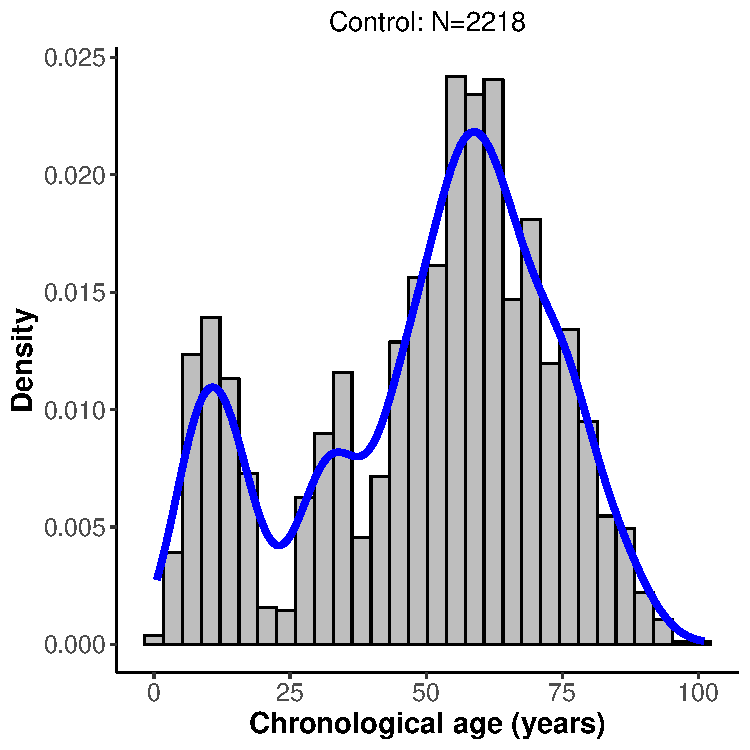
\includegraphics[width=0.6\textwidth]{C2_Fig1}
	\vspace*{2mm}
	\caption[Chronological age distribution in our healthy individuals]{Chronological age distribution in our healthy individuals. Histogram showing the chronological age distribution for all the healthy individuals included in our DNA methylation dataset. The blue line represents the 1D kernel density estimate, as calculate by the \textit{stat\_density} function in R with default parameters.}
	\label{fig:c2_fig1}
\end{figure}

\smallskip

\subsection{Main DNA methylation data pre-processing pipeline}

\smallskip

The analysis of DNA methylation data generated in Illumina arrays has been a topic of huge discussion and statistical innovation in the epigenetic community. There are plenty of reviews in the literature that discuss the different steps that should be involved in the pre-processing of this data type \cite{Wilhelm-Benartzi2013,Morris2015,Liu2016}. More specifically, a recent study by Je Liu and Kimberly D. Siegmund systematically benchmarked the pre-processing methods available for the 450K array in order to reduce variation among technical replicates and improve the detection of biological differences \cite{Liu2016}. Inspired by their results, I implemented, using the \textit{minfi} R package \cite{Aryee2014}, a pre-processing pipeline for the 450K data with the following steps (Fig.~\ref{fig:c2_fig2}):

\begin{enumerate}
	
	
	\item \textbf{Background correction}. I used the \textit{noob} method \cite{TricheJr2013}, as implemented in the \textit{preprocessNoob} function from the \textit{minfi} R package \cite{Aryee2014}. \textit{noob} allows accounting for technical variation in the background (i.e. non-specific) fluorescence signal, which can lead to a reduced dynamic range for the $\beta$-values obtained (Fig.~\ref{fig:c2_fig2}b, Fig.~\ref{fig:sc2_fig1}) \cite{TricheJr2013}. Briefly, when measuring fluorescence intensities in the Illumina array platforms, the observed intensity (also known as foreground, $X_f$) is composed of:
	
	\begin{align}
	X_f = X_s + X_b
	\end{align}
	
	where $X_s$ is the true signal and $X_b$ is the background signal. Making use of a normal-exponential convolution (which assumes $X_b\sim N(\mu, \sigma^2)$ and $X_s\sim Exp(\gamma)$) and the `out-of-band' (\acrshort{OOB}) intensities (fluorescence signals in the opposite colour channel in Infinium I probes) to model $X_b$ , \textit{noob} is capable of estimating $X_s$ given $X_f$. Furthermore, I also applied the default dye-bias correction strategy, which controls for the different average intensities in the two colour channels \cite{TricheJr2013}. 
	
		\item \textbf{Quality control} (QC). Following guidelines from the \textit{minfi} R package \cite{Aryee2014}, I kept only those samples that satisfied the following criteria:
		
		\begin{enumerate}
			
			\item The sex predicted from the DNA methylation data (\acrshort{Sexp}) was the same as the reported sex in the metadata. The sex was predicted  using the \textit{getSex} function from the \textit{minfi} R package \cite{Aryee2014}, which employs intensity information from the sex chromosomes, such that:
			
			\begin{align}
			\text{Sex}_{p} = 
			\begin{cases}
			\text{female, } &\text{if: } (\mathrm{median}\left\{\log_2(M_{y}+U_{y})\right\} -  \mathrm{median}\left\{\log_2(M_{x}+U_{x})\right\}) < c \\
			\text{male, } &\text{if: } (\mathrm{median}\left\{\log_2(M_{y}+U_{y})\right\} -  \mathrm{median}\left\{\log_2(M_{x}+U_{x})\right\}) \geq c \\
			\end{cases}
			\end{align}
			
			where $M_{y}$ and $U_{y}$ represent the methylated and unmethylated intensity measurements for the array probes in the Y chromosome, $M_{x}$ and $U_{x}$ represent the methylated and unmethylated intensity measurements for the array probes in the X chromosome and $c$ is a predefined cutoff (default in \textit{minfi}: $c=-2$).
			
			\smallskip
			
			\item They were not outliers according to their global intensity values after background correction, such that:
			
			\begin{align}
			\frac{\mathrm{median}\left\{\log_2(M_{i})\right\} + \mathrm{median}\left\{\log_2(U_{i})\right\}}{2} \geq 10.5
			\end{align}
			
			where $M_{i}$ and $U_{i}$ represent the background-corrected methylated and unmethylated intensity measurements for all the 450K array probes (Fig.~\ref{fig:sc2_fig2}).
			
		\end{enumerate} 
	
	\item \textbf{Probe filtering}. I filtered out the following types of probes:
	
	\begin{itemize}
		
		\item Probes that contain \acrshort{SNP}s at the single base extension site (position 0) or at the proximal CpG on the probe (positions 1-2), using the \textit{dropLociWithSnps} function in the \textit{minfi} package \cite{Aryee2014}. 
		
		\item Cross-reactive probes, as defined by Chen \textit{et al.} \cite{Chen2013}. These are probes that can co-hybridise to alternative genomic sequences that are highly homologous to the target sequences \cite{Chen2013}.  
		
		\item  Probes that map to the sex chromosomes (X and Y).
	
	\end{itemize}
	
	It is important to mention that other authors have also filtered out probes with high detection p-value or low bead counts across samples \cite{Wilhelm-Benartzi2013,Morris2015}. However, I did not include these filters since it was not pointed out in the \textit{minfi} guidelines \cite{Aryee2014,Fortin2015} and it could complicate further downstream analyses (e.g. different sets of probes missing across different batches, discarding probes that were needed for cell composition estimation, ...).     
	
	
	\begin{figure}[htbp!] 
		\centering    
		\includegraphics[width=0.8\textwidth]{C2_Fig2}
		\vspace*{2mm}
		\caption[Main DNA methylation data pre-processing pipeline]{Main DNA methylation data pre-processing pipeline. \textbf{a.} Flowchart showing the main steps that I implemented to pre-process the DNA methylation data for the healthy individuals. The number of samples (N$_{samples}$) and the number of array probes (N$_{probes}$) left after each step are also specified. \textbf{b.}  $\beta$-value distributions, calculated using the raw fluorescence intensities (i.e. before any pre-processing), for the samples in the GSE41273 batch. Each curve represents a different sample. In grey: 51 samples that passed quality control (QC). In red: 2 samples that failed QC.  \textbf{c.} As in b., but calculating the $\beta$-values after background correction. \textbf{d.} As in b., but calculating the $\beta$-values after background correction, QC, probe filtering and BMIQ normalisation (i.e. the final $\beta$-values that I used for downstream analyses). Note that the samples that failed QC have been removed.}
		\label{fig:c2_fig2}
	\end{figure}
	
	
	\item \textbf{$\beta$-value calculation}. The methylation status of a given CpG site in one of the array probes is normally quantified using the $\beta$-value statistic ($\beta$), which can be calculated as \cite{Wilhelm-Benartzi2013,Du2010}:
	
	\begin{align}
	\beta_i = \frac{\text{max}(M_i,0)}{\text{max}(M_i,0) + \text{max}(U_i,0) + \alpha}
	\end{align}
	
	where $M_i$ and $U_i$ represent the methylated and unmethylated intensity measurements for the $i$th-probe and $\alpha$ is a constant offset (in this work $\alpha = 100$, as recommended by Illumina) \cite{Du2010}. 
	
	In a DNA copy (allele) of a single cell, a specific CpG site is either unmethylated or methylated (categorical / binary variable). However, given that a bulk DNA sample from a tissue is composed of thousands of cells (which can include different cell types with different methylation patterns), $\beta$-values result in a continuous variable between 0 and 1. A value of 0 means that all the measured DNA molecules are unmethylated ($0\%$) and a value of 1 means that all the measured DNA molecules are methylated ($100\%$), which is roughly equivalent to say that 100\% of the cells are either unmethylated or methylated respectively in that CpG site for the sampled tissue. The $\beta$-values for a given sample normally follow a bimodal distribution, where the two peaks are centred around 0 and 1 (Fig.~\ref{fig:c2_fig2}d). 
	
	Other authors have used M-values to quantify methylation levels in arrays (Fig.~\ref{fig:sc2_fig3}), which can be calculated as:
	
	\begin{align}
	\text{M-value}_i = \log_2 \left(\frac{\text{max}(M_i,0) + \alpha}{\text{max}(U_i,0) + \alpha}\right)
	\end{align}
	
	with a default offset value of $\alpha=1$.  Du \textit{et al.} reported that $\beta$-values suffer from severe heteroscedasticity for highly methylated or unmethylated CpG sites and therefore the M-values have more desirable statistical properties \cite{Du2010}. However, Zhuang \textit{et al.} later showed that this only becomes a problem in studies with small sample sizes \cite{Zhuang2012} (which is not the case for my analyses). Furthermore, $\beta$-values are easier to interpret biologically and can be readily used in the context of BMIQ normalisation (see below). For these reasons, I choose $\beta$-values as the main methylation variable for this work.
	
	\item \textbf{Beta-mixture quantile normalisation} (\acrshort{BMIQ}). As mentioned in Chapter 1, in the case of the 450K arrays two types of probes / chemistry coexist in the same platform. Infinium I probes and Infinium II probes have different $\beta$-values distributions (a.k.a. Infinium II probe bias). BMIQ is an intra-array normalisation strategy that allows to correct for this bias and has been shown to outperform other methods used in this context \cite{Teschendorff2012,Dedeurwaerder2011,Touleimat2012,Maksimovic2012}. BMIQ fits a three-state beta-mixture model to Infinium I and Infinium II probes separately and then maps the Infinium II probes distribution into the Infinium I probe distribution (Fig.~\ref{fig:c2_fig3}). In the case of unmethylated ($\beta$-values close to 0) and methylated ($\beta$-values close to 1) probes, this is done by transforming probabilities into quantiles. In the case of `hemimethylated' probes (intermediate $\beta$-values), a dilation transformation is applied to preserve the monotonicity and continuity of the data \cite{Teschendorff2012}. I applied BMIQ to my samples and discarded those that failed the normalisation step.  
	
\end{enumerate}

\bigskip
 
\begin{figure}[htbp!] 
	\centering    
	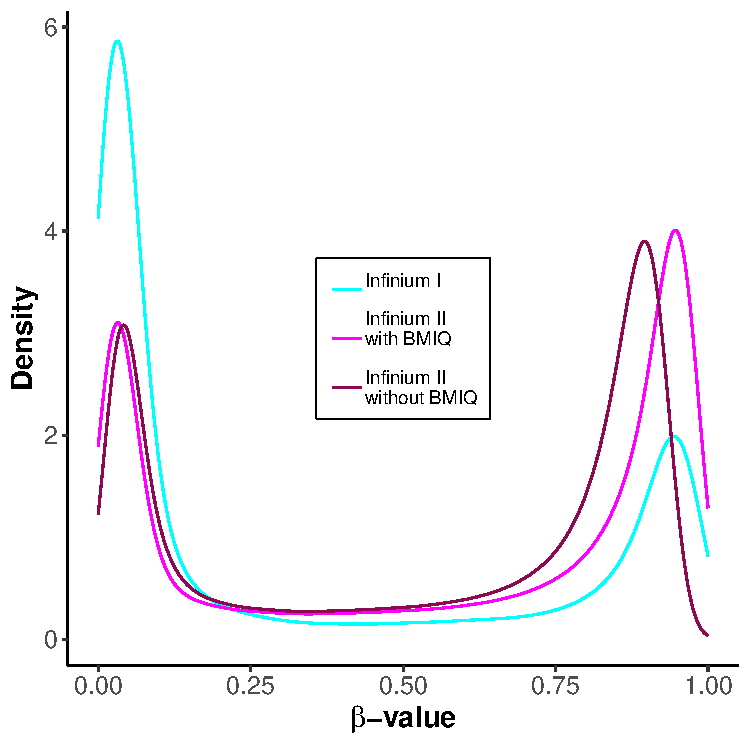
\includegraphics[width=0.8\textwidth]{C2_Fig3}
	\caption[Effect of BMIQ normalisation on the $\beta$-value distribution]{Effect of BMIQ normalisation on the $\beta$-value distribution. The $\beta$-value distributions for different subsets of array probes in a DNA methylation sample from the GSE41273 batch. It can be appreciated how BMIQ transforms the distribution of the Infinium II probes into a distribution more similar to the Infinium I probes.}
	\label{fig:c2_fig3}
\end{figure}

 





\smallskip

\section{Behaviour of Horvath's epigenetic clock during ageing}

\smallskip


\smallskip

\section{Behaviour of other epigenetic clocks during ageing}

\smallskip



\section{Additional methods}

\subsection*{Experimental procedures for DNA methylation data generation}



%!TEX root = ../thesis.tex
%*******************************************************************************
%*********************************** Third Chapter *****************************
%*******************************************************************************

\chapter{Biological aspects}  \label{c:3}

\ifpdf
    \graphicspath{{Chapter3/Figs/Raster/}{Chapter3/Figs/PDF/}{Chapter3/Figs/}}
\else
    \graphicspath{{Chapter3/Figs/Vector/}{Chapter3/Figs/}}
\fi


%********************************** %First Section  **************************************

\epigraph{`At a fundamental level evolutionary survival is the preservation of a dynamic balance between information, or order, and entropy, or disorder.'}{T. B. L. \citet{Kirkwood1977}}


\subsection*{Declaration} 

\footnotesize

This chapter in mainly the product of my own work. Additionally, I would like to recognise the contributions of Janet M. Thornton, Wolf Reik and Thomas M. Stubbs (who helped designing the study and interpreting the data), Erfan Aref-Eshghi (who run some of the analyses using my code and provided part of the samples in the dataset), Marc Jan Bonder and Oliver Stegle (who provided statistical input) and Bekim Sadikovic (who provided part of the samples in the dataset). All of them also helped in the revision of the final text. This work has been published in the journal \textit{Genome Biology} \citep{Martin-Herranz2019a}.

\normalsize

\section{Background} 

\smallskip

Epigenetic clocks can be understood as a proxy to quantify the changes of the epigenome with age. However, little is known about the molecular mechanisms that determine the rate of the underlying epigenetic ageing clock (see section~\ref{s:1.3.3}). Steve Horvath proposed that the multi-tissue epigenetic clock captures the workings of an \textbf{epigenetic maintenance system} \citep{Horvath2013}. Recent \acrshort{GWAS} studies have found several genetic variants associated with epigenetic age acceleration in genes such as \textit{TERT} (the catalytic subunit of telomerase) \citep{Lu2018}, \textit{DHX57} (an ATP-dependent RNA helicase) \citep{Lu2016} or \textit{MLST8} (a subunit of both mTORC1 and mTORC2 complexes) \citep{Lu2016}. Nevertheless, to my knowledge no genetic variants in epigenetic modifiers have been found and the molecular nature of this hypothetical system is unknown to this date.

\bigskip

I decided to take a reverse genetics approach and look at the \textbf{behaviour of the epigenetic clock in patients with developmental disorders}, many of which harbour mutations in proteins of the epigenetic machinery \citep{Aref-Eshghi2018,Bjornsson2015}. I performed an unbiased screen for epigenetic age acceleration and found that Sotos syndrome accelerates epigenetic ageing, potentially revealing a role of H3K36 methylation maintenance in the regulation of the rate of the epigenetic clock.

\smallskip

\section{Screening for genes that accelerate the epigenetic \\ageing clock} \label{s:3.2}

\smallskip

The main goal of this analysis is to identify genes, mainly components of the epigenetic machinery, that can \textbf{affect the rate of epigenetic ageing in humans} (as measured by Horvath’s epigenetic clock) \citep{Horvath2013}. For this purpose, I assembled a dataset with all the DNA methylation data from patients with different developmental disorders that I could find, in order to perform an unbiased screen. This dataset combines samples publicly available in GEO \citep{Edgar2002} with in-house data generated by my collaborators at the London Health Sciences Centre, Canada (Table~\ref{table:s2_table1}, Fig.~\ref{fig:sc3_fig1}). All these data were generated from blood using the Illumina 450K methylation array, as in the case of the healthy individuals described in Chapter~\ref{c:2}.   

\bigskip

Many of these developmental syndromes have overlapping clinical features \citep{Aref-Eshghi2018, Bjornsson2015}. Furthermore, in some cases with a clinical diagnosis, the genetic cause remains unknown, probably due to locus heterogeneity or difficulty to assess the clinical significance of some genetic variants \citep{Aref-Eshghi2017}. Therefore, several studies have explored the ability of DNA methylation signatures to aid differential diagnoses of these syndromes \citep{Aref-Eshghi2018,Aref-Eshghi2017,Aref-Eshghi2018a,Butcher2017,Choufani2015,Schenkel2016,Alisch2013,Schenkel2017,Hood2016,Aldinger2013,Grafodatskaya2013,Kernohan2016}. Given that most of the diagnoses for developmental disorders are carried out early in life, this dataset has a bias towards younger ages (Fig.~\ref{fig:c3_fig1}). In order to maximise the ability to detect ageing-associated effects, I kept only those developmental disorders with at least 5 samples, of which at least 2 had a chronological age $\geq 20$ years (which, according to Horvath's model, is the adult age for humans) \citep{Horvath2013}. This filtering resulted in a dataset for the main screen with $N = 367$ samples from cases, which had ages between 0 and 55 years (Fig.~\ref{fig:c3_fig2}, Table~\ref{table:c3_table1}).

\begin{figure}[htbp!] 
	\centering
	\vspace*{6mm}    
	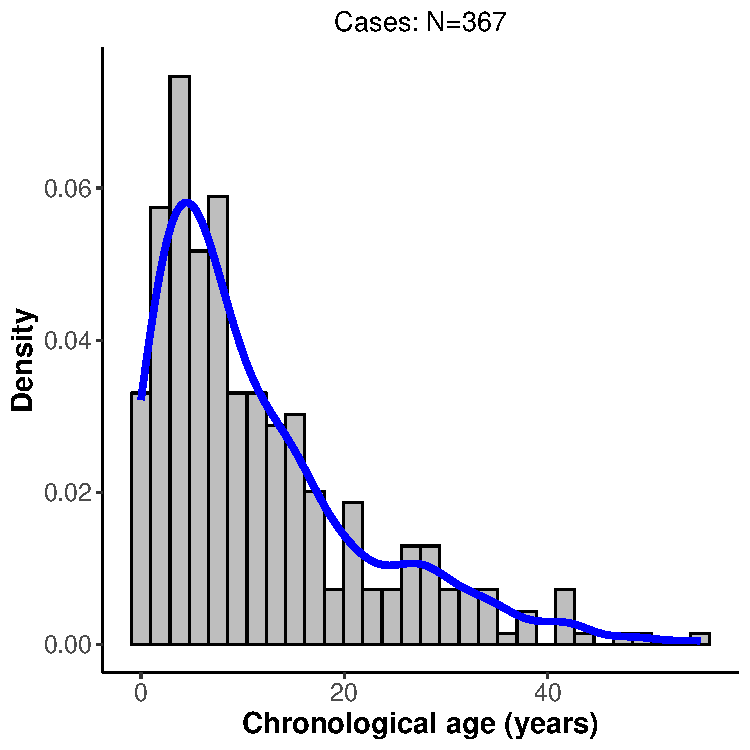
\includegraphics[width=0.6\textwidth]{C3_Fig1}
	\vspace*{2mm}
	\caption[Chronological age distribution in the individuals with developmental disorders]{Histogram showing the chronological age distribution for all the individuals with developmental disorders (cases) included in the final dataset (i.e. after QC and filtering). The blue line represents the 1D kernel density estimate, as calculate by the \textit{stat\_density} function in R with default parameters.}
	\label{fig:c3_fig1}
\end{figure}

\begin{figure}[htbp!] 
	\centering    
	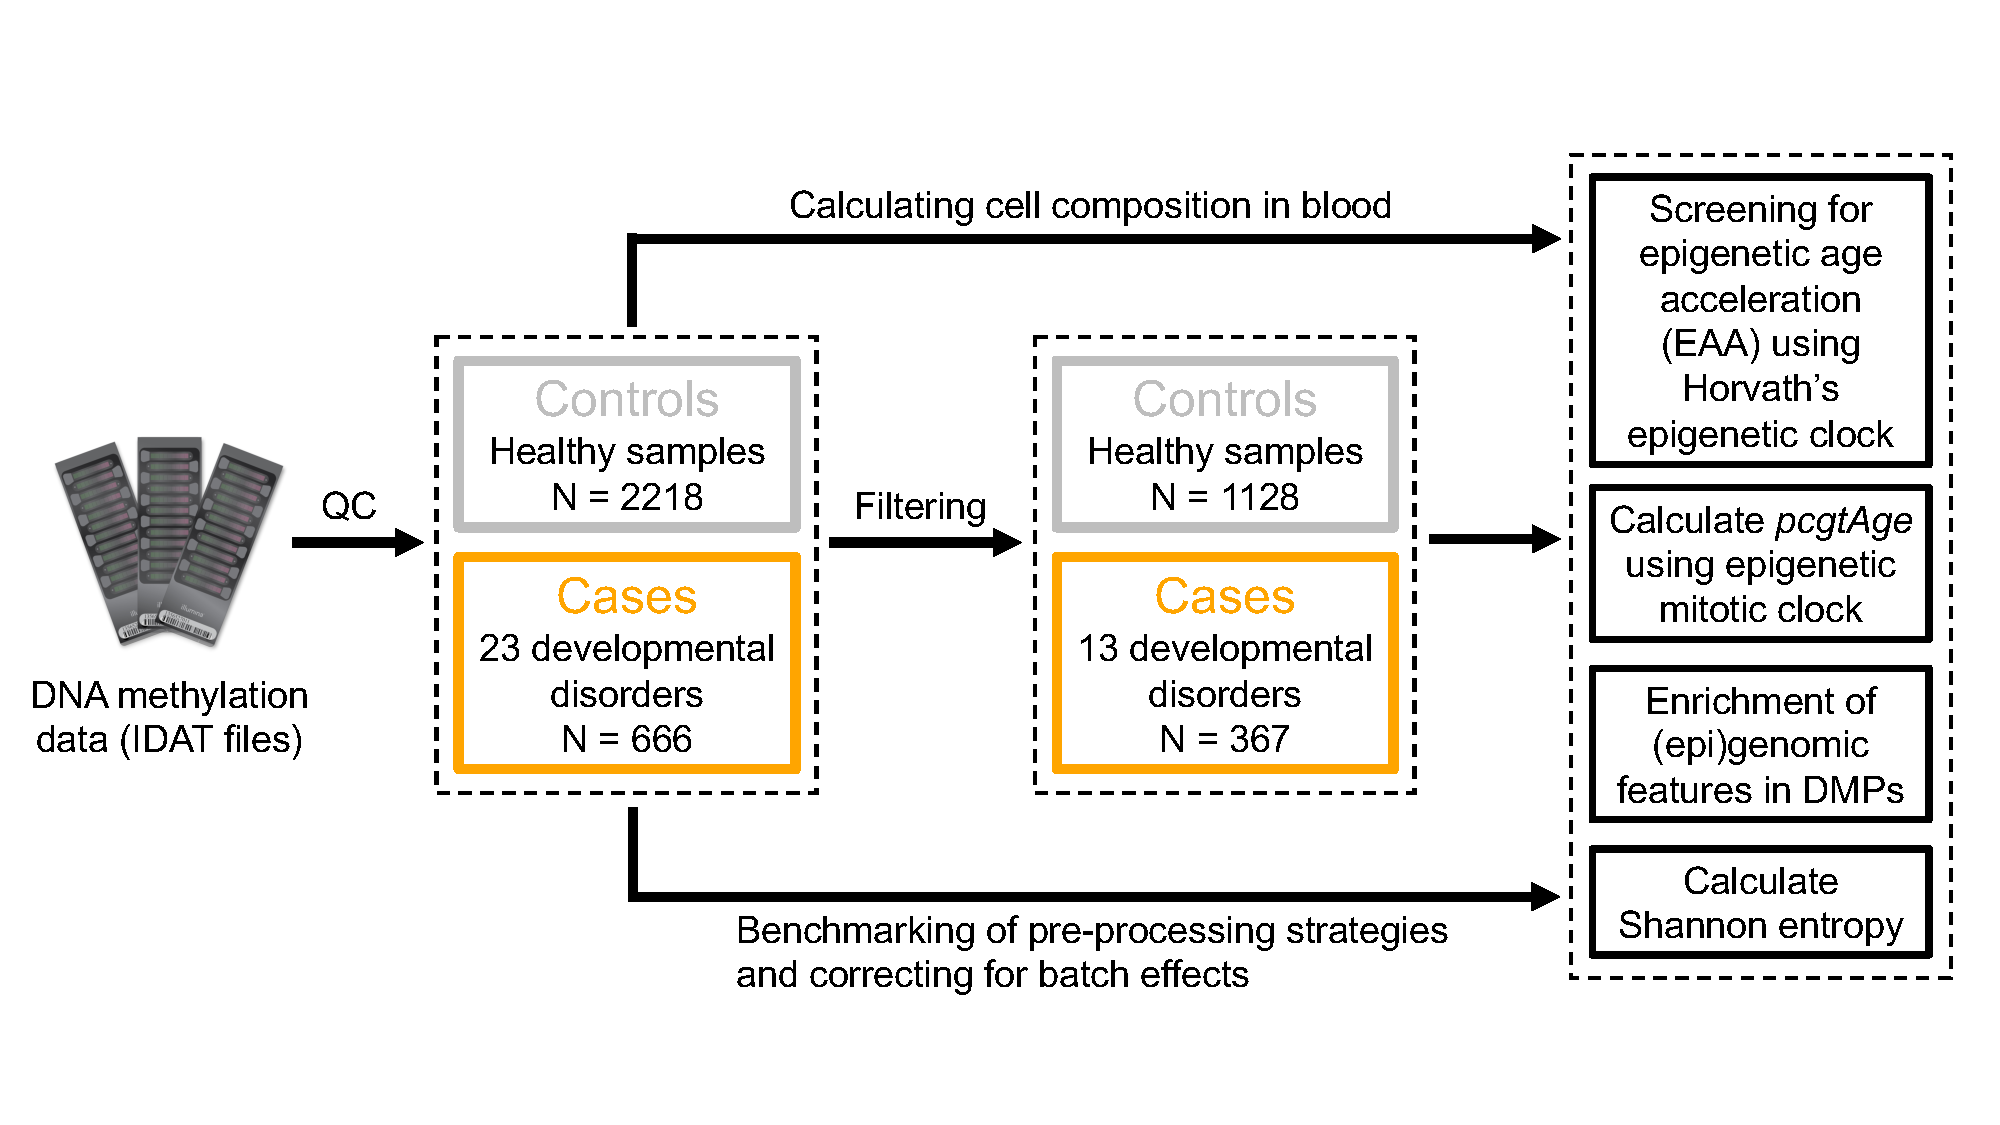
\includegraphics[width=1\textwidth]{C3_Fig2}
	\caption[Overview of the analyses performed in Chapter~\ref{c:3}]{Flow diagram that portrays an overview of the different analyses that are carried out in the raw DNA methylation data (IDAT files) from human blood for cases (developmental disorders samples) and controls (healthy samples). The control samples are filtered to match the age range of the cases (0-55 years). The cases are filtered based on the number of `adult’ samples available (for each disorder, at least 5 samples, with 2 of them with an age $\geq$ 20 years). QC: quality control. DMPs: differentially methylated positions.}
	\label{fig:c3_fig2}
\end{figure}

\begin{table}
	%\centering
	\small
	\begin{tabular}{ p{4cm} p{2cm} p{2cm} p{2cm} p{1cm} p{2cm} }
		\toprule
		\textbf{Developmental disorder} & \textbf{Gene(s) involved} & \textbf{Gene(s) function} & \textbf{Molecular cause} & \textbf{N} & \textbf{Age range (years)} \\
		\midrule
		Angelman & \textit{UBE3A} & Ubiquitin protein ligase E3A & Imprinting, mutation & 14 & 1 to 55 \\
		\midrule
		Autism spectrum disorder (ASD) & - & - & - & 119 & 1.83 to 35.16 \\
		\midrule
		Alpha thalassemia/mental retardation X-linked syndrome (ATR-X) & \textit{ATRX} &Chromatin remodelling & Mutation & 15 & 0.7 to 27 \\
		\midrule
		Claes-Jensen & \textit{KDM5C} & H3K4 demethylase & Mutation & 10 & 2 to 42 \\
		\midrule
		Coffin-Lowry & \textit{RPS6KA3} & Serine / threonine kinase & Mutation & 10 & 1.3 to 22.8 \\
		\midrule
		Floating-Harbour & \textit{SRCAP} & Chromatin remodelling & Mutation & 17 & 4 to 42 \\
		\midrule
		Fragile X syndrome (FXS) & \textit{FMR1} & Translational control & Mutation (CGG expansion) & 32 & 0.08 to 48 \\
		\midrule
		Kabuki & \textit{KMT2D} & H3K4 methyltransferase & Mutation & 46 & 0 to 24.1 \\
		\midrule
		Noonan & \textit{PTPN11}, \textit{RAF1}, \textit{SOS1} & RAS/ MAPK signalling & Mutation & 15, 11, 14 & 0.2 to 49 \\
		\midrule
		Rett & \textit{MECP2} & Transcriptional repression & Mutation & 15 & 1 to 34 \\
		\midrule
		Saethre-Chotzen & \textit{TWIST1} & Transcription factor & Mutation & 22 & 0 to 38 \\
		\midrule
		Sotos & \textit{NSD1} & H3K36 methyltransferase & Mutation & 20 & 1.6 to 41 \\
		\midrule
		Weaver & \textit{EZH2} & H3K27 methyltransferase & Mutation & 7 & 2.58 to 43 \\
		\midrule
		\textbf{Total} & - & - & - & 367 & 0 to 55  \\ 
		\bottomrule
	\end{tabular}
	\vspace*{3mm}
	\caption[Overview of the developmental disorders that were included in the screening]{Overview of the developmental disorders that were included in the screening after quality control and filtering (total $N=367$).}
	\label{table:c3_table1}
\end{table} 

\bigskip

The purpose of the screen is to \textbf{test whether the epigenetic ages of the samples from a given developmental disorder (cases) deviate from their chronological age} i.e. identify those developmental disorders that present epigenetic age acceleration (EAA). For a given sample, a positive EAA indicates that the epigenetic (biological) age of the sample is higher than the one expected for someone with that chronological age. In other words, it means that the epigenome of that person resembles the epigenome of an older individual. The opposite is true when a negative EAA is found (i.e. the epigenome looks younger than expected). I calculated the epigenetic ages ($DNAmAge$) of all the samples according to Horvath's epigenetic clock (see section~\ref{s:2.2.1}) and I fitted the control models to the samples from the healthy individuals, including models with and without blood cell composition correction (CCC) and always accounting for potential batch effects (see equations \ref{eq:2.16} and \ref{eq:2.17}).  As previously discussed (see section~\ref{s:2.2.2}), due to the fact that Horvath's model underestimates the epigenetic age of old samples, the age distribution of the control samples can have an impact on the results of the screen. Therefore, I filtered the ages of the healthy individual samples to make them match the age range of the developmental disorders (0-55 years, $N = 1128$, see Fig.~\ref{fig:c3_fig2}).

\bigskip

The EAA for the control samples corresponds to the residuals from the control models (see section~\ref{s:2.2.2}). On the other hand, the EAA for a case sample is calculated by taking the difference between the epigenetic age ($DNAmAge$) and the predicted value from the corresponding control model (with or without cell composition). Finally, I compared the distributions of the EAA for the different developmental disorders against the EAA distributions for the healthy controls using the non-parametric two-sided Wilcoxon's test. P-values were adjusted for multiple testing using Bonferroni correction and a significance level of $\alpha = 0.01$ was applied. It is worth mentioning that some of the developmental disorders included in the screen (such as autism spectrum disorder or Coffin-Lowry syndrome) are not necessarily caused by alterations in the epigenetic machinery, but were still included to maintain the unbiased nature of the screen. 

\smallskip

\section{Sotos syndrome accelerates epigenetic ageing}

\smallskip

The results from the screen are portrayed in Fig.~\ref{fig:c3_fig3}. Most syndromes do not show evidence of accelerated epigenetic ageing, but \textbf{Sotos syndrome presents a clear positive EAA} (median EAA$_{\text{with CCC}}$ = + 7.64 years, median EAA$_{\text{without CCC}}$ = + 7.16 years), with p-values considerably below the significance level of 0.01 after Bonferroni correction (p-value$_{\text{corrected, with CCC}}$ = 3.40 $\cdot$ 10$^{-9}$, p-value$_{\text{corrected, without CCC}}$ = 2.61 $\cdot$ 10$^{-7}$). Additionally, Rett syndrome (median EAA$_{\text{with CCC}}$ = + 2.68 years, median EAA$_{\text{without CCC}}$ = + 2.46 years, p-value$_{\text{corrected, with CCC}}$ = 0.0069, p-value$_{\text{corrected, without CCC}}$ = 0.0251) and Kabuki syndrome (median EAA$_{\text{with CCC}}$ = - 1.78 years, median EAA$_{\text{without CCC}}$ = - 2.25 years, p-value$_{\text{corrected, with CCC}}$ = 0.0011, p-value$_{\text{corrected, without CCC}}$ = 0.0035) reach significance, with a positive and negative EAA respectively. Finally, fragile X syndrome (FXS) shows a positive EAA trend (median EAA$_{\text{with CCC}}$ = + 2.44 years, median EAA$_{\text{without CCC}}$ = + 2.88 years) that does not reach significance in the screen (p-value$_{\text{corrected, with CCC}}$ = 0.0680, p-value$_{\text{corrected, without CCC}}$ = 0.0693).

\bigskip

\begin{figure}[htbp!] 
	\centering    
	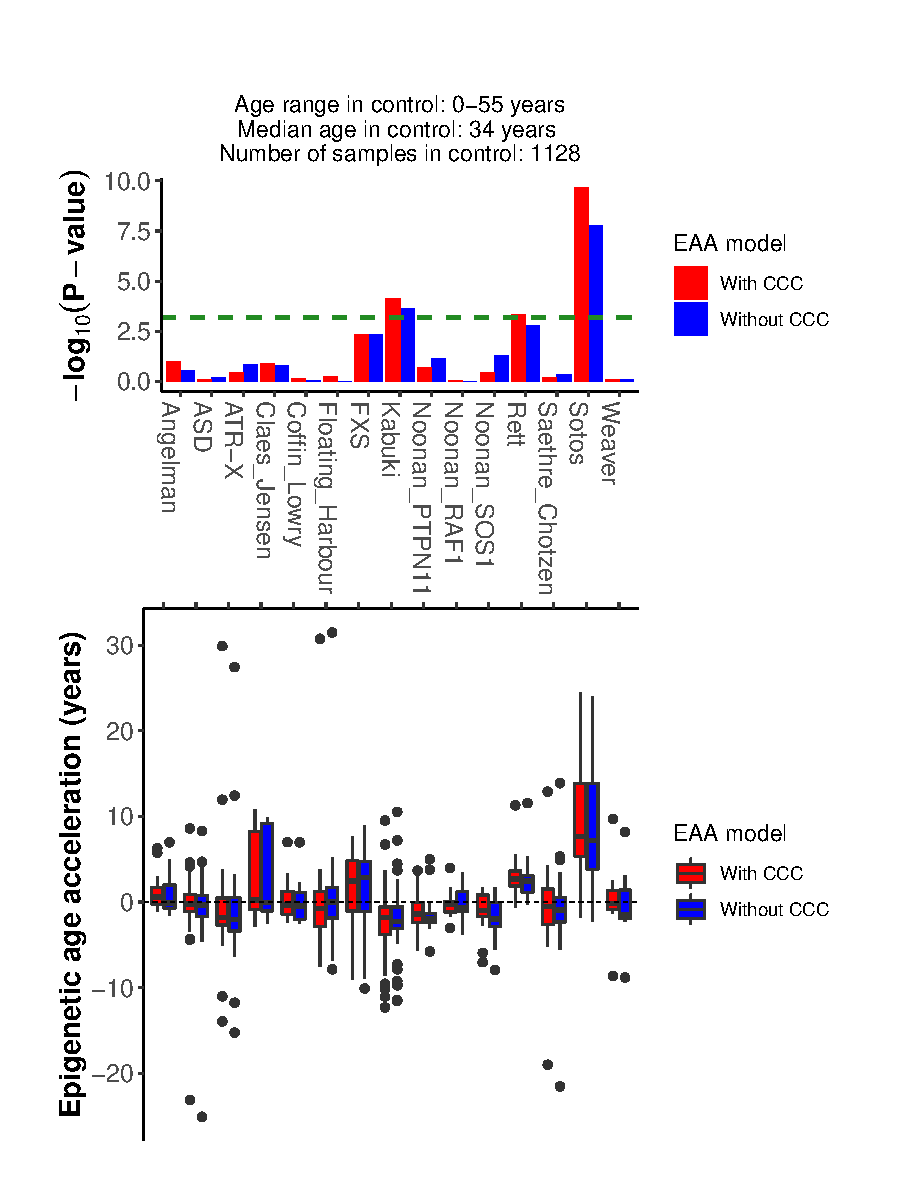
\includegraphics[width=1\textwidth]{C3_Fig3}
	\caption[Screening for epigenetic age acceleration (EAA) in developmental disorders]{Screening for epigenetic age acceleration (EAA) in developmental disorders. The upper panel shows the p-values derived from comparing the EAA distributions for the samples in a given developmental disorder and the control (two-sided Wilcoxon’s test). The dashed green line displays the significance level of $\alpha = 0.01$ after Bonferroni correction. The bars above the green line reach statistical significance. The lower panel displays the actual EAA distributions, which allows assessing the direction of the EAA (positive or negative). In red: EAA model with cell composition correction (CCC). In blue: EAA model without CCC. ASD: autism spectrum disorder. ATR-X: alpha thalassemia/mental retardation X-linked syndrome. FXS: fragile X syndrome.}
	\label{fig:c3_fig3}
\end{figure}

Next, I tested the effect of changing the median age used to build the healthy control model (i.e. the median age of the controls) on the screening results (Fig.~\ref{fig:sc3_fig2}). Sotos syndrome is robust to these changes, whilst Rett, Kabuki and FXS are much more sensitive to the control model used. This again highlights the importance of choosing an appropriate age-matched control when testing for epigenetic age acceleration, given that Horvath’s epigenetic clock underestimates epigenetic age for advanced chronological ages \citep{ElKhoury2018,Marioni2018}.

\bigskip

Moreover, all but one of the Sotos syndrome patients (19/20 = 95\%) show a consistent deviation in EAA (with CCC) in the same direction (Fig.~\ref{fig:c3_fig4}a,b), which is not the case for the rest of the disorders, with the exception of Rett syndrome (Fig.~\ref{fig:sc3_fig3}). Even though these data suggest that there are already some methylomic changes at birth, the EAA seems to increase with age in the case of Sotos patients (Fig.~\ref{fig:c3_fig4}b). This implies that at least some of the changes that normally affect the epigenome with age are happening at a faster rate in Sotos syndrome patients during their lifespan (as opposed to the idea that the Sotos epigenetic changes are only acquired during prenatal development and remain constant afterwards).

\begin{figure}[htbp!] 
	\centering    
	\includegraphics[width=1\textwidth]{C3_Fig4}
	\caption[Sotos syndrome accelerates epigenetic ageing]{Sotos syndrome accelerates epigenetic ageing. \textbf{a.} Scatterplot showing the relationship between epigenetic age ($DNAmAge$) according to Horvath’s model \citep{Horvath2013} and chronological age of the samples for Sotos (orange) and control (grey). Each sample is represented by one point. The black dashed line represents the diagonal to aid visualisation. \textbf{b.} Scatterplot showing the relationship between the epigenetic age acceleration (EAA) and chronological age of the samples for Sotos (orange) and control (grey). Each sample is represented by one point. The yellow line represents the linear model EAA $\sim$ Age, with the standard error shown in the light yellow shade. \textbf{c.} Scatterplot showing the relationship between the score for the epigenetic mitotic clock ($pcgtAge$) \citep{Yang2016} and chronological age of the samples for Sotos (orange) and control (grey). Each sample is represented by one point. A higher value of $pcgtAge$ is associated with a higher number of cell divisions in the tissue. \textbf{d.} Scatterplot showing the relationship between the epigenetic mitotic clock ($pcgtAge$) acceleration (with CCC) and chronological age of the samples for Sotos (orange) and control (grey). Each sample is represented by one point. The yellow line represents the linear model pcgtAge\_EAA$_{\text{with CCC}}$ $\sim$ Age, with the standard error shown in the light yellow shade.}
	\label{fig:c3_fig4}
\end{figure}

\bigskip

Finally, I investigated whether Sotos syndrome leads to a higher rate of (stem) cell division in blood when compared with the healthy population. I employed the epigenetic mitotic clock, that makes use of the fact that some CpGs in promoters that are bound by Polycomb group proteins become hypermethylated with age (captured by a metric called $pcgtAge$; see section~\ref{s:2.3.2}). This hypermethylation correlates with the number of cell divisions in the tissue and is also associated with an increase in cancer risk \citep{Yang2016}. I calculated $pcgtAge$ for the Sotos samples and compared them against the healthy controls (using a model similar to the one in equation \ref{eq:2.16}, although in this case the dependent variable was $pcgtAge$; see section~\ref{s:2.3.2}). I found a trend suggesting that \textbf{the epigenetic mitotic clock might be accelerated in Sotos patients} (p-value = 0.0112, Fig.~\ref{fig:c3_fig4}c,d), which could explain the higher cancer predisposition reported in these patients and might relate to their overgrowth \citep{Leventopoulos2009}.

\bigskip

Consequently, I report that individuals with Sotos syndrome present an accelerated epigenetic age, which makes their epigenome look, on average, more than 7 years older than expected. These changes seem to be the consequence of a higher ticking rate of the epigenetic ageing clock (or at least part of its machinery), with epigenetic age acceleration increasing during lifespan: the youngest Sotos patient (1.6 years) has an EAA$_{\text{with CCC}}$ = 5.43 years and the oldest (41 years) has an EAA$_{\text{with CCC}}$ = 24.53 years. Additionally, Rett syndrome, Kabuki syndrome and fragile X syndrome could also have their epigenetic ages affected, but more evidence is required to be certain about this conclusion.


\section{Comparing Sotos syndrome and physiological ageing}

\smallskip

Sotos syndrome is caused by loss-of-function heterozygous mutations in the NSD1 gene, a histone H3K36 methyltransferase \citep{Choufani2015, Kurotaki2002}. These mutations lead to a specific DNA methylation signature in Sotos patients, potentially due to the crosstalk between the histone and DNA methylation machinery \citep{Choufani2015}. In order to gain a more detailed picture of the reported epigenetic age acceleration, I decided to compare the genome-wide (or at least array-wide) changes observed in the methylome during ageing with those observed in Sotos syndrome. For this purpose, I \textbf{identified differentially methylated positions (DMPs) for both conditions}, using the models that account for cell composition correction (see equations~\ref{eq:2.10} and \ref{eq:3.1}). Ageing DMPs (aDMPs) were calculated in this case using the healthy samples in the age range 0-55 years. aDMPs were composed almost equally of CpG sites that gain methylation with age (i.e. become hypermethylated, 51.69\%) and CpG sites that lose methylation with age (i.e. become hypomethylated, 48.31\%, barplot in Fig.~\ref{fig:c3_fig5}a), a picture that resembles previous studies \citep{Zhu2018}. It is worth mentioning that in this case fewer aDMPs were identified when compared with the full lifespan analysis presented in section~\ref{s:2.1.4}, where the hypomethylated aDMPs were also slightly more frequent when compared with the hypermethylated ones. This highlights the importance of the age range and/or the sample size when calculating aDMPs. On the contrary, DMPs in Sotos were clearly dominated by CpGs that have lower methylation levels in individuals with the syndrome (i.e. hypomethylated, 99.27\%, barplot in Fig.~\ref{fig:c3_fig5}a), consistent with previous reports \citep{Choufani2015}.

\begin{figure}[htbp!] 
	\centering    
	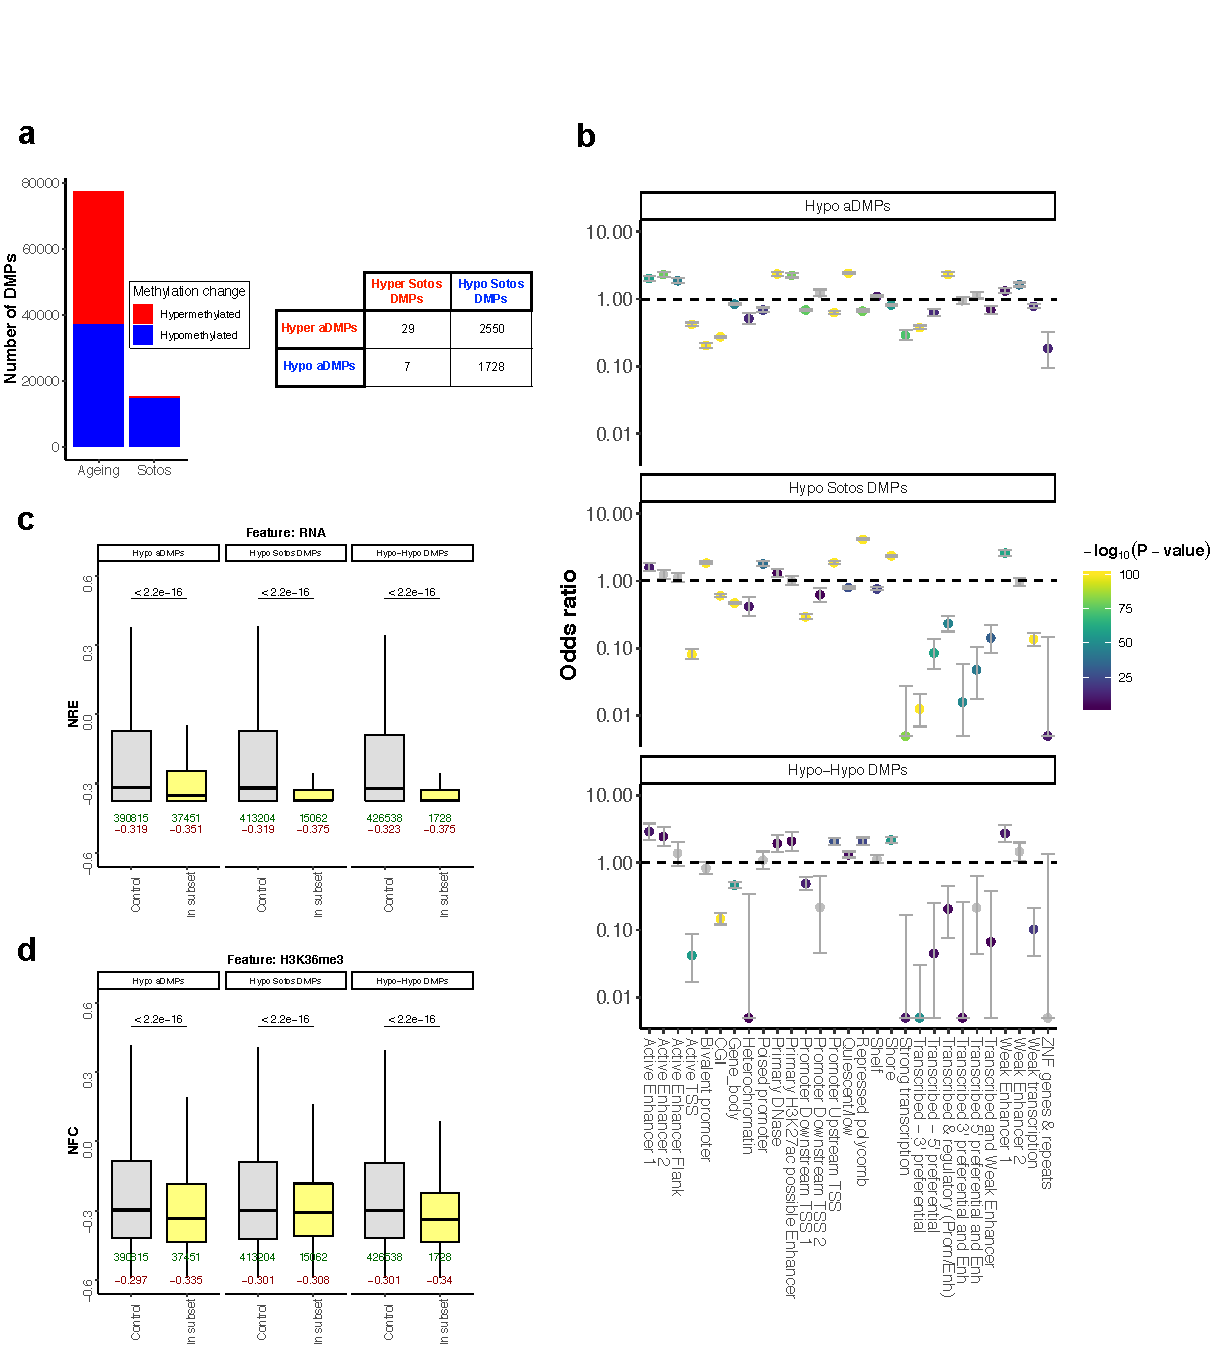
\includegraphics[width=1\textwidth]{C3_Fig5}
	\caption[Comparing DNA methylation changes in Sotos syndrome and physiological ageing]{Comparison between the DNA methylation changes during physiological ageing and in Sotos. \textbf{a.} On the left: barplot showing the total number of differentially methylated positions (DMPs) found during physiological ageing and in Sotos syndrome. CpG sites that increase their methylation levels with age in the healthy population or those that are elevated in Sotos patients (when compared with a control) are displayed in red. Conversely, those CpG sites that decrease their methylation levels are displayed in blue. On the right: table that represents the intersection between the ageing (aDMPs) and the Sotos DMPs. The subset resulting from the intersection between the hypomethylated DMPs in ageing and Sotos is called the `Hypo-Hypo DMPs’ subset (N=1728). \textbf{b.} Enrichment for the categorical (epi)genomic features considered when comparing the different genome-wide subsets of differentially methylated positions (DMPs) in ageing and Sotos against a control (see section~\ref{s:3.7}). The y-axis represents the odds ratio (\acrshort{OR}), the error bars show the 95\% confidence interval for the OR estimate and the colour of the points codes for $-\log_{10}(\text{p-value})$ obtained after testing for enrichment using Fisher's exact test. An OR > 1 shows that the given feature is enriched in the subset of DMPs considered, whilst an OR < 1 shows that it is found less than expected. In grey: features that did not reach significance using a significance level of $\alpha = 0.01$ after Bonferroni correction. \textbf{c.} Boxplots showing the distributions of the `normalised RNA expression' (\acrshort{NRE}) when comparing the different genome-wide subsets of differentially methylated positions (DMPs) in ageing and Sotos against a control (see section~\ref{s:3.7}). NRE represents normalised mean transcript abundance in a window of $\pm$ 200 bp from the CpG site coordinate (DMP) being considered. The p-values (two-sided Wilcoxon's test, before multiple testing correction) are shown above the boxplots. The number of DMPs belonging to each subset (in green) and the median value of the feature score (in dark red) are shown below the boxplots. \textbf{d.} As in c., but showing the `normalised fold change' (\acrshort{NFC}) for the H3K36me3 histone modification (representing normalised mean ChIP-seq fold change for H3K36me3 in a window of $\pm$ 200 bp from the DMP being considered).}
	\label{fig:c3_fig5}
\end{figure}


\bigskip

Then, I compared the intersections between the hypermethylated and hypomethylated DMPs in ageing and Sotos. Most of the DMPs were specific for ageing or Sotos (i.e. they did not overlap), but a subset of them were shared (table in Fig.~\ref{fig:c3_fig5}a). Interestingly, there were 1728 DMPs that became hypomethylated both during ageing and in Sotos (\textbf{`Hypo-Hypo DMPs'}). This subset of DMPs is of special interest because it could be used to understand in more depth some of the mechanisms that drive hypomethylation during physiological ageing. Thus, I tested whether the different subsets of DMPs are found in specific genomic contexts (Fig.~\ref{fig:sc3_fig4}, Fig.~\ref{fig:sc3_fig5}). DMPs that are hypomethylated during ageing and in Sotos were both enriched (odds ratio >1) in enhancer categories (such as `active enhancer 1' or `weak enhancer 1', see the chromatin state model used, from the K562 cell line, in section~\ref{s:3.7}) and depleted (odds ratio <1) for active transcription categories (such as `active TSS' or `strong transcription'), which was also observed in the `Hypo-Hypo DMPs' subset (Fig.~\ref{fig:c3_fig5}b). Interestingly, age-related hypomethylation in enhancers seems to be a characteristic of both humans \citep{Slieker2016,Slieker2018} and mice \citep{Cole2017}. Furthermore, both \textit{de novo} DNA methyltransferases (DNMT3A and DNMT3B) have been shown to bind in an H3K36me3-dependent manner to active enhancers \citep{Rinaldi2016}, consistent with these results.

\bigskip

When looking at the levels of total RNA expression (depleted for \acrshort{rRNA}) in blood, I confirmed a significant reduction in the RNA levels around these hypomethylated DMPs when compared with the controls sets (Fig.~\ref{fig:c3_fig5}c, see section~\ref{s:3.7} for more details on how the control sets were defined). Interestingly, hypomethylated DMPs in both ageing and Sotos were depleted from gene bodies (Fig.~\ref{fig:c3_fig5}b) and were located in areas with lower levels of H3K36me3 when compared with the control sets (Fig.~\ref{fig:c3_fig5}d, Fig.~\ref{fig:sc3_fig5}). Moreover, hypomethylated aDMPs and hypomethylated Sotos DMPs where both generally enriched or depleted for the same histone marks in blood (Fig.~\ref{fig:sc3_fig5}), which adds weight to the hypothesis that they share the same genomic context and could become hypomethylated through similar molecular mechanisms.

\bigskip

Intriguingly, I also identified a subset of DMPs (2550) that were hypermethylated during ageing and hypomethylated in Sotos (Fig.~\ref{fig:c3_fig5}a). These \textbf{`Hyper-Hypo DMPs'} seem to be enriched for categories such as `bivalent promoter' and `repressed polycomb' (Fig.~\ref{fig:sc3_fig4}), which are normally associated with developmental genes \citep{Bernstein2006,Bernhart2016}. These categories are also a defining characteristic of the hypermethylated aDMPs, highlighting that even though the direction of the DNA methylation changes is different in some ageing and Sotos DMPs, the genomic context in which they happen is shared.

\bigskip

Finally, I looked at the DNA methylation patterns in the 353 \textbf{Horvath's epigenetic clock CpG sites for the Sotos samples}. For each clock CpG site, I modelled the changes of DNA methylation with age in the healthy control individuals (0-55 years) and then calculated the deviations from these patterns for the Sotos samples (Fig.~\ref{fig:c3_fig6}, see equation~\ref{eq:3.4}). As expected, the landscape of clock CpG sites is dominated by hypomethylation in the Sotos samples, although only a small fraction of the clock CpG sites seems to be significantly affected (Fig.~\ref{fig:c3_fig6}c). Overall, I confirmed the trends reported for the genome-wide analysis (Fig.~\ref{fig:sc3_fig6}, Fig.~\ref{fig:sc3_fig7}, Fig.~\ref{fig:sc3_fig8}). However, given the much smaller number of CpG sites to consider in this analysis, very few comparisons reached significance.

\begin{figure}[htbp!] 
	\centering    
	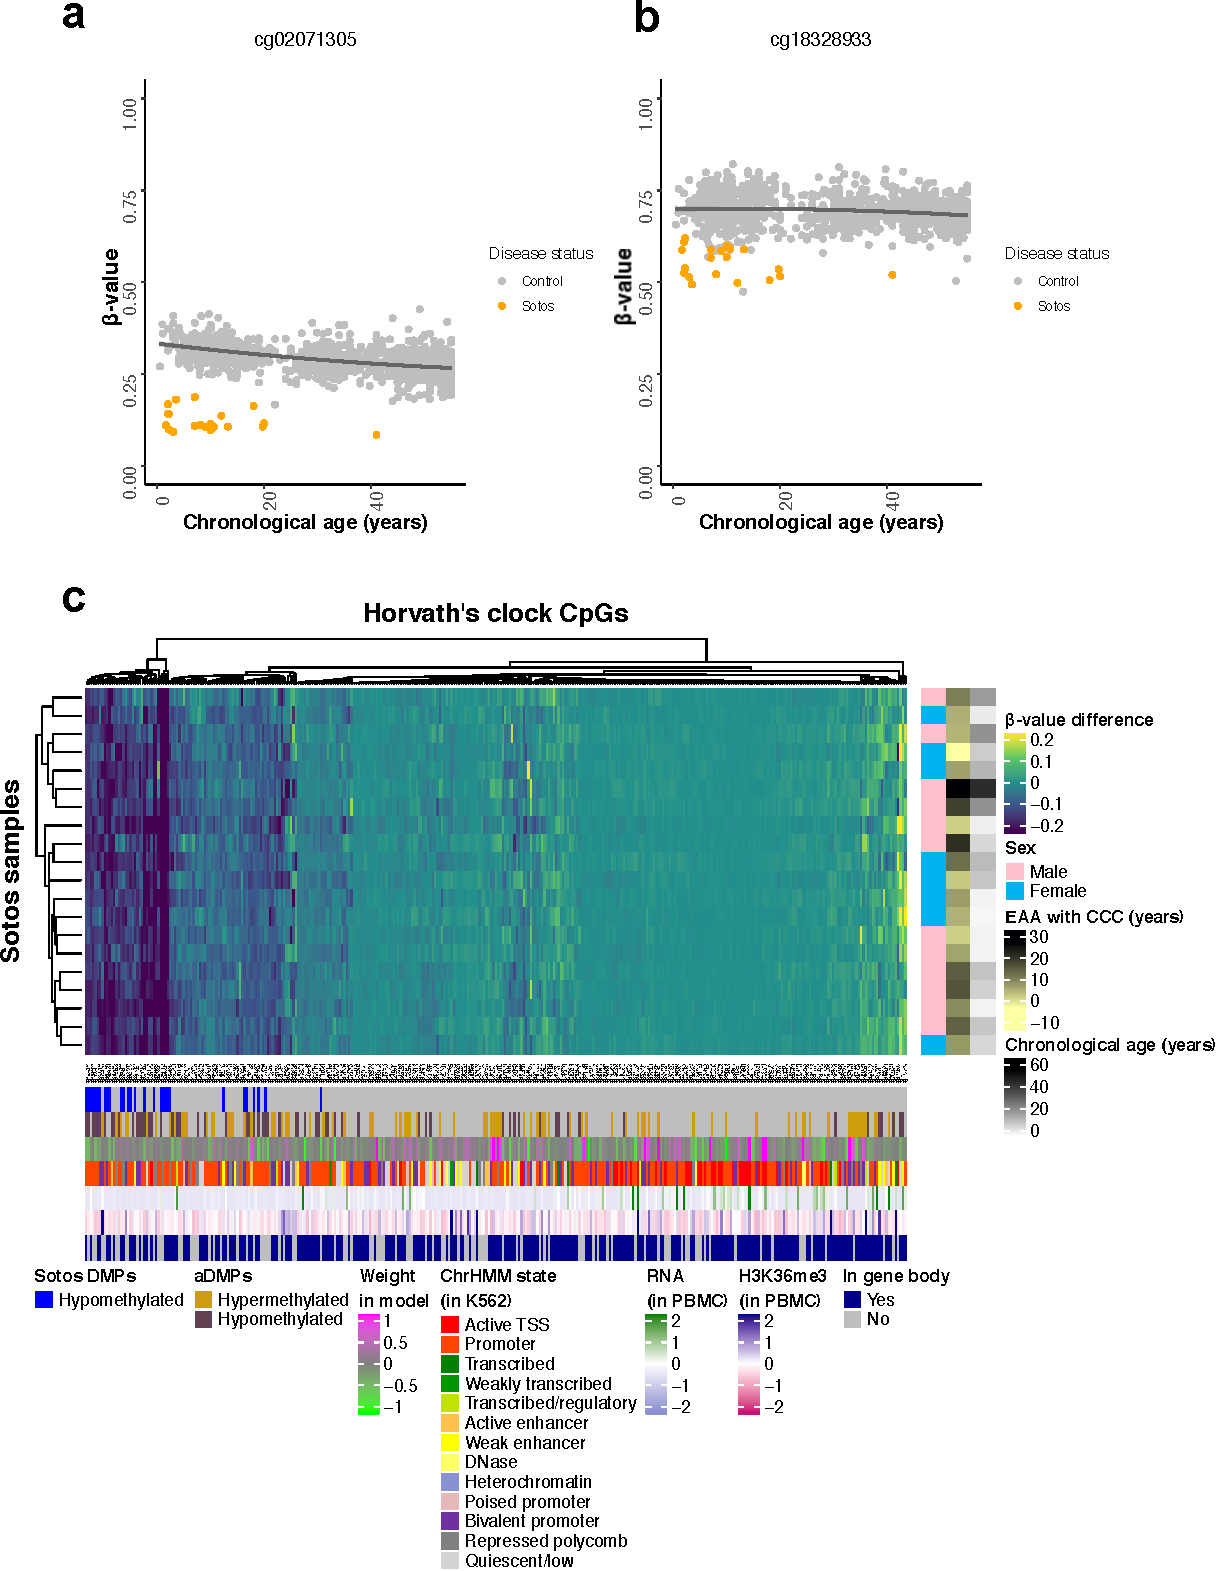
\includegraphics[width=1\textwidth]{C3_Fig6}
	\vspace*{1 mm}
	\caption[Landscape of Horvath's epigenetic clock CpGs in Sotos syndrome]{The landscape of Horvath's epigenetic clock CpG sites in Sotos syndrome. \textbf{a.} and \textbf{b.} DNA methylation ($\beta$-value) profiles for two of the clock CpG sites (cg02071305 and cg18328933). A linear model (displayed in dark grey, see equation~\ref{eq:3.4}) can be fixed to each CpG site to model the changes in $\beta$-value with chronological age in the controls (grey). Afterwards, the difference of the Sotos samples $\beta$-values (orange) with the controls can be estimated. \textbf{c.} Heatmap displaying the differential methylation patterns for Sotos samples (rows) when compared with controls in each one of the 353 epigenetic clock CpGs (columns). Hierarchical clustering was performed in both rows and columns. RNA refers to the `normalised RNA expression' (NRE). H3K36me3 refers to the H3K36me3 histone modification `normalised fold change' (NFC). aDMPs: differentially methylated positions during ageing. EAA: epigenetic age acceleration. CCC: cell composition correction. PBMC: peripheral blood mononuclear cells.}
	\label{fig:c3_fig6}
\end{figure}

\bigskip

I have demonstrated that the ageing process and Sotos syndrome share a subset of hypomethylated CpG sites that is characterised by an enrichment in enhancer features and a depletion of active transcription activity. This highlights the usefulness of \textbf{developmental disorders as a model to study the mechanisms that may drive the changes in the methylome with age}, since they permit stratification of the ageing DMPs into different functional categories that are associated with alterations in the function of specific genes and hence specific molecular components of the epigenetic ageing clock.

\smallskip

\section{Methylation Shannon entropy and the epigenetic clock} \label{s:3.5}

\smallskip

In section~\ref{s:2.1.5} I have discussed how Shannon entropy can be applied in the context of DNA methylation data in order to measure the genome-wide epigenetic information loss that happens during ageing. It is possible to apply a methodology similar to the one described in section~\ref{s:2.2.2} to compare the methylation Shannon entropy in healthy controls (0-55 years) and Sotos patients (i.e. using a linear model similar to equation~\ref{eq:2.16}, although in this case the dependent variable is the entropy value). This allows testing whether Sotos syndrome patients present genome-wide Shannon entropy acceleration i.e. deviations from the expected genome-wide Shannon entropy for their age. Despite detailed analysis, I did not find evidence that this was the case when looking genome-wide (p-value = 0.71, Fig.~\ref{fig:c3_fig7}a,b, Fig.~\ref{fig:sc3_fig9}a).

\begin{figure}[htbp!] 
	\centering    
	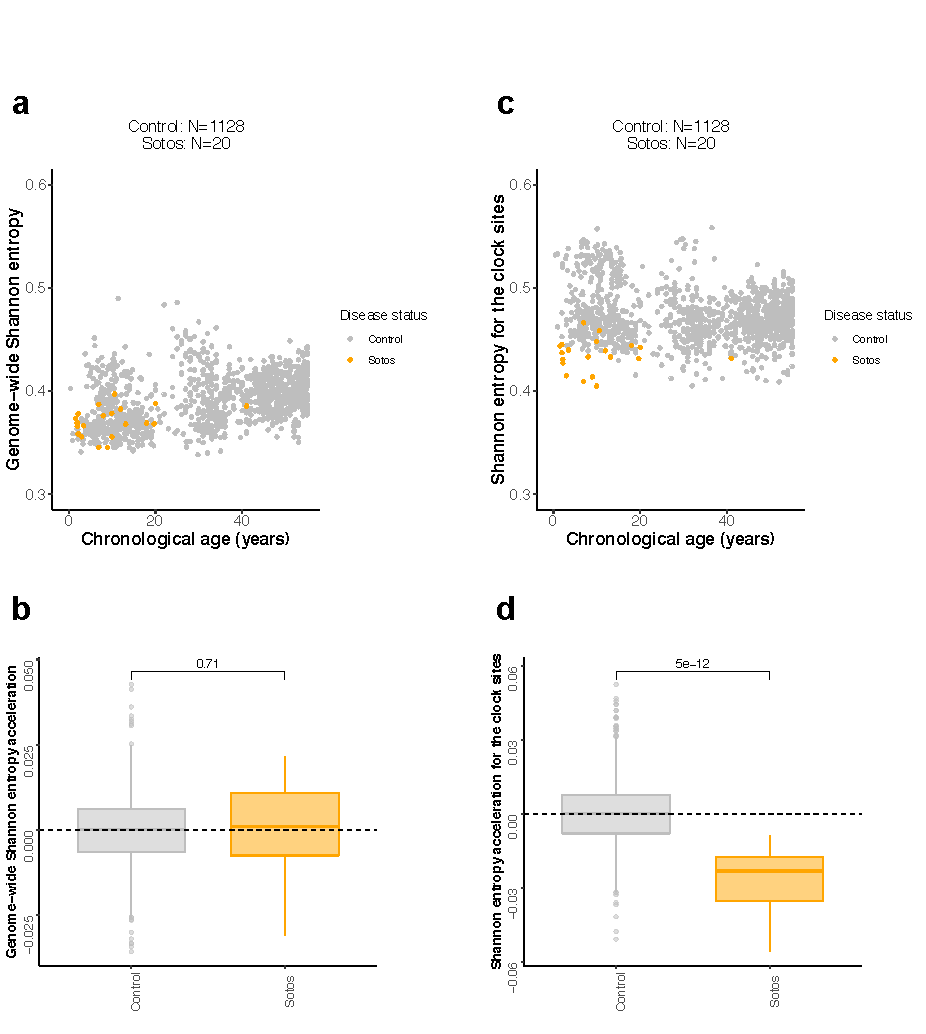
\includegraphics[width=1\textwidth]{C3_Fig7}
	\vspace*{1 mm}
	\caption[Methylation Shannon entropy during physiological ageing and in Sotos syndrome]{Analysis of methylation Shannon entropy during physiological ageing and in Sotos syndrome. \textbf{a.} Scatterplot showing the relation between genome-wide Shannon entropy (i.e. calculated using the methylation levels of all the CpG sites in the array) and chronological age of the samples for Sotos (orange) and healthy controls (grey). Each sample is represented by one point. \textbf{b.} Boxplots showing the distributions of genome-wide Shannon entropy acceleration (i.e. deviations from the expected genome-wide Shannon entropy for their age) for the control and Sotos samples. The p-value displayed on top of the boxplots was derived from a two-sided Wilcoxon’s test. \textbf{c.} As in a., but using the Shannon entropy calculated only for the 353 CpG sites in the Horvath's epigenetic clock. \textbf{d.} As in b., but using the Shannon entropy calculated only for the 353 CpG sites in the Horvath's epigenetic clock.}
	\label{fig:c3_fig7}
\end{figure}

\bigskip

When I considered only the 353 Horvath's epigenetic clock CpG sites for the entropy calculations, the picture was different. Shannon entropy for the 353 clock sites slightly decreased with age in the controls when I included all the batches, showing the opposite direction when compared with the genome-wide entropy (\acrshort{SCC} $= -0.1223$, p-value = 3.8166 $\cdot 10^{-5}$, Fig.~\ref{fig:c3_fig7}c). However, when I removed the `Europe' batch (which was an outlier even after pre-processing, Fig.~\ref{fig:sc3_fig10}), this trend was reversed and I observed a weak increase of clock Shannon entropy with age (\acrshort{SCC} $= 0.1048$, p-value = 8.6245 $\cdot 10^{-5}$). This shows that Shannon entropy calculations are very sensitive to batch effects, especially when considering a small number of CpG sites, and the results must be interpreted carefully, as already discussed in section~\ref{s:2.1.5}.

\bigskip

Interestingly, the mean Shannon entropy across all the control samples was higher in the epigenetic clock sites (mean = 0.4726, Fig.~\ref{fig:c3_fig7}c) with respect to the genome-wide entropy (mean = 0.3913, Fig.~\ref{fig:c3_fig7}a). Sotos syndrome patients displayed a lower clock Shannon entropy when compared with the control (p-value = 5.0449 $\cdot 10^{-12}$, Fig.~\ref{fig:c3_fig7}d, Fig.~\ref{fig:sc3_fig9}b), which is probably driven by the hypomethylation of the clock CpG sites. Furthermore, this highlights that the \textbf{Horvath's epigenetic clock sites could have slightly different characteristics in terms of the methylation entropy associated with them} when compared with the genome as a whole, something that to my knowledge has not been reported before.

\smallskip

\section{Discussion}

\smallskip

The epigenetic ageing clock has emerged as the most accurate biomarker of the ageing process and it seems to be a conserved property in mammalian genomes \citep{Horvath2018,Field2018}. However, it is still unknown whether the age-related DNA methylation changes measured are functional at all or whether they are related to some fundamental process of the biology of ageing. Developmental disorders in humans represent an interesting framework to look at the biological effects of mutations in genes that are fundamental for the integrity of the epigenetic landscape and other core processes, such as growth or neurodevelopment \citep{Aref-Eshghi2018,Bjornsson2015}. Therefore, using a reverse genetics approach, I aimed to identify genes that disrupt aspects of the behaviour of the epigenetic ageing clock in humans.

\bigskip

Most of the studies have looked at the epigenetic ageing clock using Horvath’s epigenetic clock \citep{Horvath2013}, and I decided to employ it as a tool to measure the epigenetic age of my samples. The results from the screen strongly suggest that Sotos syndrome accelerates epigenetic ageing. Sotos syndrome is caused by loss-of-function mutations in the NSD1 gene \citep{Choufani2015,Kurotaki2002}, which encodes a histone H3 lysine 36 (\acrshort{H3K36}) methyltransferase. This leads to a phenotype which can include pre-natal and post-natal overgrowth, facial gestalt, advanced bone age, developmental delay, higher cancer predisposition and, in some cases, heart defects \citep{Leventopoulos2009}. Remarkably, many of these characteristics could be interpreted as ageing-like, identifying \textbf{Sotos syndrome as a potential human model of accelerated physiological ageing}.

\bigskip

NSD1 catalyses the addition of either monomethyl (H3K36me) or dimethyl groups (H3K36me2) and indirectly regulates the levels of trimethylation (\acrshort{H3K36me3}) by altering the availability of the monomethyl and dimethyl substrates for the trimethylation enzymes (SETD2 in humans, whose mutations cause a `Sotos-like' overgrowth syndrome ) \citep{Wagner2012,Luscan2014}. H3K36 methylation has a complex role in the regulation of transcription \citep{Wagner2012} and has been shown to regulate nutrient stress response in yeast \citep{McDaniel2017}. Moreover, experiments in model organisms (yeast and worm) have demonstrated that \textbf{mutations in H3K36 methyltranferases decrease lifespan and, remarkably, mutations in H3K36 demethylases increase it} \citep{Ni2012,Sen2015,Pu2015}.

\bigskip

In humans, DNA methylation patterns are established and maintained by three conserved enzymes: the maintenance DNA methyltransferase DNMT1 and the \textit{de novo} DNA methyltransferases DNMT3A and DNMT3B \citep{Schubeler2015}. Both DNMT3A and DNMT3B contain PWWP domains that can read the H3K36me3 histone mark \citep{Dhayalan2010,Baubec2015}. Therefore, the H3K36 methylation landscape can influence DNA methylation levels in specific genomic regions through the recruitment of the \textit{de novo} DNA methyltransferases. Mutations in the PWWP domain of DNMT3A impair its binding to H3K36me2 and H3K36me3 and cause an undergrowth disorder in humans (microcephalic dwarfism) \citep{Heyn2019}. This redirects DNMT3A, which is normally targeted to H3K36me2 and H3K36me3 throughout the genome, to DNA methylation valleys (\acrshort{DMV}s, a.k.a DNA methylation canyons), which become hypermethylated \citep{Heyn2019}; a phenomenon that also seems to happen during physiological ageing in humans \citep{Rakyan2010,Teschendorff2010,Slieker2016} and mice \citep{Cole2017}. DMVs are hypomethylated domains conserved across cell types and species, often associated with Polycomb-regulated developmental genes and marked by bivalent chromatin (with \acrshort{H3K27me3} and \acrshort{H3K4me3}) \citep{Xie2013,Long2013,Jeong2013,Li2018}. Therefore, I suggest a model (Fig.~\ref{fig:c3_fig8}) where the \textbf{reduction in the levels of H3K36me2 and/or H3K36me3, caused by a proposed decrease in H3K36 methylation maintenance during ageing or NSD1 function in Sotos syndrome, could lead to hypomethylation in many genomic regions (because DNMT3A is recruited less efficiently) and hypermethylation in DMVs (because of the higher availability of DNMT3A)}. Indeed, I observe enrichment for categories such as `bivalent promoter' or `repressed polycomb' in the hypermethylated DMPs in Sotos and ageing (Fig.~\ref{fig:sc3_fig4}), which is also supported by higher levels of Polycomb Repressing Complex 2 (\acrshort{PRC2}, represented by EZH2) and H3K27me3, the mark deposited by PRC2 (Fig.~\ref{fig:sc3_fig5}).This is also consistent with the results obtained for the epigenetic mitotic clock \citep{Yang2016}, where I observe a trend towards increased hypermethylation of Polycomb-bound regions in Sotos patients. Furthermore, it is worth mentioning that a mechanistic link between PRC2 recruitment and H3K36me3 has also been unravelled via the Tudor domains of some polycomb-like proteins \citep{Cai2013,Li2017}.

\begin{figure}[htbp!] 
	\centering    
	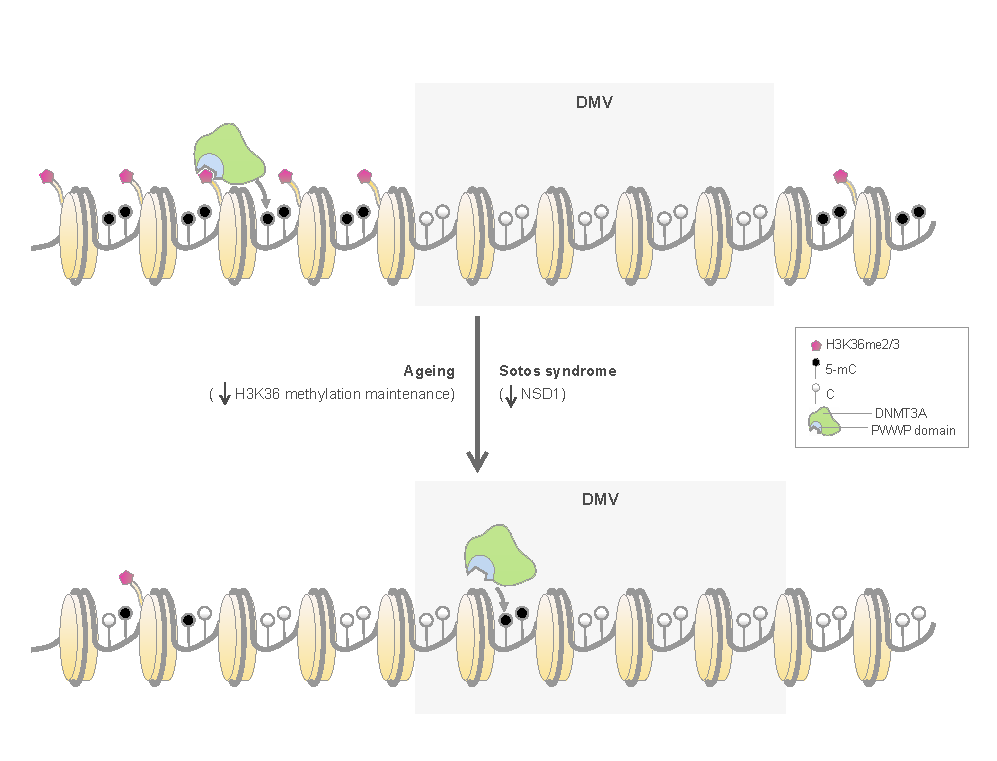
\includegraphics[width=1\textwidth]{C3_Fig8}
	\vspace*{1 mm}
	\caption[Proposed model that highlights the role of H3K36 methylation maintenance on epigenetic ageing]{Proposed model that highlights the role of H3K36 methylation maintenance on epigenetic ageing. The H3K36me2/3 mark allows recruiting \textit{de novo} DNA methyltransferases DNMT3A (in green) and DNMT3B (not shown) through their PWWP domain (in blue) to different genomic regions (such as gene bodies or pericentric heterochromatin) \citep{Baubec2015,Chantalat2011,Chen2004}, which leads to the methylation of the cytosines in the DNA of these regions (\acrshort{5mC}, black lollipops). On the contrary, DNA methylation valleys (\acrshort{DMV}s) are conserved genomic regions that are normally found hypomethylated and associated with Polycomb-regulated developmental genes \citep{Xie2013,Long2013,Jeong2013,Li2018}. During ageing, the H3K36 methylation machinery could become less efficient at maintaining the H3K36me2/3 landscape. This would lead to a relocation of \textit{de novo} DNA methyltransferases from their original \textit{genomic reservoirs} (which would become hypomethylated) to other non-specific regions such as DMVs (which would become hypermethylated and potentially lose their normal boundaries), with functional consequences for the tissues. This is also partially observed in patients with Sotos syndrome, where mutations in NSD1 potentially affect H3K36me2/3 patterns and accelerate the epigenetic ageing clock as measured with the Horvath's model \citep{Horvath2013}. Given that DNMT3B is enriched in the gene bodies of highly transcribed genes \citep{Baubec2015} and that I found these regions depleted in the differential methylation analysis, I hypothesise that the hypermethylation of DMVs could be mainly driven by DNMT3A instead. However, it is important to mention that my analysis does not discard a role of DNMT3B during epigenetic ageing.}
	\label{fig:c3_fig8}
\end{figure}

\bigskip

A recent preprint has shown that loss-of-function mutations in DNMT3A, which cause Tatton-Brown-Rahman overgrowth syndrome, also lead to a higher ticking rate of the epigenetic ageing clock \citep{Jeffries2018}. They also report positive epigenetic age acceleration in Sotos syndrome and negative acceleration in Kabuki syndrome, consistent with my results. Furthermore, they observe a DNA methylation signature in the DNMT3A mutants characterised by widespread hypomethylation, with a modest enrichment of DMPs in regions upstream of the transcription start site, shores and enhancers \citep{Jeffries2018}, which I also detect in the `Hypo-Hypo DMPs' (those that become hypomethylated both during physiological ageing and in Sotos). Therefore, \textbf{the hypomethylation observed in the `Hypo-Hypo DMPs' is consistent with a reduced methylation activity of DNMT3A}, which in my analysis could be a consequence of the decreased recruitment of DNMT3A to genomic regions that have lost H3K36 methylation (Fig.~\ref{fig:c3_fig8}).

\bigskip

Interestingly, H3K36me3 is required for the selective binding of the \textit{de novo} DNA methyltransferase DNMT3B to the bodies of highly transcribed genes \citep{Baubec2015}. Furthermore, DNMT3B loss reduces gene-body methylation, which leads to intragenic spurious transcription (a.k.a cryptic transcription) \citep{Neri2017}. An increase in this so-called cryptic transcription seems to be a conserved feature of the ageing process \citep{Sen2015}. Therefore, the changes observed in the `Hypo-Hypo DMPs' could theoretically be a consequence of the loss of H3K36me3 and the concomitant inability of DNMT3B to be recruited to gene bodies. However, the `Hypo-Hypo DMPs' were depleted for H3K36me3, active transcription and gene bodies when compared with the rest of the probes in the array (Fig.~\ref{fig:c3_fig5}b-d), prompting me to suggest that the DNA methylation changes observed are likely mediated by DNMT3A instead (Fig.~\ref{fig:c3_fig8}). Nevertheless, it is worth mentioning that the different biological replicates for the blood H3K36me3 ChIP-seq datasets were quite heterogeneous and that the absolute difference in the case of the hypomethylated Sotos DMPs, although significant due to the big sample sizes, is quite small. Thus, I cannot exclude the existence of this mechanism during human ageing and an exhaustive study on the prevalence of cryptic transcription in humans and its relation to the ageing methylome should be carried out.

\bigskip

H3K36me3 has also been shown to guide deposition of the N$^6$-methyladenosine \acrshort{mRNA} modification (\acrshort{m$^6$A}), an important post-transcriptional mechanism of gene regulation \citep{Huang2019}. Interestingly, a decrease in overall \acrshort{m$^6$A} during human ageing has been previously reported in \acrshort{PBMC}s \citep{Min2018}, suggesting another biological route through which an alteration of the H3K36 methylation landscape could have functional consequences for the organism.

\bigskip

Because of the way that the Horvath epigenetic clock was trained \citep{Horvath2013}, it is likely that its constituent 353 CpG sites are a \textbf{low-dimensional representation of the different genome-wide processes that are eroding the epigenome with age}. My analysis has shown that these 353 CpG sites are characterised by a higher Shannon entropy when compared with the rest of the genome, which is dramatically decreased in the case of Sotos patients. This could be related to the fact that Horvath's clock CpGs are enriched in regions of bivalent chromatin (marked by H3K27me3 and H3K4me3), conferring a more dynamic or plastic regulatory state with levels of DNA methylation deviated from the collapsed states of 0 or 1. Interestingly, EZH2 (part of Polycomb Repressing Complex 2, responsible for H3K27 methylation) is an interacting partner of DNMT3A and NSD1, with mutations in NSD1 affecting the genome-wide levels of H3K27me3 \citep{Streubel2018}. Furthermore, Kabuki syndrome was weakly identified in my screen as having an epigenome younger than expected, which could be related to the fact that they show post-natal dwarfism \citep{Aref-Eshghi2017,Butcher2017}. Kabuki syndrome is caused by loss-of-function mutations in KMT2D \citep{Aref-Eshghi2017,Butcher2017}, a major mammalian H3K4 mono-methyltransferase \citep{Froimchuk2017}. Additionally, H3K27me3 and H3K4me3 levels can affect lifespan in model organisms \citep{Sen2016}. It will be interesting to test whether bivalent chromatin is a general feature of multi-tissue epigenetic ageing clocks.

\bigskip

Thus, \textbf{DNMT3A, NSD1 and the machinery in control of bivalent chromatin (such as EZH2 and KMT2D) contribute to an emerging picture on how the mammalian epigenome is regulated during ageing}, which could open new avenues for anti-ageing drug development. Mutations in these proteins lead to different developmental disorders with impaired growth defects \citep{Bjornsson2015}, with DNMT3A, NSD1 and potentially KMT2D also affecting epigenetic ageing. Interestingly, EZH2 mutations (which cause Weaver syndrome, Table~\ref{table:c3_table1}) do not seem to affect the epigenetic clock in my screen. However, this syndrome has the smallest number of samples ($N=7$) and this could limit the power to detect any changes.

\bigskip

My screen has also revealed that \textbf{Rett syndrome and fragile X syndrome (\acrshort{FXS}) could potentially have an accelerated epigenetic age}. It is worth noting that FXS is caused by an expansion of the CGG trinucleotide repeat located in the 5' \acrshort{UTR} of the FMR1 gene \citep{Schenkel2016}. Interestingly, Huntington's disease, caused by a trinucleotide repeat expansion of CAG, has also been shown to accelerate epigenetic ageing of human brain \citep{Horvath2016a}, pointing towards trinucleotide repeat instability as an interesting molecular mechanism to look at from an ageing perspective. It is important to notice that the conclusions for Rett syndrome, FXS and Kabuki syndrome were very dependent on the age range used in the healthy control (Fig.~\ref{fig:sc3_fig2}) and these results must therefore be treated with caution.

\bigskip

This study has several \textbf{limitations that I tried to address in the best possible way}. First of all, given that DNA methylation data for patients with developmental disorders is relatively rare, some of the sample sizes were quite small. It is thus possible that some of the other developmental disorders assessed are epigenetically accelerated but I lack the power to detect this. Furthermore, people with the disorders tend to get sampled when they are young i.e. before reproductive age. Horvath's clock adjusts for the different rates of change in the DNA methylation levels of the clock CpGs before and after adult/reproductive age (20 years in humans) \citep{Horvath2013}, but this could still have an effect on the predictions, especially if the control is not properly age-matched. My solution was to discard those developmental disorders with less than 5 samples and I required them to have at least 2 samples with an age $\geq$ 20 years, which reduced the list of final disorders included to the ones listed in Table~\ref{table:c3_table1}. 

\bigskip

Future studies should increase the sample size and follow the patients during their entire lifespan in order to confirm these findings. Furthermore, it would be interesting to identify mutations that affect, besides the mean, the variance of epigenetic age acceleration, since changes in methylation variability at single CpG sites with age have been associated with fundamental ageing mechanisms \citep{Slieker2016}. Finally, testing the influence of H3K36 methylation on the epigenetic clock and lifespan in mice will provide deeper mechanistic insights.

\smallskip

\section{Additional methods} \label{s:3.7}

\subsection*{Sample generation and annotation}

I collected DNA methylation data generated with the Illumina Infinium HumanMethylation450 BeadChip (450K array) from human blood. In the case of the developmental disorder samples, I combined public data with data generated in-house by my collaborators in Canada (Table~\ref{table:s2_table1}, Fig.~\ref{fig:sc3_fig1}). The wet-lab protocols used in the public datasets can be found in their respective GEO repositories. DNA methylation data from my Canadian collaborators was generated according to the manufacturer's protocol \citep{Research,Illumina2015}.

\bigskip

Basic metadata (including the chronological age) was also stored. All the mutations in the developmental disorder samples were manually curated using Variant Effect Predictor \citep{McLaren2016} in the GRCh37 (\acrshort{hg19}) human genome assembly. Those samples with a variant of unknown significance that had the characteristic DNA methylation signature of the disease were also included (they are labelled as `YES\_predicted' in Fig.~\ref{fig:sc3_fig1}). In the case of fragile X syndrome (\acrshort{FXS}), only male samples with full mutation (>200 repeats) \citep{Schenkel2016} were included in the final screen. As a consequence, only samples with a clear molecular and clinical diagnosis were kept for the final screen.

\subsection*{Identifying differentially methylated positions in Sotos syndrome} 

Following a strategy similar to the one outlined in section~\ref{s:2.1.4}, I identified those array probes that were differentially methylated in patients with Sotos syndrome. I compared the Sotos samples (N=20) against the internal control samples (N=51) from the same dataset (GSE74432) \citep{Choufani2015}, fitting the following linear model to each one of the array probes:

\begin{align} \label{eq:3.1}
Beta \sim Disease\_status + Age + Sex+ Gran + CD4T + CD8T + B + Mono + NK + PC1 + ... + PC17
\end{align} 

where $Beta$ is the $\beta$-value for the array probe being evaluated; $Disease\_status$ indicates whether a sample comes from a healthy individual (0) or a Sotos syndrome patient (1); $Age$ is the chronological age (in years) of the samples; $Sex$ encodes for the sex of the samples (0/1); $Gran$, $CD4T$, $CD8T$, $B$, $Mono$ and $NK$ are the cell type proportions from the samples as calculated with my cell-type deconvolution strategy and $PCN$ is the $N$th principal component that captures technical variance and accounts for potential batch effects (see section~\ref{s:2.2.3} for more details).

\bigskip

P-values and regression coefficients were extracted for the $Disease\_status$ covariate. I selected as my final Sotos DMPs those CpG probes that survived the analysis after Bonferroni multiple testing correction with a significance level of $\alpha=0.01$. 

\subsection*{(Epi)genomic annotation of the CpG sites}

Different (epi)genomic features were extracted for the CpG sites of interest. All the data were mapped to the \textit{hg19} assembly of the human genome.
The \textbf{continuous features} were calculated by extracting the mean value in a window of $\pm$ 200 bp from the CpG site coordinate using the \textit{pyBigWig} package \citep{Richter}. I chose this window value based on the methylation correlation observed between neighbouring CpG sites in previous studies \citep{Zhang2015}. The continuous features included (Fig.~\ref{fig:sc3_fig11}):

\begin{itemize}
	
	\item ChIP-seq data from ENCODE (histone modifications from peripheral blood mononuclear cells or \acrshort{PBMC}; EZH2, as a marker of Polycomb Repressing Complex 2 binding, from B cells; RNF2, as a marker of Polycomb Repressing Complex 1 binding, from the K562 cell line). I obtained Z-scores (using the \textit{scale} function in R) for the values of `fold change over control' as calculated in ENCODE \citep{Consortium2012}. When needed, biological replicates of the same feature were aggregated by taking the mean of the Z-scores in order to obtain the `normalised fold change' (\acrshort{NFC}).
	
	\item ChIP-seq data for LaminB1 (GSM1289416, quantified as `normalised read counts' or \acrshort{NRC}) and \acrshort{Repli-seq} data for replication timing (GSM923447, quantified as `wavelet-transformed signals' or \acrshort{WTS}). I used the same data from the IMR90 cell line as in \citep{Zhou2018}.
	
	\item Total RNA-seq data (\acrshort{rRNA} depleted, from PBMC) from ENCODE. I calculated Z-scores after aggregating the `signal of unique reads' (\textit{\acrshort{sur}}) for both strands (+ and - ) in the following manner:
	
	\begin{align}
	RNA_i = \log_2(1 + sur_{i+} + sur_{i-})
	\end{align}
	
	where $RNA_i$ represents the RNA signal (that then needs to be scaled to obtain the `normalised RNA expression' or \acrshort{NRE}) for the $i$th CpG site.
	
\end{itemize}

The \textbf{categorical features} were obtained by looking at the overlap (using the \textit{pybedtools} package) \citep{Quinlan2011} of the CpG sites with the following:

\begin{itemize}
	
	\item Gene bodies, from protein-coding genes as defined in the basic gene annotation of GENCODE release 29 \citep{Frankish2018}.
	
	\item CpG islands (\acrshort{CGI}s) were obtained from the UCSC Genome Browser \citep{Bock2007}. Shores were defined as regions 0 to 2 kb away from CGIs in both directions and shelves as regions 2 to 4 kb away from CGIs in both directions as previously described \citep{Zhang2015,Martin-Herranz2017a}.
	
	\item Chromatin states were obtained from the K562 cell line in the Roadmap Epigenomics Project (based on imputed data, 25 states, 12 marks) \citep{Consortium}. A visualisation for the association between chromatin marks and chromatin states can be found in \citep{Consortiuma}. When needed for visualisation purposes, the 25 states were manually collapsed to a lower number of them.
	
\end{itemize}

I compared the different genomic features for each one of the subsets of CpG sites (hypomethylated aDMPs, hypomethylated Sotos DMPs, etc.) against a control set. This control set was composed of all the probes from the background set from which I removed the subset that I was testing. In the case of the comparisons against the 353 Horvath clock CpG sites, a background set of the 21368 (21K) CpG probes used to train the original Horvath model \citep{Horvath2013} was used. In the case of the genome-wide comparisons for ageing and Sotos syndrome, a background set containing all 428266 probes that passed my pre-processing pipeline was used (see section~\ref{s:2.1.2}).

\bigskip

For each continuous feature, the feature score distributions for a given subset of CpG sites and the control set were compared using the non-parametric two-sided Wilcoxon's test. For each categorical feature, I first created a $2x2$ contingency table, with the two variables indicating whether a given CpG site overlaps with the categorical feature under consideration (Yes/No) and whether the CpG site is in the subset (e.g. hypomethylated aDMPs) being considered (Yes/No). Using Fisher's exact test (as implemented in the \textit{fisher.test} function in R) I calculated the p-value and the odds ratio (\acrshort{OR}), which allows determining whether the categorical feature under consideration is enriched in the CpGs subset. 

\subsection*{Differences in the epigenetic clock CpGs $\beta$-values for Sotos syndrome}

To compare the $\beta$-values of the Horvath clock CpG sites between the healthy samples and Sotos samples I fitted the following linear model to each array probe from the Horvath's epigenetic clock (353 in total) in the healthy individuals samples (Fig.~\ref{fig:c3_fig6}a,b):

\begin{align} \label{eq:3.4}
Beta \sim Age+Age^2+Sex+Gran+CD4T+CD8T+B+Mono+NK+PC1+... +PC17
\end{align}

where $Beta$ is the $\beta$-value for the clock array probe being evaluated; $Age$ is the chronological age (in years) of the samples; $Sex$ encodes for the sex of the samples (0/1); $Gran$, $CD4T$, $CD8T$, $B$, $Mono$ and $NK$ are the cell type proportions from the samples as calculated with my cell-type deconvolution strategy and $PCN$ is the $N$th principal component that captures technical variance and accounts for potential batch effects (see section~\ref{s:2.2.3} for more details). The $Age^2$ covariate allows accounting for non-linear relationships between chronological age and the $\beta$-values.

\bigskip

Finally, I calculated the difference between the $\beta$-values in Sotos samples and the predictions from the models in equation~\ref{eq:3.4} and displayed these differences in an annotated heatmap (Fig.~\ref{fig:c3_fig6}c).   


%!TEX root = ../thesis.tex
%*******************************************************************************
%****************************** Fourth Chapter *********************************
%*******************************************************************************

\chapter{Technological aspects} \label{c:4}

\ifpdf
	\graphicspath{{Chapter4/Figs/pdf/}}
\else
	\graphicspath{{Chapter4/Figs/svg/}}
\fi

\epigraph{`It is perfectly true, as the philosophers say, that life must be understood backwards. But they forget the other proposition, that it must be lived forwards.'}{Søren \citet{Kierkegaard1843}}

\subsection*{Declaration} 

\footnotesize

The content of this chapter was joint work with Tom Stubbs, with whom I designed and developed cuRRBS. Nevertheless, almost all the text, code and plots here presented were produced by myself. Additionally, I would like to recognise the contributions of Janet M. Thornton and Wolf Reik (who helped designing the study), Antonio J. M. Ribeiro (who implemented the last version of cuRRBS to make it more computationally efficient) and Felix Krueger (who processed the RRBS datasets). All of them also helped in the revision of the final text. This work has been published in the journal \textit{Nucleic Acids Research} \citep{Martin-Herranz2017a}.

\normalsize

\section{Background} \label{s:4.1}

\smallskip

With the advent of next-generation sequencing, scientists are studying the biology of life at unprecedented resolution \citep{Shendure2008}. Unfortunately, owing to the large size of many commonly studied genomes (human, mouse and tobacco plant for example are all > 2.5 \acrshort{Gbp} in size) \citep{Consortium2001,Consortium2002,Sierro2014}, it is often still prohibitively expensive to conduct whole genome sequencing at high coverage. This creates a trade-off that negatively impacts the number of replicates that can be included and, therefore, it challenges the statistical power and the reproducibility of the studies \citep{Fumagalli2013,Wu2015}. This is true in particular for \acrshort{DNA} methylation, where differentially methylated regions ( \acrshort{DMRs}) are typically called by identifying changes as small as $10\%$ and where $70-80\%$ of the reads of Whole Genome Bisulfite Sequencing (\acrshort{WGBS}) methods contain little to no relevant information on the DNA methylation status \citep{Ziller2013}.

\bigskip

To address these cost inefficiencies, many methods have been developed to \textbf{reduce the number of genomic fragments that need to be sequenced} for a given biological system \citep{Plongthongkum2014,Suzuki2013,Yong2016,Kurdyukov2016,Kacmarczyk2018}. These methods can be broadly split into those that positively select for genomic fragments of interest and those that deplete for fragments that are not of interest. Positive selection-based methods involve the sites of interest being enriched from the background. This usually occurs through pull-down of these sites via an antibody (e.g. anti-\acrshort{5mC} antibody) \citep{Taiwo2012}, a recombinant binding protein (e.g. methyl-\acrshort{CpG}-binding domains or \acrshort{MBD}) \citep{Brinkman2010}, covalent biotin tagging \citep{Kriukiene2013}, capture probes/baits for the sites of interest \citep{Ivanov2013,Allum2015,Cheung2017}, array-based approaches (e.g. \acrshort{27K}, \acrshort{450K} and \acrshort{EPIC} arrays in human) \citep{Bibikova2009,Bibikova2011,Pidsley2016,Hodges2009} or \acrshort{PCR}-based approaches \citep{Deng2009,Diep2012,Komori2011,Paul2014,Bernstein2015,Yang2015}. These methods have many limitations, including enrichment biases, complex protocols and difficulties in quantification \citep{Suzuki2013,Yong2016}.

\bigskip 

Current evidence shows that depletion-based methods do not have enrichment biases, tend to be simpler and are more readily quantifiable \citep{Suzuki2013,Kurdyukov2016}. The most common depletion-based approaches use restriction enzymes to exploit the fact that the nucleotide composition in a given genome is non-random and that the fragment lengths produced from a given digestion will thus reflect this \citep{Cedar1979,Cohen-Karni2011,Bystrykh2013,Martinez-Arguelles2014,Yu2004}. In the case of 5-methylcytosine (5mC), the most common depletion-based method is Reduced Representation Bisulfite Sequencing (\acrshort{RRBS}) using the methylation-insensitive restriction enzyme MspI (with the recognition sequence C|CGG) \citep{Meissner2008,Boyle2012}, although enzymes such as BglII \citep{Meissner2005}, XmaI \citep{Tanas2017}, Taq$^\alpha$I \citep{Lee2014,Lim2016}, MspJI \citep{Huang2013} , ApeKI \citep{Wang2013}, HpyCH4IV or HpaII \citep{Kirschner2016} have also been used. RRBS has proven extremely useful for cost-effective, global studies of DNA methylation \citep{Stubbs2017,Meissner2008,Lee2014,Gu2010}, capturing around $10\%$ of CpG sites within mammalian genomes but with up to a 30-fold reduction in the number of fragments sequenced in comparison to WGBS \citep{Smith2009}. 

\bigskip

In the context of epigenetic clocks, most studies have used methylation arrays in humans \citep{Koch2011,Hannum2013,Horvath2013} and MspI-based RRBS in mice, dogs and wolves \citep{Thompson2017,Stubbs2017,Petkovich2017,Thompson2018,Meer2018}. The utility of the MspI-based RRBS approach is limited to a specific subset of CpG sites in the genome, mainly found within CpG islands and promoters \citep{Meissner2008}. Nevertheless, it is known that many age-related changes in the methylome occur in other genomic regions (such as enhancers) \citep{Cole2017,Slieker2016,Slieker2018,Martin-Herranz2019a}, and current technologies could be biasing our discoveries. Furthermore, epigenetic clocks could be used in the near future to perform high-throughput screenings of anti-ageing drugs or employed as ageing biomarkers in clinical trials \citep{Horvath2018a}. However, the current assay costs could preclude the use of epigenetic clocks in this context.

\bigskip 

Given that restriction enzyme-based approaches are versatile and simple, we developed a new computational method called \textbf{customised Reduced Representation Bisulfite Sequencing} (\acrshort{cuRRBS}), which allows researchers to optimise the RRBS protocol for a specific experiment. cuRRBS generalises the problem of genomic enrichment with restriction enzymes by allowing the user to define both the genome and the particular sites of interest, before outputting the optimal enzyme combinations and size ranges to target these sites. In addition, cuRRBS provides the user with a variety of metrics to compare the various suggested protocols, including an estimate of the fold-reduction in sequencing costs compared to WGBS and a robustness value to assess the impact of experimental error in the size selection step.

\bigskip

Here, we have tested the enrichment ability of cuRRBS in several biological systems (including the Horvath epigenetic clock), with sites in both CpG and \acrshort{CHG} contexts and multiple species, to showcase the generalisability and utility of the software \citep{Horvath2013,Hanna2016,Milagre2017,Kawakatsu2016,Maurano2015,LevMaor2015,Domcke2015}. In addition, we take advantage of two recently published independent RRBS datasets to demonstrate the accuracy of the software predictions in both single and double enzyme experimental settings \citep{Tanas2017,Lim2016}. We hope that cuRRBS will be useful as a tool for designing cost-effective, genome-wide studies in the future, to help in the development of new epigenetic-based predictors and to validate previous results from whole genome approaches in a simple, cheap and timely fashion.

\smallskip

\section{Restriction enzyme digestion as a tool for genomic enrichment}

\smallskip

Restriction enzymes represent an incredibly effective tool for the enrichment of certain sites of interest in a genome. This is possible due to the wide variety of motifs that commercially-available restriction enzymes can recognise (Fig.~\ref{fig:c4_fig1}) combined with the non-random nature of the genome composition itself. Fig.~\ref{fig:c4_fig1} highlights that this motif diversity is driven both by the sequence composition (\acrshort{GC content}) and the length of the recognition sequence. Thus, \textbf{different restriction enzymes will generate different fragment length distributions}, dependent upon how frequently their recognition site is present in a given genome (Fig.~\ref{fig:c4_fig2}a, Fig.~\ref{fig:sc4_fig1}).

\vspace{3.5mm}


\begin{figure}[htbp!] 
	\centering    
	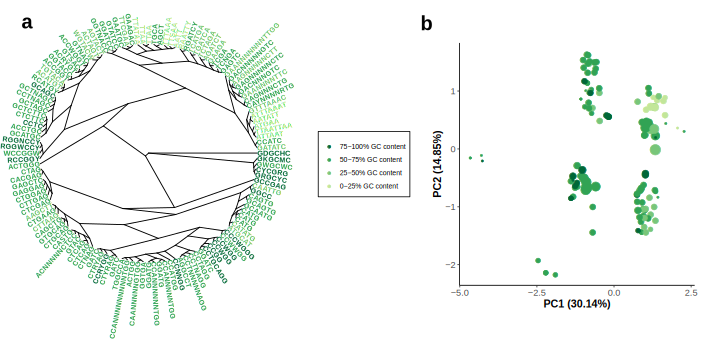
\includegraphics[width=1.0\textwidth]{C4_Fig1}
	\vspace*{1mm}
	\caption[The landscape of restriction enzyme motifs]{The landscape of restriction enzyme motifs. \textbf{a.} Phylogenetic analysis of the motifs that are recognised by the different commercially-available restriction enzymes which are insensitive to CpG methylation. Each sequence represents a different isoschizomer family considered in this study. A neighbour-joining method was used to construct the tree. Motifs with different GC content are shown with different colours. \textbf{b.} Principal component analysis (\acrshort{PCA}) performed on the matrix of pairwise distances from the aligned motifs. Each circle represents a different motif. The coordinates of the different motifs on the first two principal components are plotted on the x- and y-axes. Motifs with different GC content are shown with different colours (same as in a.) and the motif length is represented by the diameter of the circle.}
	\label{fig:c4_fig1}
\end{figure}


\begin{figure}[htbp!] 
	\centering    
	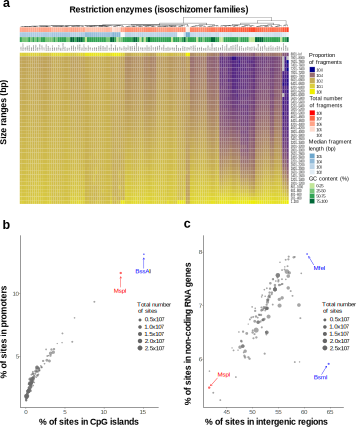
\includegraphics[scale=1.4]{C4_Fig2}
	\vspace*{3mm}
	\caption[Restriction enzyme digestion as a tool for genomic enrichment]{Restriction enzyme digestion as a tool for genomic enrichment. \textbf{a.} Heatmap showing the fragment length distributions generated by different restriction enzymes in the human genome (\acrshort{hg38}). Each column represents the distribution for an isoschizomer family of restriction enzymes that contains at least one member which is methylation-insensitive in a CpG context. The distributions are binned in size ranges of 200 \acrshort{bp}, ordered as they would appear in an electrophoretic gel. Additional row annotations on top of the heatmap contain information regarding the total number of fragments (in red) and the median fragment length (in blue) produced by each in silico digestion, together with the GC content of the recognition motif in the isoschizomer family (in green). Legend is displayed on the right hand side. \textbf{b.} Scatterplot showing the percentage of cleavage sites from different restriction enzymes that overlaps with CpG islands (x-axis) and promoters (y-axis) in the human genome (hg38). The size of the circles represents the total number of cleavage sites generated by each enzyme. The enzymes MspI and BssAI are highlighted in red and blue respectively. Legend is displayed on the right hand side. \textbf{c.} Scatterplot showing the percentage of cleavage sites from different restriction enzymes that overlaps with intergenic regions (x-axis) and non-coding \acrshort{RNA} genes (y-axis) in the human genome (hg38). The size of the circles represents the total number of cleavage sites generated by each enzyme. The enzyme MspI is highlighted in red. The enzymes BsmI and MfeI are both highlighted in blue. Legend is displayed on the right hand side.}
	\label{fig:c4_fig2}
\end{figure}

\bigskip

In DNA methylation studies the most common application is the use of MspI (cutting at C|CGG) in RRBS (Reduced Representation Bisulfite Sequencing), which is used to enrich for CG dinucleotides (CpGs) contained in promoters and CpG islands \citep{Meissner2008} (Fig.~\ref{fig:c4_fig2}b). However, \textbf{in many cases, MspI is by no means the most effective restriction enzyme} that could be used. For instance, MspI would be a poor restriction enzyme to choose for the enrichment of CpGs found in intergenic regions or non-coding RNA genes in the human genome, which would be far better enriched for using BsmI or MfeI respectively (Fig.~\ref{fig:c4_fig2}c). In fact, it turns out that across many genomic features MspI is rarely the most optimal methylation-insensitive restriction enzyme (Fig.~\ref{fig:sc4_fig2}). 

\bigskip

Previous studies have tested the potential of other restriction enzymes and enzyme combinations to expand the range of CpG sites that can be targeted in a genome \citep{Cedar1979,Bystrykh2013,Martinez-Arguelles2014,Yu2004,Tanas2017,Lee2014,Wang2013,Kirschner2016}. However, to our knowledge, there is currently no computational method that systematically explores the capacity of all commercially-available restriction enzymes to generate `personalised' reduced-representations of the genome whilst minimising the experimental cost (Fig.~\ref{fig:sc4_fig3}).

\smallskip

\section{cuRRBS: customised Reduced Representation Bisulfite Sequencing}

\smallskip

We have developed a novel computational method (cuRRBS) that \textbf{determines the optimal combination of restriction enzymes and size range to enrich for any given set of sites of interest in any genome}. In other words, by modifying two of the steps in the original RRBS protocol (Fig.~\ref{fig:c4_fig3}a), cuRRBS generalises RRBS.

\bigskip

The software takes as input the genomic coordinates that the user wants to target (Fig.~\ref{fig:c4_fig3}b, Fig.~\ref{fig:sc4_fig4}a). Afterwards, cuRRBS assesses \textit{in silico} the potential of all single enzymes and double-enzyme combinations to enrich for the sites of interest using the following variables:

\begin{itemize}
	
	\item \textit{\acrshort{NF}}, which reflects the theoretical number of genomic fragments that will be sequenced after the size selection step (i.e. those whose lengths after the \textit{in silico} digestion are within the size range). Assuming that the sequencing cost is proportional to \textit{NF}, cuRRBS attempts to minimise this value.
	
	\item \textit{Score}, which reflects the theoretical number of sites of interest that will be sequenced after the size selection step. cuRRBS attempts to maximise this value, which can be calculated as:
	
	\begin{align}
	Score = \sum_{i=1}^{n} w_i \cdot \gamma_i
	\end{align}
	
	where $n$ is the total number of sites of interest, $w_i$ is the weight of the $i$th site of interest and $\gamma_i$ is 1 if the $i$th site would be theoretically sequenced (i.e. present in a size selected fragment and $\leq$ \textit{read length} base pairs away from one of the ends of the fragment) and 0 otherwise.
	
	\item \textit{Enrichment Value} (\textit{\acrshort{EV}}), which combines both \textit{NF} and \textit{Score} into a single number. The objective of cuRRBS is to minimise \textit{EV}, which can be calculated as:
	
	\begin{align}
	EV = -log_{10} \left(\frac{Score}{NF} \cdot \frac{n}{max\_Score}\right)
	\end{align}

	where $max\_Score$ is the \textit{Score} obtained if all the sites of interest were sequenced.
	
\end{itemize}


The $NF$ and $Score$ variables are positively correlated with one another, such that the more genomic fragments sequenced, the more sites of interest are likely to be contained within the reduced representation (Fig.~\ref{fig:c4_fig3}c, Fig.~\ref{fig:sc4_fig4}b). However, this relationship disappears at higher $NF$ values, where the $Score$ variable becomes saturated such that any additional fragments sequenced will result in a reduction in the overall enrichment of the sites of interest. This $Score$ saturation at high $NF$ is mainly due to additional sites of interest being buried within long fragments that will not be sequenced due to limitations in the read length (cuRRBS parameter –r, see Table~\ref{table:c4_table1}). For a given enzyme or enzyme combination, the $NF$ and the $Score$ variables depend on the \textit{size range} chosen, since only the genomic fragments within the size range will be present in the reduced representation of the genome. 

\bigskip

cuRRBS requires that the user sets \textit{thresholds} for the maximum $NF$ (i.e. minimum \textit{\acrshort{CRF}}, see below) and minimum $Score$ that would be acceptable for a given application (Fig.~\ref{fig:c4_fig3}b, Fig.~\ref{fig:sc4_fig4}a). These \textit{thresholds} allow cuRRBS to search through all possible \textit{size ranges} for a given enzyme or enzyme combination and to find the one that minimises the \textit{Enrichment Value} ($EV$). cuRRBS repeats this procedure for every single enzyme and enzyme combination and reports those with the best hits (i.e. those with the lowest $EV$s) (Fig.~\ref{fig:sc4_fig4}a).

\bigskip

The output file contains the best scoring enzymes with their correspondent size ranges and some other useful variables for each one of the hits, such as:

\begin{itemize}

	\item \textit{Cost Reduction Factor} (\textit{CRF}), which estimates the theoretical fold-reduction in sequencing costs for the cuRRBS protocol when compared to Whole Genome Bisulfite Sequencing (WGBS). The \textit{CRF} for a given cuRRBS protocol can be calculated as:
	
	\begin{align}
	CRF = \frac{NF_{ref}}{NF} =  \frac{g/r}{NF}
	\end{align}
	
	where $NF_{ref}$ is the estimated number of fragments that would be sequenced in a WGBS experiment, that can be roughly calculated as the genome size ($g$) divided by the read length ($r$).
	
	\item \textit{Robustness} (\textit{\acrshort{R}}). This assesses how much the cuRRBS prediction varies if a slightly different size range is used (Fig.~\ref{fig:c4_fig3}d). The results for robust enzymes will not be greatly affected as a consequence of experimental error during the size selection step. This will help the user to make an informed decision on which enzyme combination to choose for the system of interest (Fig.~\ref{fig:sc4_fig4}c).	The \textit{robustness} of a given enzyme (combination) is calculated as:
	
	 \begin{align}
	 R = e^{-\theta}	
	 \end{align}
	 
	 with
	 
	 \begin{align}
	 \theta = \frac{\sum_{x\in\{a-\delta,a,a+\delta\}} \sum_{y\in\{b-\delta,b,b+\delta\}} |EV_{x,y} - EV_{a,b}|}{EV_{a,b}}
	 \end{align}
	 
	 where $EV_{a,b}$ is the $EV$ for the optimal size range ($a$: lower limit in size range, $b$: breadth) and $\delta$ is the experimental error (in bp) that is assumed during the size selection step. The \textit{robustness} will take values in the interval $(0,1]$, with higher values identifying robust cuRRBS protocols.
	
\end{itemize}



\begin{figure}[htbp!] 
	\centering    
	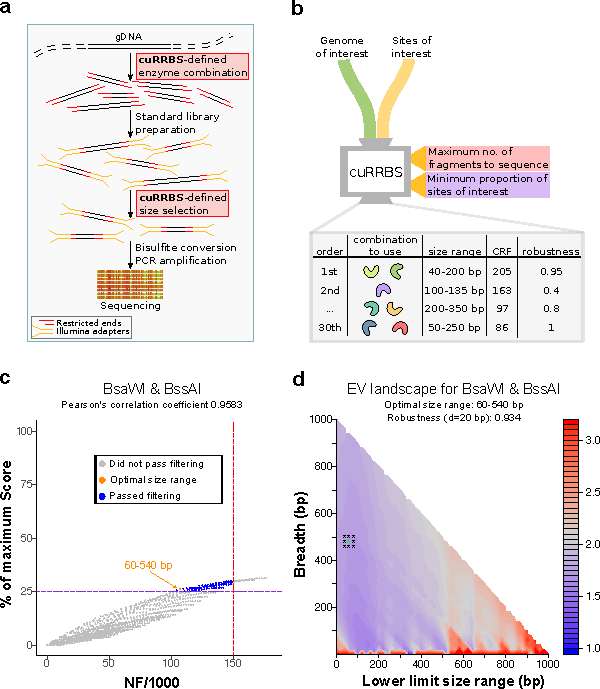
\includegraphics[width=0.9\textwidth]{C4_Fig3}
	%\vspace*{3mm}
	\caption[cuRRBS overview]{cuRRBS overview. \textbf{a.} Outline of an RRBS protocol. Highlighted are the two steps that would be modified according to the output produced by cuRRBS (i.e. the restriction enzymes used for the genomic digestion and the size selection). Legend is displayed on the bottom left. \textbf{b.} Schematic of cuRRBS. Highlighted are the two main inputs required for the software and the two \textit{thresholds} that the user has to define (red and purple tags). The default output for cuRRBS is a table containing the top hits (restriction enzyme combination and size range) along with additional information that might be useful to the user (such as \textit{Cost Reduction Factor} and \textit{robustness}). \textbf{c.} Scatterplot showing the trade-off between the number of fragments (\textit{NF}) and the \textit{Score} for the best enzyme combination (BsaWI \& BssAI) that targets the CpGs present in the human placental-specific imprinted regions \citep{Hanna2016}. \textit{NF} is divided by 1000 for visualization purposes. Each point represents a different \textit{size range}. Shown in dark blue and grey are the size ranges that would and would not pass filtering respectively. Shown in orange is the optimal size range in the filtered search space. The dotted lines depict the \textit{thresholds} that need to be specified by the user (red: maximum \textit{NF}; purple: minimum percentage of the maximum \textit{Score}). In this mock example we specified an \textit{NF threshold} of 150000 fragments and a \textit{Score threshold} of $25\%$ of the maximum \textit{Score}. Legend is displayed below the plot title. \textbf{d.} Contour plot that depicts how the \textit{robustness} (\textit{R}) variable is calculated for the optimal enzyme combination (BsaWI \& BssAI; size range: 60-540 bp) that targets the CpGs present in the human placental-specific imprinted regions \citep{Hanna2016}. \textit{Enrichment values} (\textit{EVs}) are calculated for all possible size ranges in order to create an \textit{EV} `landscape'. In this landscape, cuRRBS finds the size range with the lowest \textit{EV} that still satisfies the \textit{thresholds} (asterisk in green). Afterwards, cuRRBS samples \textit{EV}s around the optimum (asterisks in black). The points that are sampled depend on the experimental error (in this case, $\delta = 20$ bp). A high \textit{robustness} value means that the sampled \textit{EV}s do not change a lot when compared to the optimum, which implies that cuRRBS prediction will not be greatly affected by experimental errors during the size selection step.}
	\label{fig:c4_fig3}
\end{figure}


\section{Running cuRRBS in different biological systems}

\smallskip

cuRRBS provides a way to effectively interrogate DNA methylation in any biological system (including the CpG sites that constitute different epigenetic clocks) for which the reference genome is available. Besides reducing the cost for organisms currently under intensive study (e.g. human, mouse), cuRRBS opens the door to the cost-effective study of DNA methylation in species with large genomes or where DNA methylation in non-CpG contexts is common, such as plants \citep{Stroud2013}, which currently lack an MspI-based RRBS protocol, owing to the enzyme’s CHG methylation sensitivity \citep{Sun2014}.

\bigskip

We decided to test the ability of cuRRBS to enrich for genomic sites that have important functional roles in different systems. Some of the systems that we tested \textit{in silico} include genomic regions whose methylation status is important during cellular reprogramming \citep{Milagre2017}, Horvath's epigenetic clock \citep{Horvath2013}, transcription factor binding sites that are affected by DNA methylation \citep{Maurano2015,Domcke2015}, imprinted loci \citep{Hanna2016}, CpGs found in the exon-intron boundaries \citep{LevMaor2015} and CHG sites that are differentially methylated between different arabidopsis accessions \citep{Kawakatsu2016} (Fig.~\ref{fig:sc4_fig5}). For these \textit{in silico} systems we chose to run the software with the threshold set to $25\%$ of the maximum \textit{Score}.

\bigskip

In all cases, \textbf{cuRRBS is able to dramatically reduce the cost associated with the sequencing} by several orders of magnitude compared to WGBS, which is assessed using the \textit{Cost Reduction Factor} ($CRF$) (Fig.~\ref{fig:c4_fig4}). In addition, for cases where a comparison to MspI-based RRBS could be made, cuRRBS is able to improve the \textit{CRF}, again, by orders of magnitude. As an example, for the placental-specific imprints, the sequencing costs are reduced by approximately 400-fold when compared to WGBS and by 12.5-fold when compared to the traditional MspI-based RRBS.

\bigskip

Furthermore, we have also observed that many of the top hits reported by cuRRBS are digestions of two restriction enzymes (Fig.~\ref{fig:sc4_fig5}), highlighting the combinatorial power of restriction enzymes to produce optimal reduced representations of the genome \citep{Bystrykh2013}. Excitingly, we are able to show that using cuRRBS it is possible to assay a far larger number of target sites, in a far simpler experimental design than would normally be achieved using amplicon-based bisulfite sequencing.


\begin{figure}[htbp!] 
	\centering    
	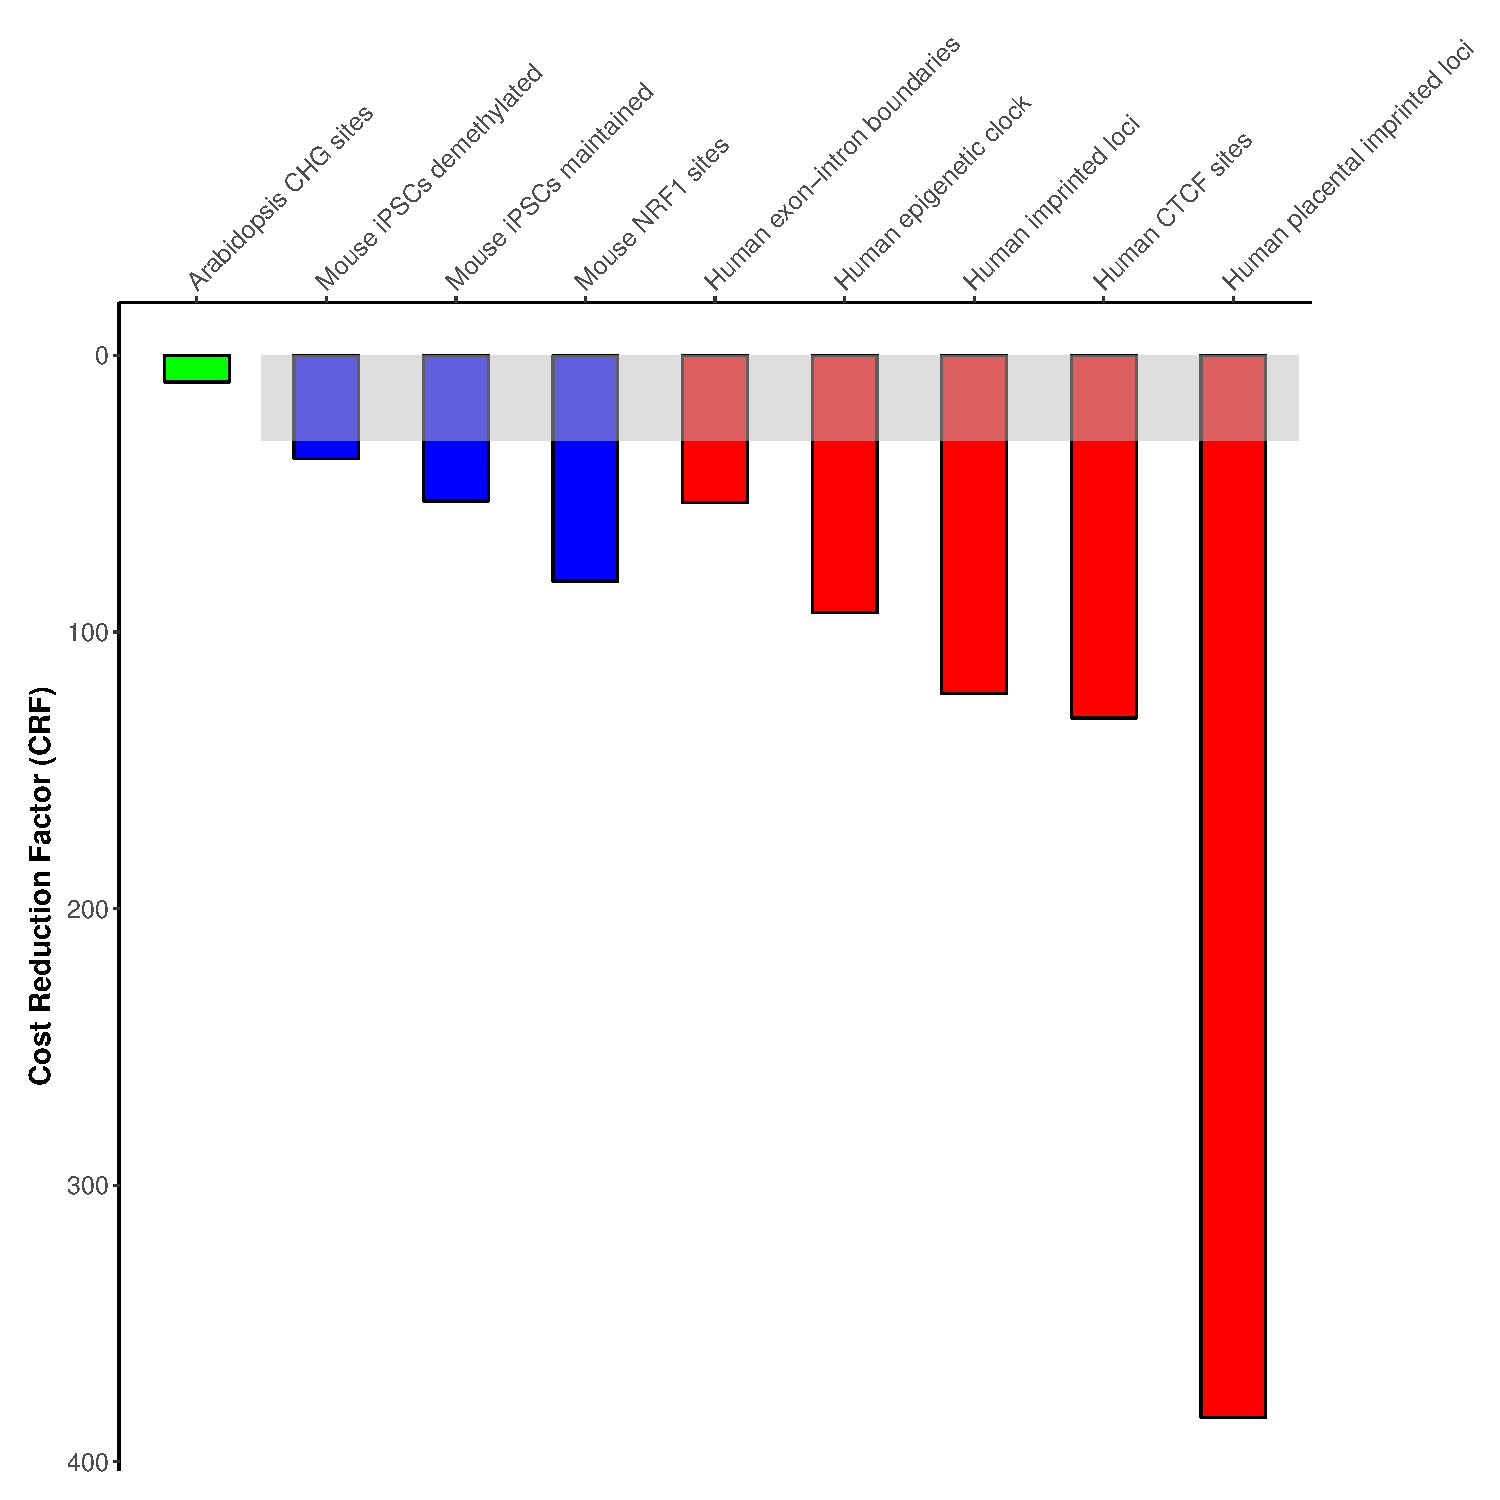
\includegraphics[width=0.5\textwidth]{C4_Fig4}
	%\vspace*{3mm}
	\caption[Running cuRRBS in different biological systems]{Running cuRRBS in different biological systems. Barplot showing the values for the \textit{Cost Reduction Factor} (\textit{CRF}) in the different biological systems that were tested (see Fig.~\ref{fig:sc4_fig5}) \citep{Horvath2013,Hanna2016,Milagre2017,Kawakatsu2016,Maurano2015,LevMaor2015,Domcke2015}. The colours in the bars represent the different species interrogated (green: \textit{Arabidopsis thaliana}, blue: \textit{Mus musculus}, red: \textit{Homo sapiens}). The \textit{CRF} for the traditional RRBS protocol (MspI in the human genome, using a bead size selection step of 20-800 bp, $CRF = 30.65$) is displayed as a grey area, which is not compared with the \textit{A. thaliana} system (since MspI is sensitive to CHG methylation).}
	\label{fig:c4_fig4}
\end{figure}


\smallskip

\section{Experimental validation of cuRRBS} \label{s:4.5}

\smallskip

To assess in an unbiased manner how well predictions from cuRRBS perform in an experimental setting, we employed two independent non-canonical RRBS datasets: one generated from a single enzyme (XmaI) and the other from a combination of two restriction enzymes (MspI and Taq$^\alpha$I) \citep{Tanas2017,Lim2016}. By evaluating the predictive power of cuRRBS in these two datasets, we were able to observe cuRRBS' performance in both single and double enzyme contexts and across different genomes.

\bigskip

To test the accuracy of cuRRBS predictions \textbf{in the context of a single enzyme digestion}, we utilised the non-canonical RRBS dataset generated from human DNA using the restriction enzyme XmaI \citep{Tanas2017}. This dataset was previously used to show that XmaI could enrich for CpG islands (\acrshort{CGI}s), while reducing the overall sequencing cost relative to MspI, making the protocol more cost-effective. To validate cuRRBS using this system, we therefore chose to enrich for all CpG sites that overlapped with a CGI (CGI-CpGs) in the human genome using a predetermined theoretical size range equivalent to the `reproducible library fragment lengths' reported in \citep{Tanas2017} (i.e. 90-185 bp). cuRRBS predicted with high accuracy the CpG sites that were observed in the experimental XmaI-RRBS dataset (Fig.~\ref{fig:c4_fig5}a). In particular, only a small proportion of the total number of CGI-CpGs should be theoretically sequenced (102253 out of 2164614 i.e. 4.72\%), and this was indeed the case (Fig.~\ref{fig:c4_fig5}a). Furthermore, upon filtering out sites with low depth of coverage, which commonly represent noise in RRBS datasets, the sensitivity increased up to approximately 80\%. Importantly, the specificity remained constant at almost 100\% independent of the threshold set for depth of coverage (Fig.~\ref{fig:c4_fig5}b). Thus, cuRRBS produces a prediction that is relatively conservative, as highlighted by the low numbers of false positives (Fig.~\ref{fig:c4_fig5}a), at the expense of a small decrease in sensitivity.

\bigskip

Interestingly, the original theoretical size range that the study was aiming for (110-200 bp) was slightly different to the one achieved in the actual experiments (90-185 bp) \citep{Tanas2017}. We ran cuRRBS using the original size range target and obtained slightly worse results for the sensitivity but not the specificity of the prediction (Fig.~\ref{fig:sc4_fig6}). This demonstrates that the correct execution of the size selection step during the experimental protocol is key for obtaining the sites predicted by cuRRBS and highlights the importance of the \textit{robustness} variable as part of the cuRRBS output in order to judge the consequences of these experimental errors.

\begin{figure}[htbp!] 
	\centering    
	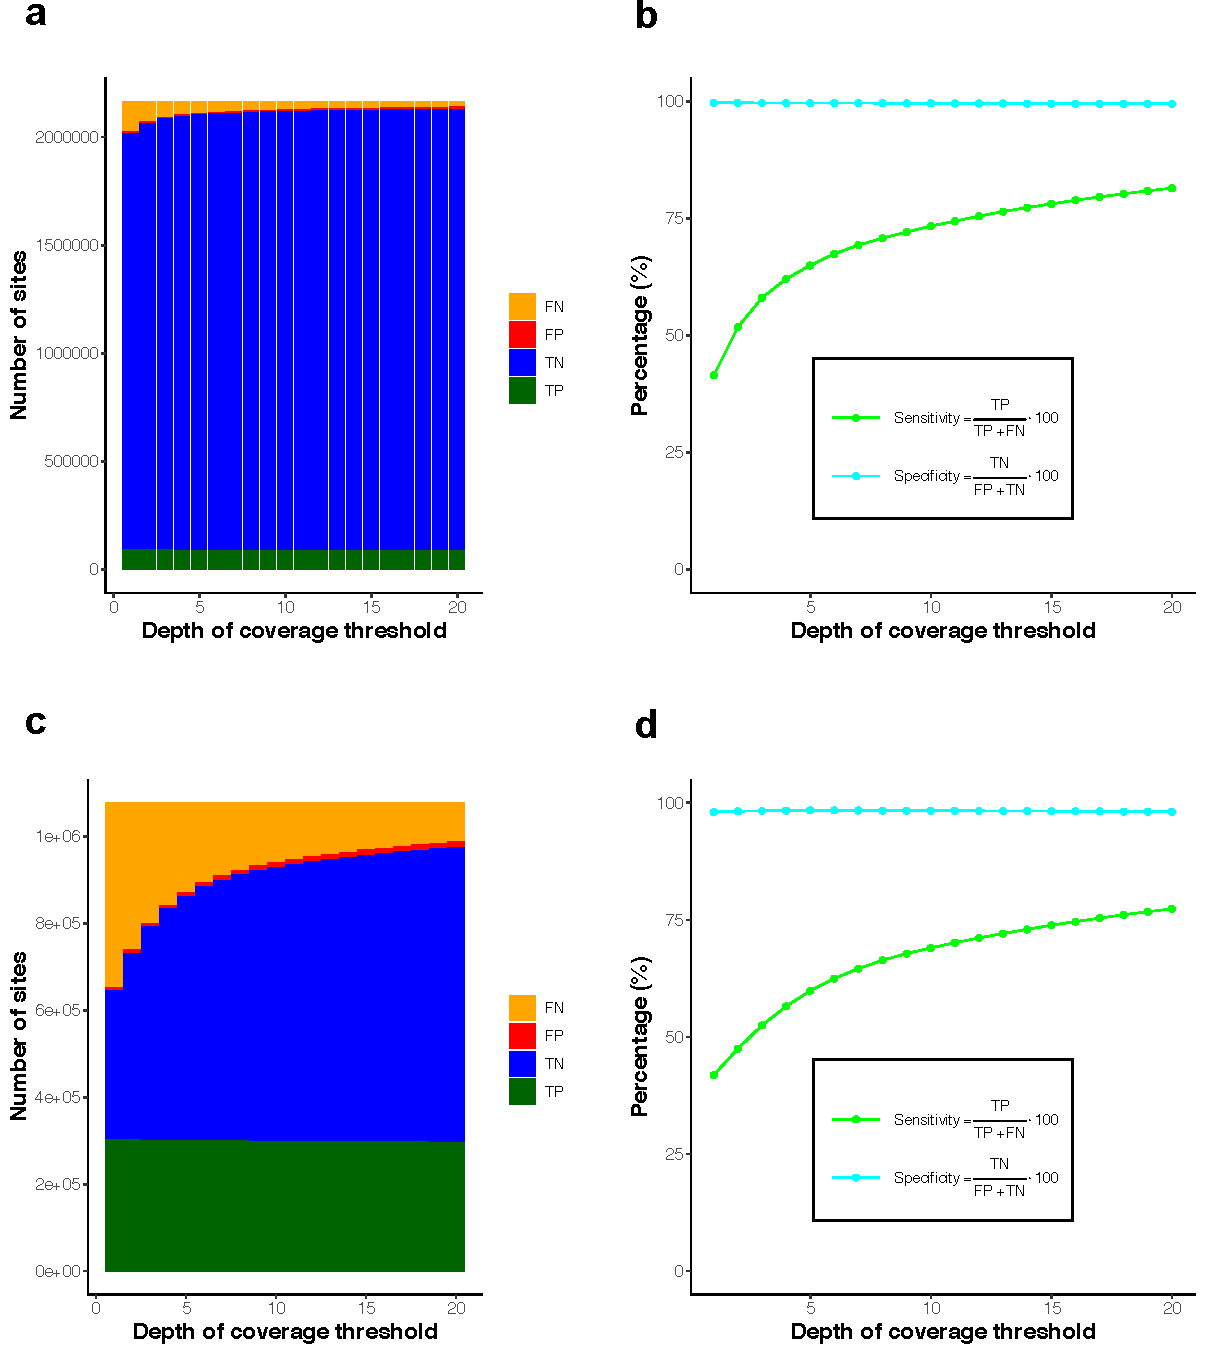
\includegraphics[width=1\textwidth]{C4_Fig5}
	\vspace*{2mm}
	\caption[Experimental validation of cuRRBS]{Experimental validation of cuRRBS. \textbf{a.} Barplots showing the number of true positives (\acrshort{TP}, in green), true negatives (\acrshort{TN}, in blue), false positives (\acrshort{FP}, in red) and false negatives (\acrshort{FN}, in orange) when comparing cuRRBS theoretical prediction with the actual XmaI-RRBS experimental data \citep{Tanas2017} (see section~\ref{s:4.7} for more details). The number of sites in each category is calculated for different thresholds in the depth of coverage (number of reads covering a CpG site as reported by Bismark). cuRRBS prediction for the CpG sites in human CpG islands was obtained enforcing a theoretical size range of 90-185 bp and running the software for XmaI with all the default parameters (with a \textit{read length} of 200 bp). Legend is displayed on the right hand side. \textbf{b.} Plot showing values of cuRRBS sensitivity (in light green) and specificity (in cyan) as a function of the depth of coverage threshold employed to filter the experimental data \citep{Tanas2017}. The number of true positives (TP), true negatives (TN), false positives (FP) and false negatives (FN) are the same as in a. Legend is displayed below the plot curves. \textbf{c.} Same as in a. but for the MspI\&Taq$^\alpha$I-RRBS experimental data \citep{Lim2016}. cuRRBS prediction for the CpG sites in mouse CpG islands was obtained enforcing a theoretical size range of 80-160 bp and running the software for MspI\&Taq$^\alpha$I with all the default parameters (with a \textit{read length} of 75 bp). \textbf{d.} Same as in b. but for the MspI\&Taq$^\alpha$I-RRBS experimental data \citep{Lim2016}.}
	\label{fig:c4_fig5}
\end{figure}

\bigskip

To test the accuracy of cuRRBS predictions \textbf{in the context of a double enzyme digestion}, we utilised the non-canonical RRBS dataset generated from mouse DNA using the restriction enzymes MspI and Taq$^\alpha$I \citep{Lim2016}. To compare the accuracy of cuRRBS prediction in this double enzyme system to that of the XmaI-RRBS system, we again ran cuRRBS for CGI-CpGs, this time in the mouse genome with a theoretical size range of 80-160 bp \citep{Lim2016}. cuRRBS predicted with high accuracy the CpG sites that were observed in this double enzyme experiment (Fig.~\ref{fig:c4_fig5}c). In addition, the results for sensitivity and specificity were very similar to the ones reported for the XmaI-RRBS dataset (Fig.~\ref{fig:c4_fig5}d). Therefore, we conclude that cuRRBS produces robust predictions for the sites of interest that will be sequenced in RRBS protocols both for single and double enzyme combinations independent of the genome under study.

\bigskip

Lastly, the number of fragments that were theoretically recoverable in each of our experimental systems ranged from $NF = 12780$ (for XmaI) to $NF = 331058$ (for MspI and Taq$^\alpha$I). This represents approximately a 30-fold difference in the number of recoverable fragments and demonstrates that cuRRBS predictions, even for low $NF$ values, are experimentally feasible. Importantly, in the nine theoretical examples that we report (Fig.~\ref{fig:sc4_fig5}), the number of fragments required by each cuRRBS protocol ranges from 107248 to 974050. Thus, the number of fragments required to achieve the stated $CRF$ comfortably exceeds the minimum experimentally validated $NF$ value (>8-fold). 

\smallskip

\section{Conclusions and future directions}

\smallskip

cuRRBS provides a new framework that allows the user to optimise RRBS for the biological system of interest by using novel combinations of restriction enzymes. Therefore, cuRRBS makes the study of DNA methylation more affordable across all species for which genomic sequences are available. Furthermore, it can open the door to the design of future studies in a clinical context \citep{Lee2014}, which require cost-effective and robust protocols.

\bigskip

Currently, cuRRBS only considers combinations of up to two restriction enzymes. However, in the future, it would be possible to adapt the software to explore combinations that contain higher numbers of enzymes, which could theoretically allow targeting the sites of interest even more efficiently \citep{Bystrykh2013}. Moreover, there are several methods that are able to impute DNA methylation levels in sites that are not covered experimentally \citep{Zhang2015,Angermueller2017}. These methods could expand the set of sites of interest that are finally measured by making use of the additional DNA methylation information that is retrieved in a cuRRBS experiment. 

\bigskip

Finally, the potential of restriction enzymes to target different genomic coordinates is not limited to DNA methylation. As such, it would be conceivable for cuRRBS to be adapted to enrich for SNPs of interest \citep{Davey2011,Davey2011a} or to optimise chromosome conformation capture techniques \citep{Naumova2012,Dekker2013}. By reducing the cost associated with sequencing, we believe that cuRRBS will help to democratise high-throughput genomic studies. 

\smallskip

\section{Additional methods} \label{s:4.7}

\subsection*{Restriction enzymes annotation}

All the information regarding the commercially-available restriction enzymes that are used by cuRRBS was extracted from REBASE \citep{Roberts2005,Roberts2015}. Restriction enzymes were grouped in isoschizomer families (i.e. enzymes that recognise the same sequence and generate identical fragment length distributions) and each enzyme was manually annotated for different types of methylation-sensitivity (CpG, CHG, \acrshort{CHH}). Only isoschizomer families that contained at least one methylation-insensitive enzyme were considered for the examples described here.

\subsection*{Genome assemblies and genomic annotation}

All the analyses presented here were performed in the following genome assemblies: \textit{Homo sapiens} (hg38), \textit{Mus musculus} (mm10) and \textit{Arabidopsis thaliana} (TAIR10). Scaffolds not assembled into the main chromosomes were discarded. Genomic annotation for the human genome (hg38) was obtained from GENCODE (v25, basic gene annotation) \citep{Harrow2012}, with the exception of CpG islands (CGIs), which were extracted from the UCSC Genome Browser \citep{Bock2007}. GC content and CpG content were calculated, around each restriction enzyme cleavage site, taking windows of  ± 25 bp and ± 500 bp respectively. For each enzyme, the mean of all cleavage sites was calculated to obtain the mean GC content and the mean CpG content. Intragenic regions were defined as those regions within ± 2.5 \acrshort{kb} of a protein-coding gene, whilst the rest of the genome was considered to be intergenic. CpG shores were defined as regions 0 to 2 kb away from CGIs in both directions and CpG shelves as regions 2 to 4 kb away from CGIs in both directions \citep{Zhang2015}. Promoters were defined as encompassing a 3 kb region (2.5 kb upstream and 0.5 kb downstream of the  \acrshort{TSS}) relative to the TSS of all protein-coding transcripts in GENCODE, similar to the strategy used in \citet{Taher2013}. Genomic annotation for the CGIs in the mouse genome (mm10) was also obtained from the UCSC Genome Browser \citep{Bock2007}. All annotations were handled using the \textit{pybedtools} library \citep{Quinlan2011,Quinlan2010}.

\subsection*{Performing \textit{in silico} digestions of a given genome}

We used the \textit{Restriction} package from Biopython v1.68 to digest the different genomes with the appropriate restriction enzymes \textit{in silico} \citep{Cock2009}. Only the first member of a given isoschizomer family (which contained at least one methylation-insensitive enzyme) was processed to avoid redundant computations. The output of the \textit{in silico} digestions was stored (pre-computed files) and subsequently read by cuRRBS when needed to reduce the computational time (see `cuRRBS heuristics and computational efficiency'). When assessing enzyme combinations, the information from the appropriate individual pre-computed files (i.e. the genomic coordinates where the enzyme theoretically cuts) were combined by the software to compute all the necessary variables.

\subsection*{cuRRBS' enzyme flexibility}

To ensure the user has full control over the enzymes that cuRRBS will use to derive the desired enrichments, one of the inputs given to cuRRBS is an enzyme annotation file. This file contains the desired isoschizomer families that the user wishes to be tested by cuRRBS. In my \href{https://github.com/demh/cuRRBS/tree/master/utils}{GitHub repository} we have already defined enzyme annotation files for enzymes that are methylation-insensitive in a CG context and in CG, CHG and CHH contexts \citep{Martin-Herranz2017}. However, it is also possible for the user to define a personalised set of enzymes by providing a self-generated annotation file. This can be useful, for instance, to reduce the chance of any star activity in the reported cuRRBS protocols.

\bigskip

In addition, the output file from cuRRBS contains, by default, 30 cuRRBS protocols that would enrich for the user's sites of interest. Therefore, the user can determine which enzyme combination and size range would be the simplest and most appropriate for the given application. This provides the user with the opportunity to consider experimental factors that may complicate the protocol, such as buffer compatibility and whether consecutive digestions would be required.

\subsection*{Flexible user-defined cuRRBS parameters}

cuRRBS contains a number of user-defined parameters to ensure the greatest possible flexibility and ease of use. A table of these parameters is provided to highlight the versatility that the user has and why such versatility is useful (Table~\ref{table:c4_table1}).

\begin{table}
	%\centering
	\small
	\begin{tabular}{ p{5cm} p{6.5cm} p{1cm} p{1.5cm} }
		\toprule
		\textbf{cuRRBS parameter (abbrev.)} & \textbf{Significance} & \textbf{Default} & \textbf{Range} \\ 
		\midrule
		Enzymes to check (-e) &  Defines the enzymes (isoschizomer families) that cuRRBS will look at & -  & -  \\
		
		Annotation for the sites of interest (-a) & Allows identification and weighting of the sites of interest & - & - \\
		
		Read length (-r) & Defines the positions in the theoretical fragments that can be `seen' after sequencing & - & 30-300 \\
		
		Adapters size (-s) & Ensures correct experimental size selection & - & - \\
		
		C\_Score constant (-c) & Sets the minimum acceptable $Score$ & - & 0-1  \\
		
		Genome size (-g) & Needed to calculate the $CRF$ & - & - \\
		
		C\_NF/1000 constant (-k) & Sets the minimum acceptable $CRF$ & 0.2 & 0-1 \\
		
		Experimental error (-d) & Sets the assumed experimental error ($\delta$) & 20 & 5-500  \\
		
		Size range breadth (-b) & Constrains the breadth of the size range & 980 & - \\
		
		Output size (-t) & Defines the number of cuRRBS protocols the user can compare & 30 & - \\
		
		Site IDs (-i) & Enables the identification of the recovered sites of interest & No & - \\
		\bottomrule
	\end{tabular}
	\vspace*{3mm}
	\caption[Flexible user-defined cuRRBS parameters]{Flexible user-defined cuRRBS parameters. This table details the flexible user-defined parameters that cuRRBS will accept as arguments. The cuRRBS parameter full name and command line abbreviation (in brackets) are provided alongside a simplified description of the significance of these arguments to the user. Where applicable, the defaults and ranges of these arguments are also detailed.}
	\label{table:c4_table1}
\end{table}


\subsection*{cuRRBS heuristics and computational efficiency}

cuRRBS employs several strategies to reduce the computational time needed in each run:

\begin{itemize}
	
	\item Restriction enzymes are grouped in isoschizomer families. Since isoschizomers generate the same genomic digestions, only one member of each family needs to be processed. 
	
	\item \textit{In silico} digestions are read from pre-computed files. Digesting the genomes would be a limiting factor in the cuRRBS pipeline. The user can download the pre-computed files \citep{Martin-Herranz2017} and the information that they contain is read every time that an enzyme needs to be assessed.
	
	\item The number of size ranges that are sampled is minimised. Since the experimental size selection step is generally imperfect, size ranges are sampled with a sliding window whose `resolution' is equivalent to the experimental error specified by the user. 
	
	\item Parallelization. cuRRBS can use several cores to decrease the \acrshort{CPU} time.

\end{itemize}

Moreover, we have observed that, in many enzyme combinations, one of the enzymes is providing most of the enrichment for the sites of interest, while the second one complements the targeting. Therefore, it would be possible to implement a `heuristic' mode, where only those enzymes that perform well individually are used as `seeds' to construct combinations (as opposed to the current implementation, where all the enzyme combinations are checked exhaustively). This could further reduce the computational time, especially if combinations of more than two enzymes were being evaluated. 

\bigskip

The CPU time required by cuRRBS depends on several parameters, including the number of enzymes checked, the experimental error, the number of sites of interest or the genome size (Fig.~\ref{fig:sc4_fig7}). The RAM used will be approximately equal to the size of the pre-computed files that are read by the software. A standard cuRRBS run (e.g. for a few thousand sites of interest in the human genome, checking 128 CpG methylation-insensitive isoschizomer families) \textbf{takes around 0.5-1 hours and uses around 4 \acrshort{GB} \acrshort{RAM}}, which allows the user to easily run it on a dual-core laptop or desktop computer. 


\subsection*{Obtaining the sites of interest for different biological systems}

We have tested \textit{in silico} the ability of cuRRBS to enrich for the sites of interest in a selection of different biological systems where DNA methylation has an important functional role. In some of these systems, described below, previous analysis was performed in order to obtain the genomic coordinates for the sites:

\begin{itemize}

	\item Exon-intron boundaries in human. Exons and introns were obtained from protein-coding genes using GENCODE annotation data. Those CpG sites that were found within ± 5 bp of a canonical splice site (5'-GT, 3'-AG) were selected.
	
	\item Epigenetic clock in human. These sites were obtained from the Horvath epigenetic clock \citep{Horvath2013} and were lifted over to hg38 \citep{Kuhn2012} before running cuRRBS.
	
	\item Canonical and placental imprints in human. These loci were obtained from \citet{Hanna2016}. The sites were lifted over to hg38 \citep{Kuhn2012} and the CpG sites were then extracted for the analysis. 
	
	\item \acrshort{CTCF} binding sites in human. We obtained the CpG sites that overlap with \textit{in vivo} CTCF binding sites. Peaks from sites that seem to be affected by methylation (upregulated, reactivated) were kindly provided by Dr. M. T. Maurano \citep{Maurano2015}. We scanned the peaks for high-scoring motifs according to the CTCF JASPAR model \citep{Zhang2015a}. Finally, we extracted those CpGs that were found in positions 5 and 15 of the motif, whose methylation status is supposed to influence the binding of the transcription factor \citep{Maurano2015}. 
	
	\item Induced pluripotent stem cells (\acrshort{iPSCs}) demethylated and maintained sites in mouse. These were obtained by comparing mouse embryonic fibroblasts (\acrshort{MEFs}) to iPSCs as described previously \citep{Milagre2017}, with an additional filter for magnitude of methylation change (>50$\%$ methylation change).
	
	\item \acrshort{NRF1} binding sites in mouse. We obtained the CpG sites that overlap with \textit{in vivo} NRF1 binding sites in mouse. \acrshort{ChIP-seq} data was processed as described in the original publication \citep{Domcke2015}, where peaks were called using Peakzilla \citep{Bardet2013}. We took as our final set of peaks the overlap between the two \acrshort{TKO} replicates. Next, we scanned the peaks for high-scoring motifs according to the NRF1 JASPAR model \citep{Zhang2015a}. Finally, we extracted those CpGs that were found in positions 2 and 8 of the motif, whose methylation status is supposed to influence the binding of the transcription factor \citep{Zhang2015a}.
	
	\item CHG sites in \textit{Arabidopsis thaliana}. Non-CpG DMRs arising from the epigenomic diversity between \textit{Arabidopsis thaliana} accessions were obtained from \citet{Kawakatsu2016}. The coordinates for C sites in non-CpG context were extracted.
	
	
\end{itemize}

In all the cases the sites were equally weighted ($w_i = 1$), with the exception of the human epigenetic clock system, where the sites were assigned the absolute value of the weights in the linear model \citep{Horvath2013}. All the site annotation files can be found in my \href{https://github.com/demh/cuRRBS/tree/master/examples}{GitHub repository} \citep{Martin-Herranz2017}


\subsection*{Running cuRRBS for the different biological systems}

cuRRBS was run in the different systems described above using the default parameters ($k = 0.2$, $d = 20$, $b = 980$, $t = 30$), for a \textit{read length} (\textit{r}) of 75 bp and a \textit{Score threshold} (\textit{c}) of 0.25. In the mouse and human examples we considered 128 isoschizomer families that contained enzymes that were not sensitive to CpG methylation. In the case of \textit{Arabidopsis thaliana} we used 28 isoschizomer families that contained enzymes that were not sensitive to 5mC in any context (\acrshort{CG}, CHG, CHH).


\subsection*{Mapping of RRBS samples}

XmaI-RRBS data generated on the Ion Torrent platform \citep{Tanas2017} and MspI\&Taq$^\alpha$I -RRBS data generated on the Illumina HiSeq platform \citep{Lim2016} were quality trimmed using Trim Galore (www.bioinformatics.babraham.ac.uk/projects/trim\_galore/) and had base pairs removed from the 3' end to avoid including filled-in nucleotides with artificial methylation states (the filled-in XmaI, MspI and Taq$^\alpha$I cut sites include the nucleotide sequence CCGG, CG and CG respectively). The data was then mapped to the human genome (for XmaI data, parameters: --non\_directional) or the mouse genome (for MspI\&Taq$^\alpha$I  data, parameters: --directional) using Bismark (0.18.0) \citep{Krueger2011}. In each of the two cases data from different experiments or replicates was merged into the same FASTQ file prior to quality trimming.

\subsection*{Estimating cuRRBS' sensitivity and specificity }

We assessed the performance of cuRRBS predictions in two independent experimental datasets \citep{Tanas2017,Lim2016} (see section~\ref{s:4.5}). We ran cuRRBS fixing the theoretical size ranges tested to the ones reported in the publications \citep{Tanas2017,Lim2016} and we used as our sites of interest the CpGs that overlapped with CpG islands (CGI-CpGs) in the human \citep{Tanas2017} and the mouse genomes \citep{Lim2016} respectively. From the cuRRBS output files we recovered the IDs of the sites that should be theoretically sequenced. Moreover, using the experimental RRBS data \citep{Tanas2017,Lim2016}, we could obtain the IDs of the sites that were actually sequenced (filtered by a given depth of coverage threshold). Afterwards, we calculated the following variables for each one of the datasets:

\begin{itemize}
	
	\item True positives (TP): number of CGI-CpGs that cuRRBS predicted to be sequenced and were indeed found in the RRBS data.
	
	\item True negatives (TN): number of CGI-CpGs that cuRRBS predicted to be absent and were not found in the RRBS data.
	
	\item False positives (FP): number of CGI-CpGs that cuRRBS predicted to be sequenced but were not found in the RRBS data.
	
	\item False negatives (FN): number of CGI-CpGs that cuRRBS predicted to be absent but were found in the RRBS data.
	
\end{itemize}

Finally, we estimated the sensitivity and specificity, for a given dataset, as follows:

\begin{align}
Sensitivity = \frac{TP}{TP+FN} \cdot 100
\end{align}

\begin{align}
Specificity = \frac{TN}{FP+TN} \cdot 100
\end{align}

\subsection*{Software availability}

cuRRBS and its documentation are freely distributed under GNU General Public License v3.0 and can be accessed in my \href{https://github.com/demh/cuRRBS/}{GitHub repository} \citep{Martin-Herranz2017}.
%!TEX root = ../thesis.tex
%*******************************************************************************
%****************************** Fifth Chapter *********************************
%*******************************************************************************

\chapter{Final remarks} \label{c:5}

\ifpdf
	\graphicspath{{Chapter5/Figs/pdf/}}
\else
	\graphicspath{{Chapter5/Figs/svg/}}
\fi

\epigraph{`Caminante, son tus huellas \\ el camino, y nada más; \\ caminante, no hay camino: \\ se hace camino al andar.}{Antonio Machado, 1912 \cite{Machado}}

\bigskip

The purpose of this thesis was to advance our understanding of the epigenetic ageing clock in humans. I now review the main conclusions from this work and propose future directions that could be of interest.


\section{Statistical aspects}

\bigskip

In Chapter~\ref{c:2}, I have assessed different statistical methods that allowed me to \textbf{characterise the epigenetic landscape during human physiological ageing}. To date, DNA methylation data from blood, generated in the Illumina 450K methylation array platform, is the most abundant epigenetic data type available to study human ageing. I built a dataset of this data type for healthy individuals, pre-processed it and benchmarked different methods to correct for blood cell composition changes. I reproduce previous findings showing that a great proportion of the epigenome is affected by the ageing process (in my case around 30\%, using a conservative threshold to correct for multiple testing). This highlights that the epigenetic ageing clock is a genome-wide phenomena that extends way beyond the cytosines included in most epigenetic clock models. Furthermore, the small effect sizes suggest that most age-related DNA methylation changes occur only in a small proportion of cells (DNA molecules) in the tissue (around 4\% on average for the entire human lifespan). Finally, I tested the behaviour of different epigenetic clocks (Horvath, Hannum, epiTOC) and developed a strategy to correct for potential batch effects in this context.

\bigskip

Current epigenetic clocks use a linear modelling framework. Nevertheless, many changes in methylation values during ageing are non-linear (for example during organismal growth). Horvath's clock corrects for this by transforming chronological age, but it would be interesting to try to model the changes of individual CpG sites before including them as part of the training. This could also help to identify modules of CpG sites that behave in the same way during ageing and allow deconvoluting the different processes that shape the epigenetic landscape and may be operative at different life stages. Additional \textbf{improvements in epigenetic clocks} will likely include integrating longitudinal information (which could help to identify different ageing trajectories) \cite{Jensen2014} and separating the contributions of mutations and epimutations to the methylation signal. Furthermore, it would be interesting to try to map the shapes of the DNA methylation changes to the changes in mortality rate at a human population level, therefore creating a link between molecular changes and epidemiological observations. This could be further validated in species with extremely different profiles of mortality rate (e.g. naked mole rat).

\bigskip

Current multi-tissue epigenetic clocks have been trained on all tissues available. Nevertheless, it is reasonable to assume that the strategies to maintain stable DNA methylation landscapes over time would significantly differ between highly proliferative tissues (such as blood) from those where cell division is a rare event (such as brain). Thus, building different epigenetic clocks for these two categories of tissues and analysing their genome-wide changes in DNA methylation over time could improve the accuracy of the models and provide \textbf{further insights into the role of cell division on the epigenetic ageing clock}.

\bigskip

There are methods that allow imputing DNA methylation patterns based on different genomic features for a `static' epigenome, both at the bulk \cite{Zhang2015} and single-cell levels \cite{Angermueller2017,Kapourani2019}. Given that the regions that change their DNA methylation during ageing seem to share the genomic context, it would be interesting to design an \textbf{imputation algorithm for a `dynamic' epigenome} (e.g. given an epigenome at time $t$, predict what that epigenome would look like at time $t + \Delta t$). This could also give us additional insights into how much the ageing-related changes are hard-coded in the genome and how much the environment and lifestyle contribute to modify it. Moreover, some of these predictions could be tested by introducing exogenous pieces of DNA in ageing mice.

\bigskip

Developmental disorders are useful biological systems to study the effects of altered functions in specific parts of the epigenetic machinery. As such, the analysis presented in Chapter~\ref{c:3} could be further expanded into a statistical framework that allows quantifying how much certain epigenetic functions contribute to the methylation status of specific regions. In other words, the definition of \textbf{epimutational signatures} (e.g. epimutational signature 1 is the consequence of reduced H3K4 methylation in enhancers) that would allow to deconvolute the epigenetic processes behind a specific DNA methylation pattern (e.g. the one caused by ageing or smoking exposure).

\smallskip

\section{Biological aspects}

\smallskip

The goal of Chapter~\ref{c:3} was to study \textbf{how different parts of the epigenetic machinery affect the rate of the epigenetic ageing clock}, thus providing the first identified components of the hypothetical \textit{epigenetic maintenance system} \cite{Horvath2013}. For that purpose, I studied the epigenetic age acceleration observed in patients with developmental disorders, many of which harbour mutations in proteins of the aforementioned epigenetic machinery.

\bigskip

This analysis revealed that \textbf{mutations in NSD1, an H3K36 methyltransferase, dramatically accelerate epigenetic ageing}. The effect sizes observed (on average > 7 years) are bigger than many of the conditions reported to accelerate the epigenetic ageing clock \cite{Horvath2018}. Importantly, the genomic context where these changes happen is partially shared with the ageing process. Regions marked by H3K27me3, deposited by Polycomb Repressing Complex 2 (\acrshort{PRC2}), were highly enriched for these changes both in ageing and Sotos, consistent with previous reports. Interestingly, global DNA hypomethylation (a characteristic of Sotos patients) causes a redistribution of \acrshort{PRC2} and H3K27me3 from their normal targets (many of them developmental genes marked with bivalent chromatin) to other genomic regions, which leads to the aberrant expression of some of these genes \cite{Reddington2013}. Importantly, there is a mechanistic link between PRC2 recruitment and H3K36me3 via the Tudor domains of some polycomb-like proteins \cite{Cai2013,Li2017}. As such, it would be expected that perturbations in the H3K36 methylation landscape would affect PRC2 activity. Furthermore, methylation of CpG sites in normally unmethylated CpG islands could also lead to a loss of PRC2 binding \cite{Li2017}. This could be happening in bivalent regions / DNA methylation valleys (\acrshort{DMV}s) during ageing and affect the differentiation process of progenitor stem cells in adult tissues. Indeed, this seems to be the case for aged haematopoietic stem cells \cite{Sun2014x,Beerman2013}, but whether this applies to other tissues still needs to be elucidated. Importantly, DNA methylation changes affecting progenitor stem cells could be propagated in the tissue, therefore contributing substantially to the signal captured by epigenetic clocks. 

\bigskip

Hence, during ageing, there could be a  \textbf{redistribution of \acrshort{PRC2} from bivalent regions / \acrshort{DMV}s to other regions that have become hypomethylated, at the same time that \textit{de novo} DNMT3A/B get relocated in the opposite direction} (as shown in Fig.~\ref{fig:c3_fig8}), leading to a deregulation in the expression of developmental genes. This model expands and is overall compatible with the one proposed by Zheng, Widschwendter and Teschendorff to explain the increase in cancer risk with age \cite{Zheng2016}. While this could be induced by the rewiring of the H3K36 methylation landscape, direct evidence needs to be provided to ascertain that this is indeed the case during human physiological ageing. As such, it would be interesting to profile H3K36me3 during ageing in different tissues. Furthermore, differential expression of genes coding for the H3K36 methylation machinery (both methyltransferases and demethylases) during ageing would also be expected (e.g. by hypermethylating the promoter of NSD1, as observed in human neuroblastoma and glioma cells) \cite{Berdasco2009}. Moreover, a study showing if cryptic transcription increases during human ageing (something that seems to happen in model organisms) could contribute to our understanding of the global functional consequences of these epigenetic changes. Finally, genes with lower levels of H3K36me3 should be more prone to cryptic transcription during ageing \cite{Pu2015} and potentially display higher transcriptional heterogeneity between cells. 

\bigskip

There is conflicting evidence on the literature on whether NSD1 can also catalyse the methylation of H4K20 \textit{in vivo} \cite{Berdasco2009,Kudithipudi2014}. H4K20me1 is a histone mark highly enriched in telomeres \cite{Enguix2018} and depletion of H4K20 methylation leads to genomic instability \cite{Sorensen2013}. This creates another interesting \textbf{link between telomere biology and the epigenetic ageing clock} (as discussed in Chapter~\ref{c:1}, \textit{TERT} genetic variants are associated with epigenetic age acceleration and its expression is required \textit{in vitro} to ensure epigenetic ageing) \cite{Lu2018}. It would be worth testing how the epigenetic ageing clock behaves in cancer-resistant mice that constitutively express \textit{TERT} (which have an extended lifespan) \cite{Tomas-Loba2008}. 

\bigskip

Ageing-related DNA methylation changes generally \textbf{increase the informational entropy of the system} (i.e. the methylation values tend to 0.5, see section~\ref{s:3.5}). It is tempting to speculate that, from a biological point of view, this can be interpreted as a dilution of the epigenetic marks that define stable cell types and transcriptional programs and an increase in cell-to-cell epigenetic heterogeneity. Some authors have suggested that epigenetic information is carried by a population of cells as a whole \cite{Jenkinson2017,Shipony2014}. Furthermore, even populations of a specific cell type (such as primed \acrshort{ESCs}) show oscillations in the methylation values of specific regions, which seem to have a particularly high amplitude in enhancers \cite{Rulands2018} (one of the hotspots of hypomethylation changes during ageing). If a such a population were to be analysed with a bulk DNA methylation method, it would likely display a high methylation entropy in enhancers. Furthermore, the fact that methylation entropy is higher in the sites of the Horvath clock could indicate that cytosines that display this type of metastable state make good predictors. Thus, it is possible that alterations in the DNA methylation oscillatory behaviour, caused by changes in the activities or the binding of DNMT3s and TETs (which could happen if the H3K36 methylation landscape is altered), are a feature of the epigenetic ageing clock.

\bigskip

Mechanistic advances will require \textbf{testing these ideas in the mouse}. First, it would be interesting to confirm whether the effects of heterozygous loss-of-function mutations in NSD1 are evolutionarily conserved, using the mouse multi-tissue epigenetic clock, and test if they affect the lifespan of these mice. Moreover, one of the remaining questions is whether the DNA methylation changes associated with the epigenetic ageing clock are functional at all. Epigenomic editing technologies \cite{Liu2016a} could help to answer this question. Additionally, testing how conserved these mechanisms are beyond mammals (e.g. in the African turquoise killifish) or whether they behave differently in species with remarkable longevity (such as the naked mole rat) would be of interest. 

\smallskip

\section{Technological aspects}

\smallskip

In Chapter~\ref{c:4}, we have created a computational method (cuRRBS) to \textbf{optimise the enrichment of specific sets of genomic sites through the combinatorial use of restriction enzymes}. This could be potentially applied to make future epigenetic clocks more cost-effective (especially if they are composed of several hundreds or thousands of sites). Furthermore, given how statistically degenerate epigenetic clocks are, new models could be trained taking into account the most cost-effective combinations of sites. Reductions in assay cost could lead to the wide adoption of DNA methylation-based biomarkers for high-throughput drug screening.

\bigskip

From a research point-of-view, it is fundamental that we \textbf{expand our analysis beyond the biased regions from the Illumina methylation array}. Therefore, whole genome bisulfite sequencing during ageing should become more common, allowing us to characterise the changes in the epigenetic landscape at higher resolution. This will likely become a reality thanks to the fast drop in sequencing costs and to the development of bisulfite-free methods that improve mapping rates \cite{Liu2019}. 

\bigskip

Furthermore, it remains to be seen whether the DNA methylation changes observed during ageing occur in all cell types in the tissue or whether changes in the concentration of specific cell types (e.g. progenitor stem cells) or clones are responsible for them. In this sense, \textbf{single-cell technologies} (specially those that profile  transcriptome and epigenome simultaneously) and lineage tracing will become instrumental for future mechanistic advances on the epigenetic ageing clock \cite{Kelsey2017}.
%\include{Chapter6/chapter6}
%\include{Chapter7/chapter7}


% ********************************** Appendices ********************************

\begin{appendices} % Using appendices environment for more functunality
	
	%!TEX root = ../thesis.tex
% ******************************* Thesis Appendix A ****************************

\setcounter{chapter}{-1}

\chapter[]{Supplementary figures} 

\ifpdf
\graphicspath{{Appendix/Figs/pdf/}}
\else
\graphicspath{{Appendix/Figs/svg/}}
\fi

\renewcommand{\thesection}{S.1}   
\section{Statistical aspects of the epigenetic clock}

\renewcommand\thefigure{S1.\arabic{figure}}    

\begin{figure}[htbp!] 
	\centering    
	\setcounter{figure}{0}
	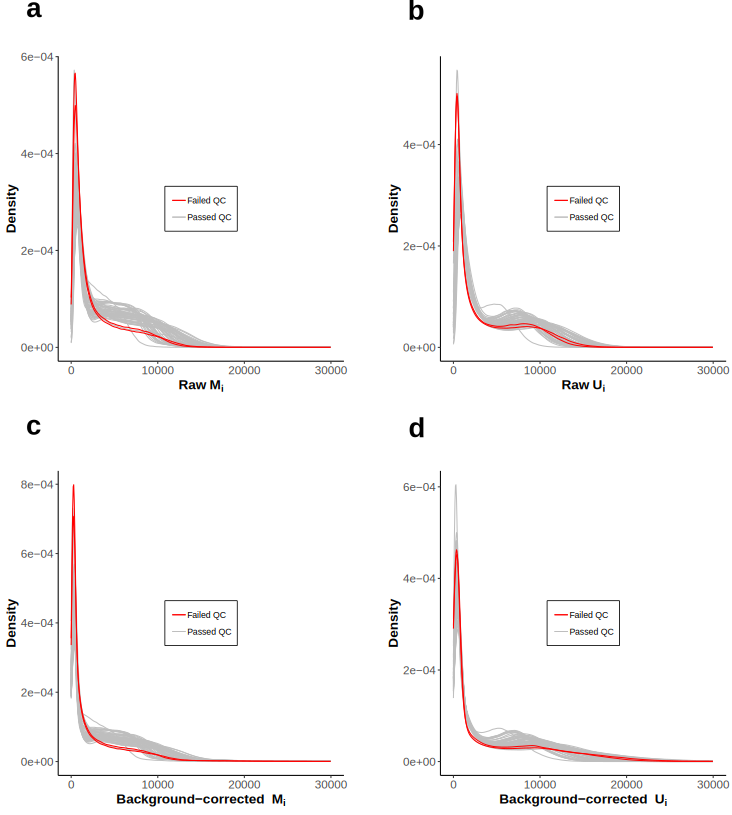
\includegraphics[width=0.62\textwidth]{SC2_Fig1}
	\caption[Effects of \textit{noob} background correction on the array fluorescence intensities.]{Effects of \textit{noob} background correction on the array flurescence intensities. Distributions of the array fluorescence intensities for the \textbf{a.} methylated signals ($M_{i}$) before background correction; \textbf{b.} unmethylated signals ($U_{i}$) before background correction; \textbf{c.} methylated signals ($M_{i}$) after background correction and \textbf{d.} unmethylated signals ($U_{i}$) after background correction. Each curve represents a DNA methylation sample from the GSE41273 batch. In grey: 51 samples that passed quality control (QC). In red: 2 samples that failed QC.}
	\label{fig:sc2_fig1}
\end{figure}

\begin{figure}[htbp!] 
	\centering    
	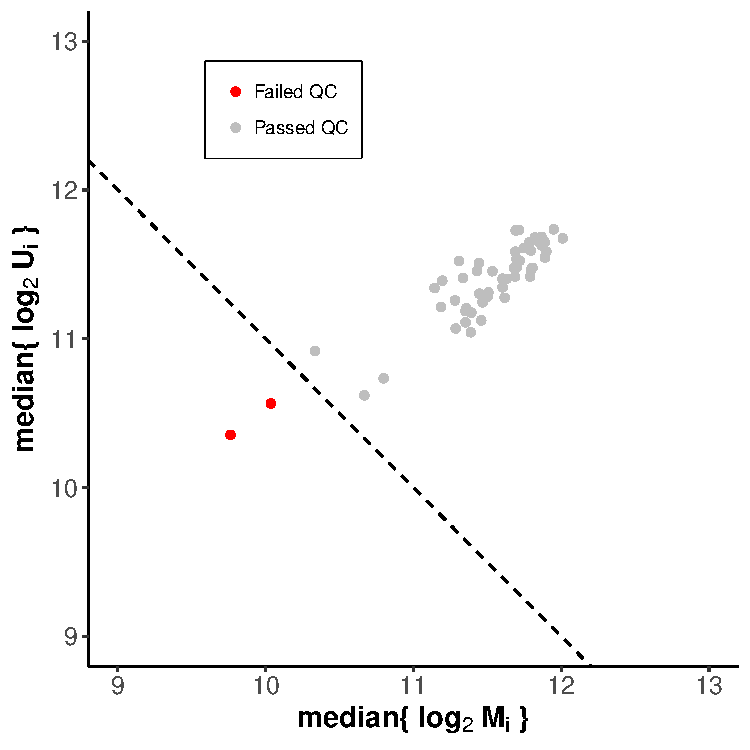
\includegraphics[width=0.5\textwidth]{SC2_Fig2}
	\caption[Quality control (QC) strategy to identify outlier samples.]{Quality control (QC) strategy to identify outlier samples, according to their global intensity values, in the GSE41273 batch. Those samples with low median intensity values (see criteria in section~\ref{s:2.1.2}) were discarded from downstream analyses (2/53, in red). Each sample is represented by one point. The dashed line represents the  intensity threshold. $M_{i}$ and $U_{i}$ represent the background-corrected methylated and unmethylated intensity measurements for the different 450K array probes in a given sample.}
	\label{fig:sc2_fig2}
\end{figure}

\begin{figure}[htbp!] 
	\centering    
	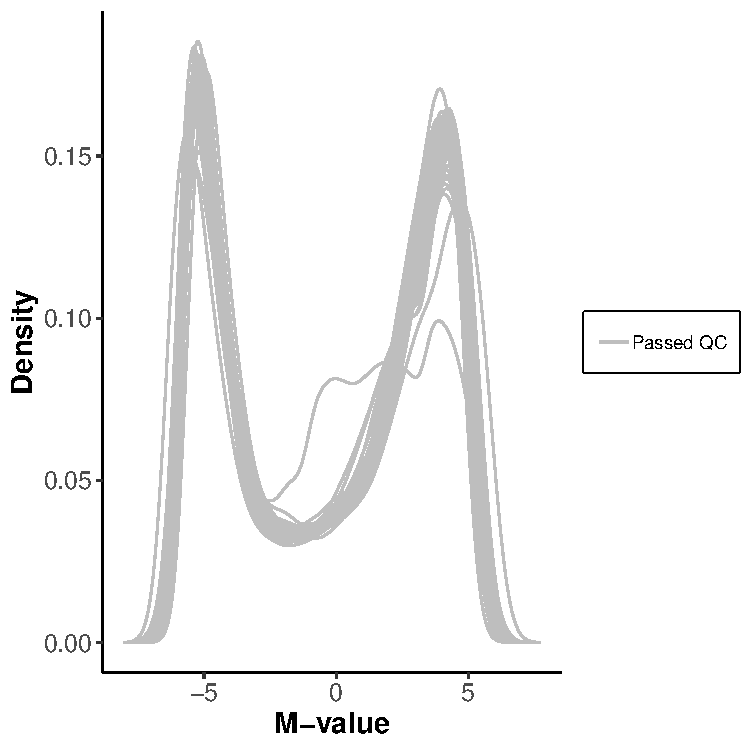
\includegraphics[width=0.5\textwidth]{SC2_Fig3}
	\caption[M-value distributions in the GSE41273 batch]{M-value distributions in the samples of the GSE41273 batch, after all the pre-processing steps have been carried out (background correction, quality control, probe filtering and BMIQ normalisation). M-values were calculated applying the logistic transformation to the $\beta$-values, as described in Du \textit{et al.} \cite{Du2010}. Each curve represents a different sample.}
	\label{fig:sc2_fig3}
\end{figure}

\begin{figure}[htbp!] 
	\centering    
	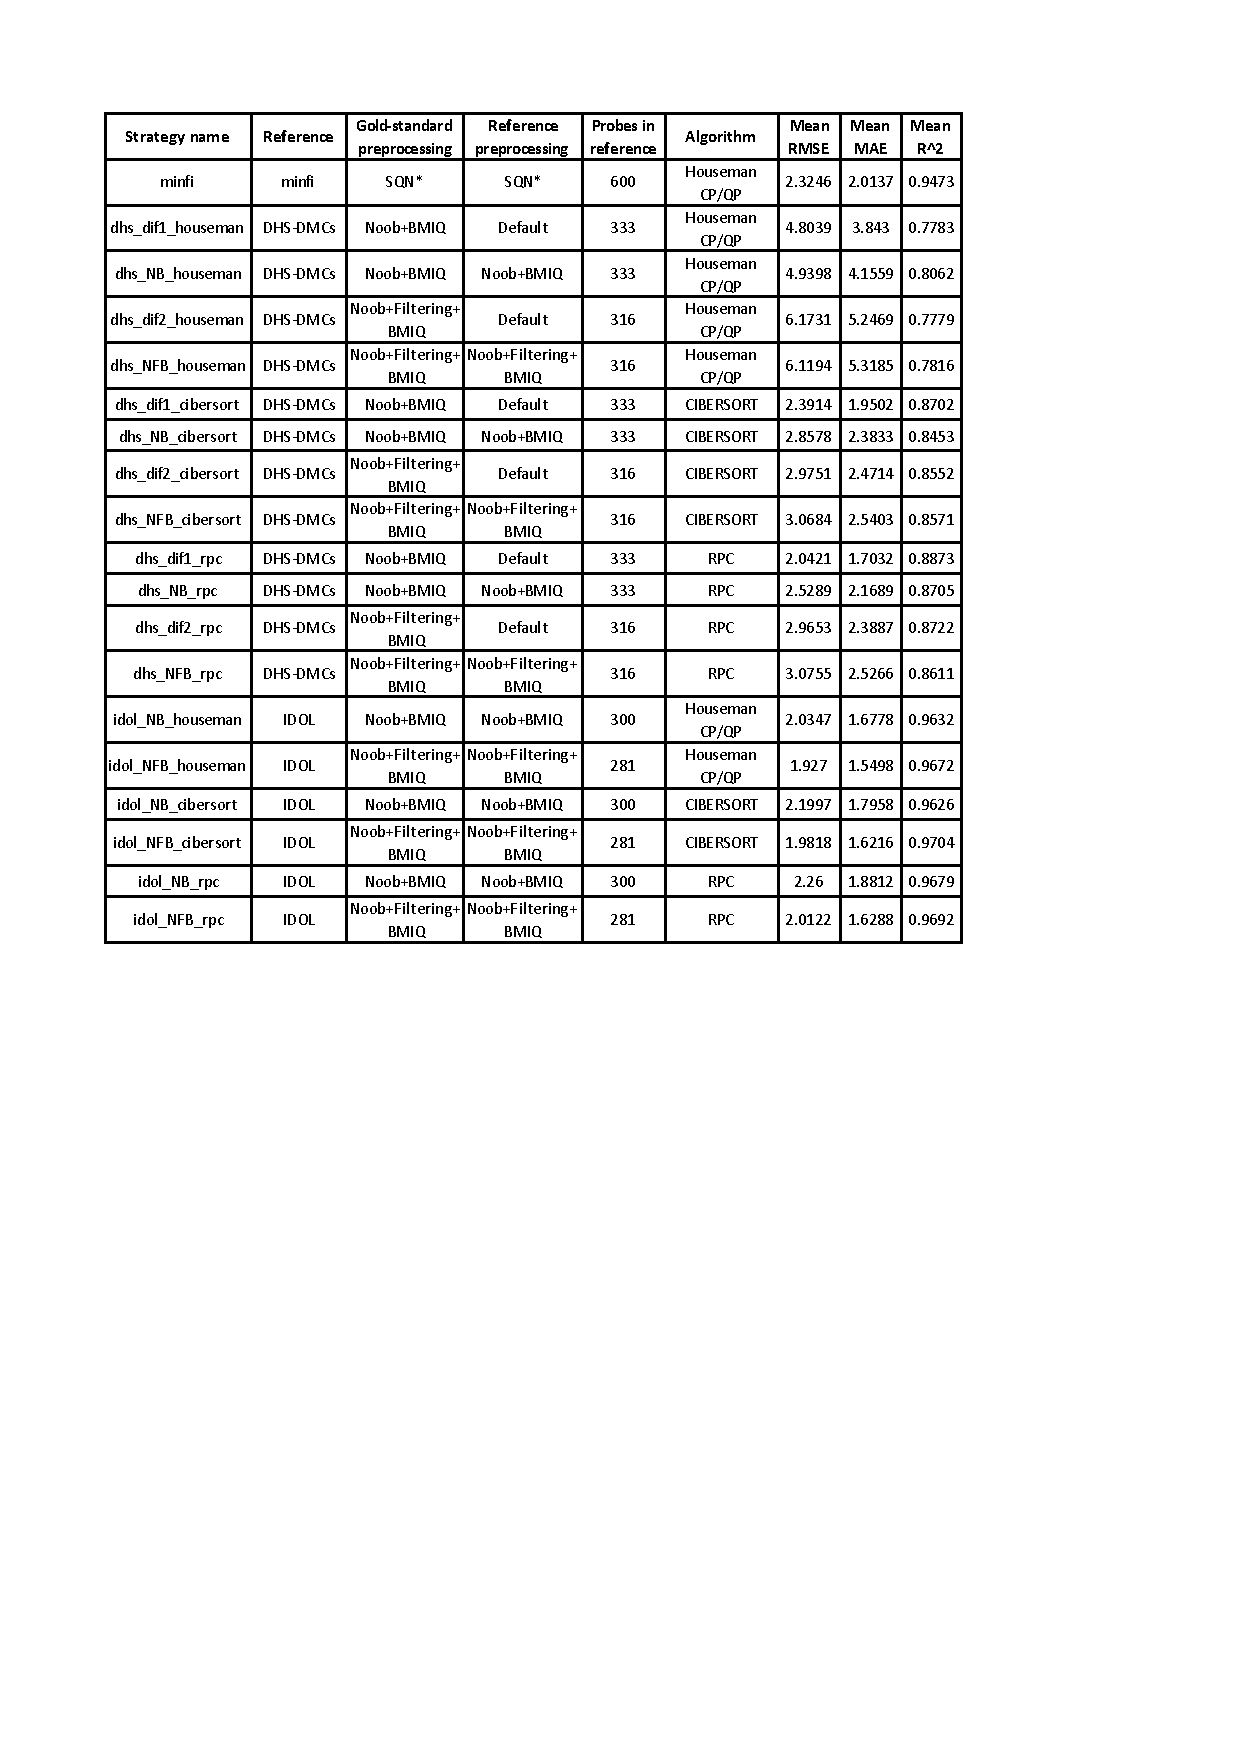
\includegraphics[width=1\textwidth]{SC2_Fig4}
	\caption[Cell-type deconvolution strategies that were benchmarked]{Table showing the different cell-type deconvolution strategies that were benchmarked. BMIQ: beta-mixture quantile normalisation. \acrshort{CP/QP}: constrained projection/quadratic programming. \acrshort{MAE}: mean absolute error. Noob: \textit{noob} background correction.  \acrshort{R$^2$}: coefficient of determination. \acrshort{RMSE}: root mean squared error. \acrshort{RPC}: robust partial correlations. \acrshort{SQN}: stratified quantile normalisation. `Default' refers to the pre-processing strategy employed in the original DHS-DMCs publication, as implemented in the \textit{EpiDISH} R package (\textit{centDHSbloodDMC.m}) \cite{Teschendorff2017a,Teschendorff2017b}. See section~\ref{s:2.1.3} in the main text for more details on what the different references refer to.}
	\label{fig:sc2_fig4}
\end{figure}

\begin{figure}[htbp!] 
	\centering    
	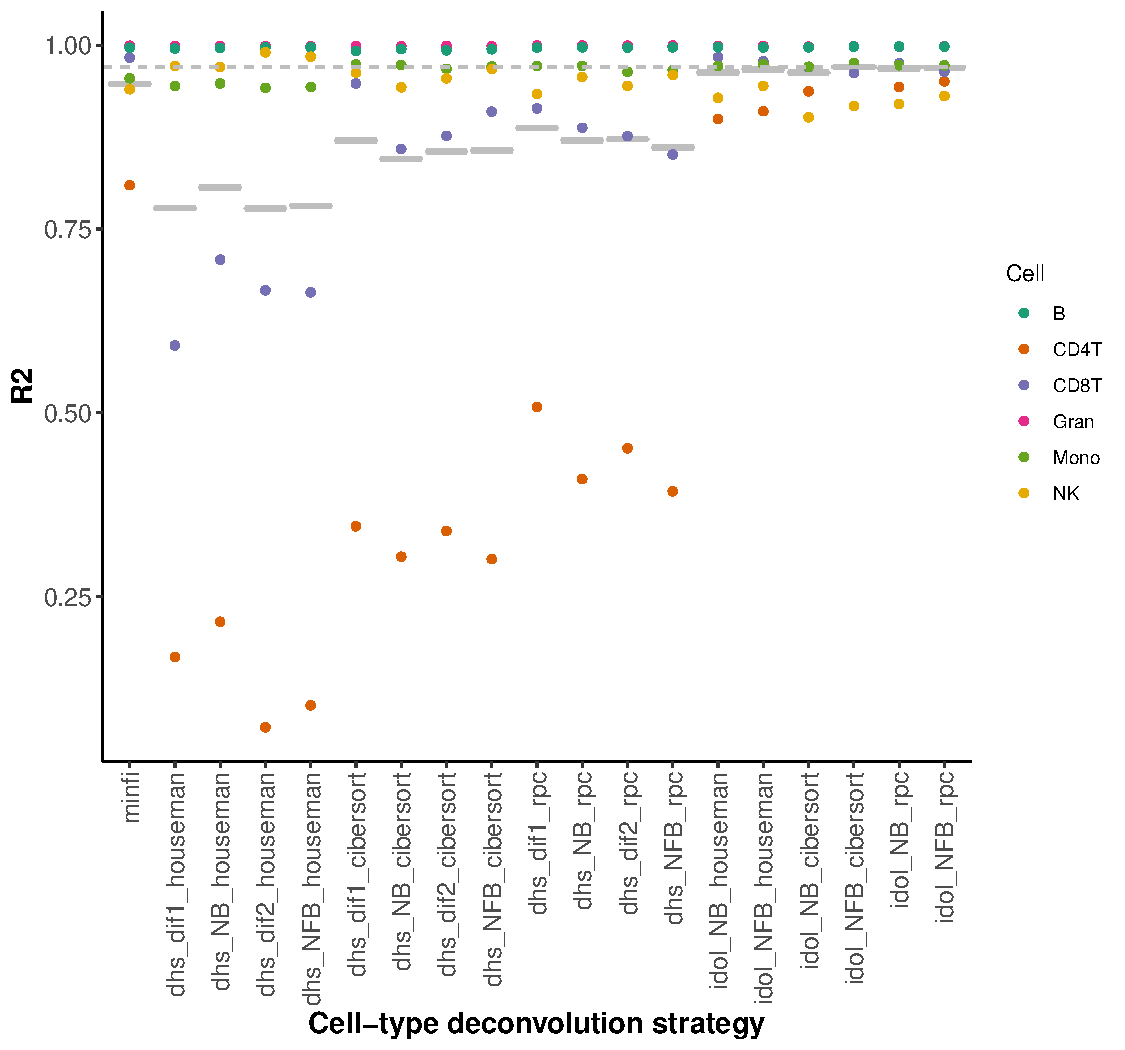
\includegraphics[width=1\textwidth]{SC2_Fig5}
	\caption[Benchmarking of the cell-type deconvolution strategies in blood: R$^2$]{Benchmarking of the cell-type deconvolution strategies in blood. The x-axis shows the different strategies that were tested (for a detailed description see Fig.~\ref{fig:sc2_fig4}). The y-axis shows the results for the coefficient of determination (R$^2$) when comparing the predictions with the real proportions of cells in a gold-standard dataset (GSE77797) \cite{Koestler2016}. The grey horizontal solid lines represent the mean for the R$^2$ across cell types and the grey dashed line the maximum of these values.}
	\label{fig:sc2_fig5}
\end{figure}

\begin{figure}[htbp!]
	\centering    
	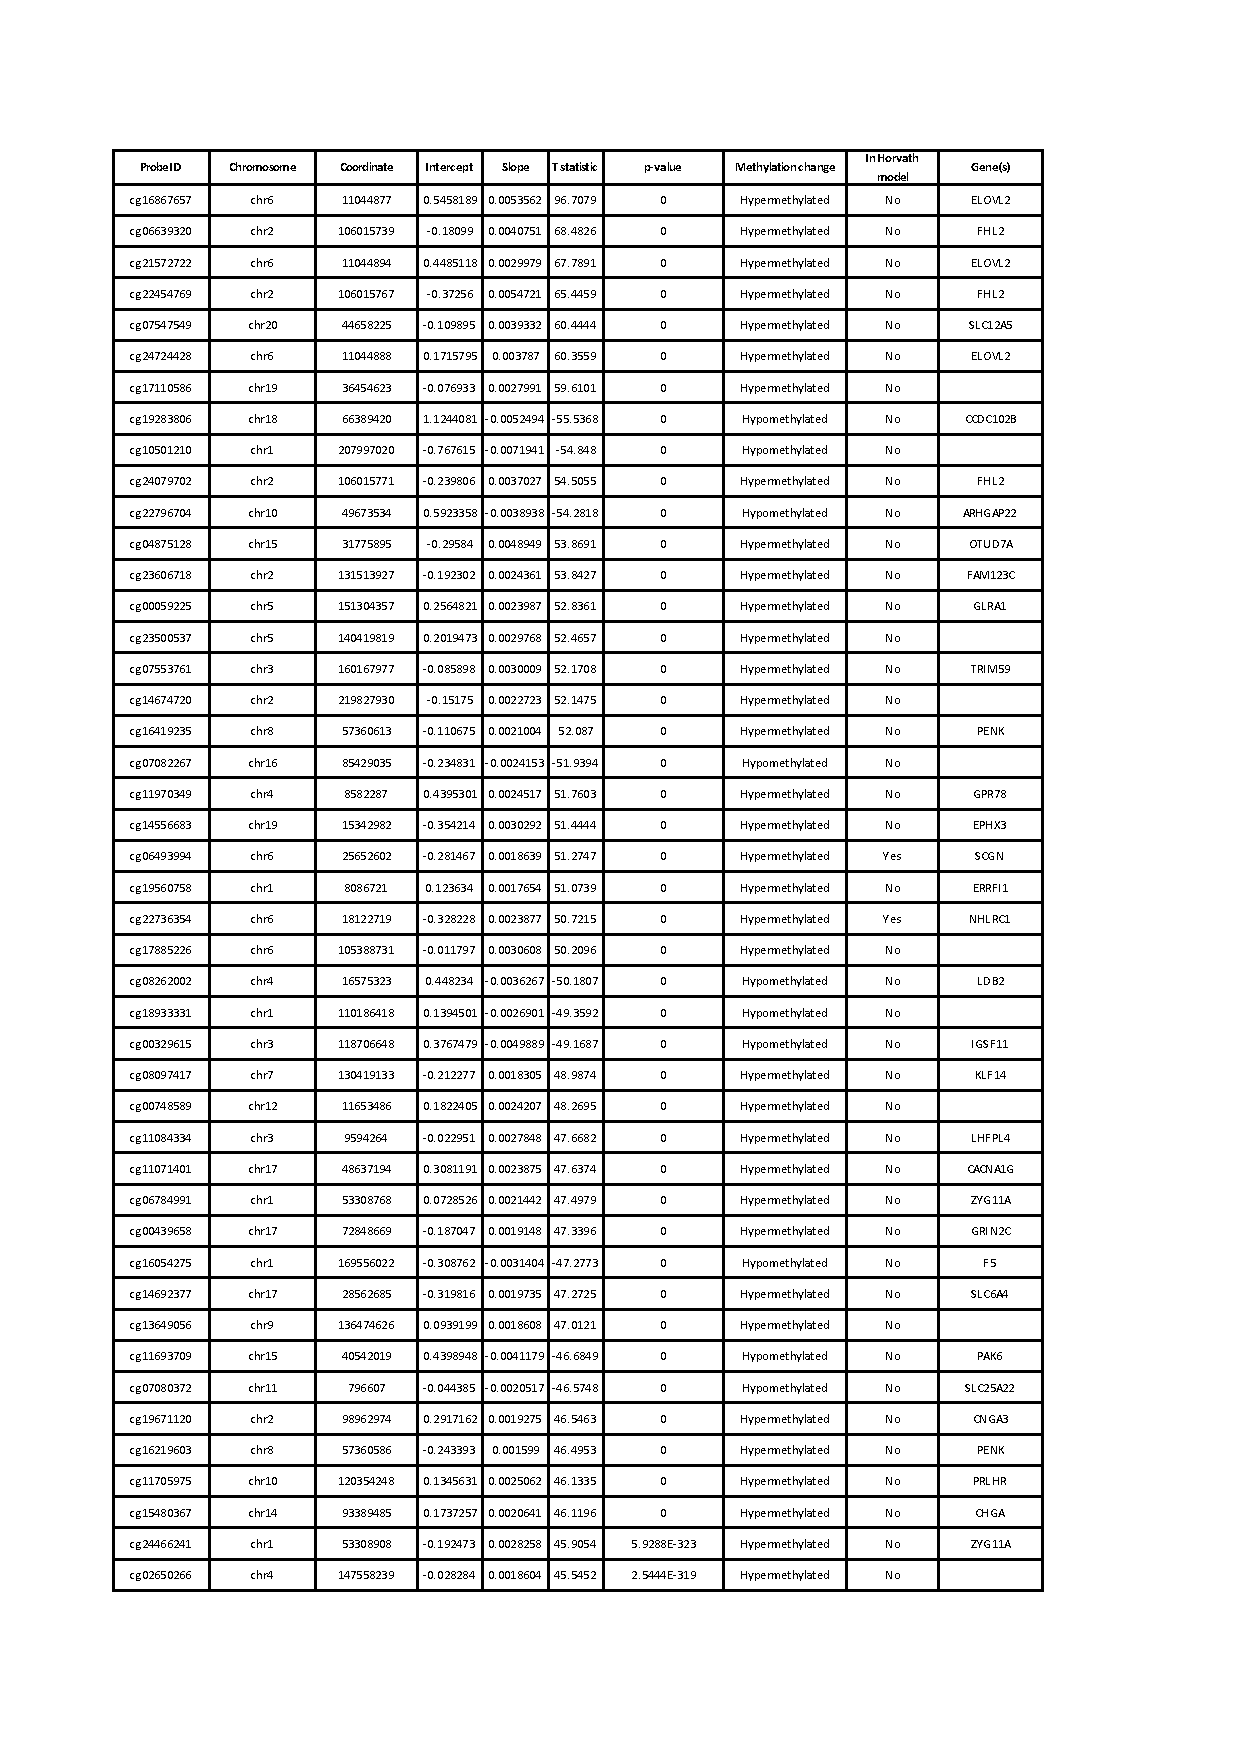
\includegraphics[width=1\textwidth]{SC2_Fig6_1}
\end{figure}
\begin{figure}[htbp!]
	\centering    
	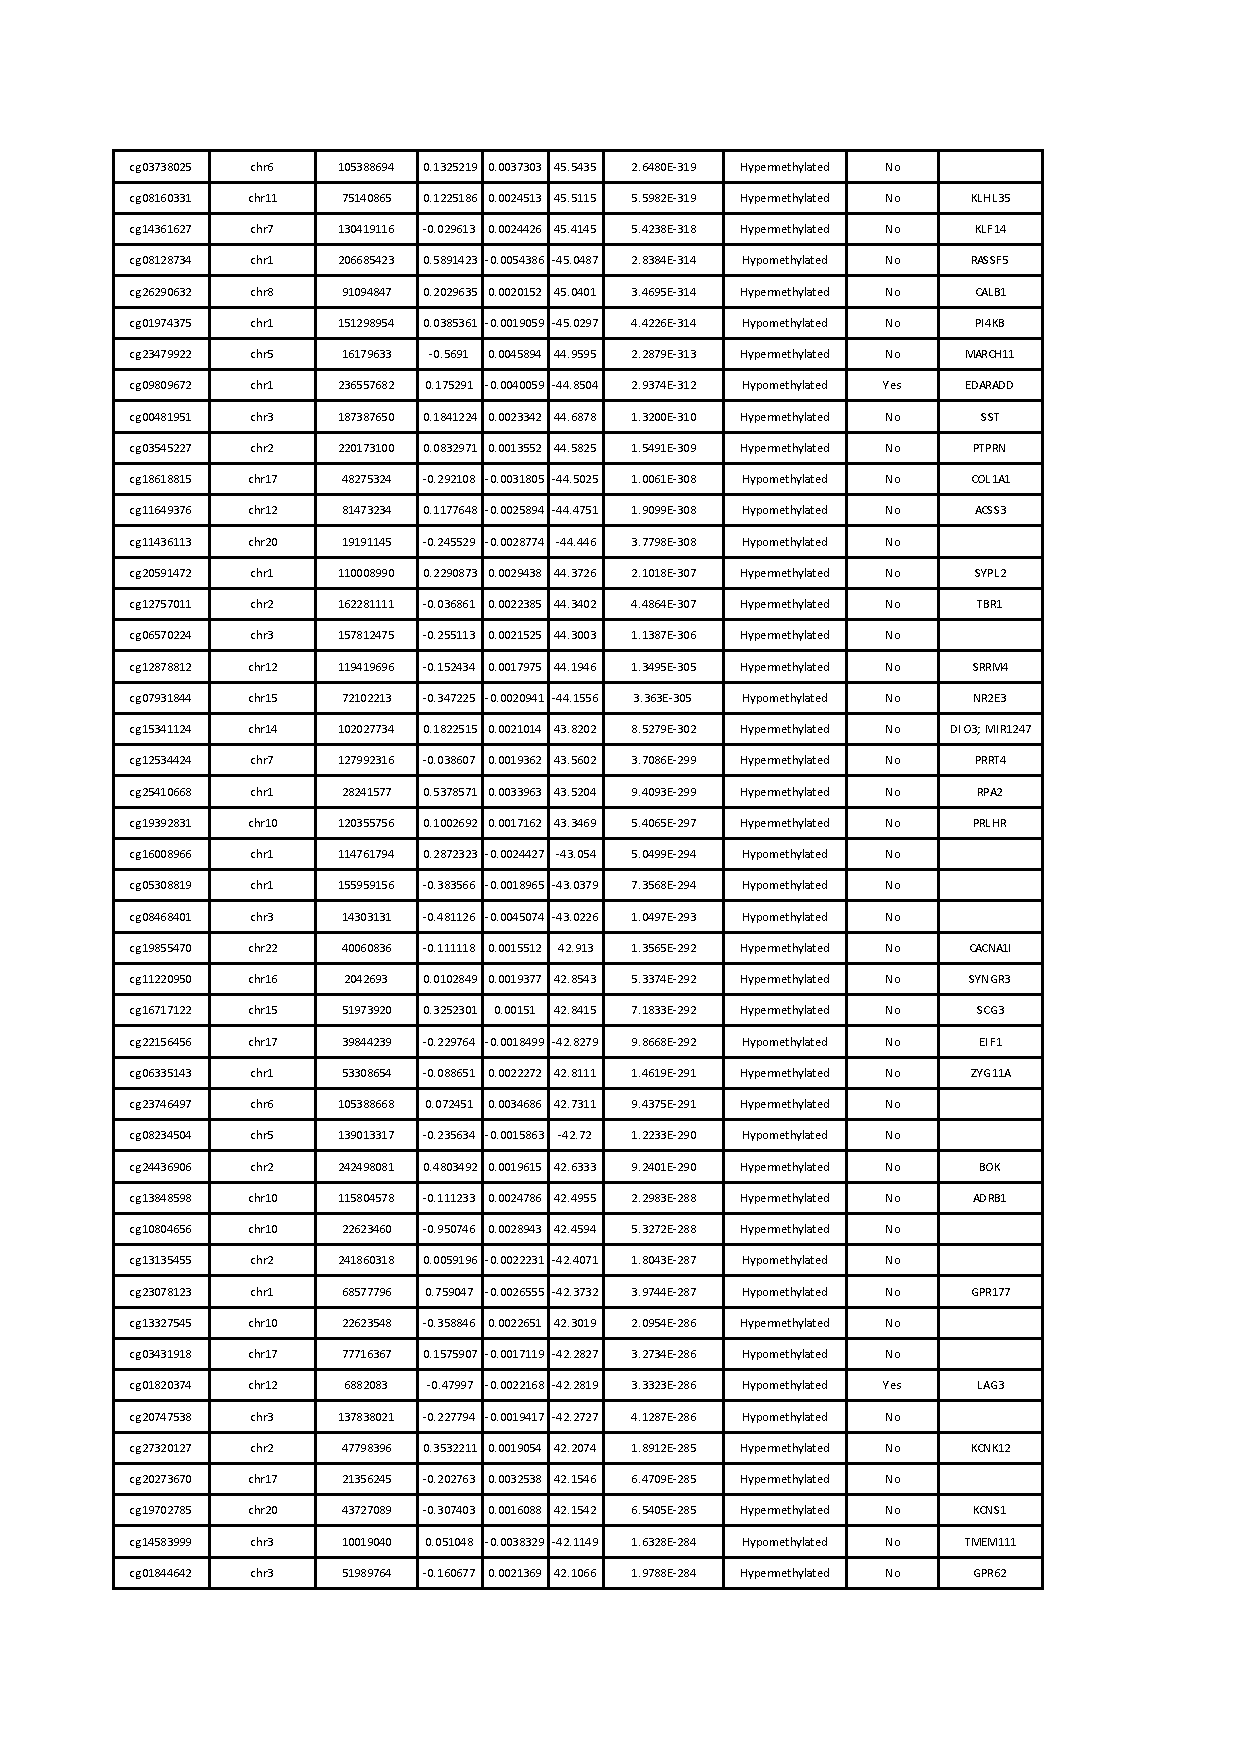
\includegraphics[width=1\textwidth]{SC2_Fig6_2}
\end{figure}
\begin{figure}[htbp!]
	\centering    
	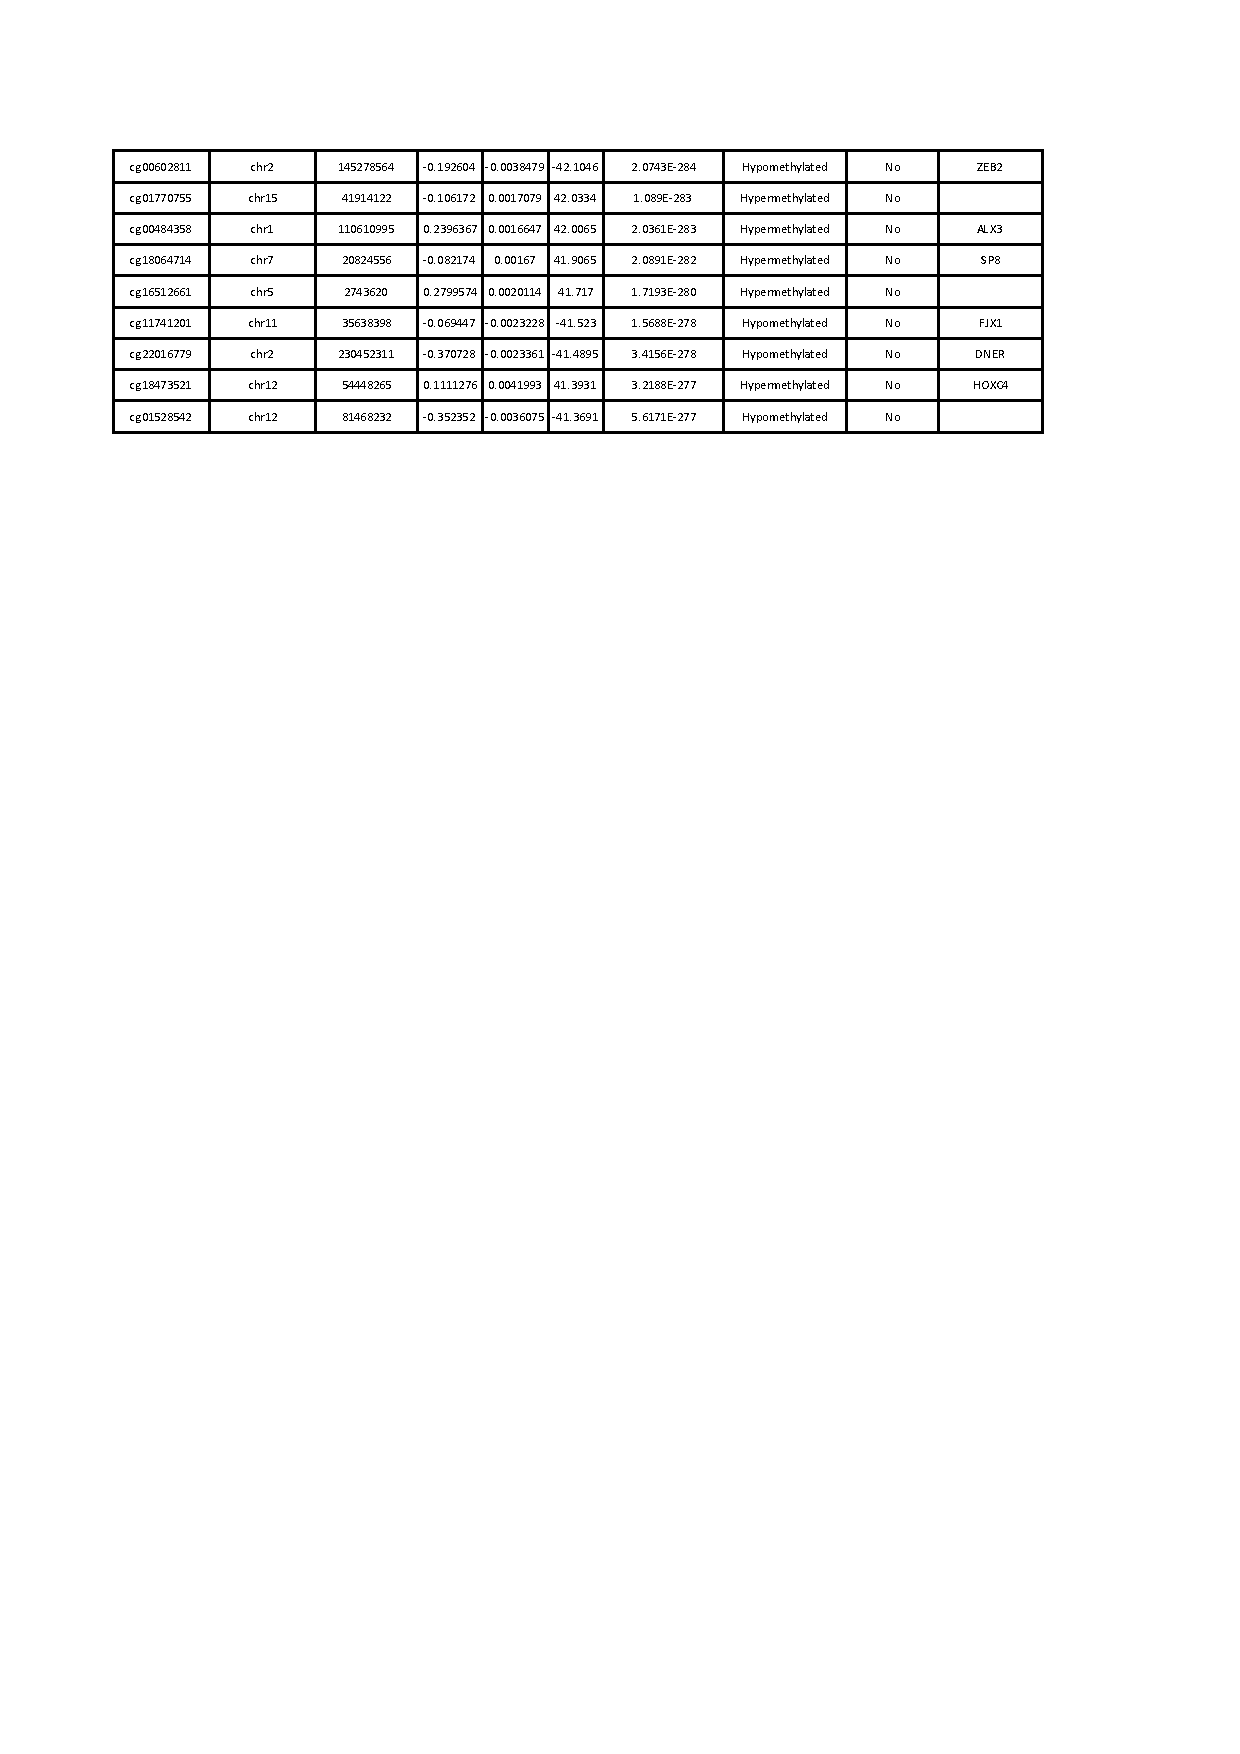
\includegraphics[width=1\textwidth]{SC2_Fig6_3}
	\caption[Table showing the top 100 aDMPs]{Table showing the characteristics of the top 100 differentially methylated positions during ageing (aDMPs) in the blood of the healthy individuals, ordered by p-value and the absolute value of the T statistic. The chromosome and coordinate refer to the \textit{hg19} human genome assembly. The reported genes are the closest genes associated with the array probe, as specified by the 450K array annotation. In this case, cell composition correction (CCC) was applied during modelling (see section~\ref{s:2.1.4}).}
	\label{fig:sc2_fig6}
\end{figure}	

\begin{figure}[htbp!] 
	\centering    
	\vspace*{3mm}
	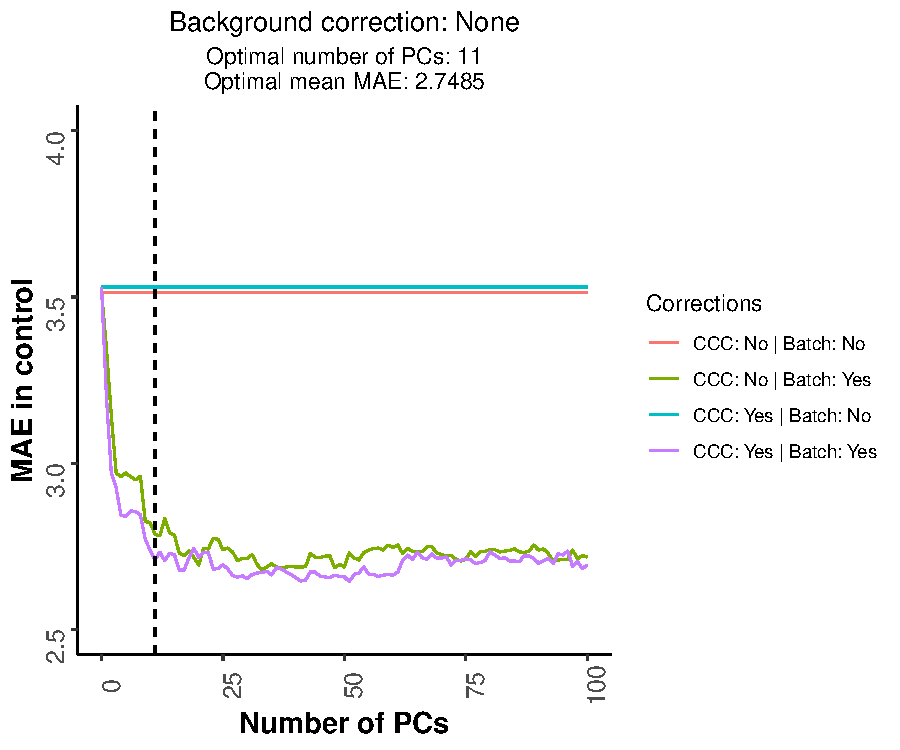
\includegraphics[width=0.8\textwidth]{SC2_Fig7}
	\caption[Impact of the absence of background correction on the predictions from the epigenetic clock]{Plot showing how the median absolute error (MAE) of the prediction in the healthy individual samples, that should tend to zero, is reduced when the PCs capturing the technical variation are included as part of the modelling strategy (see equations \ref{eq:2.16} and \ref{eq:2.17}). The dashed line represents the optimal number of PCs (11) that was finally used. The optimal mean MAE is calculated as the average MAE between the green and purple lines. In this case, no background correction was applied to the methylation data before calculating the epigenetic ages according to Horvath's epigenetic clock \cite{Horvath2013}.}
	\label{fig:sc2_fig7}
\end{figure}

\begin{figure}[htbp!] 
	\centering    
	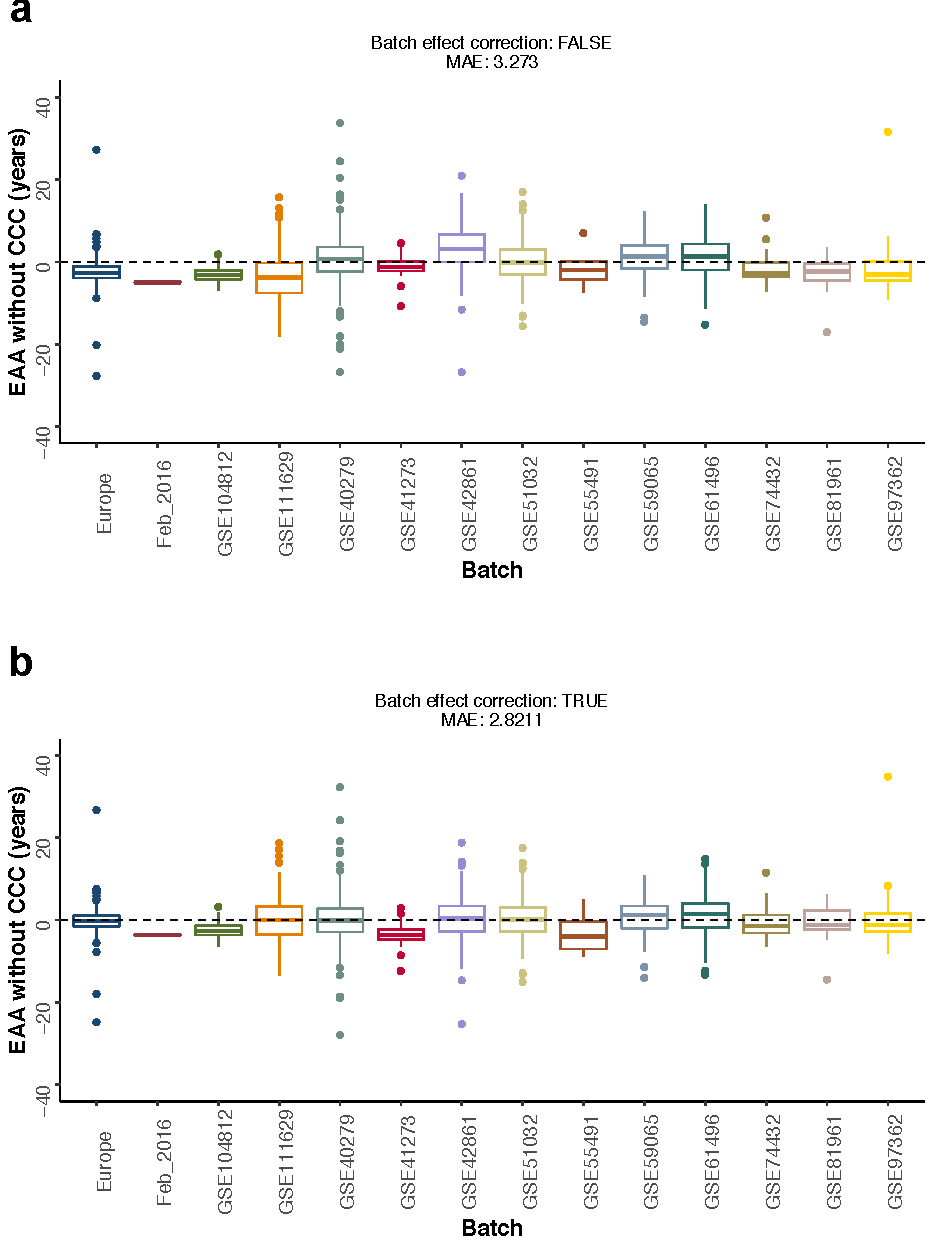
\includegraphics[width=0.9\textwidth]{SC2_Fig8}
	\caption[Correcting for batch effects: control model without cell composition correction]{Correcting for batch effects in the context of the epigenetic clock. \textbf{a.} Distribution of the epigenetic age acceleration (EAA) for the different batches of healthy individual samples, using the control model without cell composition correction (CCC) and before applying batch effect correction. The dashed black line represents $EAA = 0$, where the distributions should be centred around. \textbf{b.} As in a., but after applying batch effect correction (i.e. equivalent to equation \ref{eq:2.17}).}
	\label{fig:sc2_fig8}
\end{figure}

\begin{figure}[htbp!] 
	\centering    
	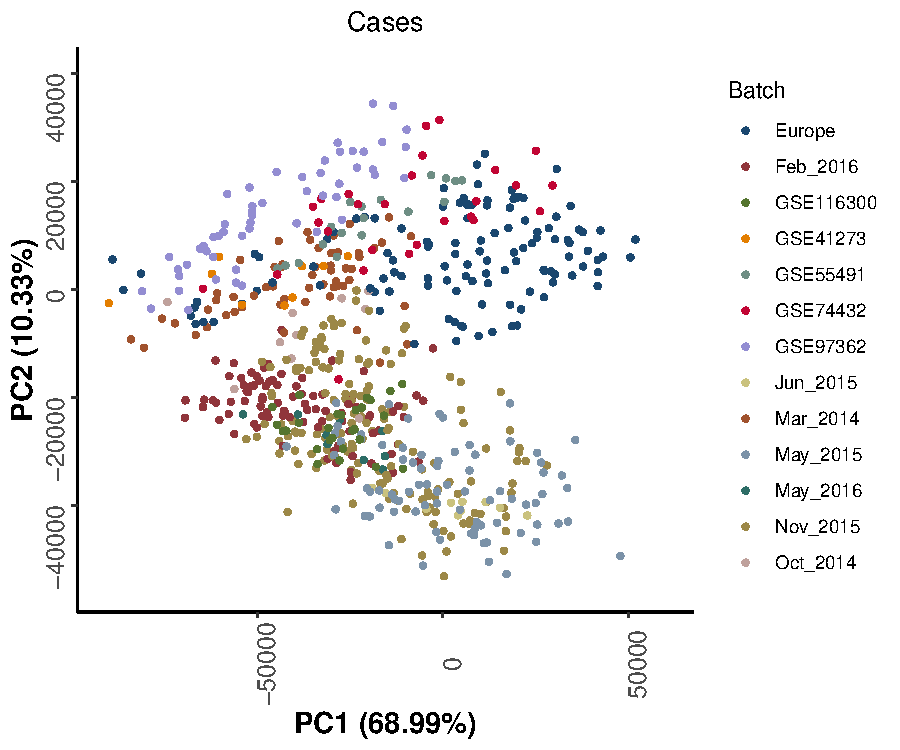
\includegraphics[width=0.7\textwidth]{SC2_Fig9}
	\caption[PCA on the array control probes captures batch effects: cases]{Scatterplot showing the values of the first two principal components (PCs) for the samples with developmental disorders (cases, see Chapter~\ref{c:3}) after performing PCA on the control probes of the 450K arrays. Each point corresponds to a different sample and the colours represent the different batches. The different batches cluster together in the PCA space, showing that the control probes indeed capture technical variation. Please note that all the PCA calculations were done using samples from both healthy individuals (full lifespan, $N=2218$) and cases from developmental disorders ($N=666$).}
	\label{fig:sc2_fig9}
\end{figure}

\begin{figure}[htbp!] 
	\vspace*{5mm}
	\centering    
	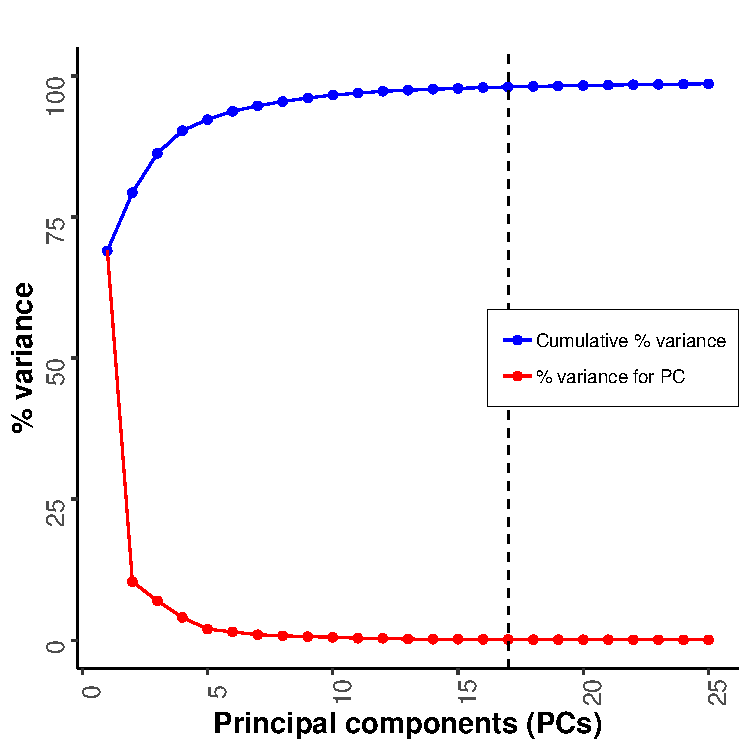
\includegraphics[width=0.5\textwidth]{SC2_Fig10}
	\caption[Variance explained by the different principal components during batch effect correction]{Plot showing the percentages of technical variance explained by the different PCs from the control probes. The dashed line represents the optimal number of PCs (17) that was finally used.}
	\label{fig:sc2_fig10}
\end{figure}

\clearpage

\renewcommand{\thesection}{S.2}   
\section{Biological aspects of the epigenetic clock}

\renewcommand\thefigure{S2.\arabic{figure}}
\renewcommand\thetable{S2.\arabic{table}}        
\vspace{10 mm}

\begin{table}[h]
	\centering
	\small
	\begin{tabular}{ p{2cm} p{1cm} p{1cm} p{1cm} p{2cm} p{6cm} }
		\toprule
		\textbf{Batch name} & \textbf{N$_{\female}$} & \textbf{N$_{\male}$} & \textbf{N} & \textbf{Median age (years)} & \textbf{Other comments} \\
		\midrule
		  Europe & 0 & 119 & 119 & 7.73 & \\
		  Feb\_2016 & 20 & 20 & 40 & 6 & \\
		  GSE116300 & 4 & 5 & 9 & 3 &\\
		  GSE41273 & 0 & 9 & 9 & 7.75 & \\
		  GSE74432 & 11 & 16 & 27 & 10 & \\
		  GSE97362 & 4 & 9 & 13 & 15 & Samples from the `validation cohort' were not included in the analysis, since they all seemed outliers on close examination\\
		  Jun\_2015 & 1 & 1 & 2 & 3.5015 & \\
		  Mar\_2014 & 11 & 6 & 17 & 8 & \\
		  May\_2015 & 17 & 49 & 66 & 14 & \\
		  Nov\_2015 & 35 & 30 & 65 & 6.7 & \\
		\midrule
		\textbf{Total} & 103 & 264 & 367 & 8 & - \\ 
		\bottomrule
	\end{tabular}
	\vspace*{3mm}
	\caption[Additional information for the developmental disorders dataset]{Overview of the blood DNA methylation dataset from individuals with developmental disorders. The batches `Europe', `Feb\_2016', `Jun\_2015', `Mar\_2014', `May\_2015' and `Nov\_2015' were generated in-house by our collaborators in Canada (see Chapter~\ref{c:3}). The rest of the batches were downloaded from GEO \cite{Edgar2002}. $N_{\female}$: number of samples from females. $N_{\male}$: number of samples from males. $N$: total number of samples. These numbers correspond to the samples left after applying quality control and filtering (see section~\ref{s:3.2}).}
	\label{table:s2_table1}
\end{table} 

\smallskip

\clearpage

\begin{figure}[htbp!]
	\setcounter{figure}{0}
	\centering    
	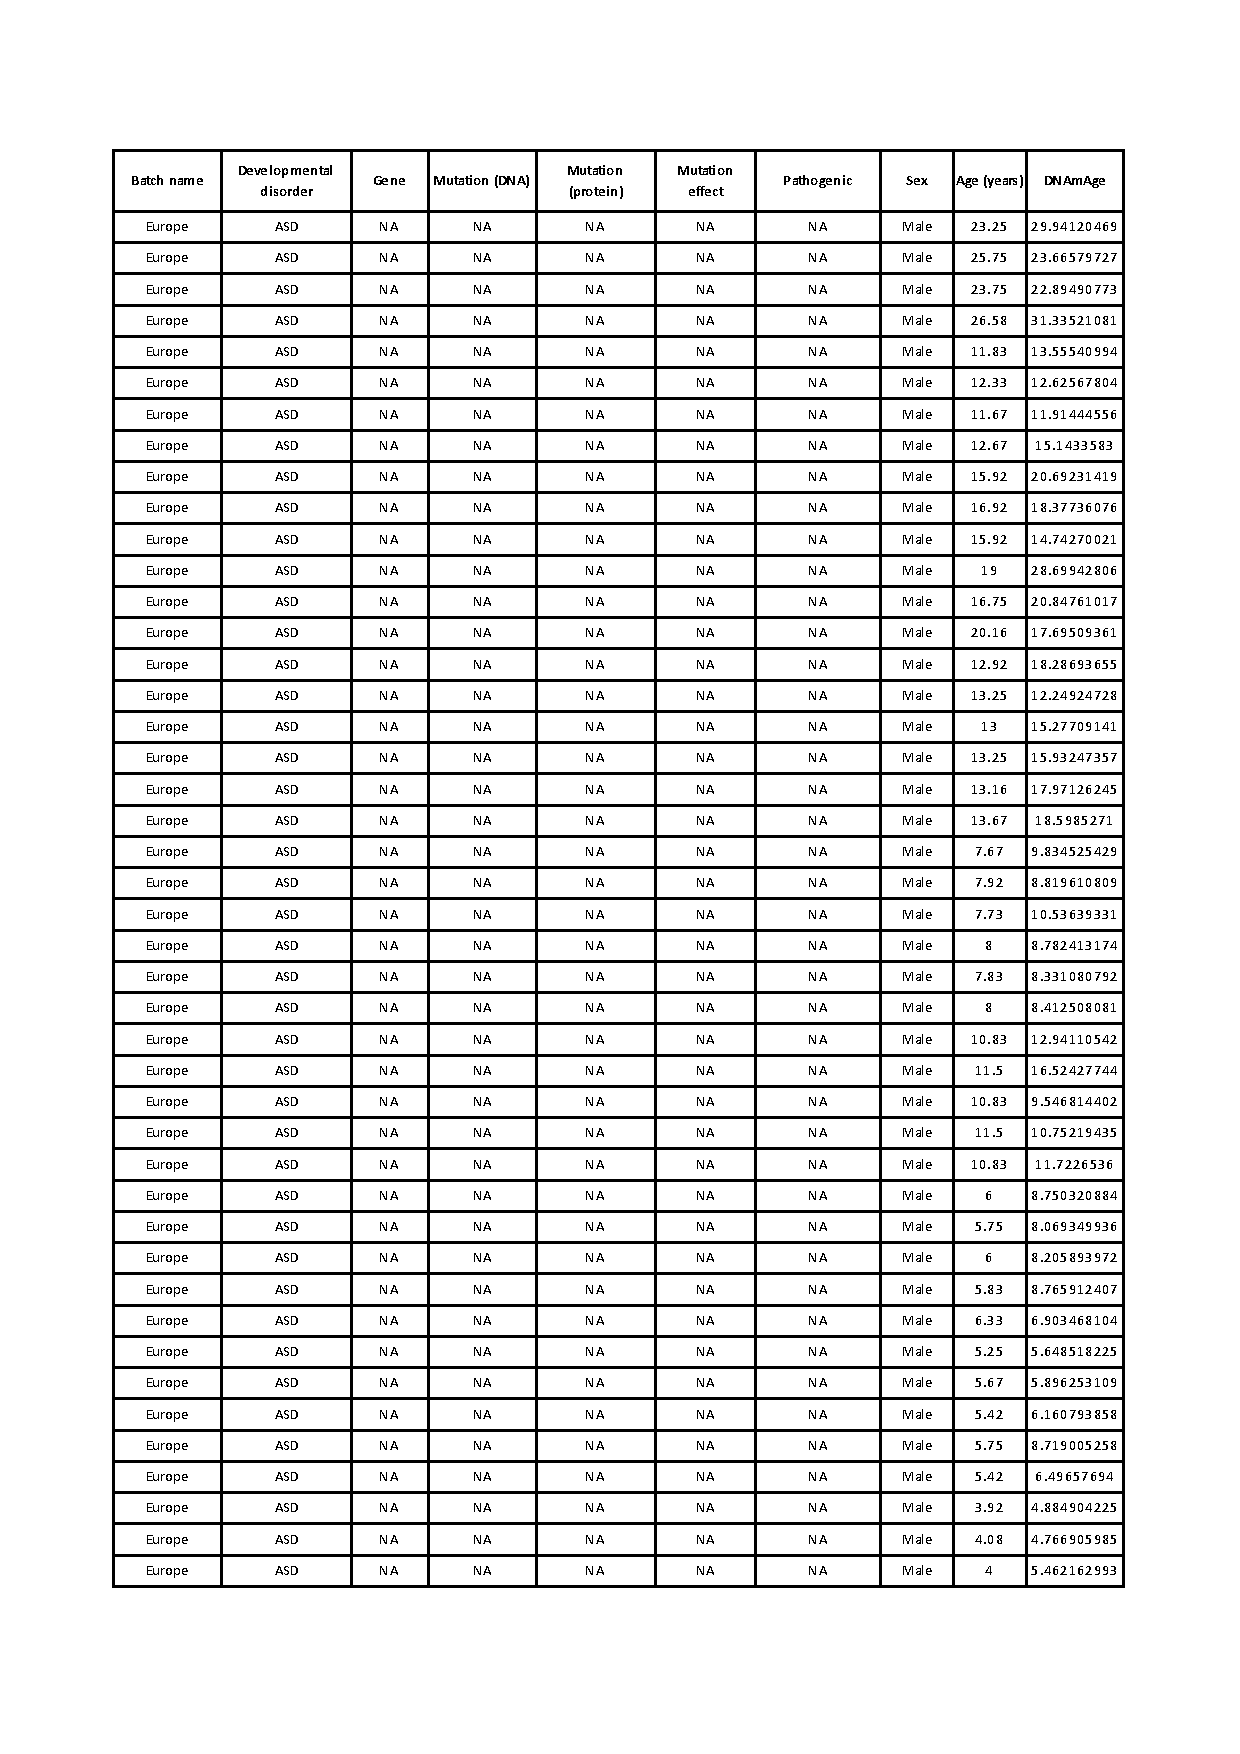
\includegraphics[width=1\textwidth]{SC3_Fig1_1}
\end{figure}
\begin{figure}[htbp!]
	\centering    
	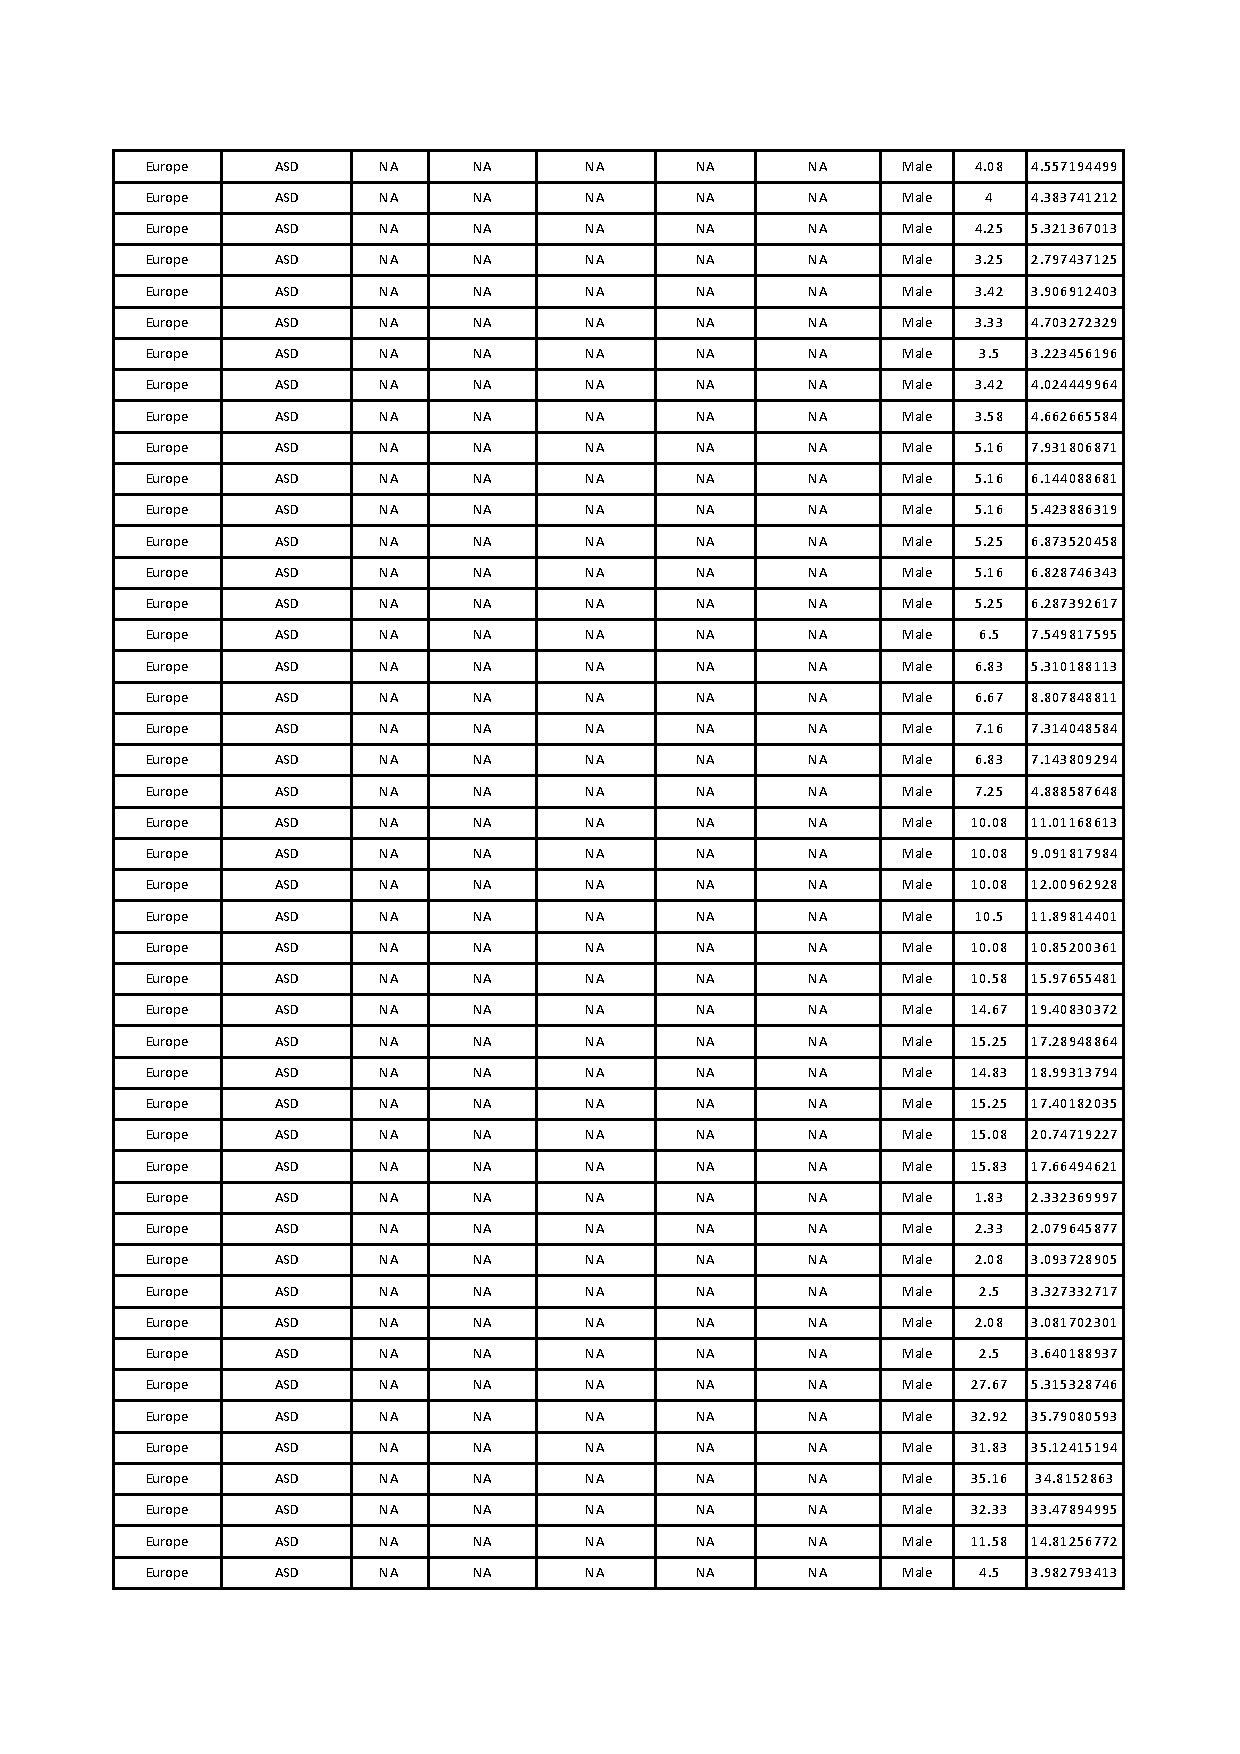
\includegraphics[width=1\textwidth]{SC3_Fig1_2}
\end{figure}
\begin{figure}[htbp!]
	\centering    
	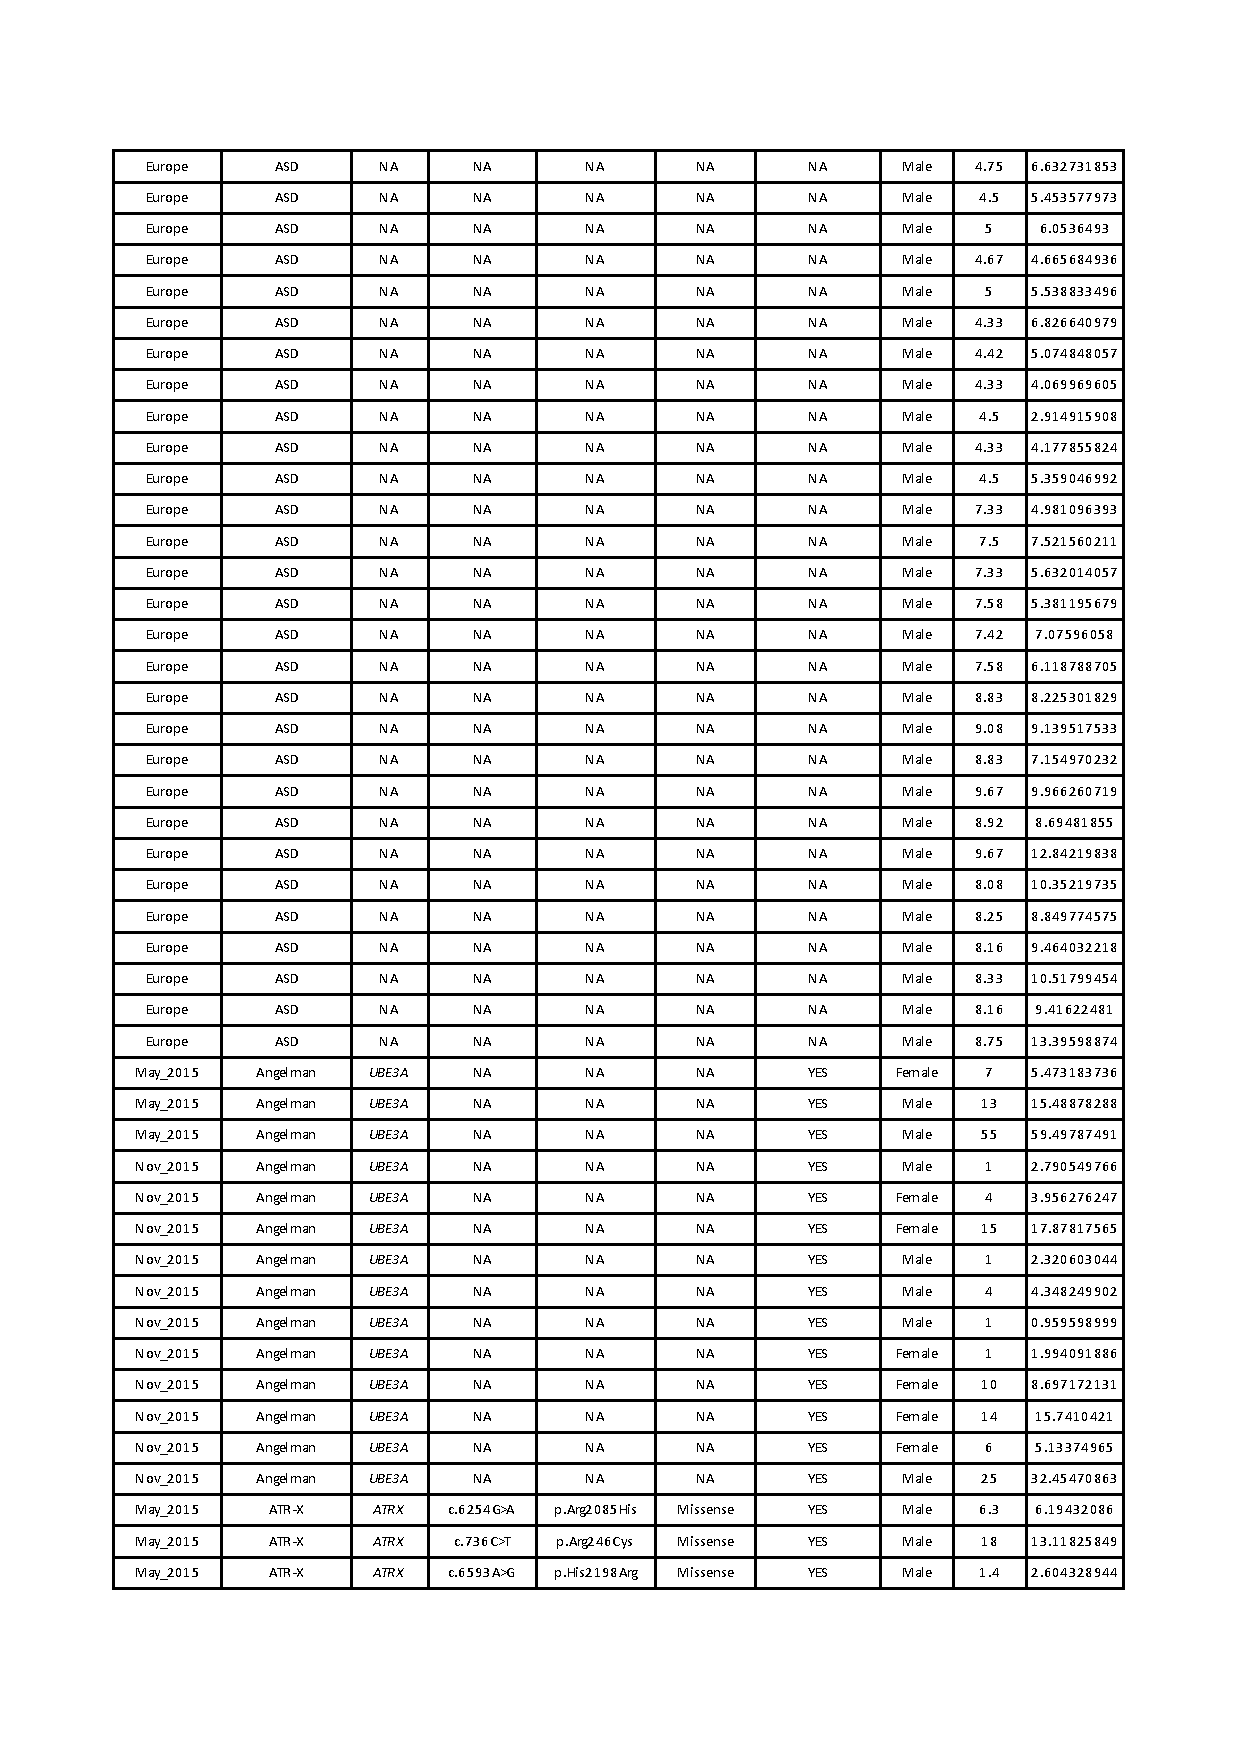
\includegraphics[width=1\textwidth]{SC3_Fig1_3}
\end{figure}
\begin{figure}[htbp!]
	\centering    
	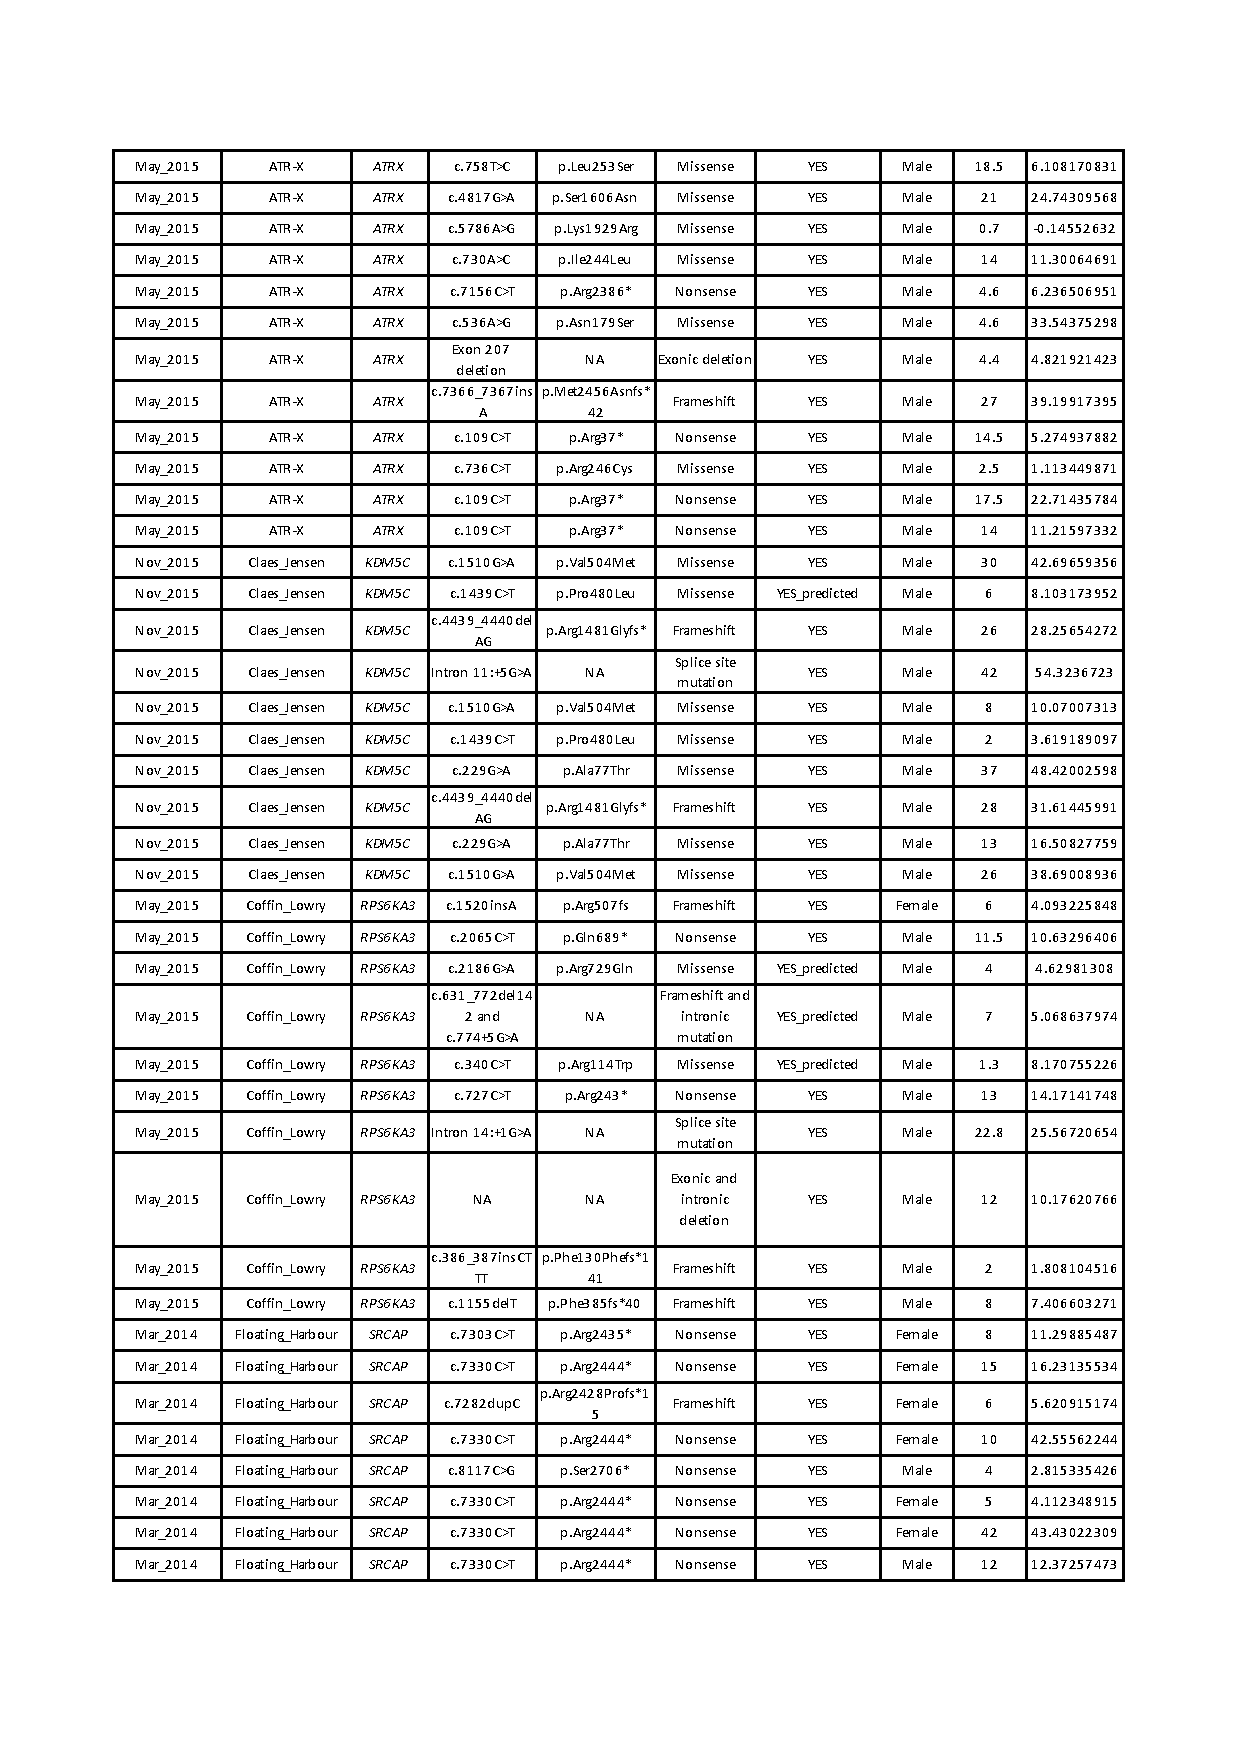
\includegraphics[width=1\textwidth]{SC3_Fig1_4}
\end{figure}
\begin{figure}[htbp!]
	\centering    
	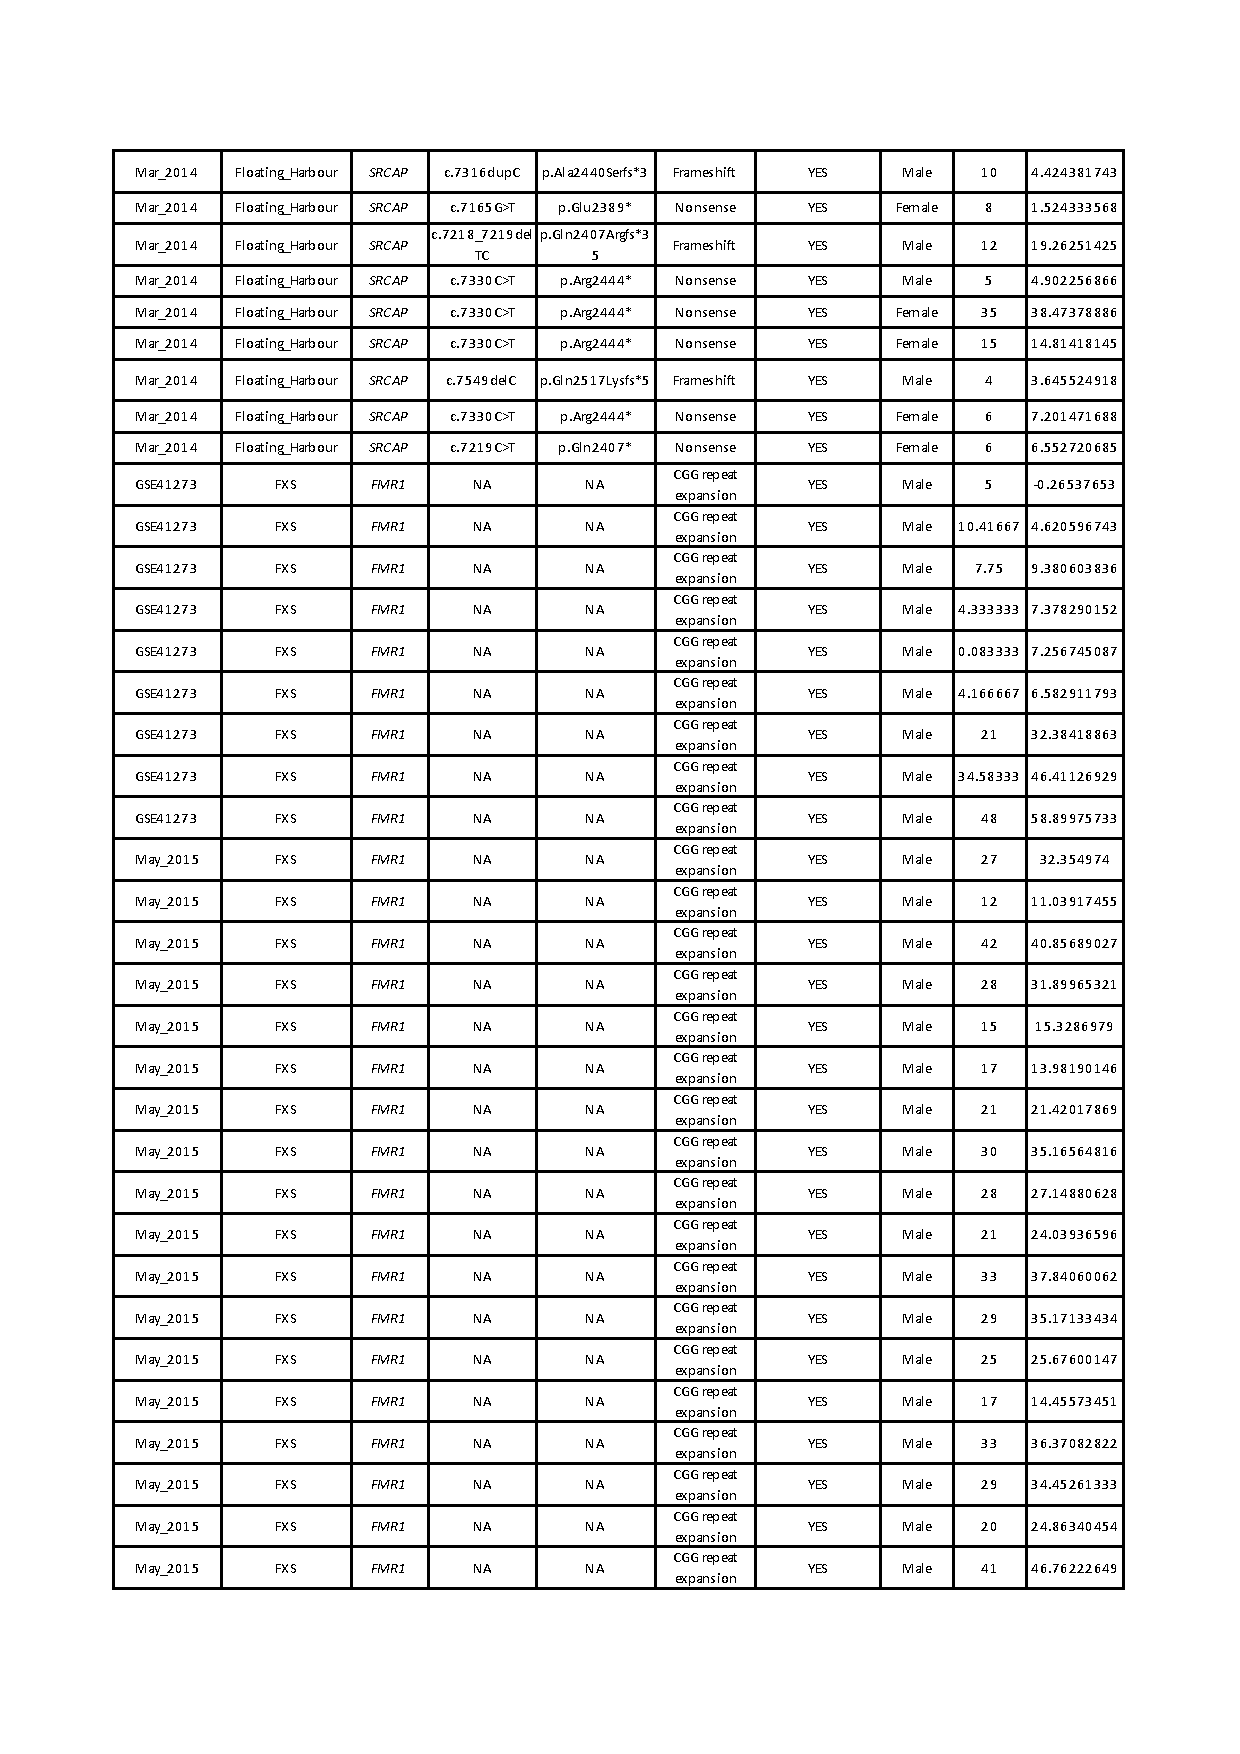
\includegraphics[width=1\textwidth]{SC3_Fig1_5}
\end{figure}
\begin{figure}[htbp!]
	\centering    
	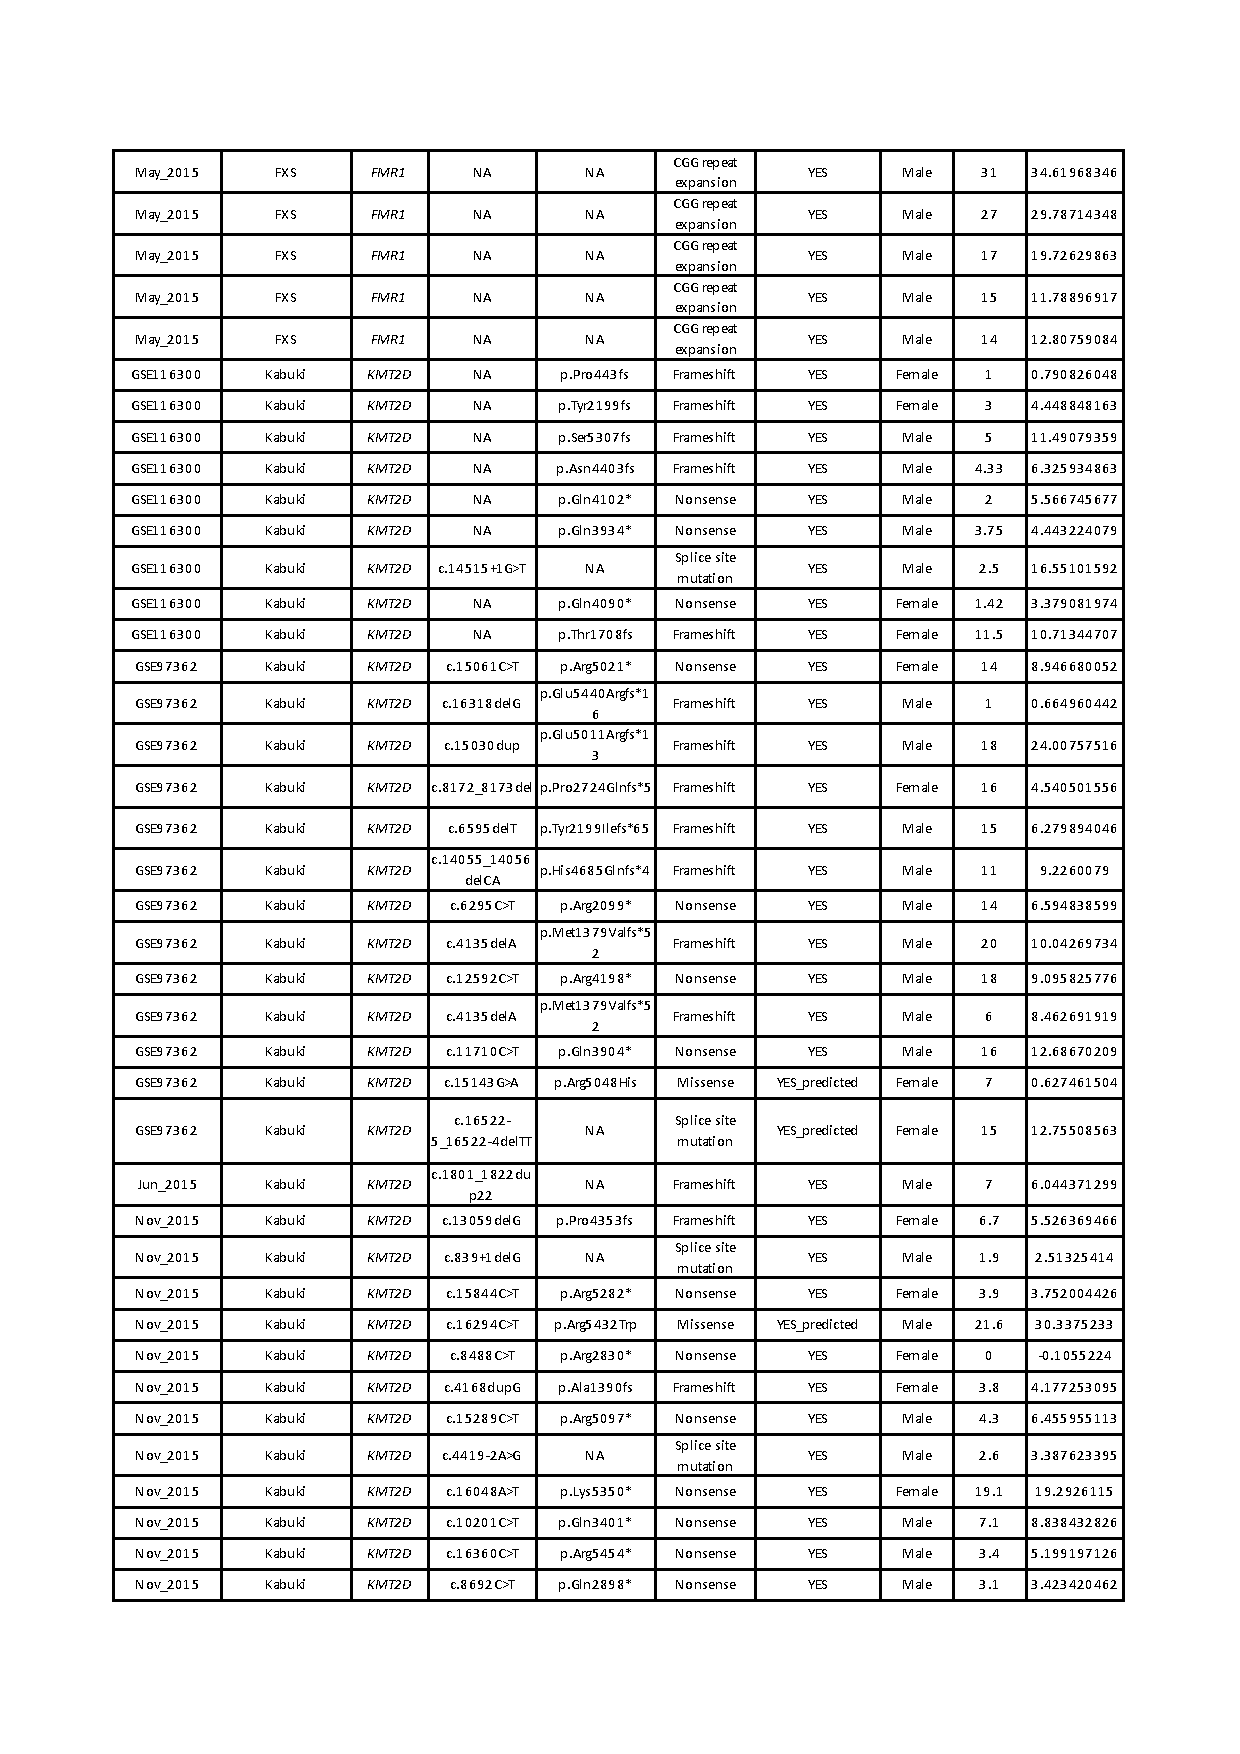
\includegraphics[width=1\textwidth]{SC3_Fig1_6}
\end{figure}
\begin{figure}[htbp!]
	\centering    
	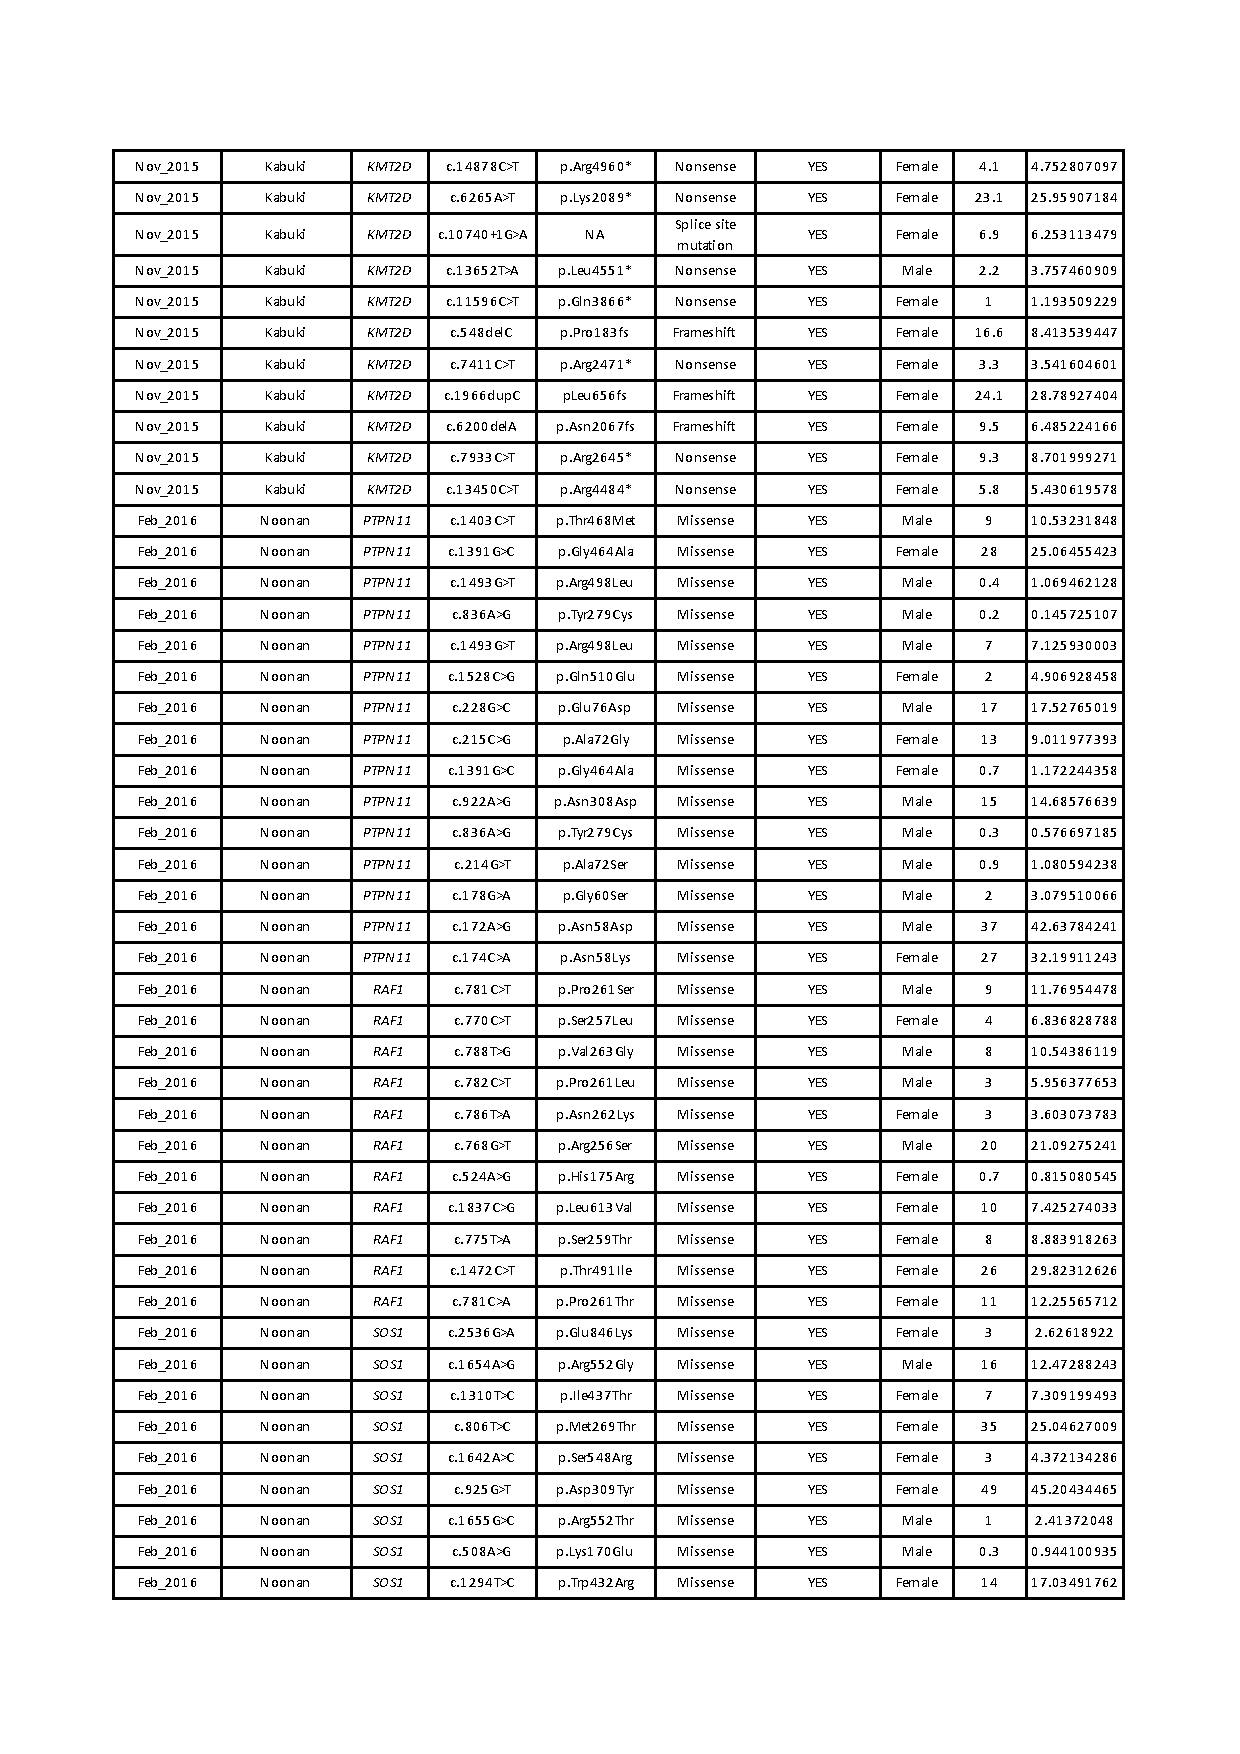
\includegraphics[width=1\textwidth]{SC3_Fig1_7}
\end{figure}
\begin{figure}[htbp!]
	\centering    
	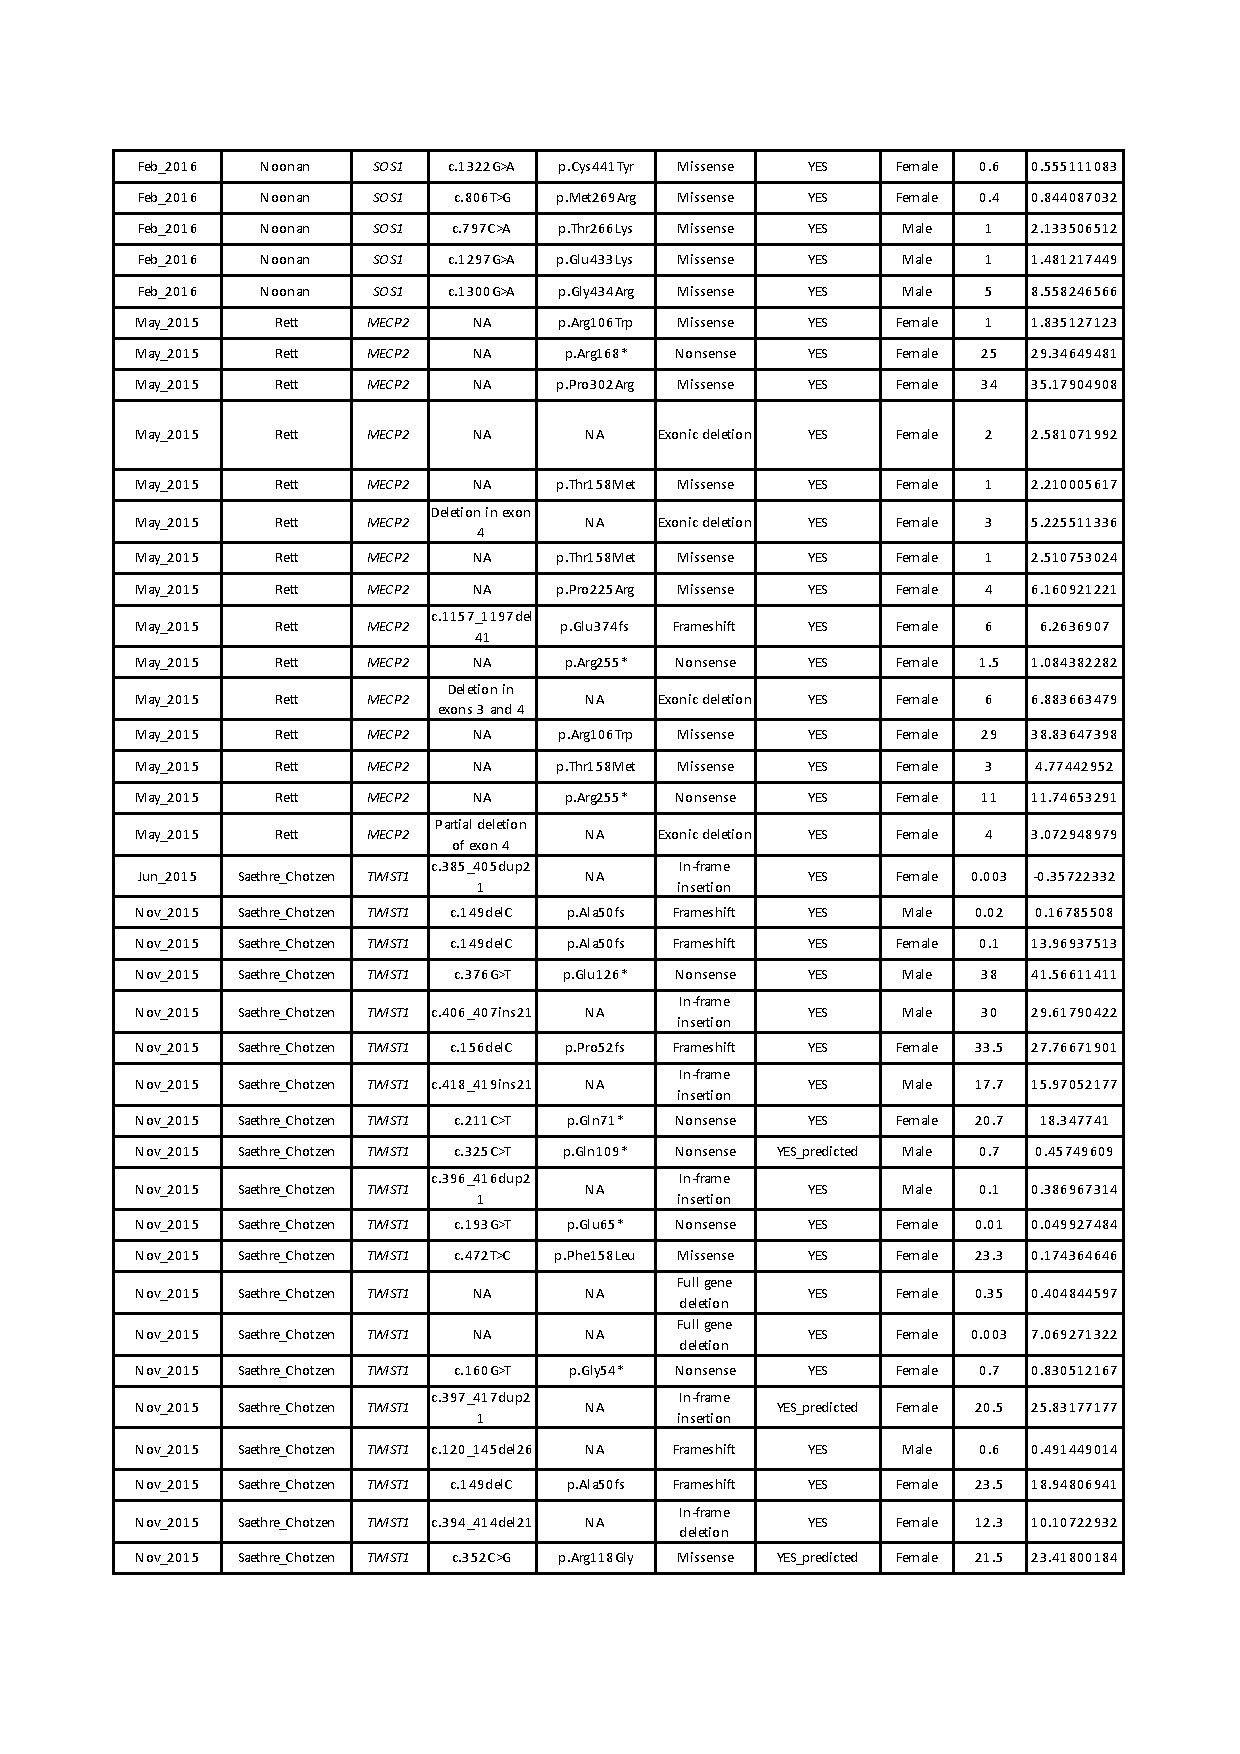
\includegraphics[width=1\textwidth]{SC3_Fig1_8}
\end{figure}
\begin{figure}[htbp!]
	\centering
	\vspace*{-40mm}    
	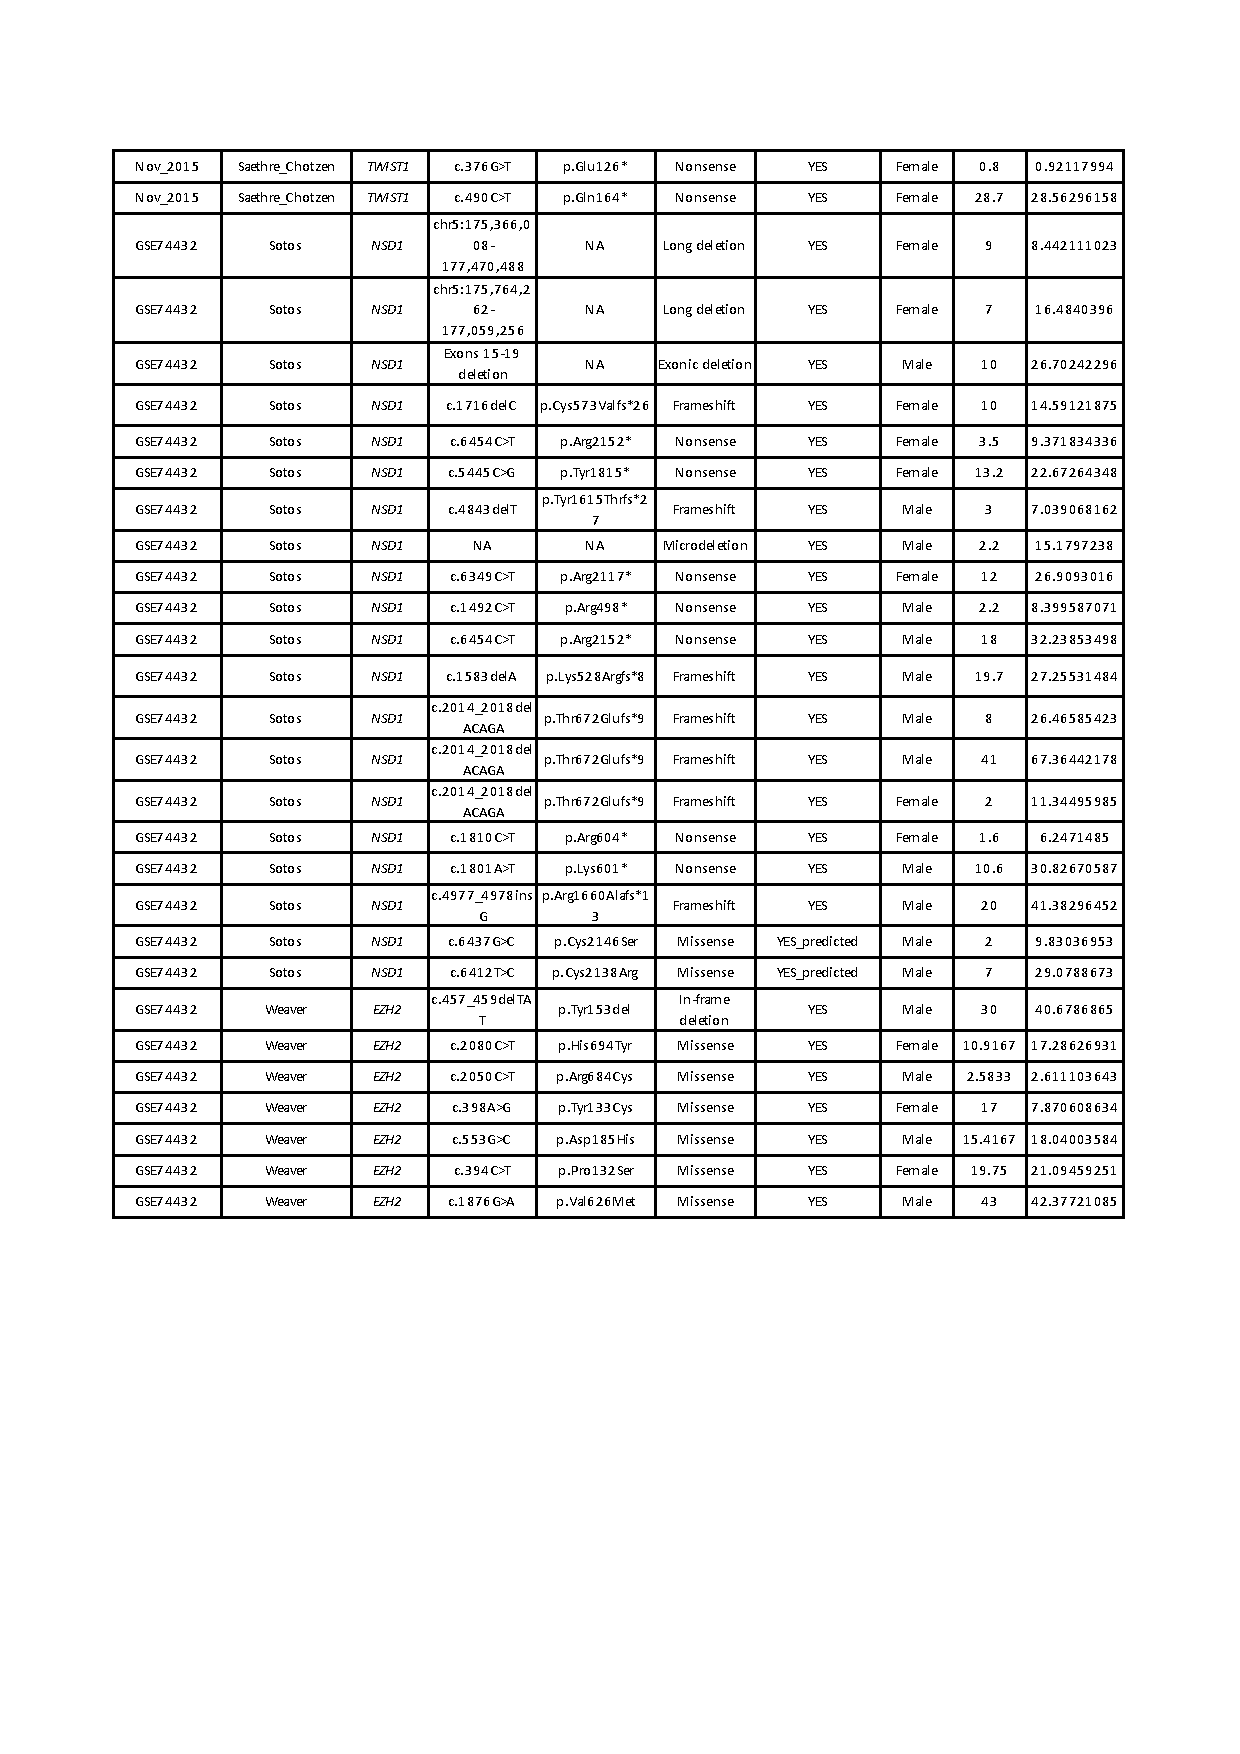
\includegraphics[width=1\textwidth]{SC3_Fig1_9}
	\caption[Table showing information for the individuals with developmental disorders]{Table showing information for the samples from individuals with developmental disorders (total $N=367$). Mutation information was annotated for the human genome assembly \textit{hg19}. \acrshort{ASD}: autism spectrum disorder; \acrshort{ATR-X}: alpha thalassemia/mental retardation X-linked syndrome; \acrshort{FXS}: fragile X syndrome.}
	\label{fig:sc3_fig1}
\end{figure}	

\begin{figure}[htbp!] 
	\centering    
	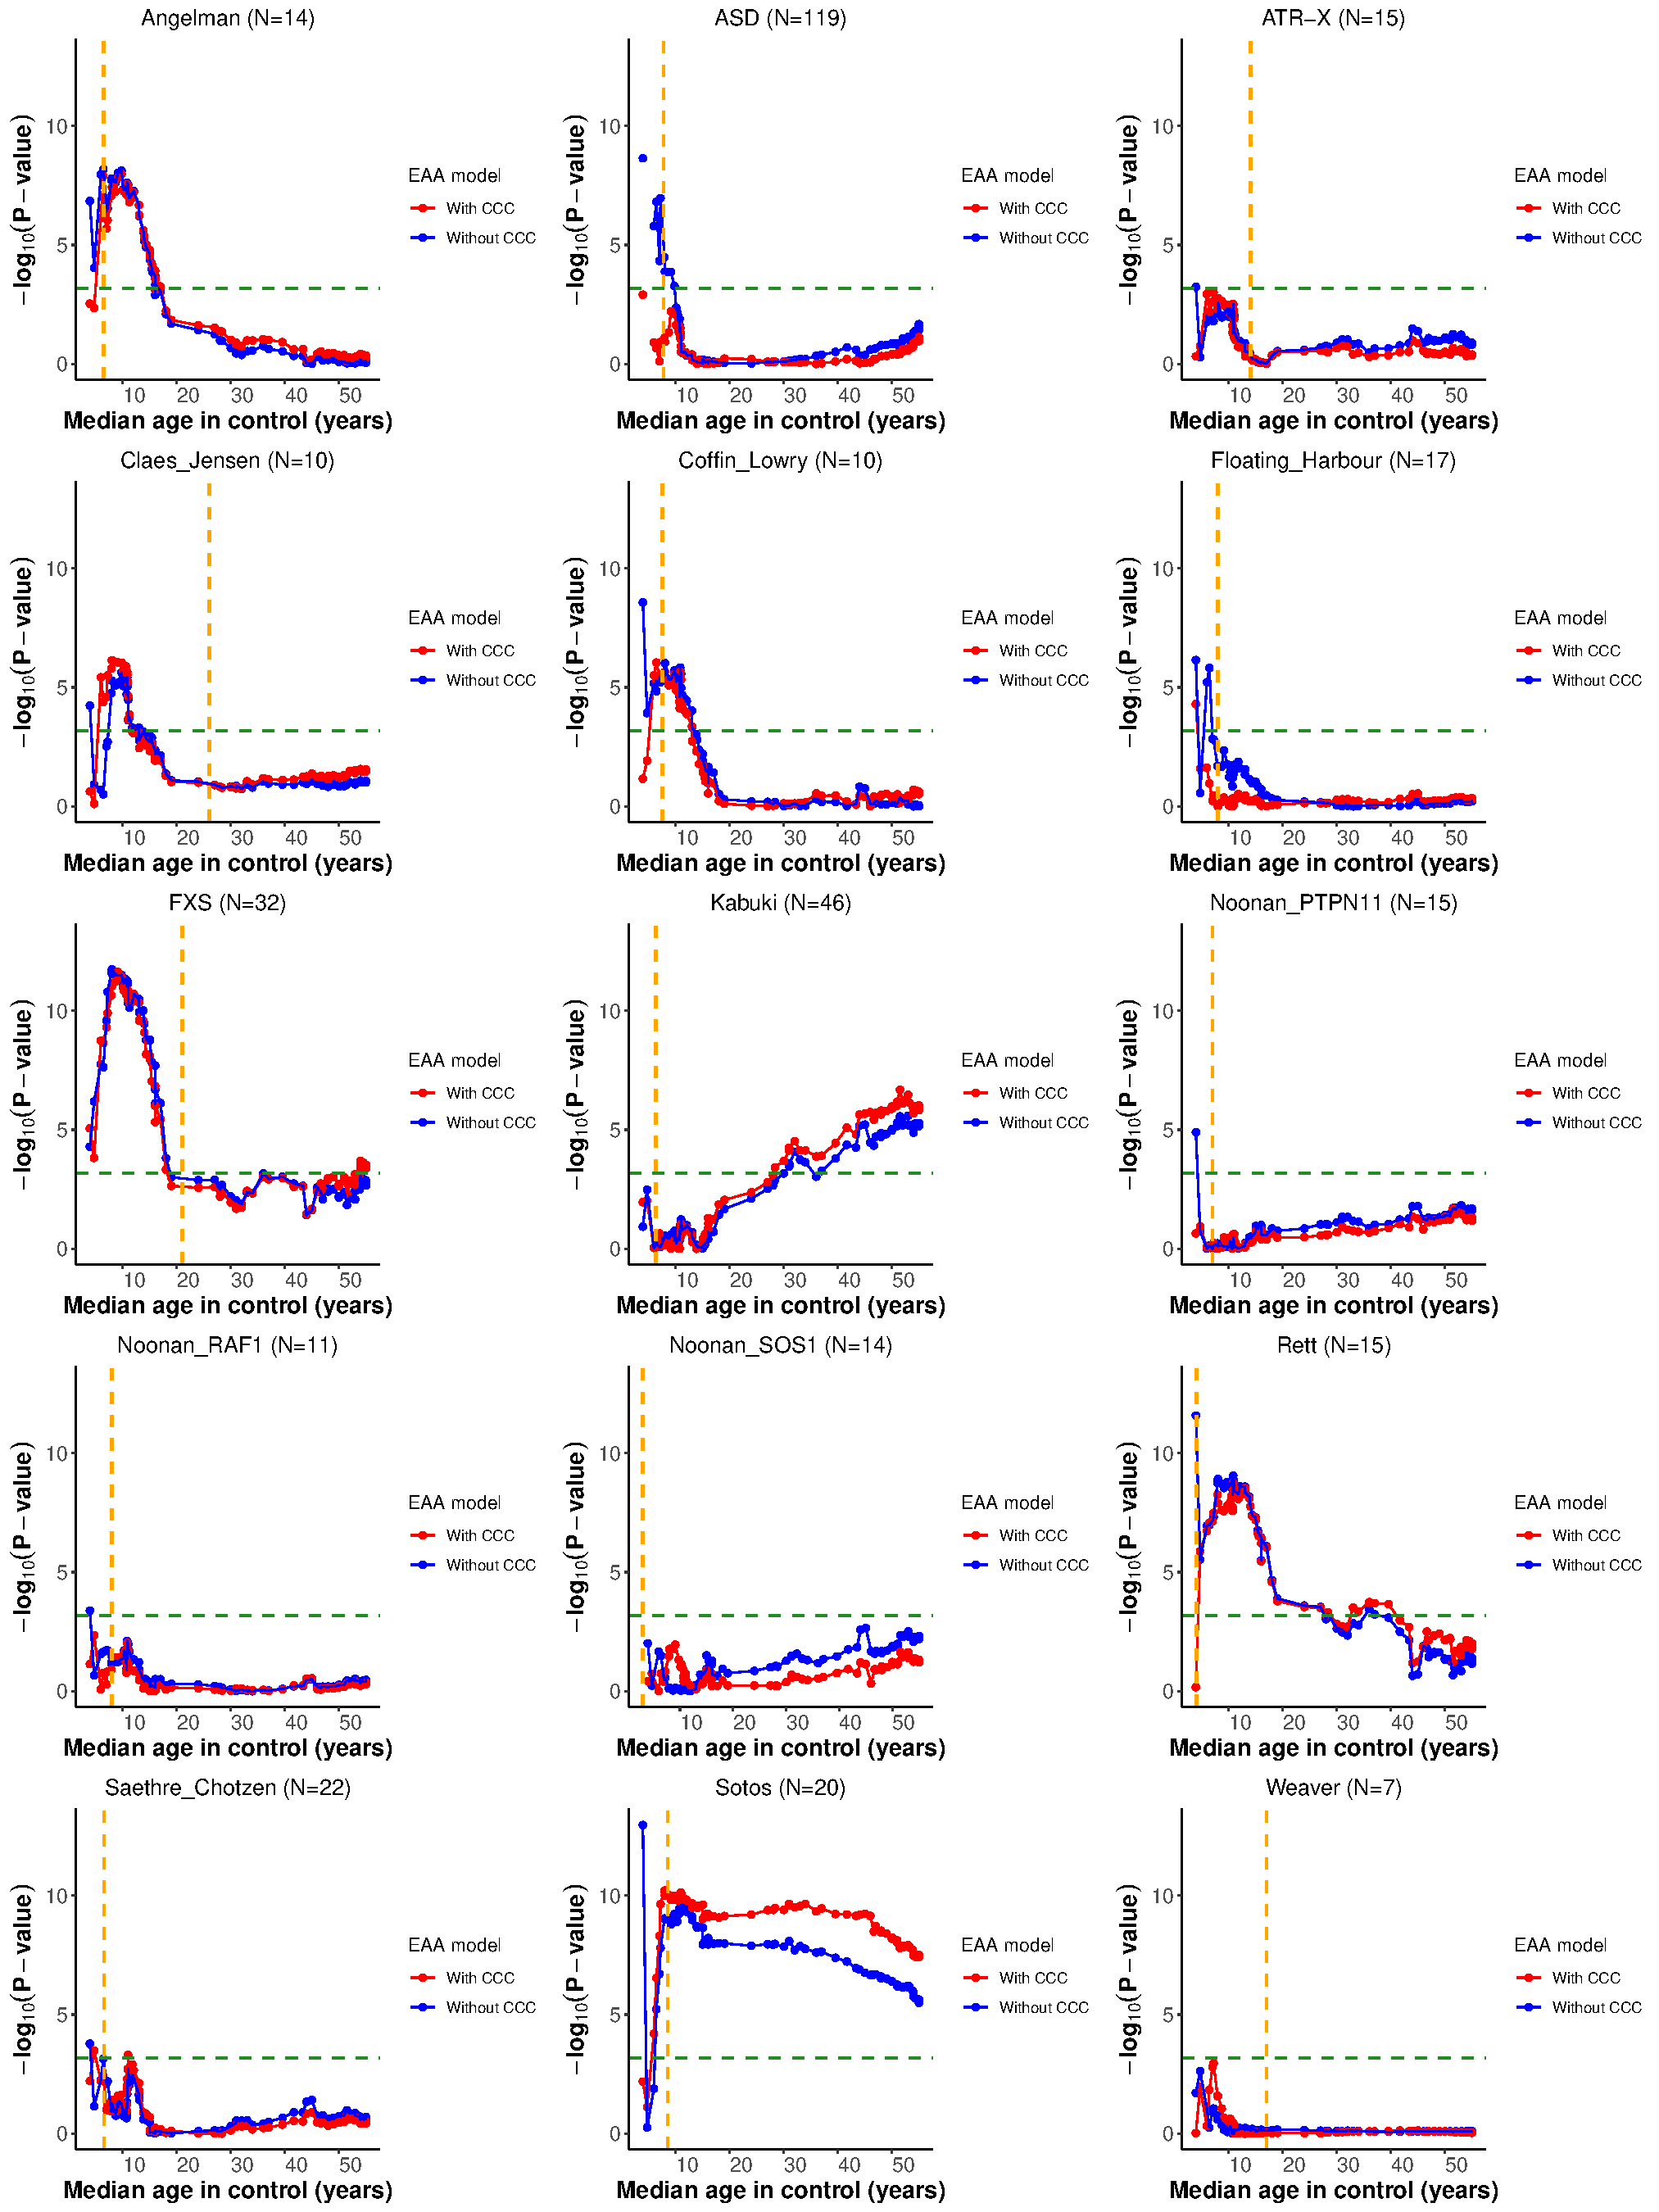
\includegraphics[width=1\textwidth]{SC3_Fig2}
	\caption[Effect of changing the median age of the controls when performing the screening]{Effect of changing the median age of the controls when performing the screening for epigenetic age acceleration (EAA) in the different developmental disorders. The dashed green line displays the significance level of $\alpha = 0.01$ after Bonferroni correction. The dashed orange line displays the median age for the samples in the developmental disorder considered. In blue: EAA model without cell composition correction (CCC). In red: EAA model with CCC. \acrshort{ASD}: autism spectrum disorder; \acrshort{ATR-X}: alpha thalassemia/mental retardation X-linked syndrome; \acrshort{FXS}: fragile X syndrome.}
	\label{fig:sc3_fig2}
\end{figure}

\begin{figure}[htbp!]
	\centering    
	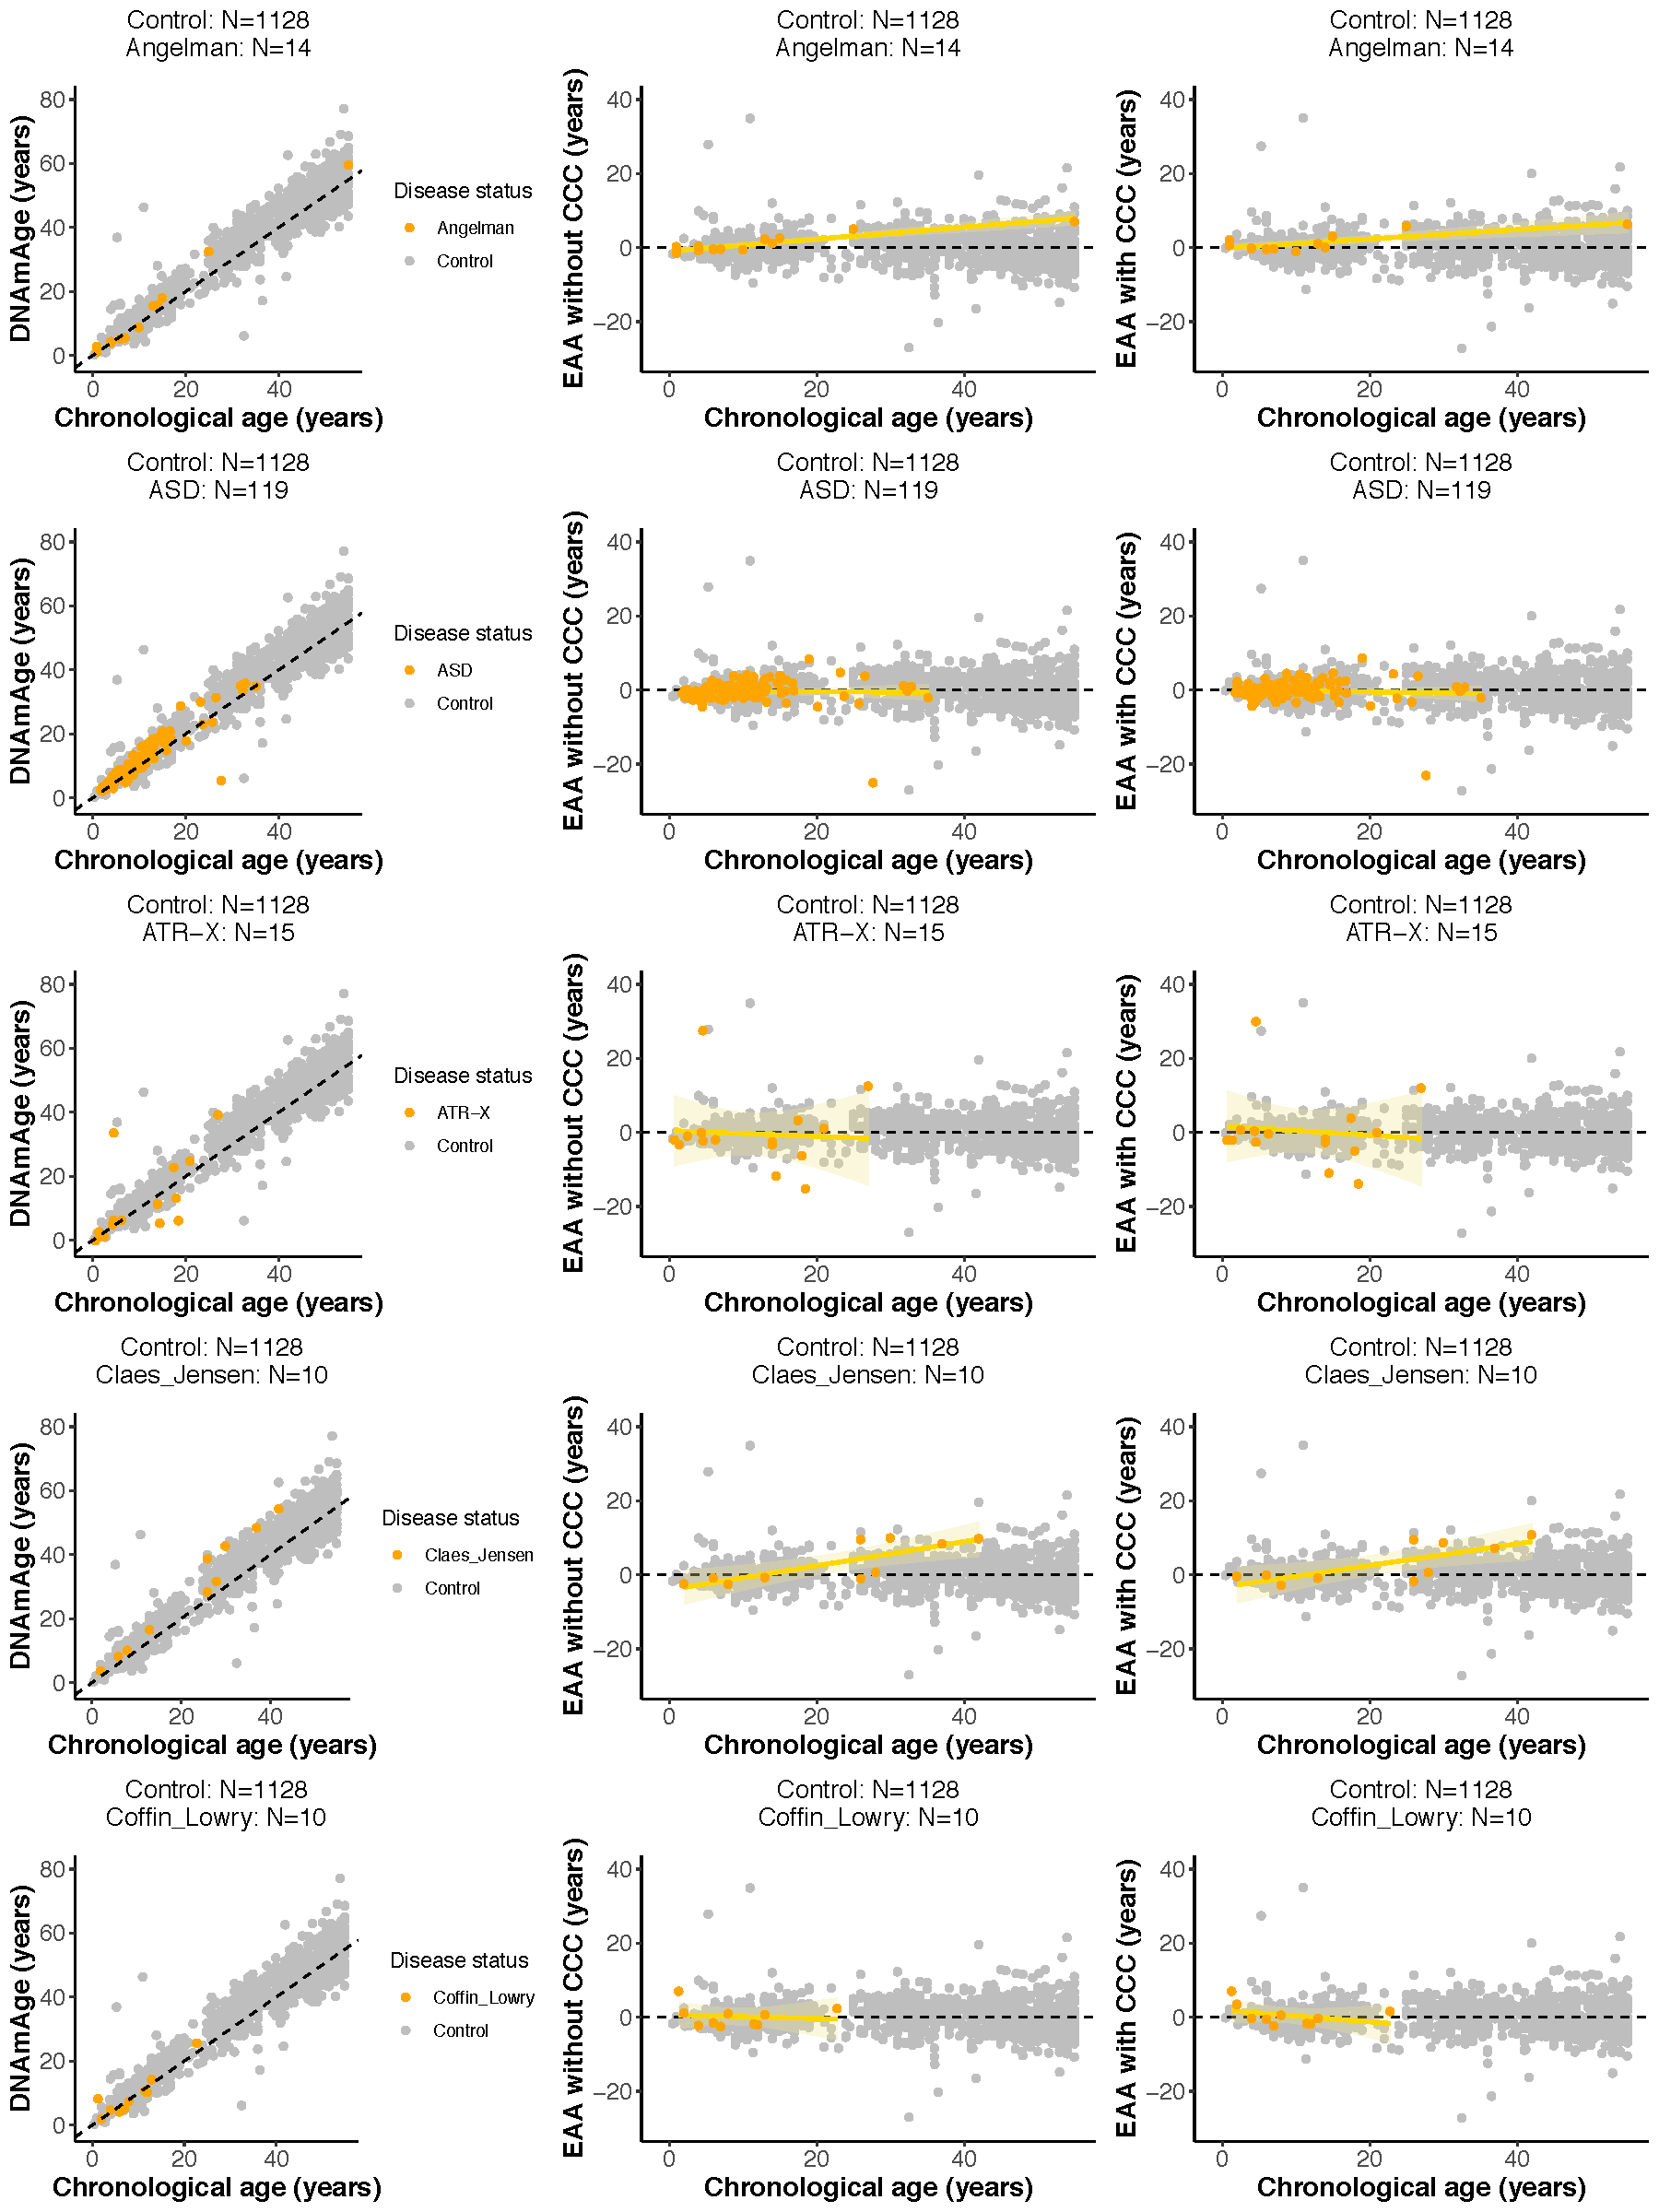
\includegraphics[width=1\textwidth]{SC3_Fig3_1}
\end{figure}
\begin{figure}[htbp!]
	\centering    
	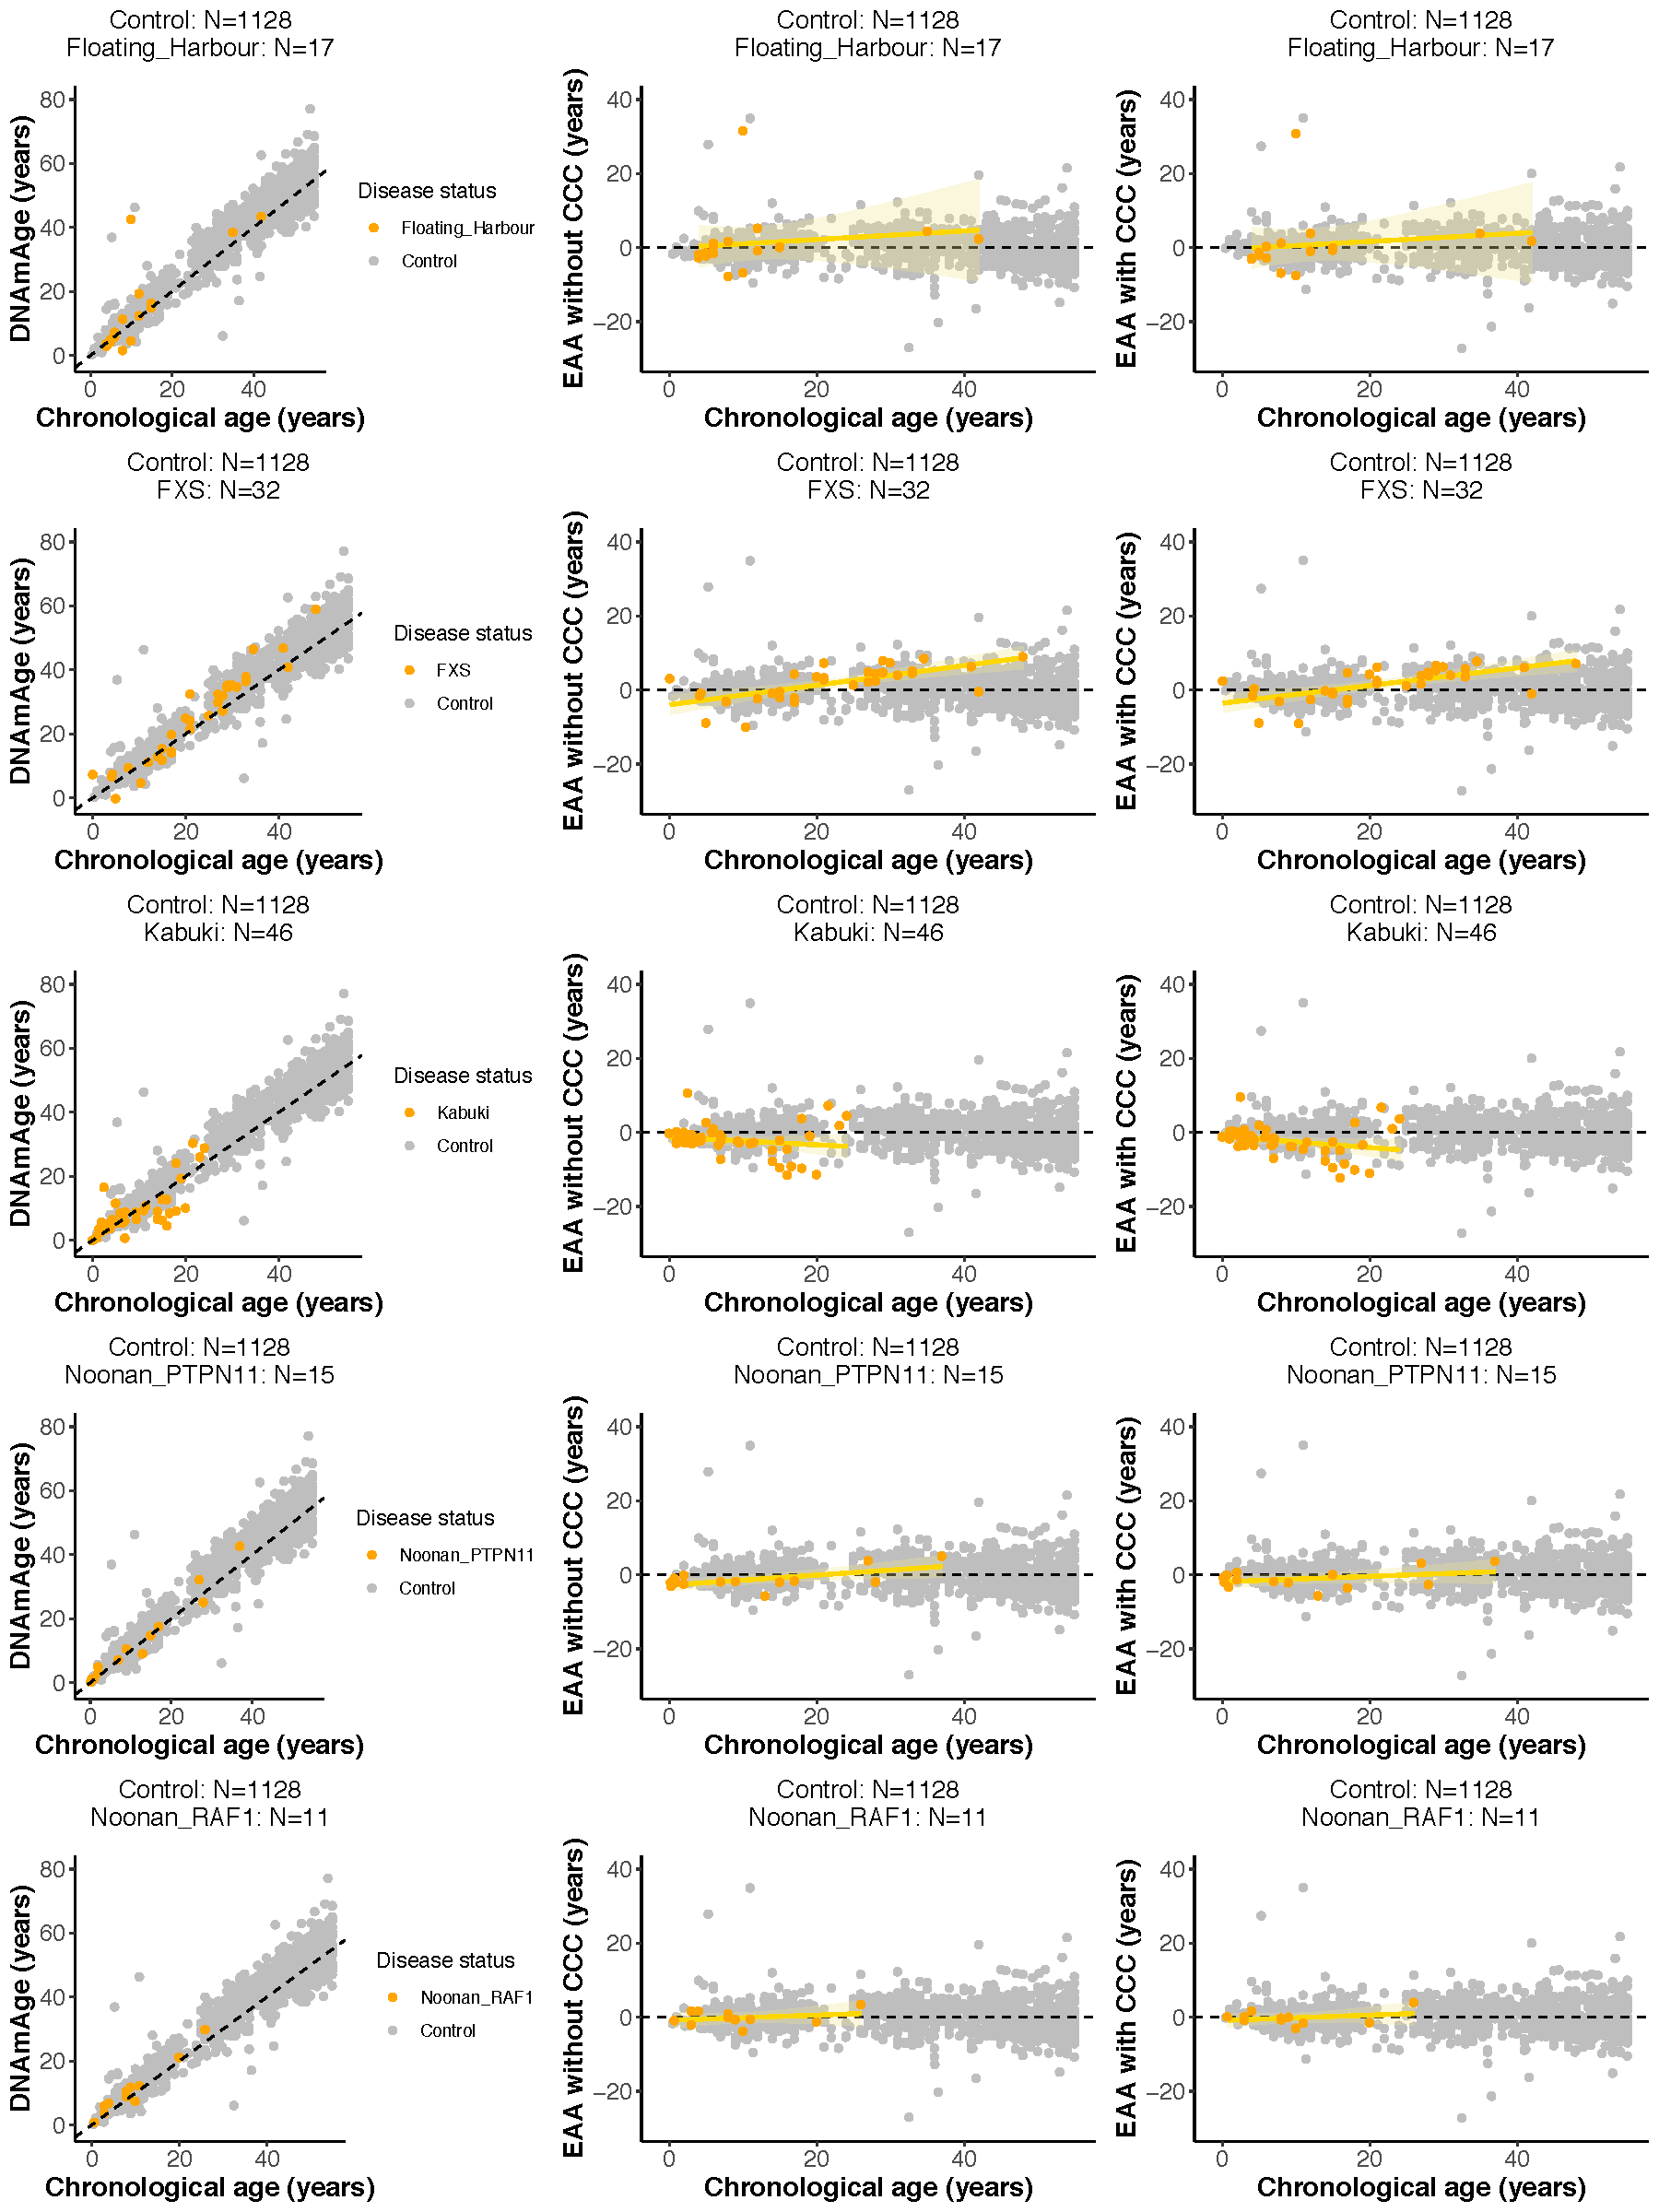
\includegraphics[width=1\textwidth]{SC3_Fig3_2}
\end{figure}
\begin{figure}[htbp!]
	\centering
	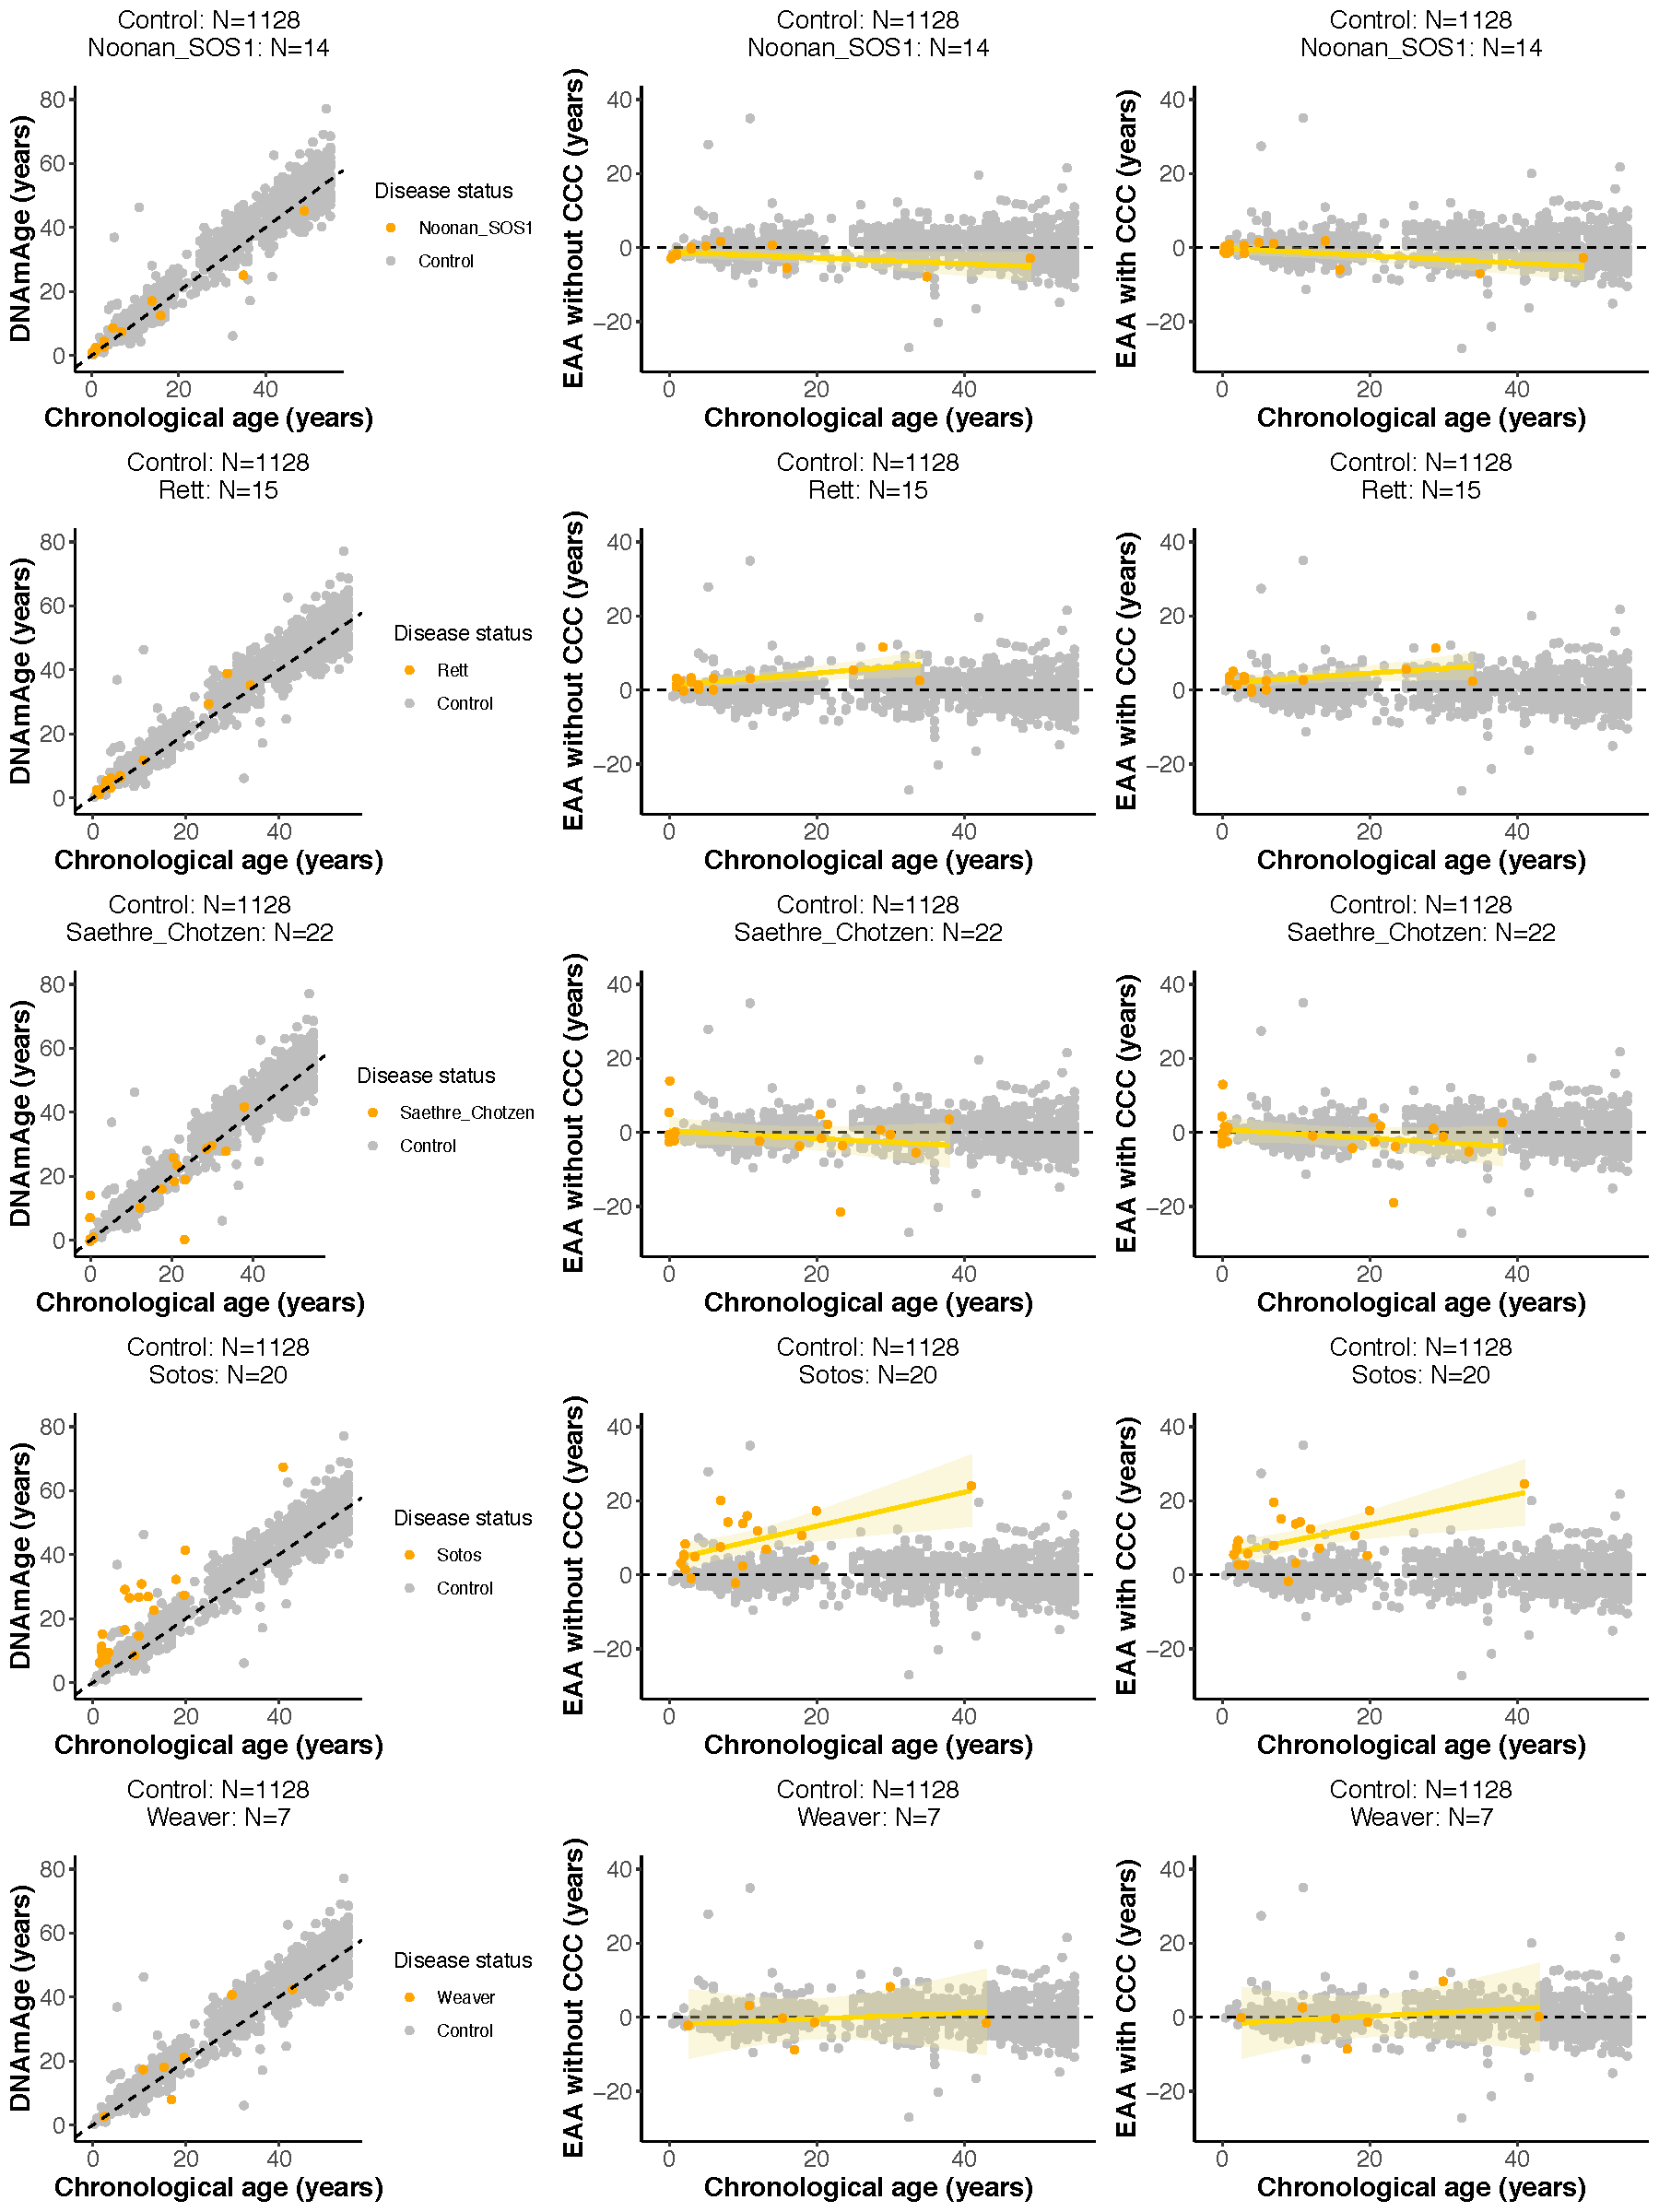
\includegraphics[width=1\textwidth]{SC3_Fig3_3}
	\caption[Screening for epigenetic age acceleration (EAA) in developmental disorders: additional scatterplots]{Screening for epigenetic age acceleration (EAA) in developmental disorders. Left panel: scatterplot showing the relation between epigenetic age ($DNAmAge$) according to Horvath’s model and chronological age of the samples for a given developmental disorder (orange) and control (grey). Each sample is represented by one point. The black dashed line represents the diagonal to aid visualisation. Middle and right panels: scatterplots showing the relation between the epigenetic age acceleration (EAA) (without and with CCC respectively) and chronological age of the samples for a given developmental disorder (orange) and control (grey). Each sample is represented by one point. The yellow line represents the linear model EAA $\sim$ Age, with the standard error shown in the light yellow shade.}
	\label{fig:sc3_fig3}
\end{figure}

\begin{figure}[htbp!] 
	\centering    
	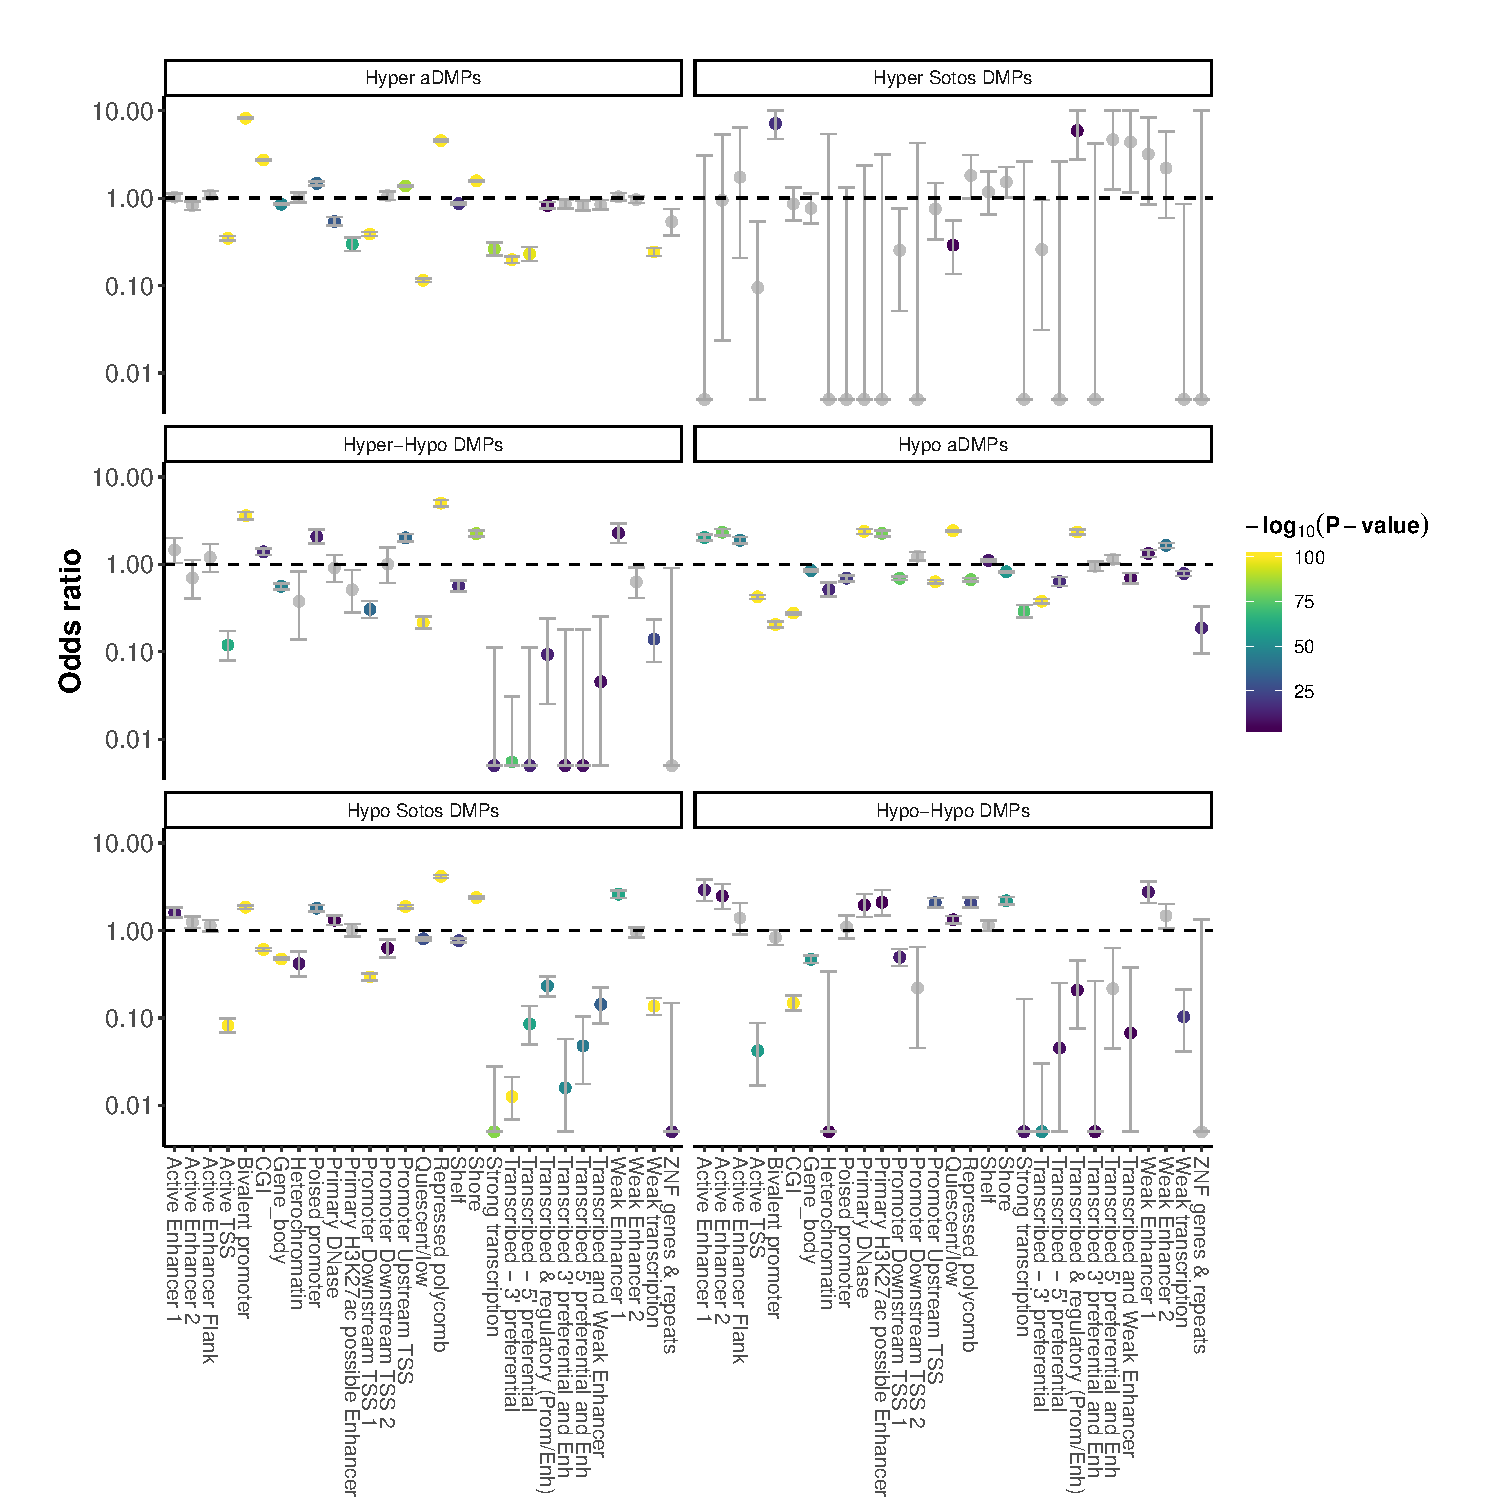
\includegraphics[width=1.1\textwidth]{SC3_Fig4}
	\vspace*{2 mm}
	\caption[Enrichment for the categorical (epi)genomic features in Sotos and ageing: genome-wide]{Enrichment for the categorical (epi)genomic features considered when comparing the different genome-wide subsets of differentially methylated positions (DMPs) in ageing and Sotos against a control (see section~\ref{s:3.7}). The y-axis represents the odds ratio (OR), the error bars show the 95\% confidence interval for the OR estimate and the colour of the points codes for $-\log_{10}(\text{p-value})$ obtained after testing for enrichment using Fisher's exact test. An OR > 1 shows that the given feature is enriched in the subset of DMPs considered, whilst an OR < 1 shows that it is found less than expected. The `Hyper-Hypo DMPs' subset results from the intersection between the hypermethylated DMPs in ageing and the hypomethylated DMPs in Sotos. The `Hypo-Hypo DMPs' subset results from the intersection between the hypomethylated DMPs in ageing and Sotos. In grey: features that did not reach significance using a significance level of $\alpha = 0.01$ after Bonferroni correction.}
	\label{fig:sc3_fig4}
\end{figure}

\begin{figure}[htbp!] 
	\centering    
	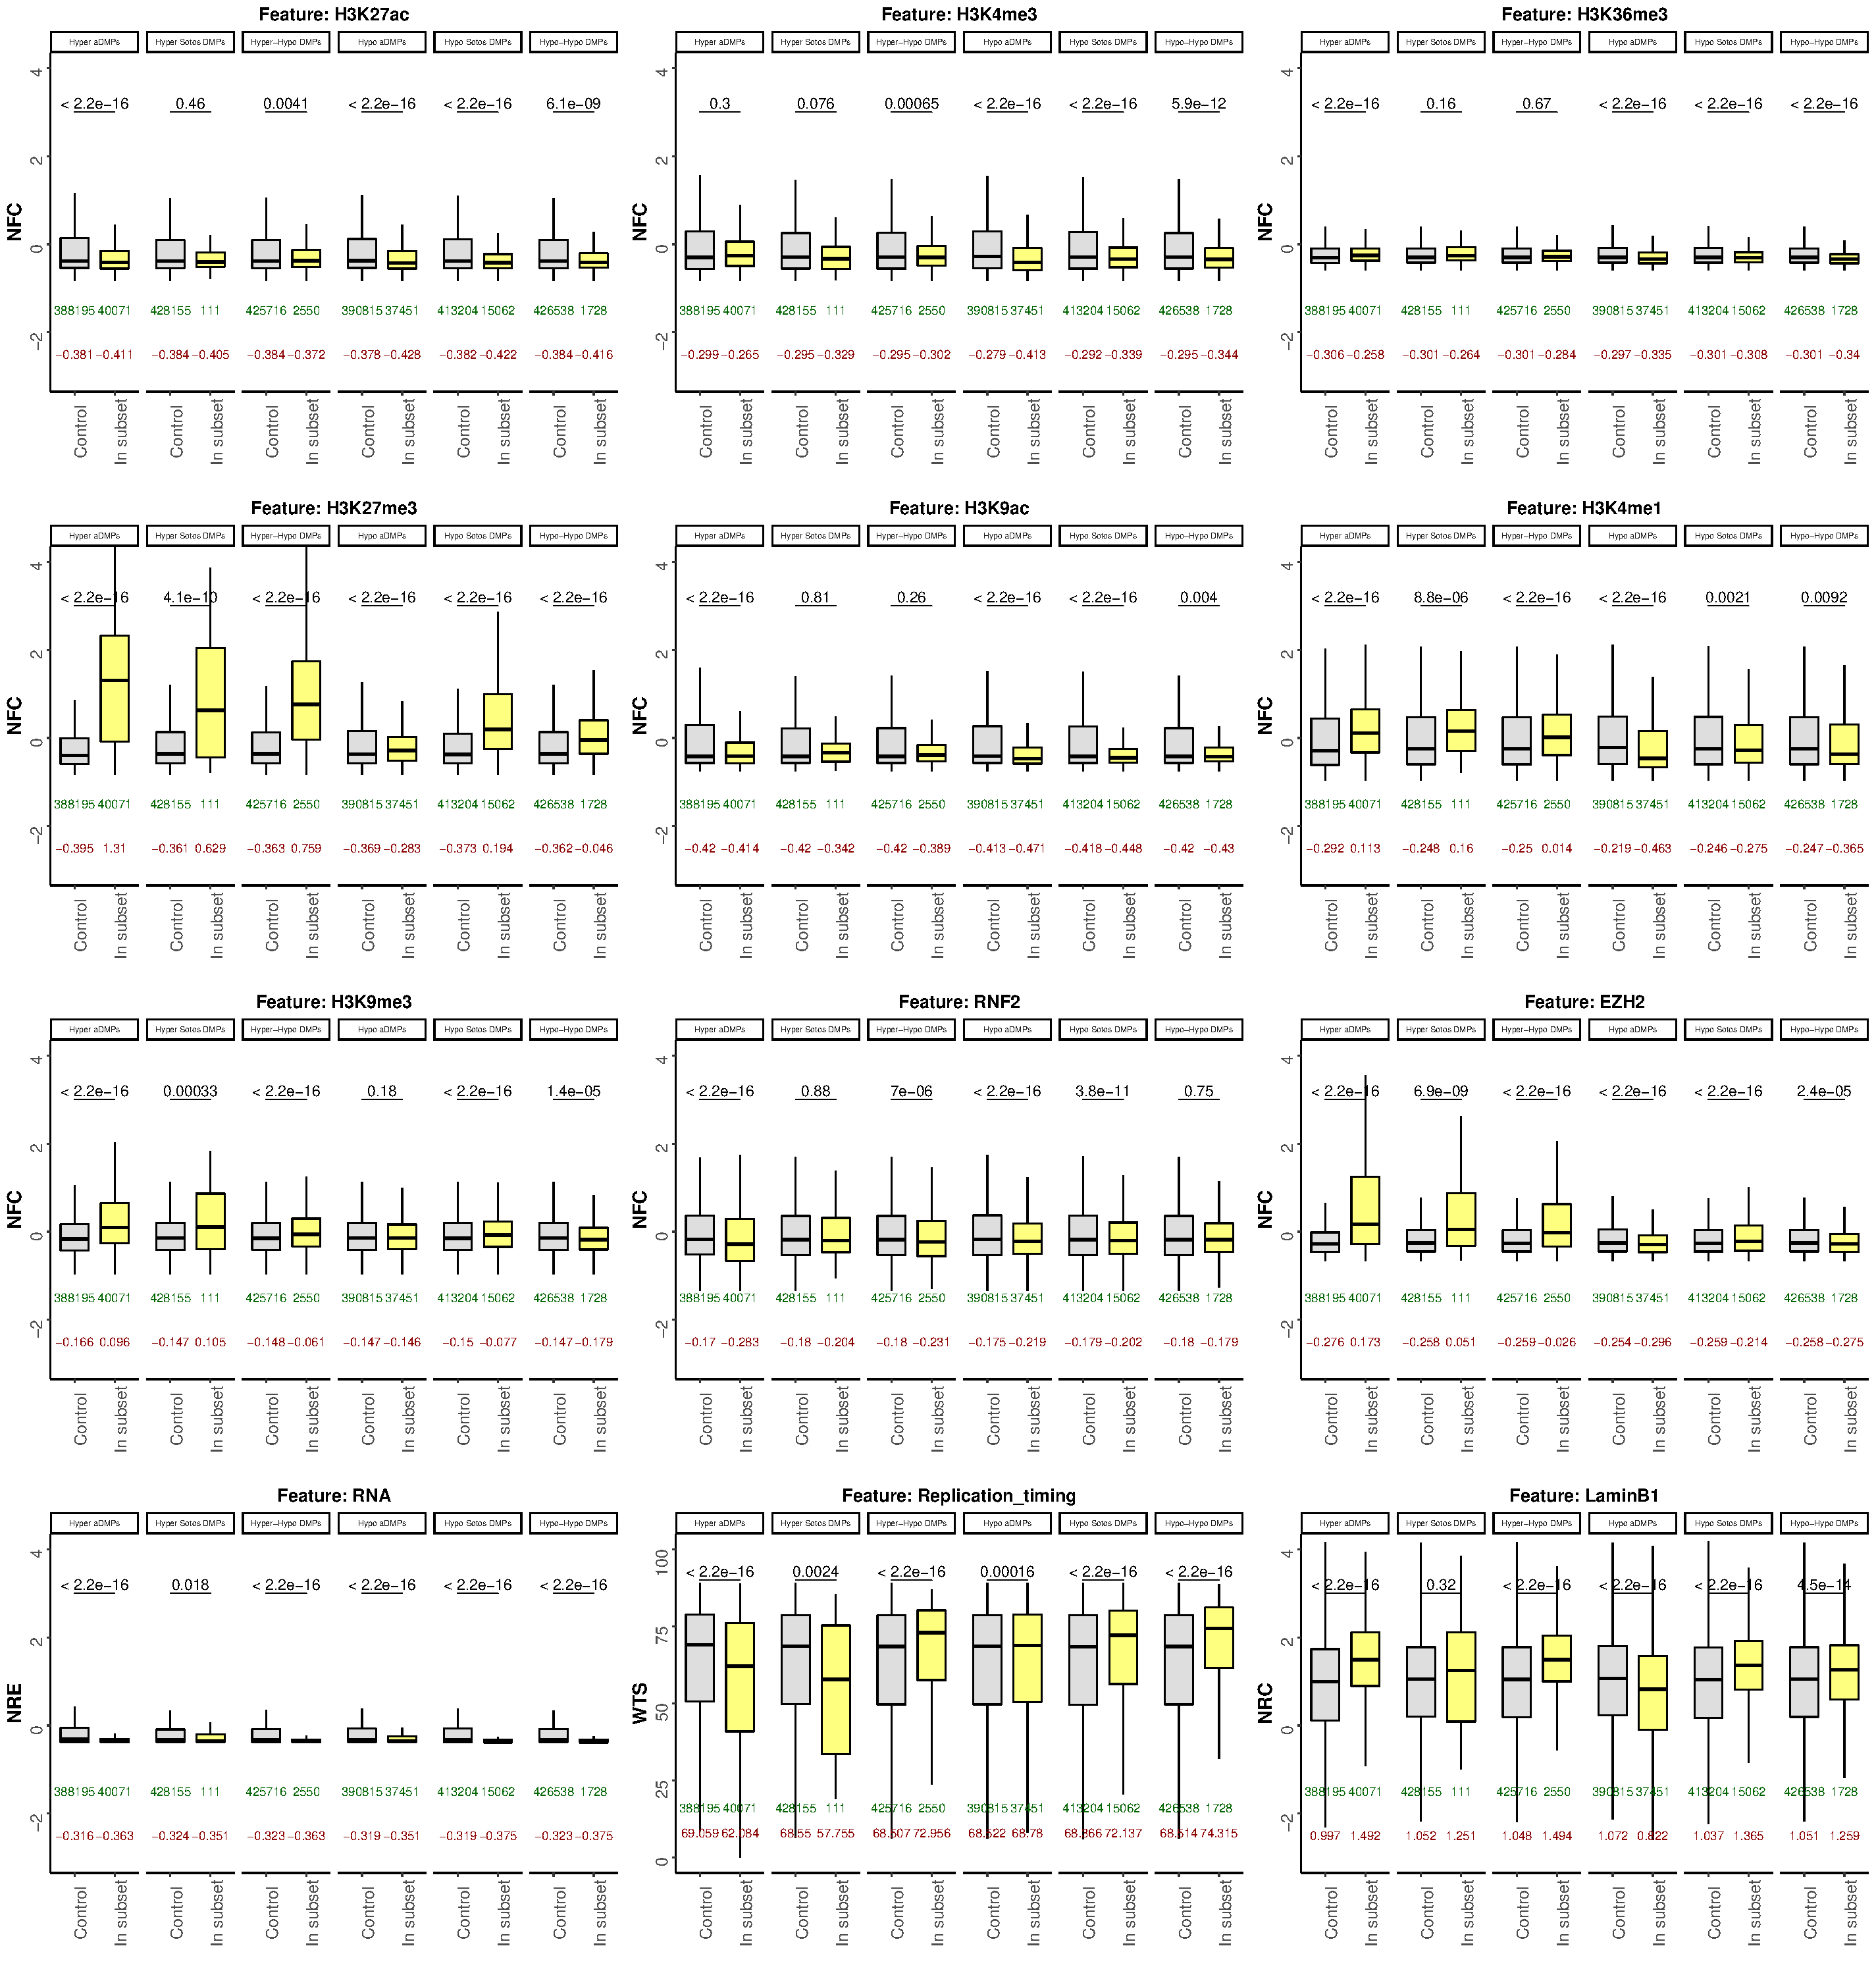
\includegraphics[width=1\textwidth]{SC3_Fig5}
	\caption[Distributions of scores for the continuous (epi)genomic features in Sotos and ageing: genome-wide]{Boxplots showing the distributions of scores for the continuous (epi)genomic features considered when comparing the different genome-wide subsets of differentially methylated positions (DMPs) in ageing and Sotos against a control (see section~\ref{s:3.7}). The p-values (two-sided Wilcoxon's test, before multiple testing correction) are shown above the boxplots. The number of DMPs belonging to each subset (in green) and the median value of the feature score (in dark red) are shown below the boxplots. \acrshort{NFC}: `normalised fold change'; \acrshort{NRE}: `normalised RNA expression'; \acrshort{WTS}: `wavelet-transformed signals'; \acrshort{NRC}: `normalised read counts'.}
	\label{fig:sc3_fig5}
\end{figure}

\begin{figure}[htbp!] 
	\centering    
	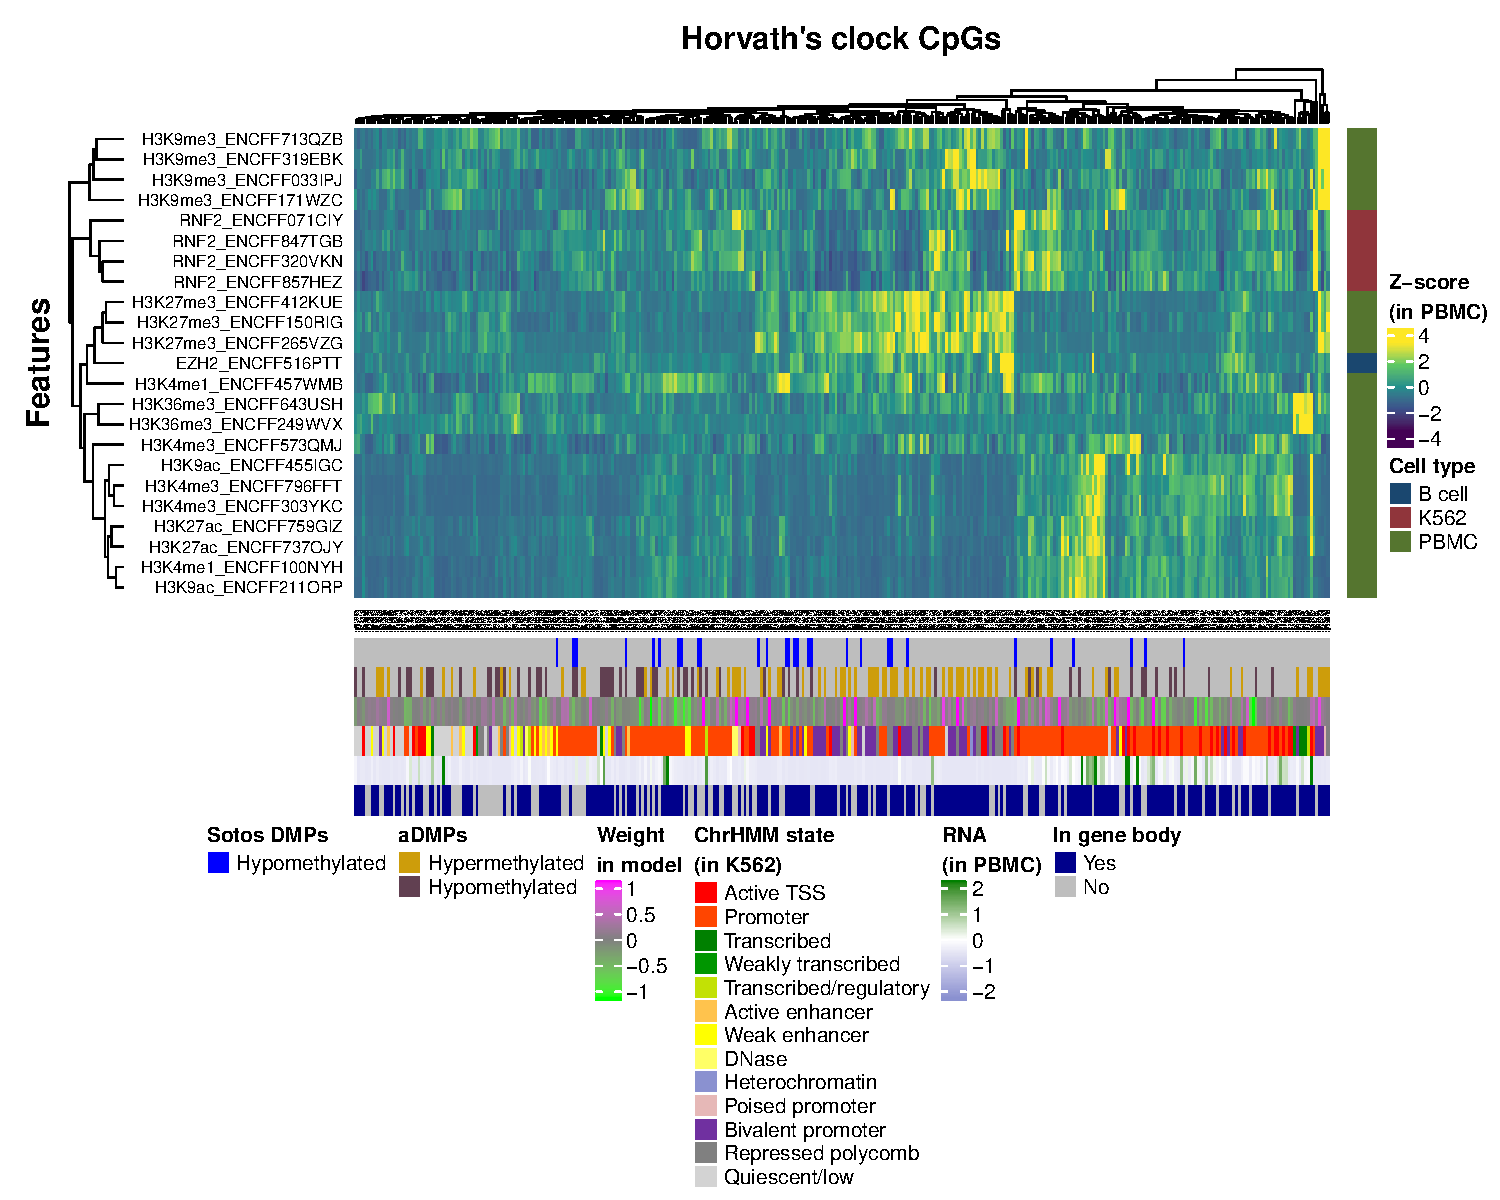
\includegraphics[width=1\textwidth]{SC3_Fig6}
	\vspace*{1 mm}
	\caption[Scores for the continuous (epi)genomic features in the Horvath's epigenetic clock CpGs]{Heatmap displaying the scores for the different continuous (epi)genomic features (rows) in each one of the 353 Horvath's epigenetic clock CpGs (columns). The names of the features include the ENCODE ID (see Fig.~\ref{fig:sc3_figadd}). Hierarchical clustering was performed in both rows and columns. RNA refers to the `normalised RNA expression' (NRE). aDMPs: differentially methylated positions during ageing. PBMC: peripheral blood mononuclear cells.}
	\label{fig:sc3_fig6}
\end{figure}

\begin{figure}[htbp!] 
	\centering    
	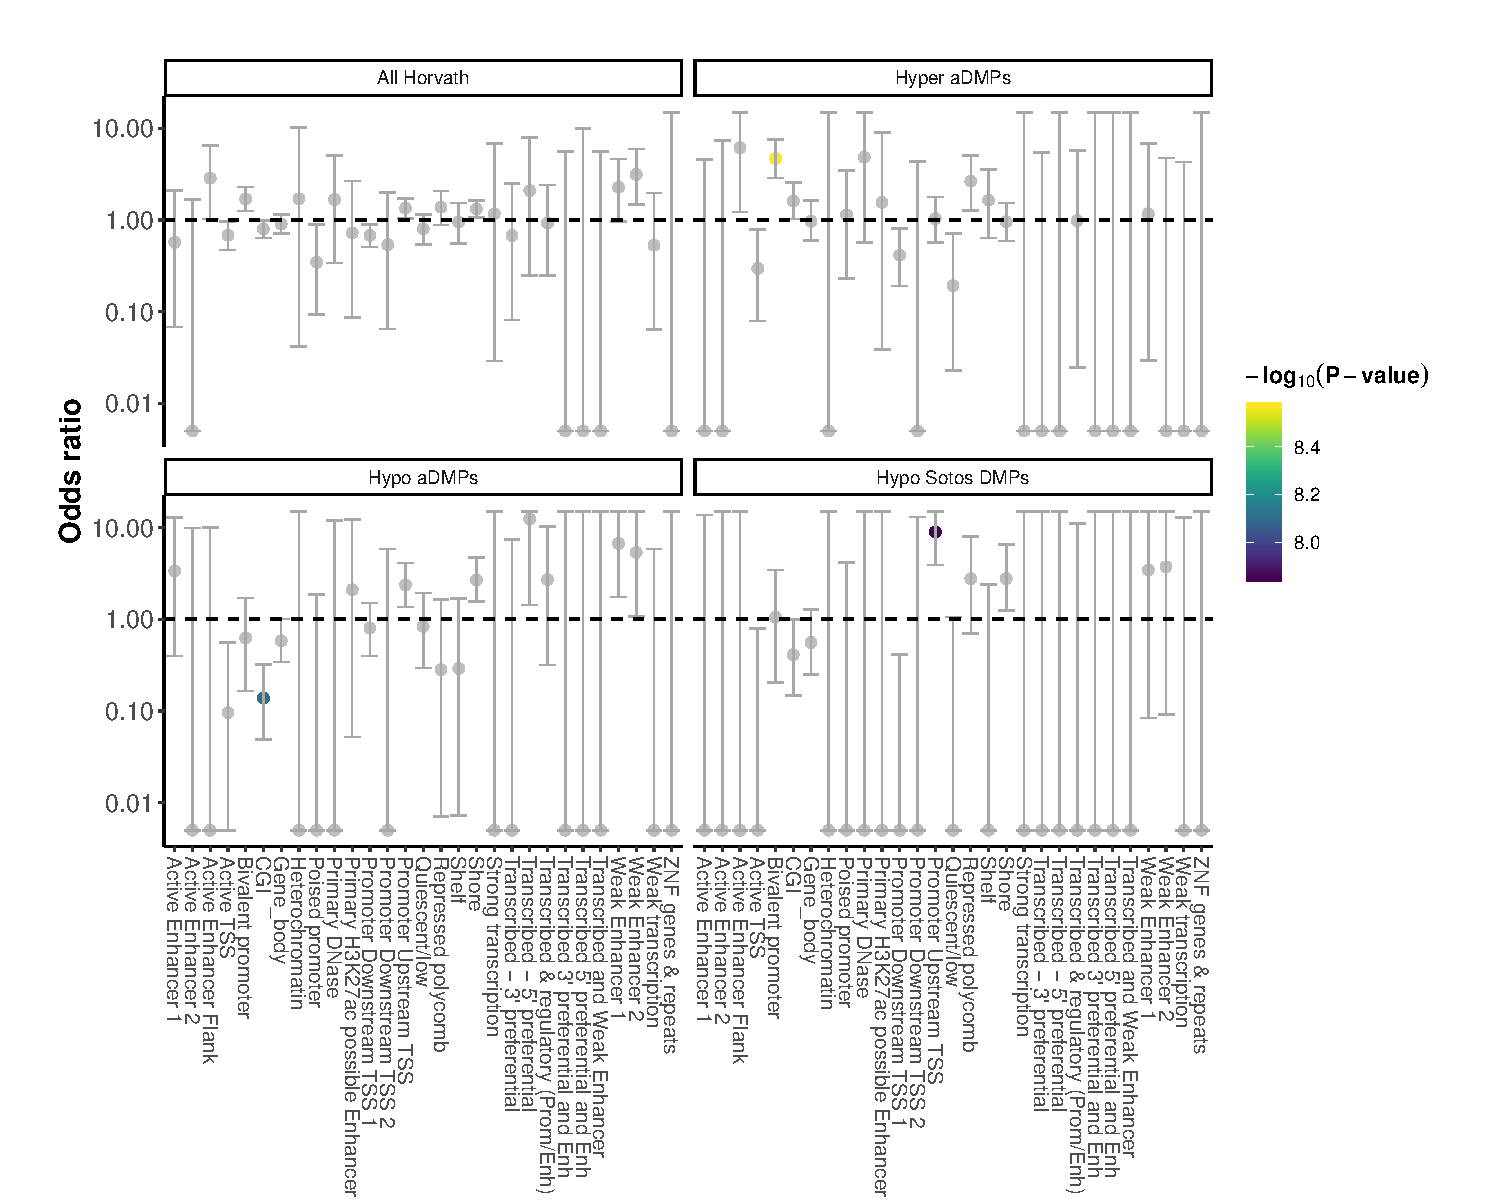
\includegraphics[width=1\textwidth]{SC3_Fig7}
	\caption[Enrichment for the categorical (epi)genomic features in Sotos and ageing: Horvath's epigenetic clock]{As in Fig.~\ref{fig:sc3_fig4}., but focused on the 353 Horvath's epigenetic clock CpG sites.}
	\label{fig:sc3_fig7}
\end{figure}

\begin{figure}[htbp!] 
	\centering    
	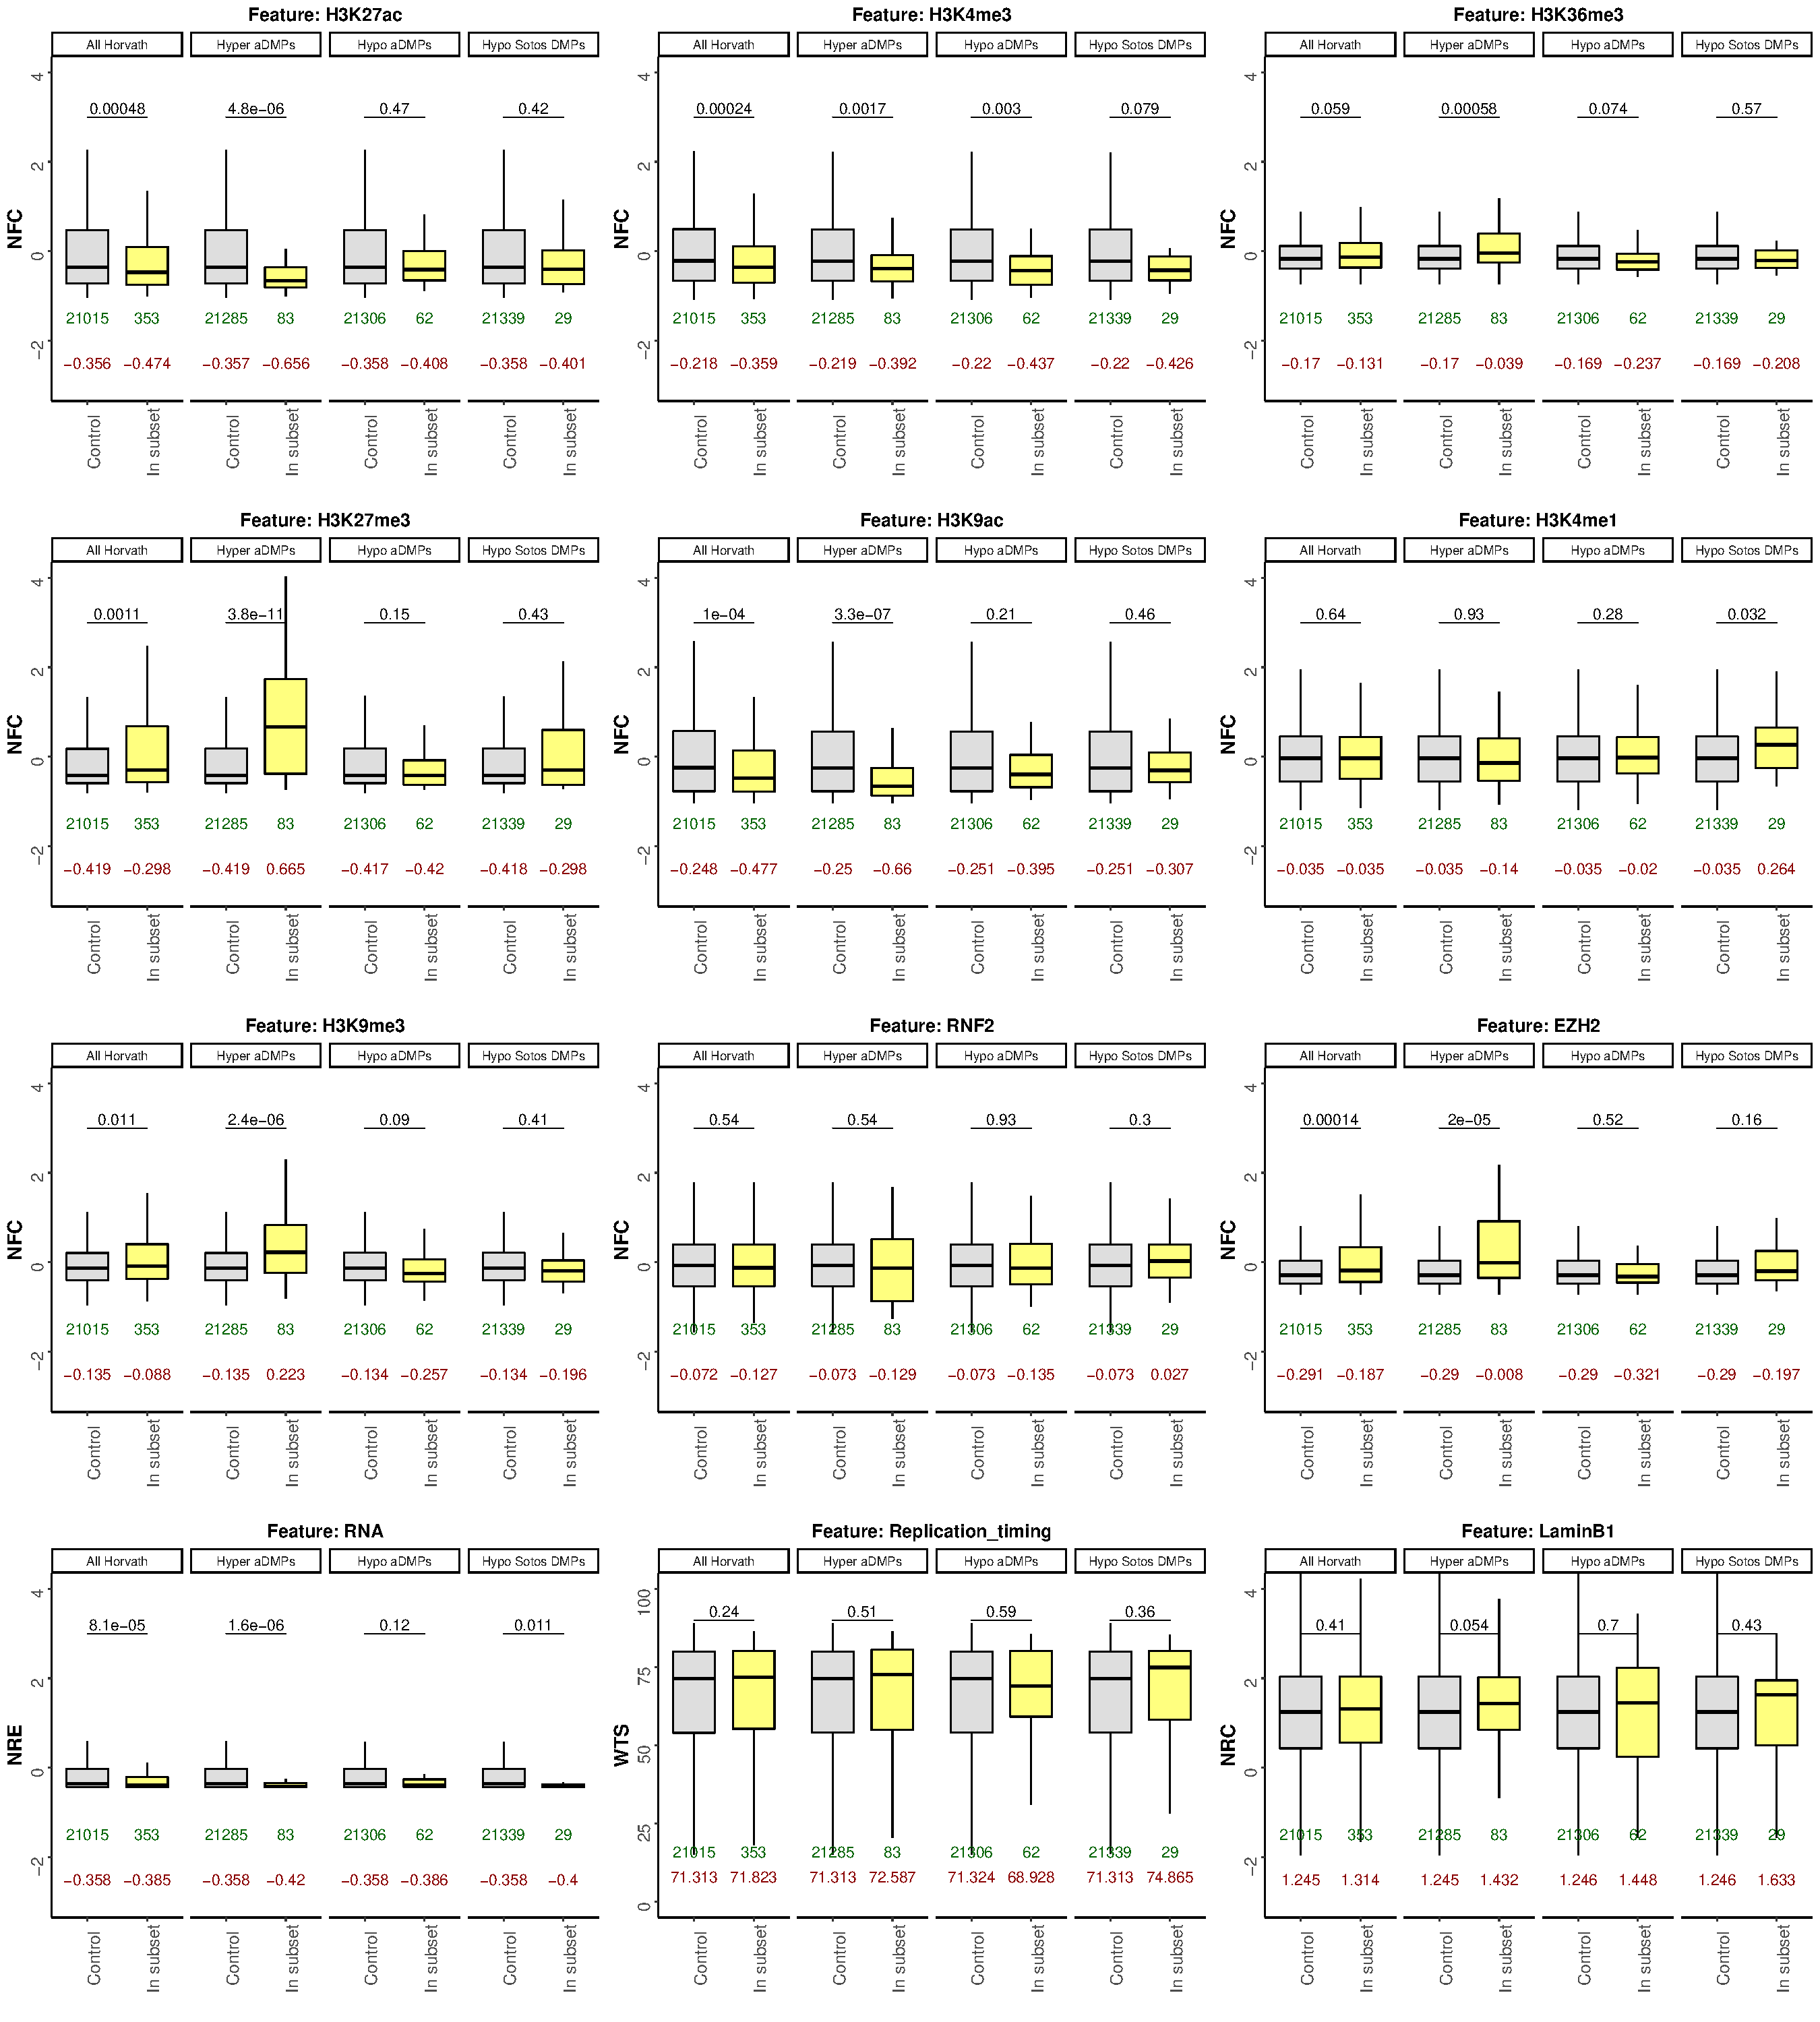
\includegraphics[width=1\textwidth]{SC3_Fig8}
	\caption[Distributions of scores for the continuous (epi)genomic features in Sotos and ageing: Horvath's epigenetic clock]{As in Fig.~\ref{fig:sc3_fig5}., but focused on the 353 Horvath's epigenetic clock CpG sites.}
	\label{fig:sc3_fig8}
\end{figure}

\begin{figure}[htbp!] 
	\centering    
	\includegraphics[width=1\textwidth]{SC3_Fig9}
	\caption[Methylation Shannon entropy acceleration]{Methylation Shannon entropy acceleration. \textbf{a.} Scatterplot showing the relationship between the genome-wide Shannon entropy acceleration (\acrshort{gSEA}) and chronological age of the samples for Sotos (orange) and healthy controls (grey). Each sample is represented by one point. The yellow line represents the linear model gSEA $\sim$ Age, with the standard error shown in the light yellow shade. \textbf{b.} As in a., but using the Shannon entropy acceleration calculated only for the 353 CpG sites in the Horvath's epigenetic clock (\acrshort{cSEA}).}
	\label{fig:sc3_fig9}
\end{figure}

\begin{figure}[htbp!] 
	\centering    
	\includegraphics[width=0.5\textwidth]{SC3_Fig10}
	\caption[Batch effects in the methylation Shannon entropy for the epigenetic clock sites]{Scatterplot showing the effects of the different batches on the methylation Shannon entropy calculations for the 353 Horvath's epigenetic clock sites. Each sample is represented by one point and coloured according to the batch that they belong to. }
	\label{fig:sc3_fig10}
\end{figure}

		

\begin{figure}[htbp!] 
	\centering    
	\includegraphics[width=1\textwidth]{SC3_Figadd}
	\caption[Information for the continuous (epi)genomic features]{Information (including the source) about the continuous (epi)genomic features (\acrshort{ChIP-seq} and \acrshort{RNA-seq} data) that were included in my analysis to annotate the different sets of CpG sites. All the data were mapped to the \textit{\acrshort{hg19}} assembly of the human genome. \acrshort{PBMC}: peripheral blood mononuclear cells.}
	\label{fig:sc3_figadd}
\end{figure}

\clearpage

\renewcommand{\thesection}{S.3}   
\section{Technological aspects of epigenetic clocks}

\renewcommand\thefigure{S3.\arabic{figure}}    
\bigskip

\begin{figure}[htbp!] 
	\centering    
	\setcounter{figure}{0}
	\includegraphics[width=0.7\textwidth]{SC4_Fig1}
	\caption[Scatterplot of fragment length distributions for the isoschizomer families]{Scatterplot which summarises the fragment length distributions for the same isoschizomer families portrayed in Fig~\ref{fig:c4_fig2}a. The red dots represent the actual values of median fragment length and total number of fragments for each family. The black lines assign each name label to the correspondent red point for visualization purposes.}
	\label{fig:sc4_fig1}
\end{figure}

\begin{figure}[htbp!] 
	\centering    
	\includegraphics[width=1\textwidth]{SC4_Fig2}
	\caption[Genomic features that overlap with restriction enzyme cleavage sites]{Matrix of scatterplots showing the percentages of cleavage sites from different restriction enzymes that overlap with several genomic features (listed on the diagonal) in the human genome (hg38). The red dot in each scatterplot represents the values for MspI. The numbers above the diagonal are the Pearson correlation coefficients between all the possible pairs of genomic features.}
	\label{fig:sc4_fig2}
\end{figure}

\begin{figure}[htbp!] 
	\centering    
	\includegraphics[width=1.0\textwidth]{SC4_Fig3}
	\caption[Comparison of studies using restriction enzymes for genomic enrichment]{Table showing the comparison of different studies that have attempted to use restriction enzymes to target different regions in the genome.}
	\label{fig:sc4_fig3}
\end{figure}

\begin{figure}[htbp!] 
	\centering    
	\includegraphics[width=1.0\textwidth]{SC4_Fig4}
	\vspace*{1mm}
	\caption[Additional insights into cuRRBS]{Additional insights into cuRRBS. \textbf{a.} Detailed flowchart showing the input, main steps in cuRRBS and the output of the software. \textbf{b.} Violin plots showing the distribution of Pearson's correlation coefficients between the number of fragments (\textit{NF}) and the \textit{Score} for all the different enzymes tested with cuRRBS (single-enzyme, double-enzyme, all). In this example we used the Horvath epigenetic clock system \cite{Horvath2013}, checking all the \textit{size ranges} between 20 and 1000 bp, with an \textit{experimental error} of 10 bp and a \textit{read length} of 75 bp. Each yellow point represents the median for the Pearson's correlation coefficients under consideration. \textbf{c.} Density plot showing the distribution of the \textit{robustness} (\textit{R}) values when assuming an \textit{experimental error} ($\delta$) of 20 bp. cuRRBS was run for all the biological systems under study (Fig.~\ref{fig:sc4_fig5}) \cite{Horvath2013,Hanna2016,Milagre2017,Kawakatsu2016,Maurano2015,LevMaor2015,Domcke2015} with the same parameters as described in `Running cuRRBS for different \textit{in silico} systems' in section~\ref{s:4.7} (all the hits that satisfied the \textit{thresholds} were reported in this case). The dashed blue line represents the median (0.9734). The different colours provide a way to judge the \textit{robustness} values: bad (in red, $R < Q_1 = 0.9580$), medium (in orange, $Q_1 \leq R \leq Q_3 = 0.9834$) and good (in green, $R > Q_3$); where $Q_1$ and $Q_3$ represent the first and the third quartiles respectively.}
	\label{fig:sc4_fig4}
\end{figure}

\begin{figure}[htbp!] 
	\centering    
	\includegraphics[width=1.0\textwidth]{SC4_Fig5}
	\caption[Additional results of running cuRRBS in different biological systems]{Table showing the information regarding the different biological systems \cite{Horvath2013,Hanna2016,Milagre2017,Kawakatsu2016,Maurano2015,LevMaor2015,Domcke2015} for which cuRRBS was run \textit{in silico}. Some variables from the top hits in cuRRBS output are also reported.}
	\label{fig:sc4_fig5}
\end{figure}

\begin{figure}[htbp!] 
	\centering    
	\includegraphics[width=1.0\textwidth]{SC4_Fig6}
	\vspace*{2mm}
	\caption[Effect of experimental errors during size selection in cuRRBS predictions]{Effect of experimental errors during size selection in cuRRBS predictions. \textbf{a.} Barplots showing the difference in the number of true positives (TP, in green), true negatives (TN, in blue), false positives (FP, in red) and false negatives (FN, in yellow) derived from cuRRBS theoretical predictions for the XmaI-RRBS data \cite{Tanas2017} using two different size ranges: 110-200 bp (aimed size range) and 90-185 bp (real size range). The difference observed between the two size ranges (aimed - real) is expressed as the percentage of the total number of sites considered (i.e. all CGI- CpGs). The number of sites in each category is calculated for different thresholds in the depth of coverage (number of reads covering a CpG site as reported by Bismark). cuRRBS was run for XmaI with all the default parameters (with a \textit{read length} of 200 bp). Legend is displayed on the right hand side. \textbf{b.} Plot showing values of cuRRBS sensitivity and specificity as a function of the depth of coverage threshold employed to filter the experimental data \cite{Tanas2017}. The two size ranges considered in a. (aimed: 110-200 bp; real: 90-185 bp) are used for the calculations. Legend is displayed below the plot curves.}
	\label{fig:sc4_fig6}
\end{figure}

\begin{figure}[htbp!] 
	\centering    
	\includegraphics[width=0.8\textwidth]{SC4_Fig7}
	\vspace*{1mm}
	\caption[cuRRBS computational efficiency]{cuRRBS computational efficiency. \textbf{a.} Plot showing the dependency between the number of enzymes checked and the computational (real) time required by the software (mean between 3 independent runs). cuRRBS was run for the Horvath epigenetic clock system \cite{Horvath2013} with a \textit{read length} of 75 bp, a \textit{Score threshold} of $25\%$ and an \textit{experimental error} of 10 bp. A laptop with an Intel® Core$^{TM}$ i7-6600U CPU was used, which allowed cuRRBS to employ 4 parallel threads. The red error bars display the mean ± \acrshort{SD} for the 3 independent runs. \textbf{b.} Plot showing the dependency between the \textit{experimental error} (which determines how many size ranges are sampled) and the computational (real) time required by the software (mean between 3 independent runs). cuRRBS was run for the Horvath epigenetic clock system \cite{Horvath2013} with a \textit{read length} of 75 bp, a \textit{Score threshold} of $25\%$ and a list with 40 enzymes. A laptop with an Intel® Core$^{TM}$ i7-6600U CPU was used, which allowed cuRRBS to employ 4 parallel threads. The red error bars display the mean ± SD for the 3 independent runs. \textbf{c.} Plot showing the dependency between the number of sites of interest and the computational (real) time required by the software (mean between 3 independent runs). cuRRBS was run with a \textit{read length} of 75 bp, a \textit{Score threshold} of $25\%$, an \textit{experimental error} of 10 bp and a list with 40 enzymes. A laptop with an Intel® Core$^{TM}$ i7-6600U CPU was used, which allowed cuRRBS to employ 4 parallel threads. The red error bars display the mean ± SD for the 3 independent runs. \textbf{d.} Plot showing the dependency between genome size (measured as the size in GB of all the pre-computed files) and the computational (real) time required by the software (mean between 3 independent runs). cuRRBS was run with a \textit{read length} of 75 bp, a \textit{Score threshold} of $25\%$, an experimental error of 10 bp and a list with 40 enzymes. A laptop with an Intel® Core$^{TM}$ i7-6600U CPU was used, which allowed cuRRBS to employ 4 parallel threads. The red error bars display the mean ± SD for the 3 independent runs.}
	\label{fig:sc4_fig7}
\end{figure}




	
\end{appendices}

% ********************************** Bibliography ******************************
\begin{spacing}{0.9}

\bibliographystyle{apalike}
%\bibliographystyle{unsrt} % Use for unsorted references  

\cleardoublepage
\bibliography{References/references} % Path to your References.bib file

\end{spacing}

\end{document}